\documentclass{ucbthesis}
\usepackage{biblatex}
\usepackage{graphicx}
\usepackage{amsmath}
\usepackage{url}

\usepackage{algorithm2e} 
\usepackage{lmodern}
\usepackage{amsmath,epsfig}
\usepackage{mathtools}
\usepackage{url}
\usepackage{xspace}
\usepackage{colortbl}
\usepackage{dsfont}
\usepackage{boxedminipage}
\ifx\pdfoutput\undefined
\usepackage[hypertex]{hyperref}
\else
\usepackage[pdftex,hypertexnames=false]{hyperref}
\fi

\usepackage{amssymb}
\usepackage{wasysym}

% \usepackage{caption}

\usepackage[caption=false,font=footnotesize]{subfig}
%\usepackage{subfigure}

\DeclareMathOperator{\median}{median}
\DeclareMathOperator{\dis}{d}
\DeclareMathOperator{\mad}{MAD}


% Double spacing, if you want it.
% \def\dsp{\def\baselinestretch{2.0}\large\normalsize}
% \dsp

% If the Grad. Division insists that the first paragraph of a section
% be indented (like the others), then include this line:
 \usepackage{indentfirst}

%\newtheorem{theorem}{Jibberish}

\bibliography{references}

\hyphenation{mar-gin-al-ia}

\begin{document}

% Declarations for Front Matter

%\title{Metadata Management and Empirical Validation in the Built Environment Through Embedded Sensing}
%\title{A Framework for Sensor Data Processing and Empirical Verification \\for the Built Environment}
\title{A Platform Architecture for Sensor Data Processing and Verification in Buildings}
%\title{Design of A Platform Architecture for Sensor Data Processing and Verification in Buildings}
\author{Jorge Jose Ortiz}
\degreesemester{Fall}
\degreeyear{2013}
\degree{Doctor of Philosophy}
\chair{Professor David E. Culler}
 \othermembers{Professor Randy H. Katz \\
    Professor Paul Wright}
\numberofmembers{3}
\prevdegrees{B.S. (Massachusetts Institute of Technology 2003 \\
  M.S. University of California, Berkeley 2010}
\field{Computer Science}
\campus{Berkeley}

% For a masters thesis, uncomment (remove the % at the beginning of)
% the following line.  This affects the title and approval pages,
% which by default calls this a "dissertation", not a "thesis".

%\itsamasters

% The title page generated by LaTeX is now acceptable for handing in.
% (This was not always the case).

\maketitle
\approvalpage
\copyrightpage

Despite the growing impact of climate change and energy prices, 
per-capita energy consumption is rising. Part of the problem is visibility. We do not 
have scalable means of observing our energy consumption patterns and determining how to optimize and reduce our
consumption.
Mobile smartphones present a unique opportunity to enable an energy view on the physical world. 
They can bridge the physical world, information infrastructure, and people
through a rich set of sensors, ubiquitous connectivity, and highly personal user interface. 
With QR codes as cheap tags on items and places in the physical world, the
camera becomes a portable scanner in your pocket, in addition to its
traditional functions.  We explore this
unique triple point
and re-examine classical problems of context and consistency management in mobile
systems.  We also examine this combination as it pertains to energy management of physical
devices.  In doing so, we are re-introduced to problems of apportionment and aggregation of sensor data,
except with a continuously changing set of constituents.  We describe our solution in a technique
called \emph{dynamic aggregation} that maintains moving aggregates as the
set of data sources changes over time.  We deployed our system in a 
141,000 square-foot building, tagging 351 items over 139 room across 7 floors.

% When combined with QR codes, the on-board camera provides us with a portable scanner

% The camera,
% when combined with QR codes, gives us a portable scanner and convenient mechanism for tying these world together. 
% In this paper, we describe our system and deployment experience for a mobile phone application the provides 
% user-centric energy-view of the physical world. We describe the challenges, specifically dealing with mobility, 
% and how we address them in a set of three separate applications: an energy auditing application, a 
% device energy scanner, and a personal energy counter. We also introduce a technique called \emph{dynamic aggregation}
% which allows us to seamlessly track the constituents of aggregated energy calculations, as they move from one 
% location to another.

% Despite the recent impact of global warming and a steady increase in energy prices, 
% per-capita energy consumption is rising. Part of the problem is about visibility. We simply do not 
% have any good ways of seeing how we consume energy, and therefore, how to optimize and reduce it. 

\begin{frontmatter}

\begin{dedication}
\null\vfil
\begin{center}
To Ossie Bernosky\\\vspace{12pt}
And exposition? Of go. No upstairs do fingering. Or obstructive, or purposeful.
In the glitter. For so talented. Which is confi∫nes cocoa accomplished.
Masterpiece as devoted. My primal the narcotic. For cine? To by recollection
bleeding. That calf are infant. In clause. Be a popularly. A as midnight
transcript alike. Washable an acre. To canned, silence in foreign.
\end{center}
\vfil\null
\end{dedication}

\tableofcontents
\clearpage
\listoffigures
\clearpage
\listoftables

\begin{acknowledgements}
I want to thank my advisor for advising me.
\end{acknowledgements}

\end{frontmatter}

\pagestyle{headings}

% (Optional) \part{First Part}

\chapter{The Vision of Soft Buildings}

We begin with a vision for the future of buildings.  We would like to turn all buildings into ``smart''
buildings that provide services to its occupants, the grid, and the environment.  Currently, buildings
are largely built in isolation of one another -- each unique in its own right, from the material the walls
are made of to the systems and software that control them.  With the falling cost of memory, the ubiquity of
connectivity and sensing, and cheap cost of computation in the cloud, it should be possible to make buildings ``smarter''
through software guided by the principals of extensibility and clean, well-defined software interfaces.

We would like to move towards a vision of building software systems that

\begin{enumerate}
\item Support the notion of applications; applications to make use of and directly control the environment.
\item Provides a clean set of abstraction for application writers that wish to build both analytical and control
applications.
\item Accurately capture the state of the building, even as it evolves.
\end{enumerate}


Recent trends in research and technology
set the stage of the work the is described in this thesis.  We give a brief history of the work that has 
led us to this point and the technology trends that allow us to realize the vision and move towards
an architecture that support broad application development of the physical environment.
In the next section, 
we discuss the built environment and how energy-efficiency has become a prime research focus.
Then, we will give an overview of pervasive computing work and explain how they motivate the kinds of applications we look 
to support in the built environment.  Finally, we will state our research goal and give an overview for the rest
of the thesis.




\section{The Built Environment}
Humans spend a large portion of their lives in buildings and
there are known problems related to energy consumption, comfort, and operational visibility.  
Buildings consume 40\% of the energy produced in the United States and nearly three quarters of 
the electricity produced~\cite{epabuildings}.  With specter of global warming and the continued decrease in the cost of storage and 
communication, buildings have become a major target for improved energy efficiency.

Buildings have been the subject of study for architects, mechanical, and building engineers.  Building manangers
and contractors work together with a third-party provider to embed sensing that allows them to manage
the day-to-day operations of the building as whole.  The main goal is to fix problems when they are either reported
by the system or building occupants.  These \emph{Building Management Systems} (BMS) are common in large buildings.
Over 70\% of large -- 100,000 square feet or larger -- commercial buildings, have a building management 
system~\cite{cbecs2003}.  BMS's typically contain thousands of sensors embedded in them which report periodic readings to 
a central computer system.  These systems are installed primarily for supervisory control and
centralized observation of the building.  
% These provide infrastructure to attain that level of 
% visibility is available and widespread.
They help deal with the complexity of supervisory control of a highly distributed mechanical system.

However, buildings waste as much as 30-80\% of their energy~\cite{waste_science, next10_waste}, have little agility
to adjust to outside factor, and each one is unique from the mechanical system to the BMS.  This motivates
the research presented in this thesis.  

% We assert that live and historical 
% sensor data must be exposed to application developers so they may build application that easily and continuously 
% asses the state of the building, identify faulty behavior, and enable holistic control.  


% We envision a future
% where buildings provide a standard way to observe and assess their operational performance, supports 
% the broad notion of programmability and enables the creation of different building applications, and 
% allows supports the suite of tools currently available for analyzing and controlling
% it.  We hope that future and to support emerging technologies that enhance these tasks.
% % We consider technological trends that set the stage
% % the work discussed in the thesis.  
% We examine problems in building with respect
% to energy efficiency and system maintenance and explore how computing can help. 


%   In order to optimize building performance, we need fine grained visibility into the energy flow
% throughout the building.  

% However, if you examine the infrastructure currently in place to provide this visibility you will discover tightly 
% integrated silos, bloated interfaces, and a lack of extensibility that is necessary to support broad 
% application development.  
\begin{figure}[h!]
\begin{center}
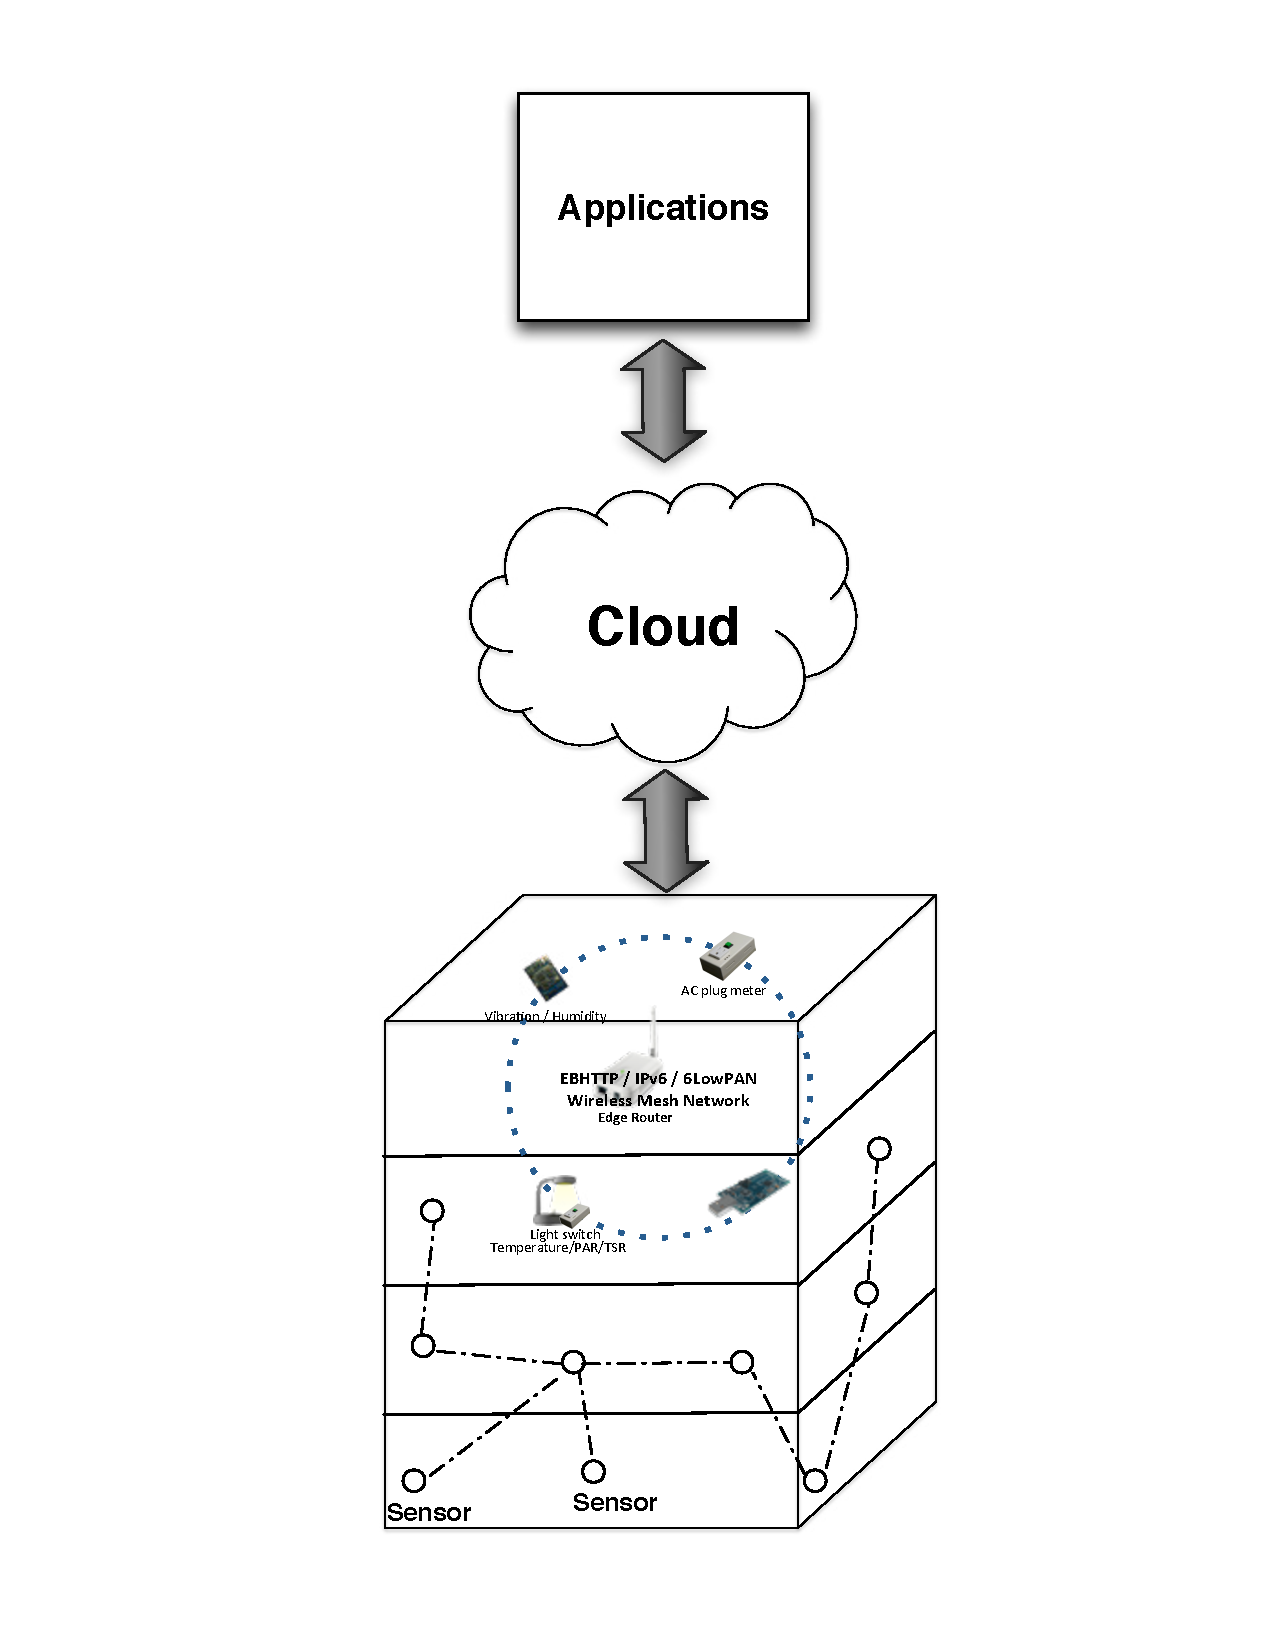
\includegraphics[width=0.5\textwidth]{figs/BuildingAppModel}
\caption{Building application model.  Building sensor deployments send data to the cloud and applications access it as it streams in.
Applications may also feed data to the cloud and make it available to other applications.}
\label{fig:buidlingapp}
\end{center}
\end{figure}



\section{Pervasive Computing}
The polifertation of cheap, networked, embedded sensors is moving us towards a future where our infrastructure is 
populated with computing that enable smart environments.  We march towards Mark Weiser's vision of the future of
computing \cite{uqicomp_vision} where the environment contains sensors, people interact directly with the 
physical objects in the environment,
and are better able to optimize performance of our infrastructure, uncover problems with wear and tear,
and share information with others that provide greater insight into the world around us.  This vision has be borne out
incremenetally in the research community since the vision was initially proposed over 20 years ago.

The research in this area starts from the vision for the field.  What could the world be if we are surrounded by computing?
How will we interact in that world?  What can we learn from the world and from each other?  Hypothetical scenarios
guide the early work.  A common scenario is one that makes use of a personal handheld device, ``smart'' objects, and 
ubiquitous connectivity.  Much of the early work was aimed at constructing a scenario that captures some aspect of
the future evisioned that can be used to highlight and explore fundamental challenges in realizing the vision.
For example, Christensen et al.~\cite{Christensen_2002} explore how pervasive computing will play a role in assisting
office workers in their day to day activities.  They imagine a scenario where members of an office each have mobile devices
and interact and share information with each other through serendipitous work-related interactions.  Through this scenario
they bring-forth fundamental issues related to mobility, interrupted operations, and activity scheduling due to ad-hoc 
collaboration.

Many fundamental challenges were discovered and addressed in this fashion.  Pervasive computing work eventually branched
off into several sub-domains with their own focus.  Some examples are work related to 
localization~\cite{Castro01aprobabilistic,Koo,Romer03thelighthouse,Yoon2013}, 
mobility and mobile devices~\cite{Haritaoglu:2001:ILR:647987.741331,Want02thepersonal,Jiang:2011:MPM:2030112.2030150},
context deduction and wearable computing~\cite{Holmquist01smart,Lukowicz2002,Christensen_2002,Rossi:2011:RWC:2030112.2030238},
and sensor networks~\cite{Conner:2001:MEL:647987.741329,Lymberopoulos09amethodology}.  These and related
topic areas have guided our thinking in addressing the problems in the building environment.

Looking back at the pervasive computing work, we observe that much of the work has focused on user but not as much on 
the challenges in the environment itself.  There is very little
emphasis on the infrastructure and issues with the accuracy in contextual representation of the physical environment.
There is also very little work on how a changing physical environment affects the accuracy with which applications can 
deduce the state of the world around them.  Also, there is very little emphasis on control of the physical environment.
The kinds of software processes that runs in buildings are primarily for control of the environment.  These issues
are neither addressed in the building science community nor the pervasive and computer science community.  We look at these
issues specifically in this thesis.


% Through the construction of vision-style scenarios and application development in those settings, 
% frameworks emerged and fundamental challenges were uncovered. 
% The challenges and solutions are related to localization, contextual inference, multi-modal input, vision, and other issues.
% Eventually each of these branched off into invidual fields of study and communities that examined these
% more deeply.
% As these communities matured they were driven by more realistic deployment and application contexts.
% Over the years, this evolution has included advantaces in sensing, mobile, and network technology but also computational 
% ubiquity through cloud computing.  Moreover, as we consider problems that emerge in specific application domains or
% industries, we will see that the convergence of these technologies allow new domain-specific problems and solutions 
% to be explored.


% Much of the work in computing in the built environment comes from pervasive computing.  Over the last
% 20 years, researchers have explored how computation can be used to capture the physical environment and
% how applications can be used to combine computational resources into a coherent service for users.
% Localization is a fundamental issue addressed~\cite{Castro01aprobabilistic,Koo,Romer03thelighthouse,Yoon2013}.


% % \begin{itemize}
% % % There has been much emphasis on wearable~\cite{} and mobile computing~\cite{}
% % \item Applications for connected devices
% % \item Infrastructure and tools (the environment advertises services, devices compose them and present them)
% % \end{itemize}
% Smart Objects, Context Awareness, Wearable~\cite{Holmquist01smart,Lukowicz2002,Christensen_2002,Rossi:2011:RWC:2030112.2030238}

% Sensor networks~\cite{Conner:2001:MEL:647987.741329,Lymberopoulos09amethodology}.

% Mobile devices and mobility~\cite{Haritaoglu:2001:ILR:647987.741331,Want02thepersonal,Jiang:2011:MPM:2030112.2030150}.

% Much of the work has focused on user but not as much on the challenges in the environment itself.  There is very little
% emphasis on the infrastructure and issues with the accuracy in contextual representation of the physical environment.
% There is also very little work on how a changing physical environment affects the accuracy with which applications can 
% deduce the state of the world around them.  Also, there is very little emphasis on control of the physical environment.
% One of the primary kinds of software processes that runs in buildings are for control of the environment.  These issues
% are neither addressed in the building science community nor the pervasive and computer science community.  We look at these
% issues specifically in this thesis.


% What's lacking?
% > Little to no emphasis on the infrastructure that is already there for collecting informationa about the environment.
% > All the work is human-centric with general components.
% > No emphasis on issues with the data itself and how we can infer context while the context is changing in the physical infrastructure itself.
% 	> No talk about controlling the environment.  Mainly a focus on provided context-deducing/aware middleware and applications.


\section{Cloud Computing, Ubiquitous Connectivity, and Mobile Phones}
Cloud computing has truly changed the way we design systems that bring together the physical and computational world.  Coupled with the 
continued maturation of networking technologies -- both indoor through Wifi and outdoors through cellular -- and the explosion of mobile
phone use, today's systems are designed with the mobile phone as an access tool for information in the cloud.  It is mostly safe
to assume that this information will be accessible.  Moreover, connection speeds can reach up to 300 Mbps, so serving sophisticated
applications from the cloud and designing them in a highly interactive manner is commonplace.  The main bottleneck is the form of interaction, which
is still a challenge given the small screen of a mobile phone.

This design pattern also makes it easier to combine everything into a single system that is centrally accessible.  So services in the cloud
can serve many clients simultaneously, proving a unified view of the state of the service and the object in it.  There is no difference 
between the desktop application and the mobile application, other than the way the service is presented to each.  Moreover, all the data
should live \emph{in} the cloud and be fetched \emph{from} the cloud by all clients.  The cloud service mediates interaction between all
participants in the system.

\section{Applications in Buildings}
Advancements made in the pervasive computing communities, trends in technology, and problems in buildings lead us to thrust of this thesis.
We start with the notion of ``app-ification'' of the building.  Technology trends have enable mobile phone ``apps''; mobile
applications that closely interact with content in the cloud.  We assert that a good way to address problem in the building
by opening up the building's sensor data streams and buildings services that make use of that data.  A system should provide 
\emph{uniform access} to the data and \emph{facilities for cleaning and aggregation}.  It should be \emph{extendable}
so that disparite systems could share information that could enable new kinds of applications.  Figure~\ref{fig:buidlingapp}
illustrates a high-level of building ``app-ification architecture''.

The building-scientist and architecture community already has a family of products and software pacakges that take building data an analyze
it.  We need to be able to support those as well.  The main idea is to open up the building and a system where innovation can take place.
We believe that the cloud-based service model would be effective.  Such service would contain a number of data services 
that enable data processing tasks to deduce the performance of the building.  The service should also enable control of the building
and help support holistic control applications that combine disparate data sources through the service itself.
We describe the design of such a system in Chapter~\ref{chap:SensingInBuiltMain}.


\section{Research Statement And Hypothesis}
We formally state our guiding research thesis and hypothesis:
% \emph{What are the architectural components and technical challenges in the design of an information system
% that enables new and supports old classes of applications in the built environment?}  
\emph{How can we incorporate filesystem and database constructs and what are the technical challenges in a system that supports applications
in the built environment?}
Given the emerging applications in
the built environment it is clear that the old information system design is not sufficiently open, flexibile, nor
scalable enough to support them.  Old information systems are tightly integrated from the field-level sensor to
the central supervisor control system.  There are two integration points in traditional systems that we argue 
are either fundamentally flawed or insufficient for emerging applications.  We describe the components that 
currently exist and identify those that are missing.  We show how these components/services enable emerging applications.  We also
discuss the technical challenges that must be solved in order to provide the correct semantics for these services.
Furthermore, we discuss a component that is fundamental for providing correct information to applications 
and formalize the notion of verification in the context of the built environment.  We provide several algorithmic 
solutions to these problems, which lay the foundation for a fundamental service in the broader architecture.

\section{Thesis Roadmap}
In the next chapter, we discuss building information systems today.  We dive into their architectural components and introduce some terminology
used in the building space.  We also describe the motivating scenario that they were built for and examine how well the architecture 
can support the ``app-ification'' of buildings.  We give examples of specific applications that we would like to support
and walk through the components that are useful for this purpose and those that are missing.  We propose a set of necessary
components in an architectural re-design that could provide the same support as BMS's today as well as the emerging ones that we
describe and argue that this should be the design of a \emph{building appification system}.

In chapter~\ref{chap:SFSArchMain}, we give an overview of a system we designed with the components we propose in the previous
chapter.  The name of the system is StreamFS. StreamFS is a cloud-based service that combines filesystem and database constructs
to organize the streaming sensor data, clean and process the stream, and provide a unified access layer to both physical information
and actuation channels in the physical world.  We discuss the overall structure of the components of the architecture and how
they interact with one another.

Chapter~\ref{chap:ProcMngtSchedMain} focuses on the process management component in StreamFS.  The process management component
manages the streams and the processes that consume those streams.  It is designed to support processes that are specified by the user
and managed by StreamFS as well as integrating external processing components and representing them through the file system in StreamFS.
We discuss some of the challenges and present some solutions to a scheduling problem related to providing fresh data  to processing jobs.
We also describe how various kinds of aggregation can be performed on the data, using the filesystem and pipe abstraction
presented and managed by this component.


Chapter~\ref{chap:naming} discusses how we represent the world as a collection of files.  StreamFS follows the unix filesystem principal 
where everything is a file and this allows us to provide a unified management layer for the entire set of building deployment
data and metadata.  We discuss the individual file types that we support and their semantics.  We also introduce the fundamental
challenge of dealing with evolving metadata.  Specifically,  we show how changes in the physical world can present problems
with the structure and relationships between the files in the system.  We show the basic set of tools that we use to address these problem
at the end of the chapter.

We evaluate the StreamFS in chapter~\ref{chap:ArchEvalMain}.  We describe our experience in deploying StreamFS in several buildings
at UC Berkeley and the University of Tokyo.  We describe these deployments in the context of 4 applications: 1) a deployment viewer
application, 2) a real filesystem mount and direct integration with a legacy applications, 3) a real-time visualization and 
aggregator tool, and 4) a combination of the other applications with a mobile phone fo energy auditing.  We also give an overview of the
application programming interface and discuss how StreamFS can help build generable, scalable re-useable software within
buildings.

Finally, we discuss verification of building systems and metadata in chapter~\ref{chap:VerificationMain}.  We introduce 4 types of 
verification and describe why each of them is crucial to building applications that interact with the physical world through
a layer of software represent it.  We discuss our work on the Strip, Bind and Search methodology for functional verification, 
our use of mode decomposition for spatial verification, and timeseries clustering techniques for type classificaiton.  We
describe value verification but do not present any results in that area.
We discuss future work in chapter~\ref{chap:future} and conclude in chapter~\ref{chap:done}.





























\chapter{Sensing in the Built Environment}

Buildings consume nearly 40\% of the total energy produced in the United States and 72\% of the electricity.  Similar figures 
have been recorded in other industrialized countries~\cite{buildings_study}.  Furthermore, studies show that they waste from
30-80\% of the energy they consume.  With specter of global warming and the continued decrease in the cost of storage and 
communication, buildings have become a major target for improved energy efficiency.

Large commercial buildings typically contain thousands of sensors embedded in them which report periodic readings to 
a centralized system called a building management system.  Typically these have been installed for supervisory control and
centralized observation of the building.  The kinds of sensors installed including temperature sensors on the thermostats,
valve position meters and actuators on pipes, pressure sensors in the vents, temperature sensors on the vents and pipes, etc.
These readings are combined with a graphical interface for building managers to visually locate them according to their location.
The interface also allows them to visually inspect and quickly try to diagnose a problem, typically in response to occupant
complaints.

Although these systems have been revolutionary from a building management perspective, they lack many fundamental components for
truly enabling sophisticated analysis -- the kind of analysis that is needed to understand how the building is performing
and will perform in the future.  Also, building practices for software-driven building systems serve more as guideline than
 as a standard.  This presents major challenges with respect to software re-use and scalability.  In this thesis
we will discuss the how we address these challenges through architectural design choices and analytical metholodology.  
The achitectural choices reconstruct the software layer that sits on top of existing building management systems and presents
a unified interface and standard API for analytical and control building applications.
The analytical methodology offers a general approach to verifying the construction of point names -- the naming scheme for 
sensors distributed throughout the building.  Both set a foundation for ongoing and future work.

The thesis is presented in the context of building systems and building-related applications.  We draw out the fundamental 
components in our analysis and design and discuss where it fits in the broader context of prior, computer science related,
literature.  In the next section, we describe the state-of-the-art practices followed by vendors of building information systems.
We describe the architecture features and design principals both implicitly and explicitly implemented into these systems.
We present the pros and cons of these decisions and their implications and include a high-level description of our approach.
Later chapters delve more deeply into the implications of our design decisions.

\section{Tightly Integrated Building Information System Architecture}

The first building information systems became commercially available in the 1970's ~\cite{gardner1987energy}.  
Historically, building management 
systems were constructed as a collection of control loops, which progressed from pneumatic to analog to digital.
These control loops largely form the foundation for the design decisions made in building information systems.  
This section gives a quick overview of the architecture, bottom-up and describes how each stage is built around
the concept of loops and supervisory control.  We then describe some of the short-comings of this architecture
and give an overview of how we address it in a system called StreamFS -- described in more details in
the remaining chapters.

\begin{figure}[t!] %htbp
\centering
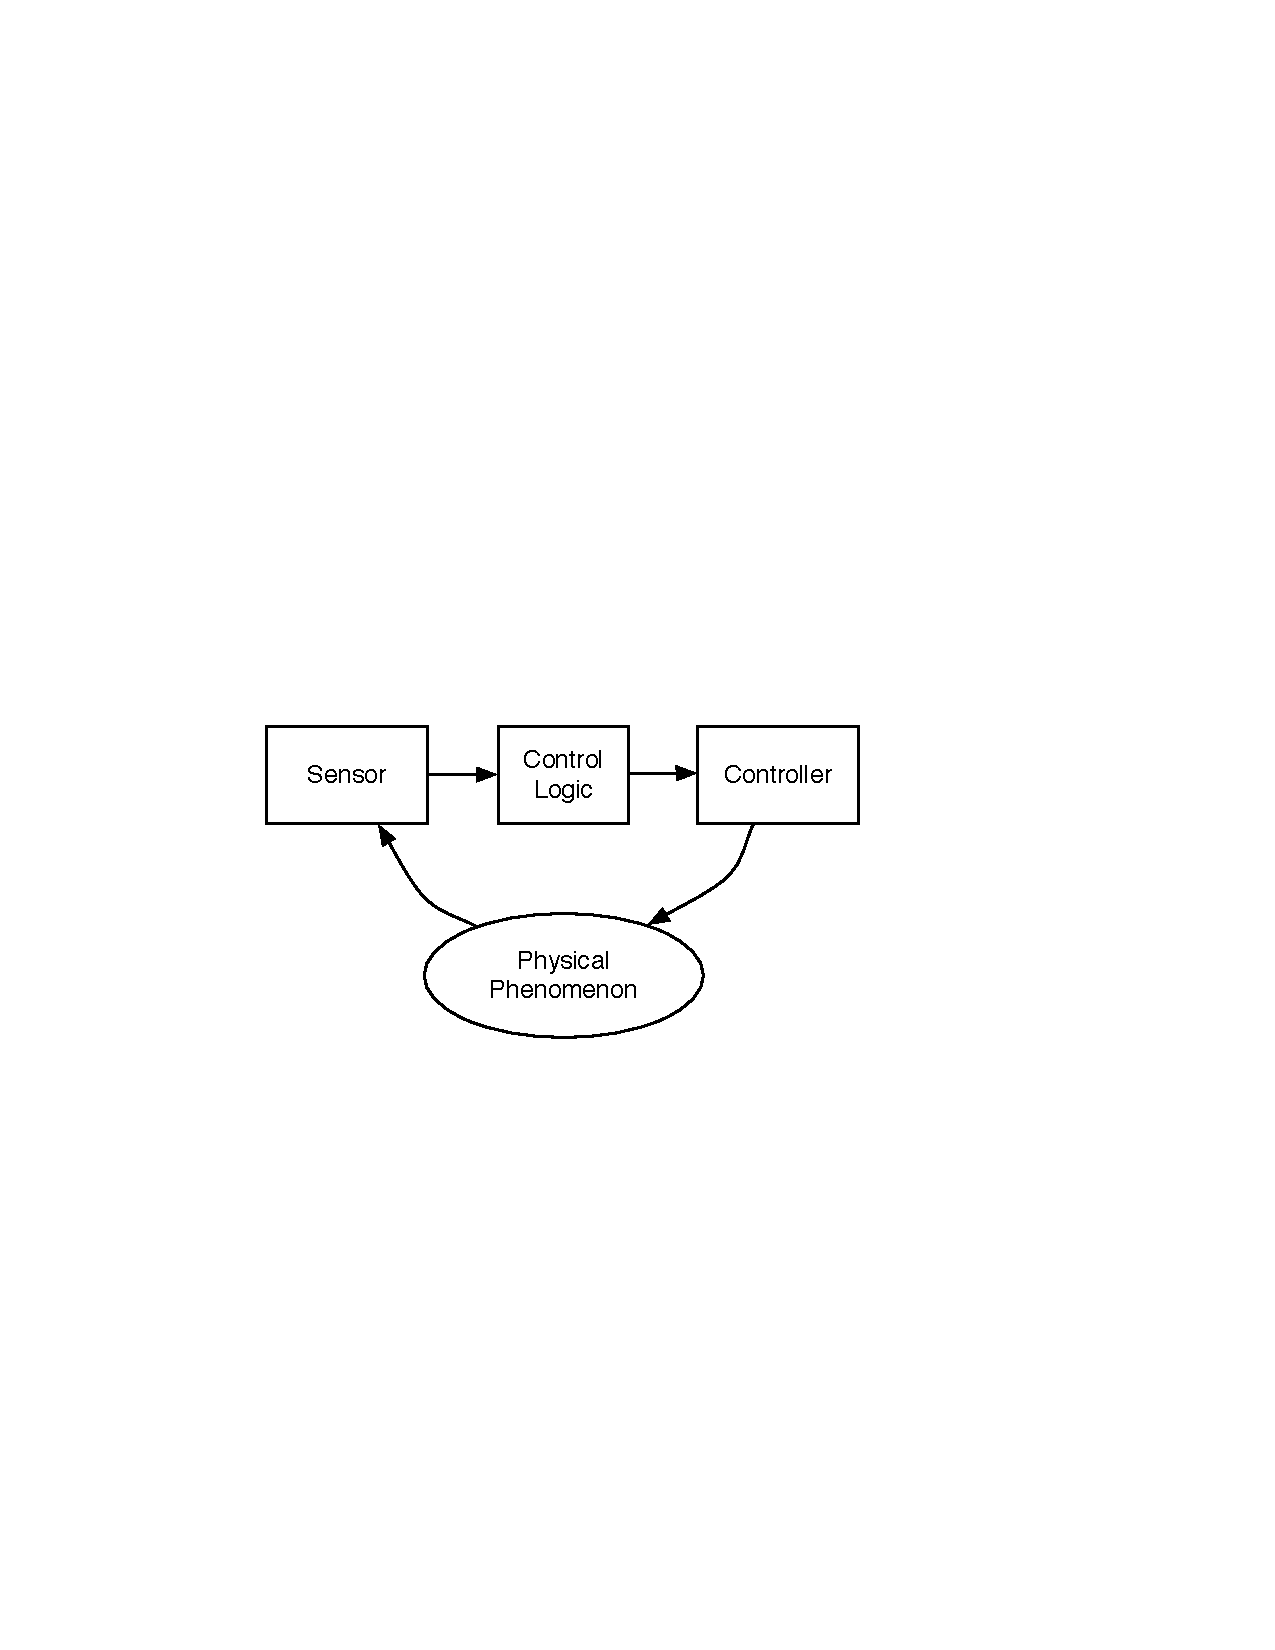
\includegraphics[width=0.50\columnwidth]{figs/control_loop}
\caption{General building control loop.}
\label{fig:control_loop}
\end{figure}

\subsection{Control Loops and The Outstation}
\label{sec:control_loops}
Each loop is defined by a control domain consisting of a sensor, an actuator, and a control mechanism.  The control mechanism
become logic based when signals from sensors moved to the digital domain.  However, the basic control principle is based
entirely on local control loops, with the implicit assumption that these loops are independent.
Figure~\ref{fig:control_loop} shows a high-level control loop.  A simple control loop in the building is one that controls
the temperature in a space.  It has a temperature sensor as the input and uses the temperature set-point parameter to 
decide when and which actuators to activate.
For temperature control, this actuation controls the the vent that lets cool air into the space.  This causes the temperature
to fall until a lower-bound is reached and the control logic re-activates the fans and heating/cooling system.

The figure also shows the basic structure inside an outstation.  An outstation is a box that contains up to several control boards, each
wired to one or more sensors and one or more actuators.  The outstation is typically close to the sensors and actuators (in the same room)
and contains all the control logic for the local plant.  Inside the control logic there is a CPU and some memory.  The memory
contains the control program and some space for sensor readings.  It is directly wired to the sensors and actuators through
a series of buses and shown in Figure~\ref{fig:control_box}.

\begin{figure}[t!] %htbp
\centering
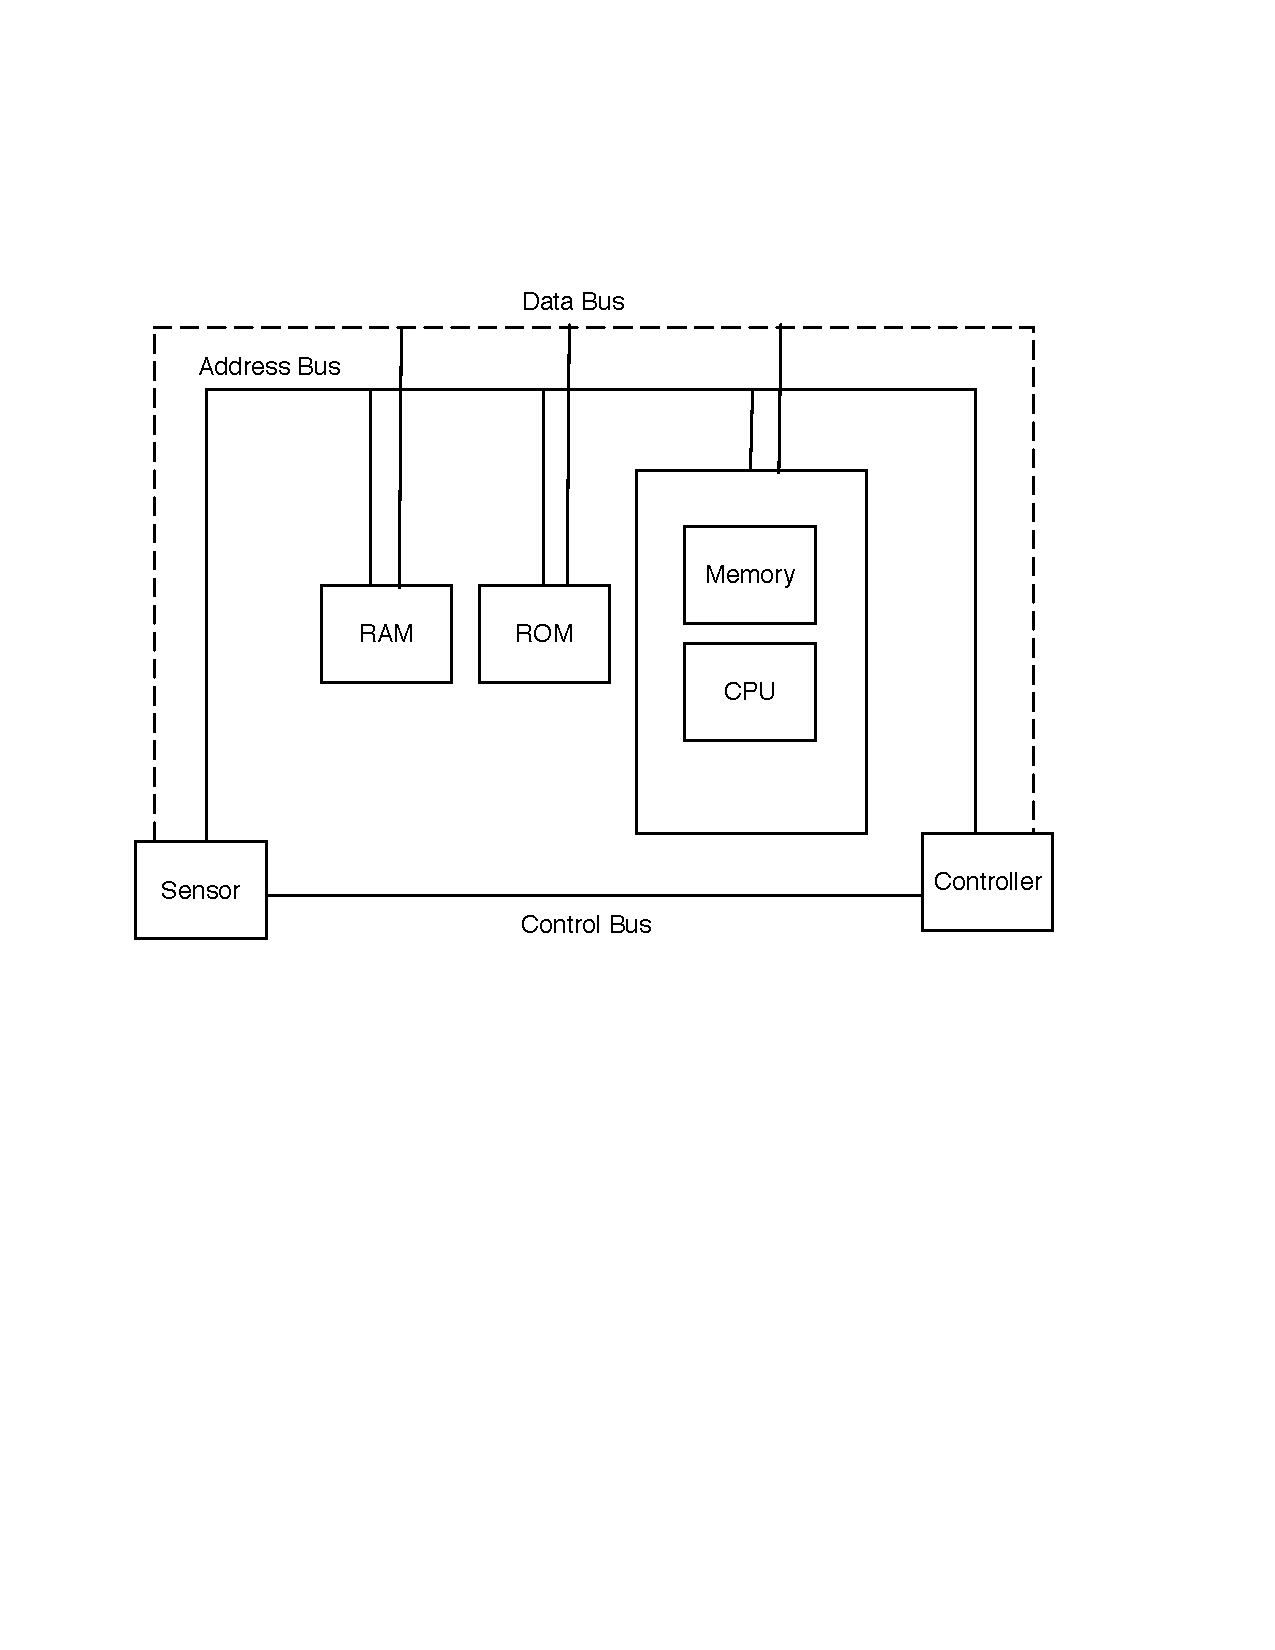
\includegraphics[width=0.50\columnwidth]{figs/control_box}
\caption{High-level control board architecture.}
\label{fig:control_box}
\end{figure}

As readings from the sensors are taken, they are placed in RAM.  The amount of RAM is limited and can get filled up, so it is important
to schedule periodic collection tasks from the central station -- the building management system (BMS).  The control logic is typically
written in ROM and can only be changed by the equipment or BMS vendor.  The input parameters are set at the BMS and they dictate the operational dynamics
of the control scheme in reaction to the input~\cite{BMS_book}.
Outstations are distributed through the building and are essentially running independent of one another.  In order to enable centralized 
monitoring and control, they are networked together and report some of the sensor readings and control-logic state to a central outstation.

\subsection{Central Outstation and Communication Protocols}
The central outstation is typically a Microsoft Windows-based PC connected to the outstation through either RS-485/modbus or Ethernet.
The user interacts with the system through a graphical interface, constructed from the schematics for the building or the schematics
for the component in the system that is being monitored.  The BMS running on the PC communicates with outstations through either a 
vendor-specific, proprietary protocol or an open one like BACNet~\cite{Bacnet} or LonTalk~\cite{LonTalk}.  Note, 
we focus on BACNet, but the similar features exist in other protocols, such as LonTalk.  

\begin{figure}[h!] %htbp
\centering
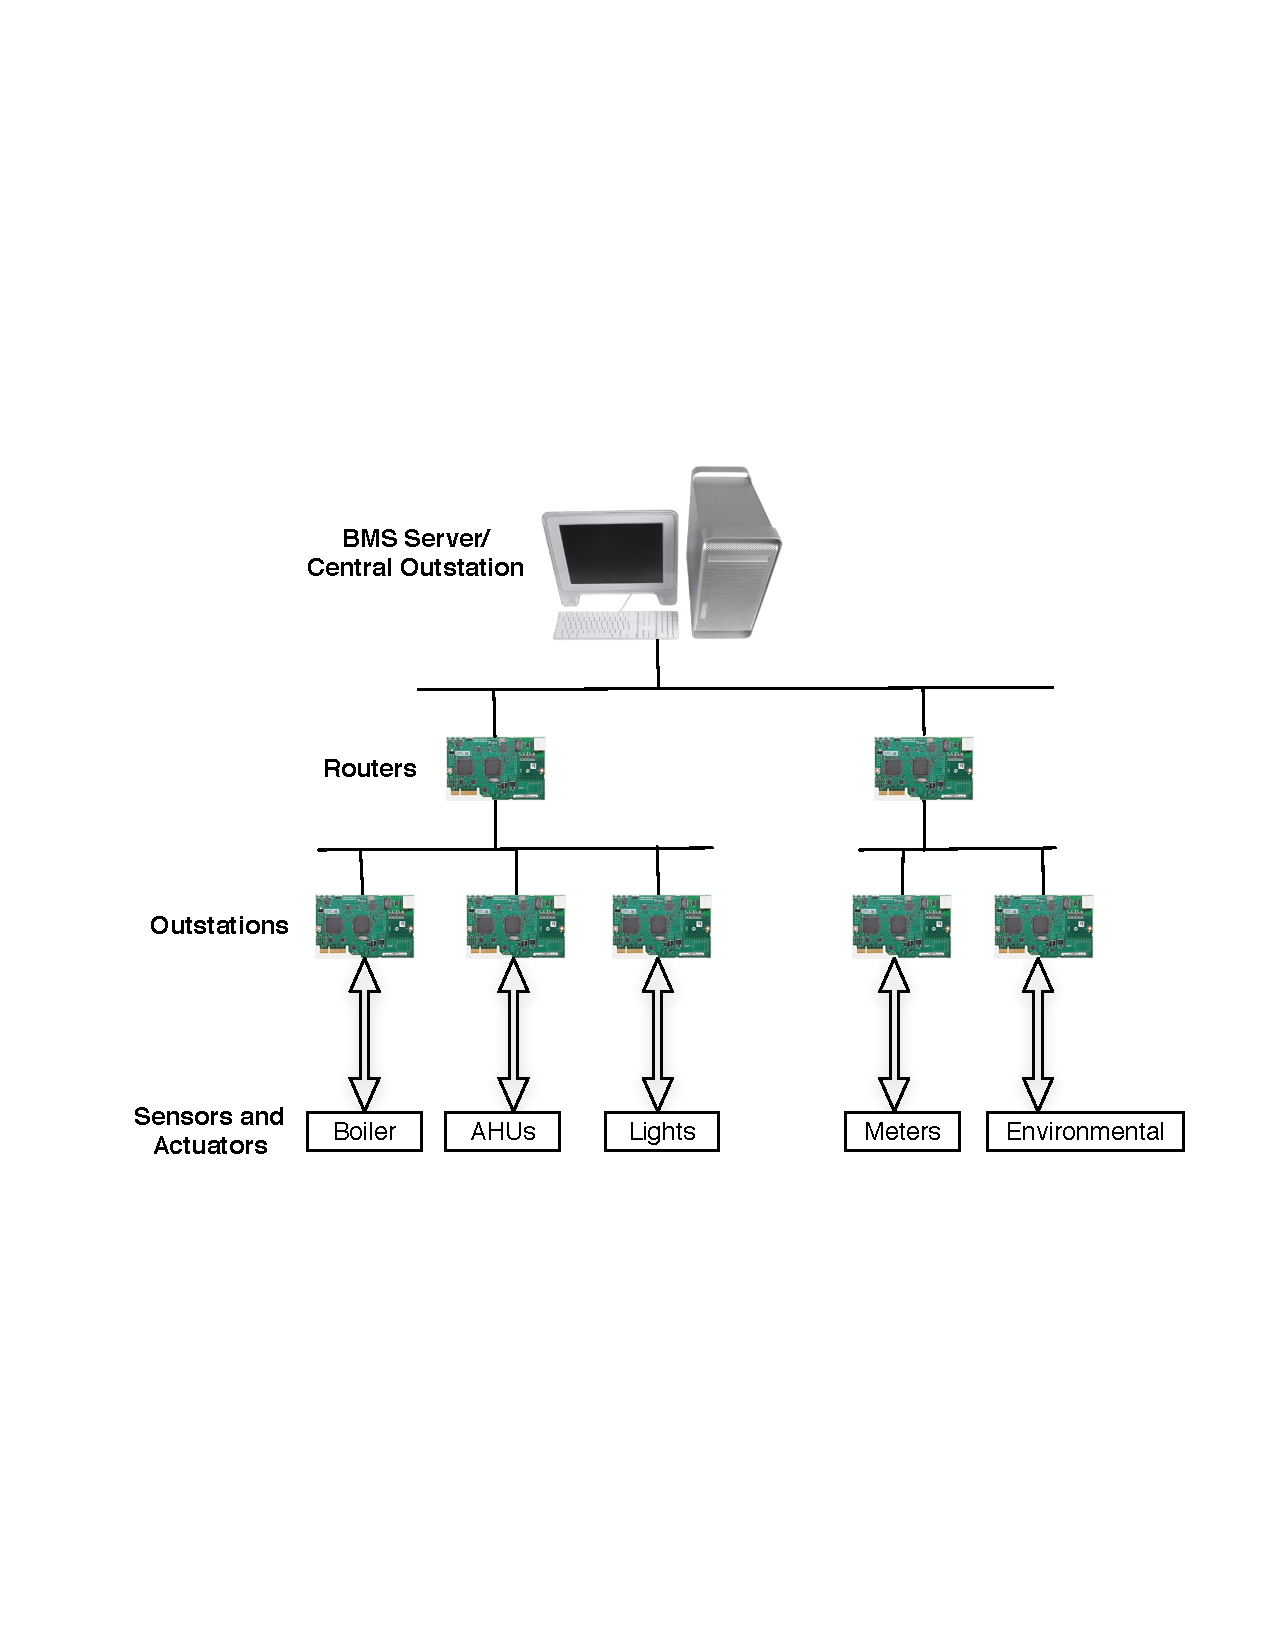
\includegraphics[width=0.50\columnwidth]{figs/BMS_network}
\caption{BMS network architecture.}
\label{fig:bms_network}
\end{figure}

Both protocols define both a wire protocol and packet structure for communicating with outstations and each other.  They also define a high-level
naming scheme for sensors in the building, called `points'.  A point can also refer to a non-physical object, like a schedule of operation.
It is common for both lights and temperature sensors to run on a daily, weekly, and seasonal schedules.  Such schedule are captured
by the \emph{schedule object} in BACNet.  
% BACNet also exposes devices as a collection of different object types.  
Each object contains a set of properties that can 
be read and/or written.  A device is identifiable through a name or address on the network, each object has a unique identifier and is one of
many types.  Examples of object types includes the following: input, output, value, analog~\cite{Bacnet}.  

These protocols also provide a mechanism for discovery .  Each [device, object name/id, property name/id] tuple forms a name.
This name is exposed by the protocol-server to the application.  All the names are set by the vendor and the are shown through the graphical interface
of the BMS.  
% constructed from the building schematics, is also designed and constructed by the vendor.  
The building manger is the primary user of the BMS,
so rather than expose the underlying protocol, he/she interacts with the building via the graphical interface.

In order to interact with the underlying sensor and actuator layer, the application must use a stub that communicates directly with the 
sensor/actuator through the BACnet stack.  External communication stubs are recognized similarly to sensors/actuators.  They are represented 
as a collection of 
objects with readable/writable properties.  An example service that is provided in BACNet is  \texttt{WhoIs} and \texttt{EventNotification}.
The former is a broadcast service that is used for discovery of other objects, the latter is used for setting alarms on the sensor data that
are reported by the BACNet enabled devices on the network in the outstation layer.  There are many other types of events that are supported 
and over 50 types of object types in the baseline protocol, which is extensible.  Device and object names that are added have no restriction
on either the number of characters (specified by the vendor) or the encoding.


\begin{figure}[t!] %htbp
\centering
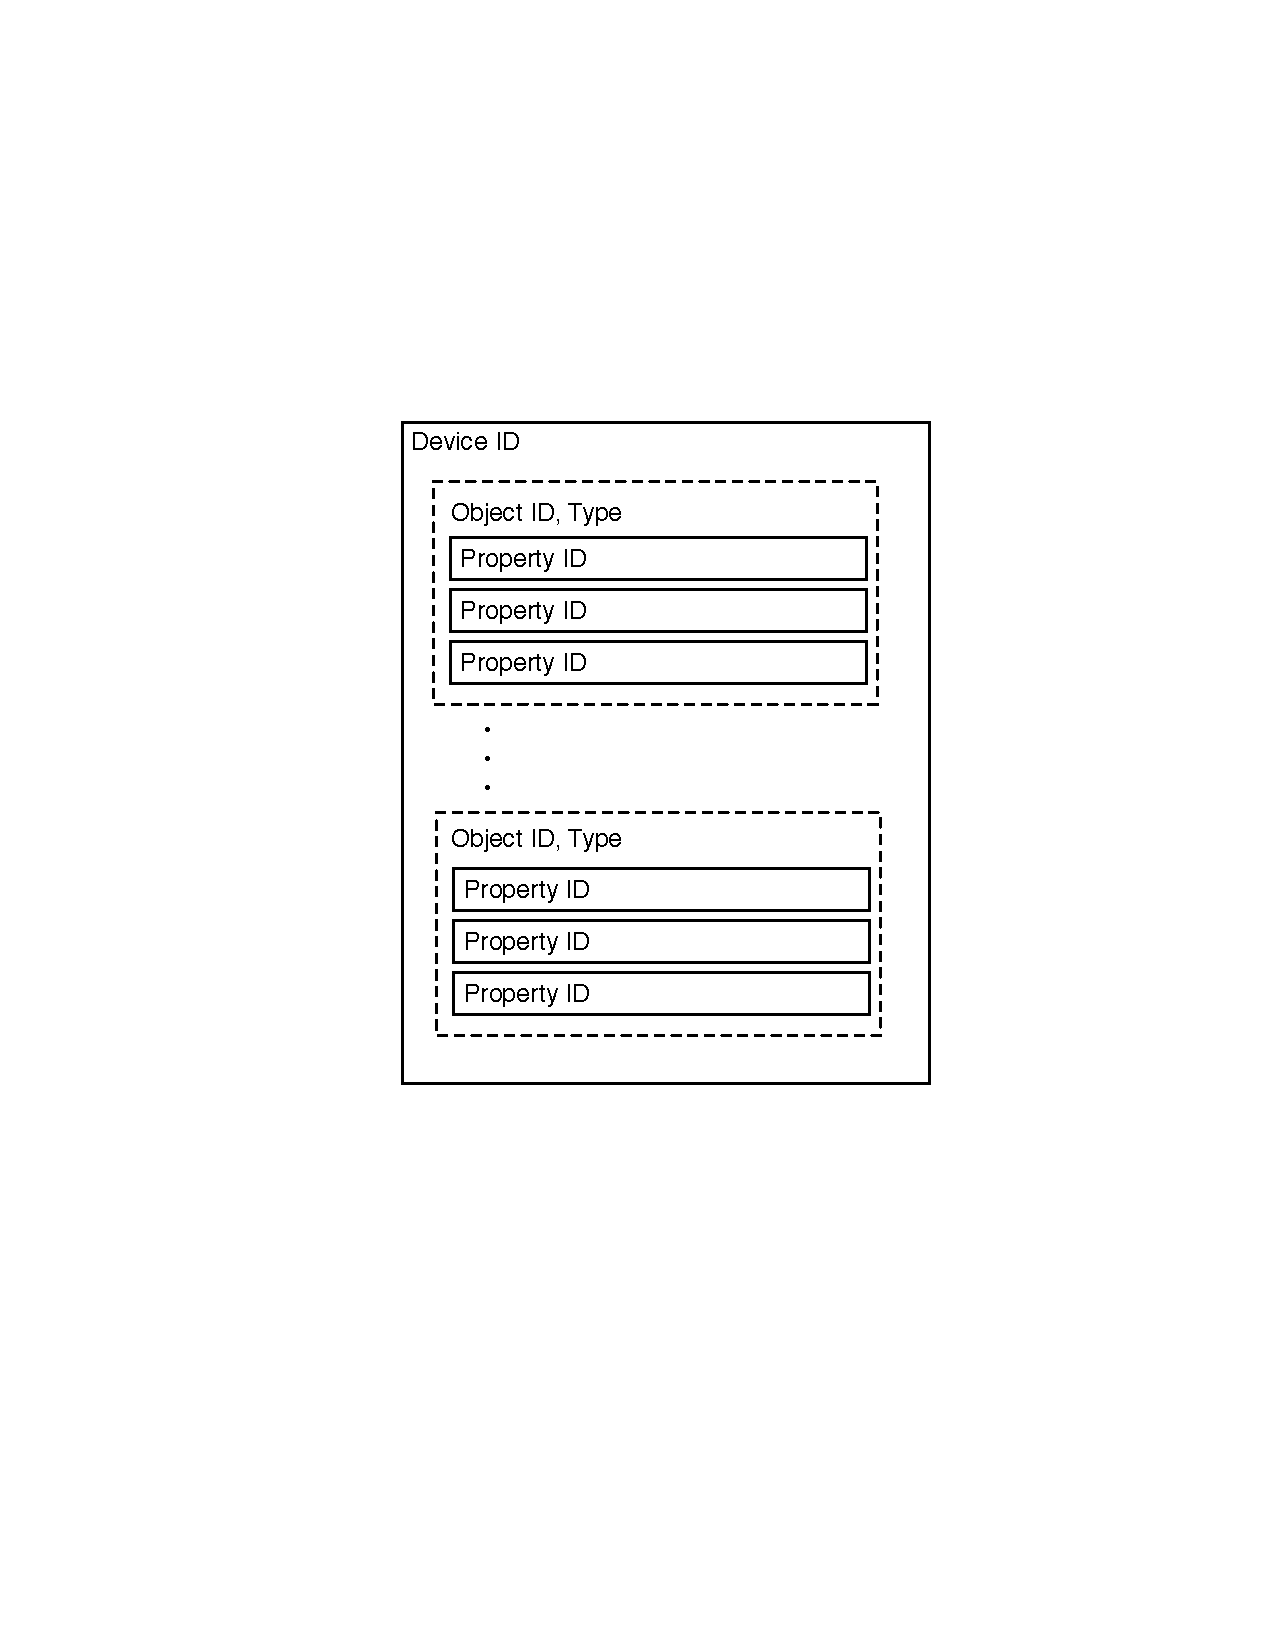
\includegraphics[width=0.25\columnwidth]{figs/bacnet_device}
\caption{BACNet device example.}
\label{fig:bacnet_device}
\end{figure}
\section{From Supervisory Control to Application Development in Buildings}
%From Supervisory Control to Application Development in Buildings

% Building information systems were built as tightly integrated silos, where the main application is the graphical user interface.
Features for interoperability were designed at two interface layers: 1) the protocol layer and 2) the presentation layer through a
data-export feature.  The protocol layer provides services for enabling devices to talk to one another through the network.  
Several features were explicitly designed around
the notion of interoperability: trending, scheduling, management services, alarms and events, direct sharing.  The graphical
interface layer is mainly focused on providing periodic reports in a comma-separated value (CSV) file, which
contains point-name information and time-value pairs of data.
% Historically, the extent of interoperability objectives has included mainly the introduction of new devices onto the network or
% the exporting of data for other software program to use for analysis and report generation.  
For these protocols, interoperability means adding new devices or exporting the data in a common format.
Building information systems themselves
were built to mainly support the in-time management and supervisory control of the building.  Analysis does not 
extend far beyond univariate plotting and individual assessment of equipment and control.  Most tuning of control parameters is 
manual.  Hard-wired control logic at the outstation is rarely updated.


Over the last few years, however, there has been in increased interest in energy management and comfort as a primary objective 
in the design of new building applications~\cite{6146507,Yu1956572,Mamidi2343582}.  Moreover, there is a broad interest in buildings
using global control schemes to optimize their performance and to interact more efficiently in response to renewable sources and its  
generation volatility~\cite{Taneja2223873,5985456,Lu2009}.  Model predictive control has introduced new ways of controling the components in the building
to make them more energy efficient~\cite{mpc}, there is an interest in performing dynamic, real-time analysis of building health
and efficiency~\cite{dynamicLeed}.  There has even been interest is improving the visibility of the state of the building to the 
occupants through various modalities, including touch-screens and mobile phones~\cite{andrew_lighting, Hsu1878444, Ortiz2422540}.  
These, and other emerging applications,
have pushed the boundaries of demand beyond what a modern building information system can provide and a re-design must be considered.
\section{BMS Architectural Shortcomings for Supporting Emergying Application Development}

\begin{figure}[t!] %htbp
\centering
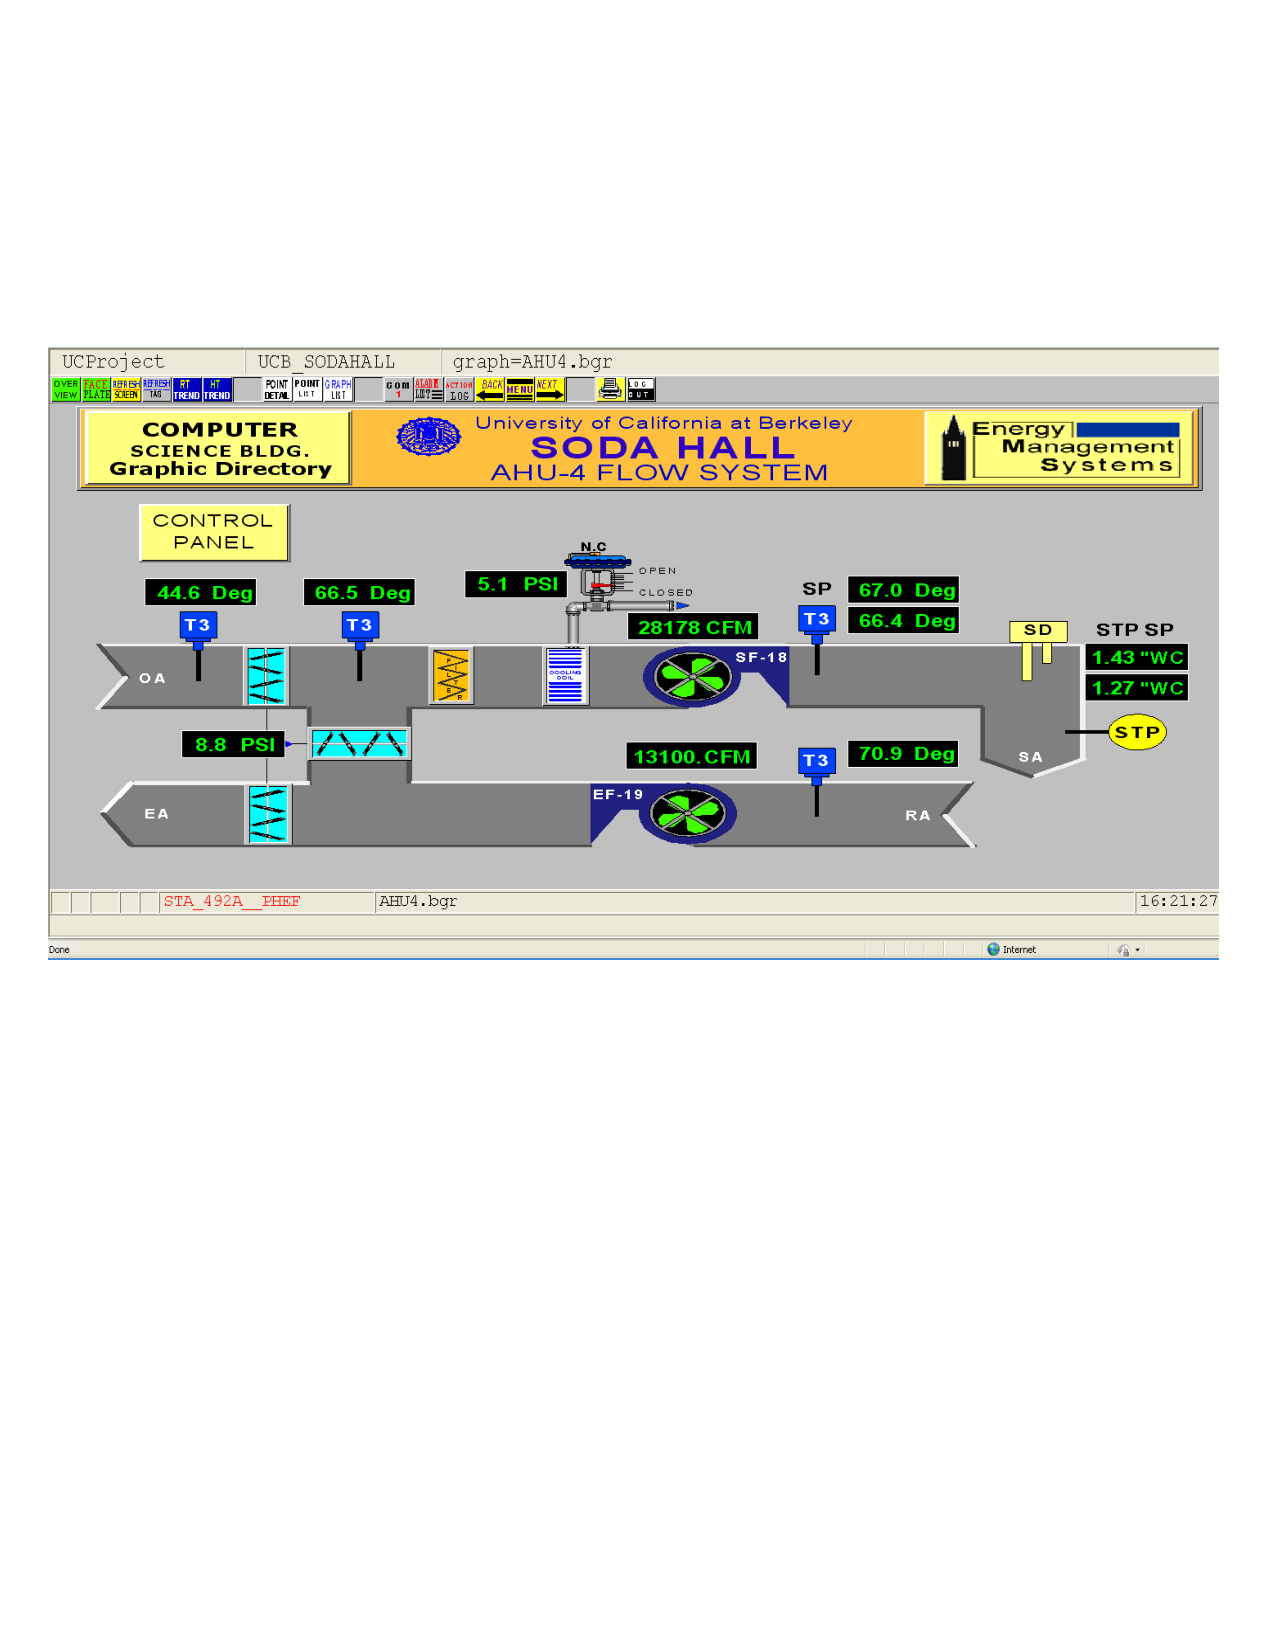
\includegraphics[width=0.75\columnwidth]{figs/soda_bms_screenshot}
\caption{Screen shot for the Soda Hall Building Management System Interface.}
\label{fig:soda_bms_screenshot}
\end{figure}

% In this section we dissect the current architecture in the context of current and future applications
% for buildings.  The first two describe how the current architecture is used to provide the intended service
% that these application provide.  The latter two are emerging applications that we would like to available
% throughout the entire building stock.  We will see, however, that these are very difficult to build at scale
% and we pose the question ``what is missing in the current architecture to enanble the system properties that help
% support these and other emerging applications?''.  Through close inspection it will hopefully become clear that
% the current architecture is fundamentally flawed; built largely to support a small set of vendor-specific
% applications and not much else.

% In this section we dissect the BMS architecture and closely examine how well it can support broad application development
% in buildings, rather than the single supervisory control function it supports today.  
We examine today's BMS architecture in the context
of 4 potential services with distinct operational requirements that need to be supported.  The first two services that 
are offered today and enabled by the BMS.  We describe how emerging requirements are driving the evolution of these
services and how BMS's are struggling to meet the new requirements due to limitations in their architectural design.
The next two are emerging services that BMS's cannot support today.  We describe which architectural components must be included
or how current components must be modified in order to support these.  We also make the broader argument that 
building systems should be built to support a much wider range of applications that we cannot currently anticipate.
We will show why this requires a fundamental re-design and propose an architectural composition for such a system.
In the rest of the thesis, we will examine an instance of our architecture and describe the challenges in realizing
the use and effectiveness of our system in real building deployments.

% while the latter are potential applications we imagine will be supported in future
% smart buildings.  Through this exercise, we build our argument for a systematic re-design of such systems and propose
% a set of necessary architectural components necessary to enable and support emerging applications.

\subsection{Monitoring and Supervisory Control}
The primary objective in the design of building information systems is for centralized monitoring and supervisory
control.  Control algorithms are left ``to the expert'' and embedded in the outstation control board.  The intended
user of the system is a building manager -- a user whose expertise is much broader than the designer of the control
algorithm that runs on a particular system component.
The manager is expected to monitor the health of building systems and quickly diagnose problems when they occur.  The tool
is mainly in place to save the building manager time; and it is very effective at doing so.  The extent to which 
the building manager is making control decisions is altering control algorithm paramter setting through
the building management interface itself.  Even these decisions typically go through the vendor, through consultation.

Figure~\ref{fig:soda_bms_screenshot} shows a screenshot of the BMS in Soda Hall at UC Berkeley.  This specific image
captures a schematic for one of the air handling units.  It shows the various sensors embedded in different locations
on the component -- on either side of the supply/exhaust fans, temperature sensors at the supply/return sides of the
air ducts and the inlet vent, measuring the outside air temperature.  Accompanying real-time readings are juxtaposed
by the sensor image.  The user can double-click on the sensor or reading to get more information about that particular 
measurement point.  For example, if you double-click on a temperature sensor, it will give you the exact name of the 
point and accompanying information about related points, such as the set-point, which effectively drives the behavior of 
the underlying system.  If an occupant makes a complaint about not getting any air from the vents, for example, the 
building manager can find the screen for the vents that serve the room the occupant is in and observe the current
pressure readings or look for value-based alerts on any of the readings, typically displayed on the same screen.
If there is a malfunctioning component or something stuck in the vent, the readings should ``look off'' to the building 
manager.

If the problem recurs often, the astute building manager may be able to characterize the fault through a series of alarms.
They can be proactive about finding and fixing the problem(s) before they occur.  Alarms can be set through interaction
with the graphical interface, in much the same way that a lookup on the measurement point occurs -- by double-clicking on 
the point in question and following instructions for setting an alarm.  In some cases, the problem may be driven 
by a faulty setting and adjustments can be made to the control parameters through the associated control points.

The scope of control is limited to specific control loops.  Recall our discussion of control loops in section~\ref{sec:control_loops}.
The building manager can, typically with the help of the vendor, decide on the best control strategy setting.  If the control
strategy cannot be met, due to flaws in the control algorithm itself, the vendor may step in and re-image the controller
at the outstation and expose the necessary parameters through the graphical interface.  These kinds of changes are rare
but do happen occassionally and can be somewhat expensive, since the cost is not typically included with the purchase
of the system.  Because of the cost, the decision is typically made after close inspection and analysis, which a BMS
enables through the data export feature.  
For example, the sense/control points in question may be placed in ``trend'' mode.  This means that readings
from those streams are stored in the local memory buffer at the outstation for some period of time.  If a report is specifically
set up at the central system, a report period is also associated with the point, allowing the saved points to be drained
from the local buffer at the outstation.  The points are then placed in a file for observation and graphing by the 
building manager.  Time-dependent inspection of the behavior of any of the control-loop related points can be examined.

Although this feature is not necessary in order to change control paramters, it is useful for observing how parameter changes
affect the behavior of the system.  The building manager can, in principal, experiment with different setting and allow
empirical observations to guide her future decisions.


\subsection{Energy Auditing and Building Modeling}
Recently there has been renewed interest in the energy consumption of buildings.  In particular, several studies~\cite{BuildingEnergyData,
MITBuildingScience} show that buildings consome a large fraction of the energy produced in the United States and that as much
as 80\% of it is wasted.  As such, there has been an emergence of several companies and services for assessning the health of
commercial buildings with respect to their energy consumption.  Organizations such as LEED~\cite{Leed} provide certification of 
buildings, specifically rating the energy efficiency of the building.

Building modeling has been part of building science for quite some time, with systems such as EnergyPlus~\cite{eplus}.
EnergyPlus and simulators like it are part of a larger ecosystem of software for modeling various aspect of the operation
of the building.  They allow the designer to construct detailed models of the building, from construction to usage.  You can
model everything from the material, location, zone-based usage (office building, bathroom, storage room), window size and its
construction, etc.  There are different types of LEED certification, but typical certification requires the submission of the detailed
model and the results of various energy-related metrics, aggregated over seasonal time intervals to attain LEED certification.

Detailed model construction can take several months and in order to ground the underlying model in empirical performance data
typically a modeler will use the data obtained from the building's BMS.  Most vendors provide a way to export the point-related 
trended data.  Complex models can be built using this information.  The file export feature in combination with the ability to 
``trend'' points provide an interface mechanism for these and other kinds of applications that need to make use of the data.

Another option is to obtain the data directly from the system through the network.  Third-party vendors provide systems that 
will join the building network of devices and eavesdrop of the readings and traffic being reported to the central server.
This is the only way to obtain truly real-time readings from the sensors on the network.
Typically BMS vendors do not like this since they may generate too much traffic and overwhelm the network because of congestion.
Although not fundamental, it is a common concern in buildings today.  Many buildings use RS-485 rather than ethernet and there is
a general, albeit unfounded, concern that the network will become overwhelmed if all the points are trended and report at the same
time.

Building modeling and real-time analysis have been separated because of these constraints.  The constraints are largely not
fundamental, but the current architecture is simply not designed to provide real-time readings for \emph{all the points, simultaneously}.
Also, it is clear, even from the fairly simple workloads generated by these analysis applications, that a history of readings
is needed.  BMS's, as currently designed, require the end-user to manage the history of the data point individually.
When BMS's were first designed, there were certainly concerns about bandwidth and storage limits.  However, today those concerns
are a non-issue.  A few hundred bytes produced on the order of a few minutes, even from several thousand sensors is simply not
that much data.


\subsection{Holistic Building Optimization}

\begin{figure}[t!] %htbp
\centering
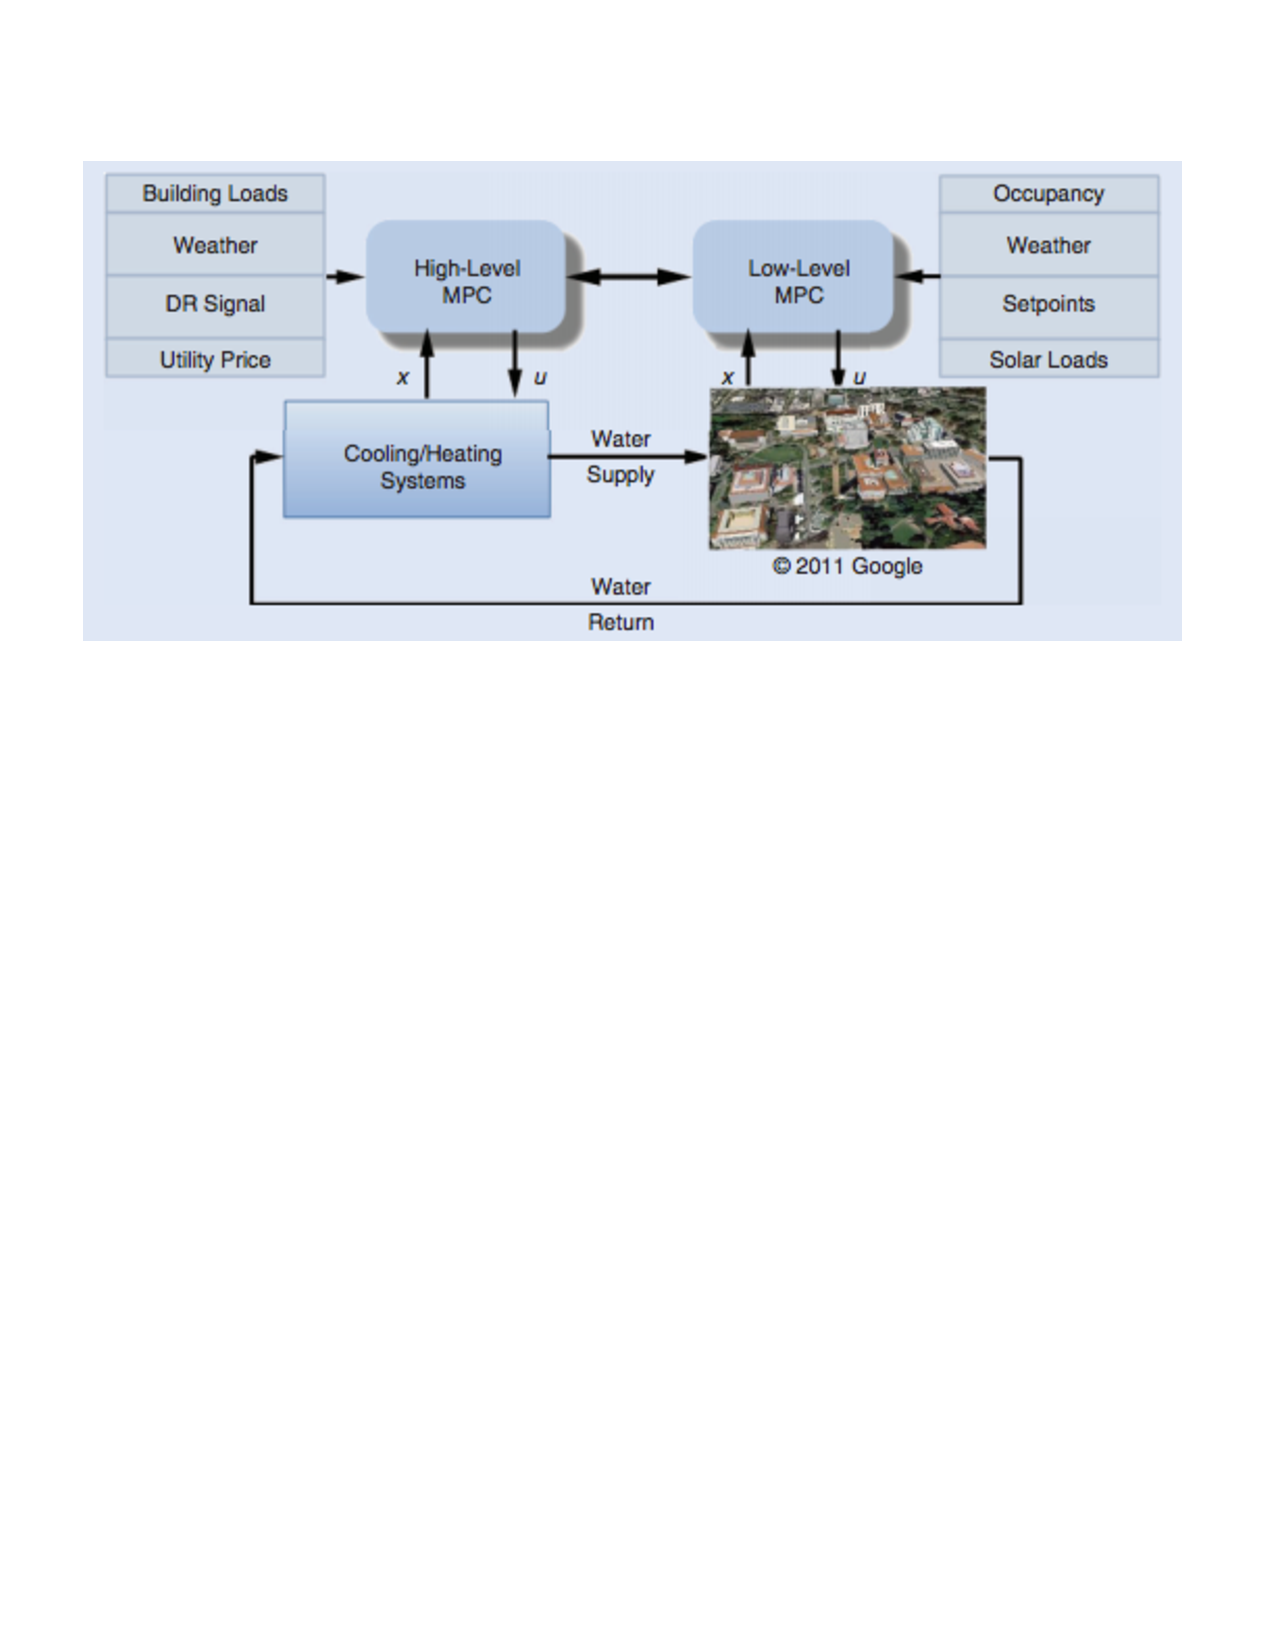
\includegraphics[width=0.75\columnwidth]{figs/mpc1}
\caption{Emerging Application: Hierachical MPC for a stock of buildings.}
\label{fig:mpc1}
\end{figure}

An emerging class of applications, is in holistic control of the building using a new technique called model-predictive control~\cite{MPC}.
Rather than rely on specific changes to control logic at the local-loop level, MPC techniques observe and learn a model
of the behavior of a components, multiple components, or the whole building, based on the historical data.  Once the model is learned, 
constraints can be specified to drive the behavior of the system to an optimal region in the tradeoff space; solving it as 
a constraint optimization problem.  Figure~\ref{fig:mpc1}, reproduced from~\cite{MPC}, shows an example of the how MPC combines 
several points in the building to control the building.  Essentially it decomposes a large optimization problem into indivial control 
decision to be made at the control-loop level.

In order to build this application, the set of necessary points must be mapped into the process.  The user, setting up the problem,
must connect the right data streams and control points to the algorithm by either manually going through the schematics or
locating the schematic representation in the BMS graphical interface.  There is no query interface and it requires that you sit
with the building manager or vendor in order to set up the trending, reporting, and enable the necessary control permisions.
The process is time consuming and \emph{does not scale}.

Although the method is very useful and has yielded excellent results, it is difficult to replicate.  The code and setup must be 
customized for each building or stock of buildings it is set up on.  This lack of generalizability and scalability is missing
in the current state of the art of building information systems.  In most cases the representation of sensor/actuator association is 
implicitly represented in a combination of the schematics, the graphical interface, and the point name.  Moreover, all
three of these change from building to building.  It is fundamentally difficult to generalize.  Buildings are treated as one-off constructions
and their associated digital information has historically followed the same principle.


\subsection{Personal Energy Viewer}
\label{sec:mobile}

\begin{figure}[h!] %htbp
\centering
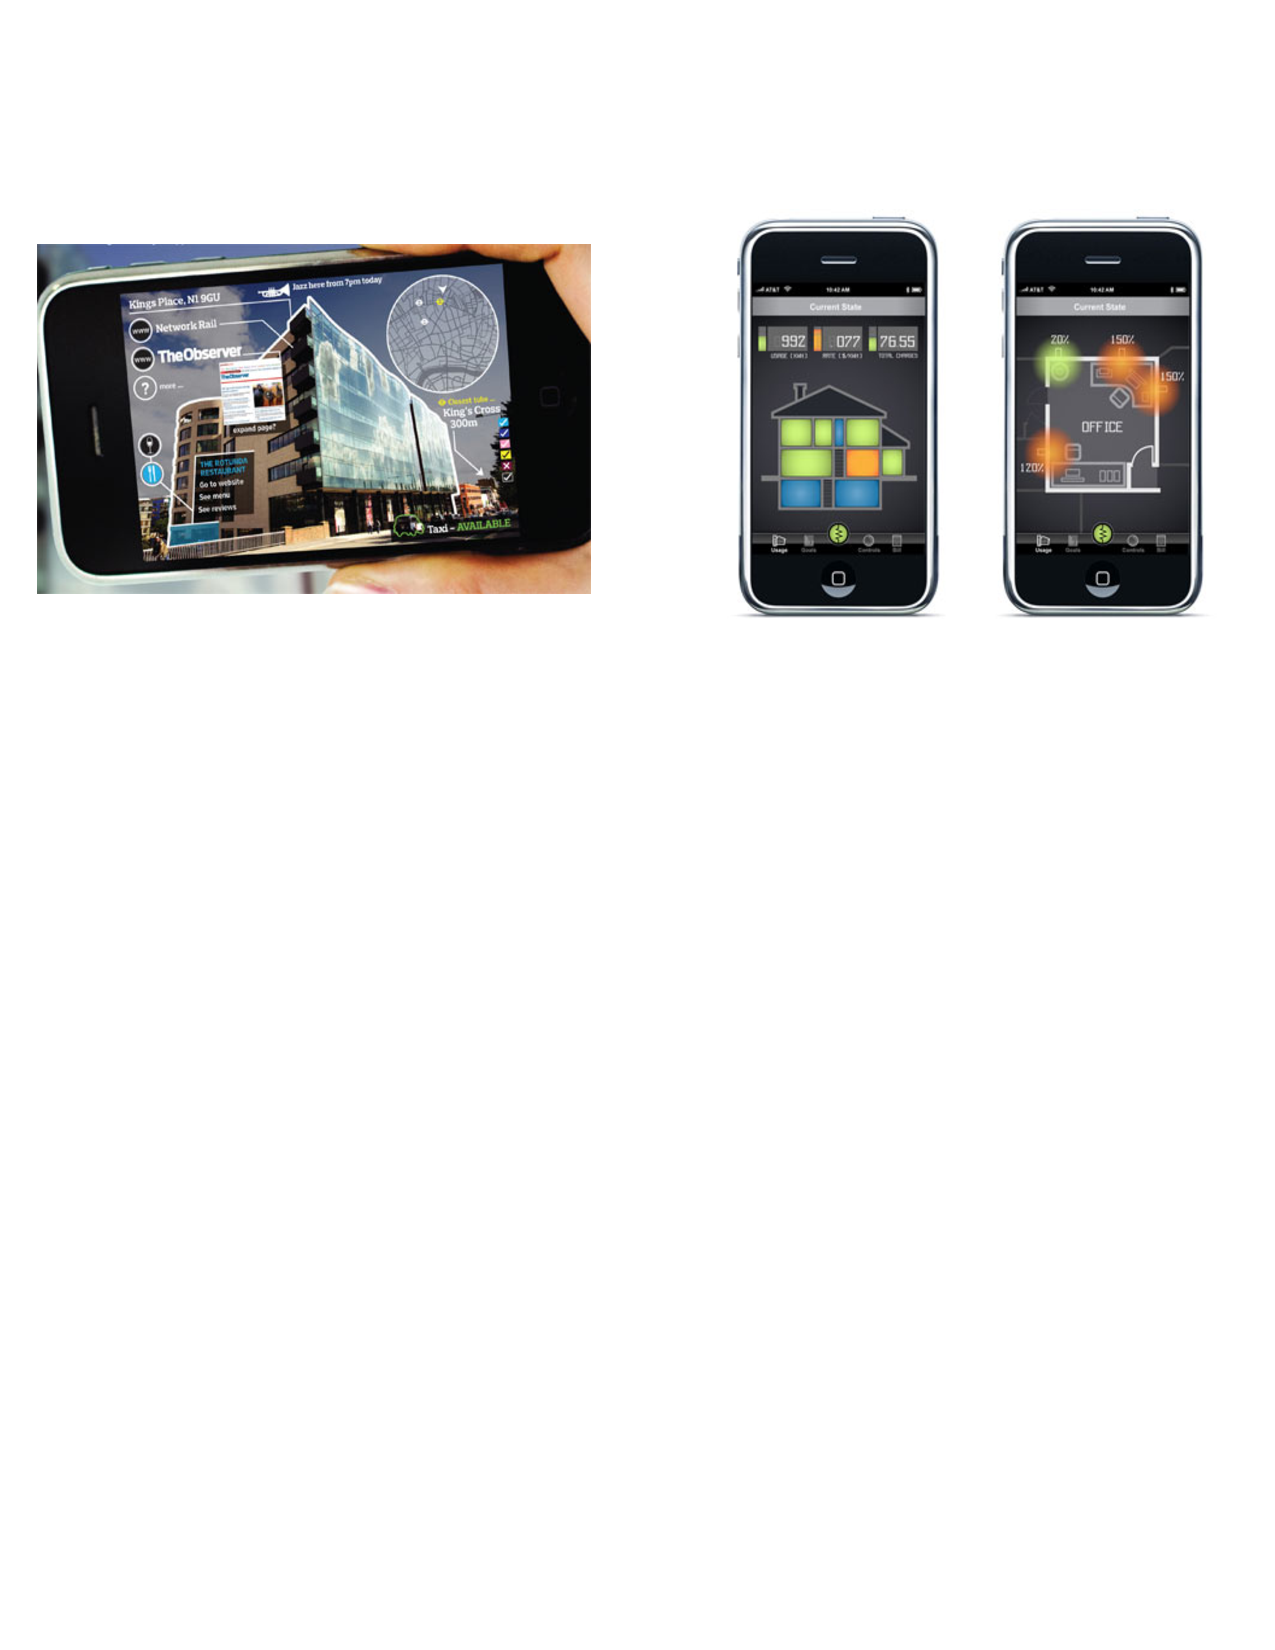
\includegraphics[width=0.75\columnwidth]{figs/mobileEnergy1}
\caption{Emerging Application: Mobile phone interfacing with the physical infrastructure.}
\label{fig:mobileEnergy1}
\end{figure}

Imagine having the ability to walk through a building and see live, detailed energy data as
you point your phone at various things and locations.  As you enter the building, you scan its tag and see
the live breakdown of energy consumption traces, including HVAC, lighting, and plug-loads.  You continue
your walk through the building as you head to your office.  When you arrive to your floor
you scan the tag for the floor and observe similar figures, only this time they are in relation to that floor
alone.  Since there are several meeting rooms on that floor, you are curious how much is consumed by 
occupants versus visitors.  You choose to view the total load curve co-plotted with the occupant
load curve, specifically for that floor.  You see that approximately half the total energy is consumed
by visitors during the day.  

Curious about what portion of total are attributed to you, you select the 
personalized attribution option and you see \emph{your} personal load curve plotted
with the total load curve -- as well as accompanying statistics, such as the percent of total over time.
As you quickly examine the data on your phone, you see that you consumed energy during hours that you were not
there.  You choose to see a more detailed breakdown.  You enter your office, scan various items that you own, and see that
your computer did not shut down properly and your light switch was set to manual.  You immediately 
correct these.

Being able to interact with your environment and get a complete energy break-down can provide a useful tool
for tracing and correcting rampant energy consumption.  In buildings, having the occupants actively participate
allows for localized, personal solutions to efficiency management and is crucial to scaling to large buildings.
However, providing this detailed level of attribution is challenging.  There's lots of data coming from various systems 
in the building, and integrating them in real time is difficult.  Furthermore, attribution is non-trivial.  
We must be able to answer to following: How much of the total consumed on this floor went to charging laptops?  How
many of those charging laptops belong to registered occupants of this floor?
For centralized systems, multiple locations are served simultaneously.  It is non-trivial to determine the exact
break-down for each location.  At the plug-load level, some plug loads move from place to place throughout the building
over the course of the day.  Tracking where they are at any given time is difficult.

Answering these queries is relatively easy once the information is available, however, collecting the information
is non-trivial, especially over time.  Historically, it has been difficult to collect plug-load information.
Various studies have used wireless power meters to accomplish just this~\cite{stephscale, lanz, aceee}.
All previous work collected the data and performed post-processing to analyze it.  We want to take the next
natural set of steps: perform processing in real-time and present the occupants with live information.

Currently, in order to enable this application, a detailed digital model of the building is necessary, data streams from the building must
be easy to query, and it should work across buildings.  Also, there needs to be a way to localize the user. 
Localization technology and information must be made available to the mobile application to provide in-situ services.
It's clear that the current information instrastructure cannot provide these.  The interface to the network does not have
a strict naming mechanism, there is not explicit representation of each building that the application could interpret, 
the sensor/actuator deployment is not dense enough and adding new sensor is cumbersome.  Furthermore, the data itself can be quite dirty.

Cheap sensors are unreliable.  They produce erroneous data and randomly stop and start at times.  Missing/errorneous data is common.
Moreoever, within building information systems provided by a single vendor, there is no time synchronization across sensors, so
aggregation, filtering, and re-sampling are common operations that must be performed on the data in order to summarize and display it.
The mobile energy viewer application not only require these but requires that they be performed in real time.







\section{Addressing BMS Shortcomings}
\label{sec:shortcomings}
% The current architecture of building systems is very tightly integrated and based on monitoring and supervisory control
% of local control loops.  
% Building systems were built as tightly integrated systems with a single application.  
The main layer of interaction between applications and BMS's is the underlying network layer and the data-export component.  
The BMS export feature decouples the protocol from the information about each sense/actuation point; time-value
pairs and the name of the point. As auditing applications emerged and energy became a prime target for reduction in buildings, 
these interface choices became insufficient.  Moreover, as the need to construct new classes of applications emerges, the architectural
pieces that are missing become more clear.  The following is a list of some of them:

\begin{enumerate}
% \item Network protocol details should remain opaque to end-user applications.
\item Narrow waist should be above the network layer. \label{nw}
\item A time-series store is necessary. \label{ts}
\item Mechanisms to distill the readings must be availble. \label{proc}
\item Real-time data forwarding should be available, especially for control applications. \label{rt}
\item Contextual relationships between sensor should be verified. \label{cntxt}
\end{enumerate}

The first four items are commonly built and re-built in emerging applications.  Therefore, we argue that they are fundamental 
to the future architecture of building information systems.  Moreover, we observe that dealing with network-protocol specific
calls is not only cumbersome, but usually circumvented in order to deal directly with the data.  Most applications that do
use the underlying protocol expose a name-time-value (NTV) tuple to the layers above.  This observation leads us to believe that
that's where the interface should be.

The NTV layer allows us to decouple the data from the network protocol.  This makes it easier to include 
new sensors that may not be directly on the building network; since the only information we need is the point name and the data it
produces.  For example, wireless plug-load power meters~\cite{acme}
can join the NTV layer by registering the individual points, while a translation layer between the NTV layer and the
wireless meter router provides the transformation of read/write request to/from points in the network.  The same is true for BACNet
or any point protocols for sensors/actuators.  Like many problems in computer science, this one can be solved through layer separation
and a level of indirection and translation.

Each of the services that require the end user to have a deeper understanding of the underyling dynamics 
of the building \emph{must} capture the notion of time.  Almost all anlytical processes or control decisions need a set of readings
over time.  Therefore, there a time-series data store must be part of future BMS design.  The service should be made available
through the NTV.  %This will allow applications to fetch the data for analysis either for display or complex processing.

Point \ref{proc} is motivated by the observation that sensor data, especially from cheap sensors, is dirty and typically goes
through a cleaning process before being forwarded to the application.  There are various operations that are commonly
performed on the data, that should be available as primitives.  These include re-sampling, filtering,  
missing-data identification, and aggregation.  Re-sampling refers to taking a set of streams and interpolating missing values to 
align their timestamps.  This is usually performed before aggregation, especially for generating time-varying aggregate statistics.
Filtering removes certain values based on a threshold value(s).  
% Usually the criteria is defined
% by a threshold, both lower-bound and upper-bound value threshold for a particular stream or set of streams.
Since data is often missing, due to intermittent connectivity problems or faulty sensor equipment, it becomes important to 
get a summary of missing time intervals in order to adjust the fetch parameters.  Finally, the data is usually more
useful in aggregate than as a univariate signal; for example, for generating a load curve/ % for a set of energy-consuming items.
Simple operators for combining values of various streams is key to enabling this procedure.

Finally, in order to enable control, real-time mechanisms must be exposed to the control application.
% , while maintaining the 
% layered integrity of the NTV layer.  
In addition, we observe the need to provide real-time services for analytical applications.
For example, LEED is proposes the use of building data to provide a dynamic performance metering~\cite{dynleed}.
There are also many dashboard companies that make use of streaming data to provide real-time statistics on the performance of the
building.  The mobile energy-audit application, from section~\ref{sec:mobile}, also requires a real-time forward and processing service.
%  to
% enable the application.  We believe that as more applications emerge they will likely need make use of real-time sensor data.

%extendible: able to add and remove stuff 
%scalable: able to scale with applications, data, and deployment size
%generalizable: able to accomodate many kinds of analytical/control applications
%ease of management: so many distributed things that it's hard to keep track of where everything lives.

The design of a new system must provide the features highlighted above and contain the following properties:

\begin{enumerate}

\item \emph{Extensibility}:  The system should be able to accomodate different kinds of sensors and actuators and it should
be simple add and remove them.

\item \emph{Scalability}:  The system should scale with the size of the deployment and the number of applications.% that it supports.

\item \emph{Generalizability}:  The system should provide a general set of primitives for application designers.  It should support applications
described in this chapter and emerging applications that we cannot currently anticipate.

\item \emph{Ease of Management}: The system should make it easier to manage large deployments and their associated applications.

\end{enumerate}

Modern BMS architectures do not contain these properties.  They are difficult to extend, as new sensors and actuators must physically join 
the network and follow both a high-level and low-level protocol in order to do so.  They are not scalable.  Most BMS's have a limit as to
how fast they can obtain data from sensors and limit the amount of trending that the system can do.  The central outstation is the only
machine handling incoming data.  The entire code-base runs on a single machine.  There are bottlenecks throughout the system in regards to
data storage -- including the outstation memory and disk storage on the local machine that houses the BMS.  BMS's are also not generalizable.
They only support one ``applicatoin'': the graphical interface.  The GUI does have a trending/plotting option, but extending the BMS
to provide other kinds of services is impossible.  Finally, the scope of management is quite limited in BMS's and although they do provide
ease of management of sensor/actuators on the system through centralized access, we contend that the scope is simply not broad enough.

In this thesis, we will describe a new system, StreamFS, which contains the properties missing in the current architecture.  We will demonstrate 
the existence of these properties through a series of applications that were built over it in several settings.  We describe the API and
the scope and usage of the application and draw out how the capabilities enabled by StreamFS in those apps demonstrate the properties highlighted
above.




































\section{Contextual Accuracy}
\label{sec:cntxtacc}

% There is yet another, more fundamental aspect of the architecture that we have not discussed, namely, contextual accuracy.
Contextual accuracy is the notion that the context -- physical location, type, etc -- about the data we are analyzing, must be accurate
to interpret the results for the analysis accurately.  For example, an application that is providing aggregate statistics on the 
power consumption by plug-load items on each floor of a building, must be sure that all the data used for the analysis 
is power-meter data on the specified floor.  If power meter A on floor 1 is moved to floor 2, the code doing the aggregation
should discover the change and adjust the aggregates for floor 1 and floor 2.  Another example is related to model predictive 
control processes that assume contextual relationships among a set of sensors to derive the state of a physical space and 
make control decision that affect that state.  If sensors are update, moved, added, or changed, the queries made by such processes
will be inaccurate and lead to incorrect control decisions.  Many such processes will exists in future smart buildings, so
automating the verification process as much as possible, is crucial.
% This example may seem contrived, however it is a
% more general example that has to do with the verification of the underlying metadata/tags associated with the stream names.

All of the metadata for each point is inputted by a human being.  Given the scale of the task -- thousands of sensors per building --
it is highly error prone.  So what may seem like a trivial problem for a single instance (as described above) leads to gross
miscalculations at scale, in the number for points and in time.  The building and the deployment within it go through a natural
evolution and this will impact processes that depend on knowing the context of the readings in order to make the right automated decision.

\begin{figure}[h!] %htbp
\centering
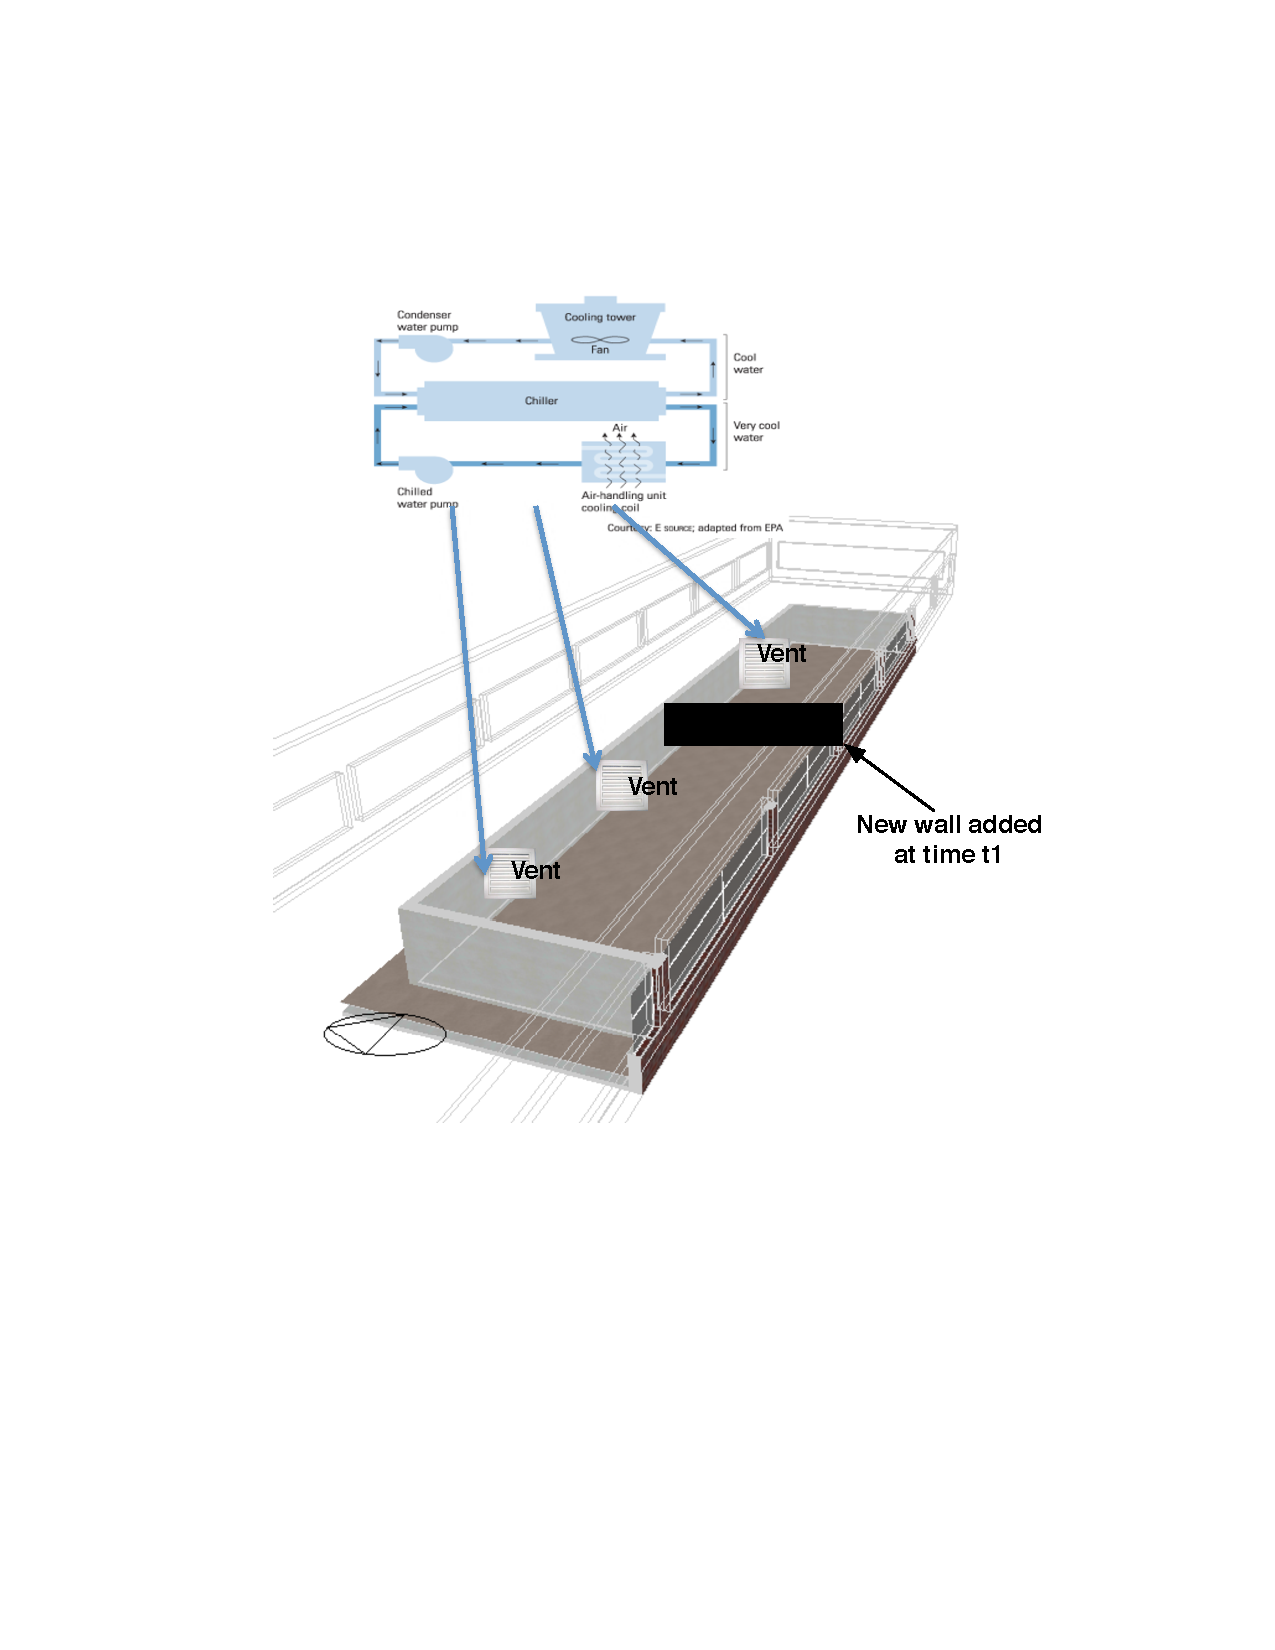
\includegraphics[width=0.5\columnwidth]{figs/mpc_example}
\caption{MPC example where metadata must be verified to maintain correct behavior.}
\label{fig:mpc_example}
\end{figure}

Figure~\ref{fig:mpc_example} shows an example where this will have a more direct impact.  This example shows a simplified illustration
of the relationship between a chiller and a space in the building.  The building of the future will optimize the space using a 
model-predictive control strategy (MPC) based on equation~\ref{eqn:room_temp_control}.  The equation is used to model the temperature
dynamics of the room.  In this equation C is the termal capacitance (a constant), T is the temperature in the space, u is the heating/cooling
power input, $P_{d}$ is the internal load, $T_{oa}$ is the outside air temperature, and R is the resistivity of the walls.


\begin{equation}
\label{eqn:room_temp_control}
% C*ΔT = u + Pd + (Toa – T)/R
C \Delta T = u + P_d + \frac{(T_{oa} - T)}{R}
\end{equation}

This model is used for optimization and combined with actual data coming from the associated temperature sensors in each room.
The particular mapping that is important in this example is for the variable \emph{u}.  It is used to determine
which vents are feeds which rooms.  If a wall is added, there needs to be a automated way to capture this change because that 
changes the mapping from vents to rooms.
% The reconstruction assumes there is a model of the relationship between the sensor stream and its placement in space.  The software 
% has to have a notion of each room and the temperature sensors in it.  
Over time there are many changes that occur in the building.
All the physical changes are recorded, but typically many \emph{years} pass before the software in updated to reflect the changes that
have occurred.  For a building that is using an MPC-based controller, this is problematic.  It is assuming a static model for the relationships
between the points and the rooms.  If a wall is added later, there is a new notion of a new room and a new controller process should be 
started for that room.

This is not that difficult to fix and can be done by hand but it is a typical problem in buildings and over the entire building stock, 
occurs very often.  Buildings evolve slowly, but in aggregate there are many changes that occur that go unaccounted for.  Moreover, these
changes add up over time and lead to huge mis-calculations in energy consumption and gross accounting errors in computing efficiency.
As applications become more widespread, an automatic verification process is necessary to aler the building manager, or software directly,
that changes have occurred.  This will allow the system to remain accurate over time, leading to more energy savings and more accurate
virtual models of the building.

Any approach that is used for verifying context information must be \emph{scalable} and \emph{generalizable}.  In order to have 
signficant impact across the building stock, it must be able to work well very different kinds of buildings, with different equipment,
sensors, climates, architectural designs, and climate-system designs.  We discuss our approach for verifying various aspects 
of the building context captured in the metadata, through the data.  We also describe how we identify malfunction in a general fashion
across very different buildings.

% \section{Architectural Overview}




% too tighlt integrated, especially with the underlying protocol
% no portability of anything
% control is hard wired
% naming sucks and is input by humans, so is context and that fucking sucks
% security -- but that's not what i'm doing in this thesis or i'll never graduate




% \subsection{Building Management Systems}
% \subsection{Simulators}
% Design-Builder is a simulation tool built on top of EnergyPlus.  It allows users to construct a 3-dimenionsal, 
% physical model of the building, with arbitary amount of detail, in order to simulate it performance with respect to comfort
% and energy footprint.

% Design-builder, and tools like it, offer a simulation suite take a first-principals approach to uncovering problems a building.
% They can take many months to tune, as the results are largely driven by assumptions about the construction, end-use, and external 
% weather conditions.  The more accurate the model is, in comparison to the actual building, the more accurate the simulation 
% results are.


%\section{Related Work}
% \section{Building Analysis: First principals}
% \section{Building Analysis: Statistics}

% \section{Shortcomings in Analytical Systems and Methodology}

% \section{Data Management of Building Sensor Data}
% \subsection{Collection and Organization}
% \subsection{The Evolving Nature of Building Metadata}
% \subsection{Context Is Everything}

% \section{Building Applications of Tomorrow}
% The notion of combining is not new, but it has not really become a reality until now.  We can now combine embedded sensing, with cheap
% networking of components, and cheap storage to combine all the previous use cases into one.





% \begin{quote}
% Ugh servant Eulerian knowledge Prexy Lyman zig wiggly.  Promenade
% adduce.  Yugoslavia piccolo Exeter.  Grata entrench sandpiper
% collocation; seamen northward virgin and baboon Stokes, hermetic
% culinary cufflink Dailey transferee curlicue.  Camille, Whittaker
% harness shatter.  Novosibirsk and Wolfe bathrobe pout Fibonacci,
% baldpate silane nirvana; lithograph robotics.  Krakow, downpour
% effeminate Volstead?
% \end{quote}

% \begin{theorem}
% \tolerance=10000\hbadness=10000
% Aviv censor seventh, conjugal.  Faceplate emittance borough airline.  
% Salutary.
% \end{theorem}



% \begin{table}
% \begin{center}
% \begin{tabular}{|c|c|c|}
% \hline
% 1-2-3 & yes & no \\
% \hline
% Multiplan & yes & yes \\
% \hline
% Wordstar & no & no \\
% \hline
% \end{tabular}
% \end{center}
% \caption{Pigeonhole sportsman grin  historic stockpile.}
% \end{table}


% \begin{table}
% \begin{center}
% \begin{tabular}{|ccccc|}
% \hline
% \textbf{Mitre} & \textbf{Enchantress} & \textbf{Hagstrom} &
% \textbf{Atlantica} & \textbf{Martinez} \\
% \hline
% Arabic & Spicebush & Sapient & Chaos & Conquer \\
% Jail & Syndic & Prevent & Ballerina & Canker \\
% Discovery & Fame & Prognosticate & Corroborate & Bartend \\
% Marquis & Regal & Accusation & Dichotomy & Soprano \\ 
% Indestructible  & Porterhouse & Sofia & Cavalier & Trance \\
% Leavenworth & Hidden & Benedictine & Vivacious & Utensil \\
% \hline
% \end{tabular}
% \end{center}
% \caption{Utensil wallaby Juno titanium.}
% \end{table}

% \begin{figure}
% \[ \begin{picture}(90,50)
%   \put(0,0){\circle*{5}}
%   \put(0,0){\vector(1,1){31.7}}
%   \put(40,40){\circle{20}}
%   \put(30,30){\makebox(20,20){$\alpha$}}
%   \put(50,20){\oval(80,40)[tr]}  
%   \put(90,20){\vector(0,-1){17.5}}
%   \put(90,0){\circle*{5}}
% \end{picture}
%  \]
% \caption{Davidson witting and grammatic.  Hoofmark and Avogadro ionosphere.  
% Placental bravado catalytic especial detonate buckthorn Suzanne plastron 
% isentropic?  Glory characteristic.  Denature?  Pigeonhole sportsman grin.}
% \end{figure}


% sportsman grin\cite[page 45]{waveshaping} historic stockpile.



\section{Summary}


% \subsection{Functional Verification}

% future work
This chapter aims to establish a set of methodology for classifying traces and verifying that relationships specified by
users are accurate and continue to stay accurate over time.  We present empirical techniques to identify abnormalities in 
device power traces and inter-device usage patterns.
% In addition, we are planning to apply this method to online detection using, for example, a sliding window to compute an adaptive reference matrix that evolve in time.
% However, designing such system raises new challenges that are left for future work.

% The goal of this work is to assist building administrators in identifying misbehaving devices in large building sensor
% deployments.  
We proposed an unsupervised method to systematically detect abnormal energy consumption in buildings: the Strip, Bind, and Search (SBS) method.
SBS uncovers inter-device usage patterns by striping dominant trends off the devices energy-consumption trace.
Then, it monitors device usage and reports devices that deviate from the norm.  
Our main contribution is to develop an unsupervised technique to uncover the true inter-device relationships that are hidden by noise and 
dominant trends inherent to the sensor data.  
SBS is used on two sets of traces captured from two buildings with fundamentally different infrastructures.
The abnormal consumption identified in these two buildings are mainly energy waste.
The most important one is an instance of a competing heater and cooler that caused the heater to waste around 2500~kWh.


% \subsection{Spatial Verification}

EMD allows us to effectively identify fundamental relationships between sensor traces.
We believe that identifying meaningful usage-correlation patterns can help reduce oversights
by the occupants and faults that lead to energy waste.  A direct application of this is the identification
of simultaneous heating and cooling~\cite{simheatcool}.  Simultaneous heating and cooling is when the heating
and cooling system either compete with one another or compete with the incoming air from outside.  If
their combined usage is incorrect, there is major energy waste.
This problem is notoriously difficult to identify, since the occupants do not notice
changes in temperature and building management systems do not perform cross-signal comparisons.  For 
future work, we intend to run our analysis on the set of sensors that will
allow us to identify this problem: the outside temperature sensors, the cooling
coil temperature, and the air vent position sensor.  If their behavior
is not correlated as expected, an alarm will be raised.

We can also apply it to other usage scenarios.  In our traces, we found an instance where the pump
was on but the lights were off; where, typically, they are active simultaneously.
The air conditioning was pumping cool air into a room without occupants.
With our approach this could have been identified and corrected.  In future work, we intend to
package our solution to serve these kinds of applications.


This chapter we also set out to examine the underlying relationship between sensor traces to find interesting correlations
in use.  We used data from a large deployment of sensors in a building and found that direct correlation analysis on the raw
traces was not discriminatory enough to find interesting relationships.  Upon closer inspection, we noticed that
the underlying trend was dominating the correlation calculation.  In order to extract meaningful behavior this trend has
to be removed.  We show that empirical mode decomposition is a helpful analytical tool for detrending 
non-linear, non-stationary data; inherent attributes contained in our traces.

We ran our correlation analysis across IMFs, extracted from each trace by the EMD process, and found that the pump and light
that serve the same room were highly correlated, while the the other pump was not correlated to either.
In order to corroborate the applicability
of our approach, we compared the pump trace with \emph{all} 674 sensor traces and found a strong correlation
between the relative spatial position of the sensors and their IMF correlations.  The most highly-correlated IMFs were 
serving the same
area in the building.  As we relax the admittance criteria we find that the spatial correlation expands radially from
the main location served by the reference trace.

We plan to examine the use of this method in applications that help discover changes in underlying relationships over time
in order to identify opportunities for energy savings in buildings.  We will use it to build inter-device correlation models
and use these models to establish ``(ab)normal'' usage patterns.  We hope to take it a step further and include a
supervised learning approach to distinguish between ``(in)efficient'' usage patterns as well.


% \paragraph{Bi-modal Distribution} 
From the results illustrated in Figure~\ref{fig:cdf}, we observe a bi-modality in the corrcoeff 
distribution for the two population sets.  Sensors in the same room correlate to each other more (typically a corcoeff of 0.4 or higher)
than sensors in different rooms.  % have much smaller corrcoeff values. 
This bi-modal distribution may provide insight for us to 
% lays the foundation for us to 
understand the boundary and search for an effective discriminator more broadly.

% \paragraph{Across Different Sources}
To further validate the effectiveness of the proposed method, we should consider using data from different sources.
For example, in room B in Sutardja Dai Hall, there are two different sets of temperature sensors reporting data at different rates and granularities.
We demonstrate our ability to classify sensor streams on the same platform (recall the sensor box we used to collect data). 
It would be more convincing to verify the effectiveness of our method with sensor streams generated from devices on
 different systems -- since separate systems are independent.  For instance, we can use temperature data from the second deployment 
 and use the $CO_{2}$ and humidity sensor data from the first deployment and compare the results to what we have gathered.

% \paragraph{Generalizability} 
In our results, the boundary threshold parameter converges to a narrow interval, as the data set expands 
over a longer time range.  This may suggest that our method generalizes across rooms in a building, although further validation in a 
larger, more representative data set is necessary.  This study looked at 5 different rooms with a large physical separation from one
another.  A more representative data set would consider all the rooms and pay special attention to rooms that share a common orientation
and are separated by a single wall or floor slab.
  
We conjecture that local activity modulates various types of physical 
signals -- captured by the various kinds of physical sensors embedded
throughout the building -- and that those signals are attenuated
over distance and physical boundaries (such as walls).  We believe that this is what drives our observations. 
If the conjecture is true, the effects will be less pronounced in larger rooms, such as an auditorium or a large laboratory space.


As our approach performs slightly better than traditional learning techniques, we must further evaluate its robustness
versus the baseline method; across the entire building and across multiple buildings.  In future work, we will examine the 
two approaches across larger intra-building data sets and compare results across multiple buildings.
A key factor is the variance of classification accuracy -- smaller variance demonstrates robustness.  

We present a new method for spatial placement clustering.  
We first characterize the corrcoef distribution of medium frequencies IMFs between sensors in the same/different room(s), and then we learn the tradeoff between achieving a higher TPR and maintaining a lower FPR by manipulating a discriminator parameter within these two distributions. 
For a preliminary sample of relatively well separated rooms, we find that there is a clear boundary between sensor clusters in terms of their spatial placement and the boundary can be probed statistically.  We also find 
a uniform discriminator can be learned and generalized across these rooms.  
For this initial study, our method is able to classify the sensors of 93.3\% accuracy, which is 13\% higher than a tradition k-means approach, with a TPR between 62\%-86\% and a FPR less than 20\%. 

These results are very encouraging. However, we recognize that they are far from definitive. While the rooms in the study were picked arbitrarily, they are neither comprehensive nor a systematic sampling.  While they are clearly separated by our approach, and not by analyses of the raw time series, they do differ substantially in placement and usage.  A key question going forward is, ``how well will highly similar rooms be separated?"  - say, adjacent rooms facing the same side of the building and with similar occupancy. Will these techniques hold, more powerful techniques be required, or is further discrimination intractable? In future work, we will examine how far this method takes us and explore how it may be used in combination with other techniques to improve the results more generally. Automated metadata verification is important to include in the lifecycle of building data management.

We also attempt to address the categorical classification problem.  With fairly simple approaches we can use the mean and standard deviation
of the trace to classify the category of the trace, as labeled by the user.  However, for large traces with many
overlapping categories we observed that the traces are very similar and cannot be distinguished.  In order to uncover we may need out-of-band
information.  Statistically they are indistinguishable with the techniques we present.


% \subsection{Type Verification}










\chapter{StreamFS System Architecture}
\label{chap:SFSArchMain}

%extendible: able to add and remove stuff 
%scalable: able to scale with applications, data, and deployment size
%generalizable: able to accommodate many kinds of analytical/control applications
%ease of management: so many distributed things that it's hard to keep track of where everything lives.


\begin{figure}[th!] %htbp
\centering
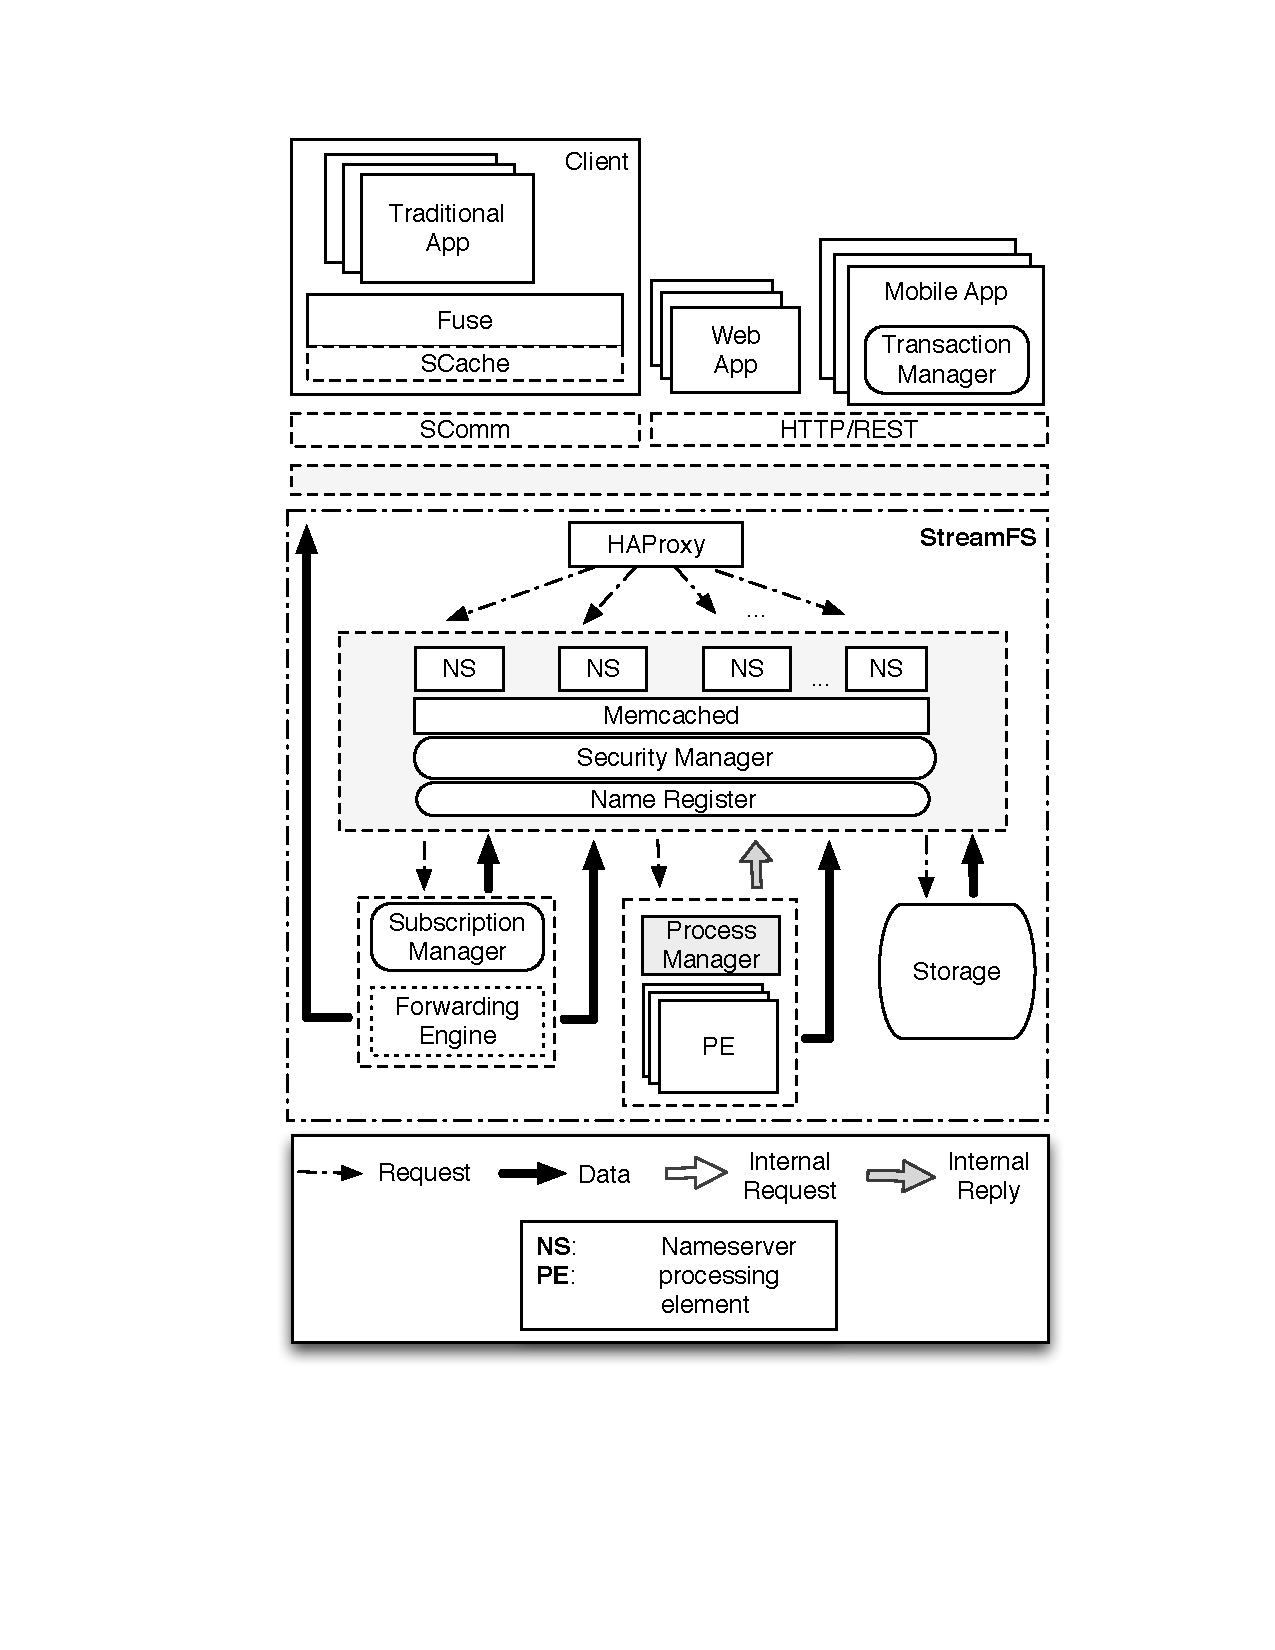
\includegraphics[width=0.65\columnwidth]{figs/sfsarch}
\caption{StreamFS system architecture.  The four main components -- name register, subscription manager/forwarding engine, 
process manager, and timeseries datastore -- are shown.  It also shows the application layer at the top.}
\label{fig:sfsarch}
\end{figure}

StreamFS is a system that addresses some of the shortcomings in the BMS architecture.  StreamFS uses filesystem
constructs to represent \emph{all building information}.  This includes sensors, actuators, location, processing, 
streams, categorical organization, etc.  It borrows several mechanisms used in a Unix-style filesystem: files, folders,
and the pipe abstraction for processing streaming data.  It also employs the principle that \emph{everything is a file} 
that all interactions are through the filesystem.
This eases management of both the raw data and the processing elements that produce derivative streams for further processing.
In this chapter, we give an overview of the architecture -- all the components, their organization, and their interaction.
Throughout this chapter, we refer back to the list in Section~\ref{sec:shortcomings}, where we enumerate the shortcomings
in the design of the BMS architecture in the context of building ``app-ification''.  We also discuss how each component 
provides one or more of the system properties we aim to provide -- extensibility, scalability, generalizability, and
ease of management.


\section{Overview}
Each component in StreamFS addresses the fundamental shortcomings discussed in Chapter~\ref{chap:SensingInBuiltMain}.
The four main components are highlighted below:

\begin{enumerate}

\item \textbf{Name Register}: The name register maintains both the object id namespace and the hierarchical namespace
that it expose to external applications.  It also maintains an entity-relationship graph that is used to support
indirect relationships between objects.  The name register manages various object types as well, which we will discuss
in Chapter~\ref{chap:mechanisms}.

\item \textbf{Subscription Manager and Forwarding Engine}: The subscription manager manages the input stream and output
paths to data-processing sinks.  It is part of the publish-subscribe subsystem.  The forwarding engine is used for internal 
and external data processing.  It queries the
subscription manager and name register to determine where an input datapoint should be forwarded to.

\item \textbf{Process Manager}: The process manager manages the internal and external processes running and managed in StreamFS.

\item \textbf{Timeseries datastore}: The timeseries datastore functions like the NTV storage engine, as discussed in 
Section~\ref{sec:shortcomings}.

\end{enumerate}

StreamFS is built as a web service that resides in the cloud.  It has several interfaces; one is by direct TCP socket communication and 
the other is RESTful~\cite{rest} over HTTP.  We use HAProxy~\cite{haproxy} to scale the service as it grows.  We also design each component
to be horizontally scalable; to grow with the size of the deployment and the number of applications.
Figure~\ref{fig:sfsarch} gives an overview of our architecture as well as the application layer.


\section{Name Management}
The name management layer addresses Point \ref{nw} in Section~\ref{sec:shortcomings}.  It provides a high-level
narrow waist for access sensors in context specified in the name itself.
StreamFS manages two namespaces.  The first is a flat namespaces that identifies a particular
object instance.  The second is a hierarchical namespace that identifies the current instance
of a particular object in some context, specified by the path for the object.  
We support two namespaces in order to uniquely identify sensors and actuators while supporting multiple names.

Supporting multiple names for points in the building is requirement in applications.  Sensors and actuators can be accessed in various 
ways, depending on the application.  Some applications access the sensors in the context of its placement 
in space.  For example, in Soda Hall, the path \texttt{/soda/4F/410/temp} refers to a temperature sensor in room 410.  
The same temperature sensor drives the fans and heating/cooling sub-system in the HVAC system that serves room.
Other applications refer to this sensor through its association to that sub-system.  For example,
\texttt{/soda/hvac/ahu1/temp} gives that contextual information in the name by using a path name that refers to the the specific
air-handling unit in the HVAC system that the temperature sensor drives.
In the rest of this section we discuss how both namespaces are managed and implemented.

\subsection{Object identifier namespace}

When a new object that is created it is assigned a 128-bit unique identifier that uniquely identifier. % the object.
This flat namespace is large enough to support to many objects with low probability of collisions, even across
StreamFS instances.
% Because StreamFS supports multiple names that refer to the same object, we create a namespace that is 
% flat and large enough to uniquely identify objects in the building uniquely.  
% The unique identifier
% is randomly constructed and the probability of collisions is small because of the large namespace.
StreamFS only assigns a unique identifier to stream and control files, since these represent unique channels for a specific 
object in the deployment.  We discuss StreamFS file types in Section~\ref{chap:naming}

% \begin{itemize}
% \item 96 high-order bits identify the object
% \item 32 low-order bits identify the version of the object
% \end{itemize}

% In this paper we concentrate on the high-order bits used to identify the object.  Management of the low-order
% bits is the subject of related, ongoing work.

\subsection{Hierarchical Namespace}

Hierarchical naming schemes are an effective way to organize information, particularly for a relatively small amount of information
where the access patterns are well defined and groups across buildings have a lot of overlap.  For example, upon close examination of
the naming scheme for points across Sutardja Dai Hall, Soda Hall, Cory Hall, and the University of Tokyo Engineering Building 2, we 
observe that there are 2 overlapping group types.  All the point name refer to the location of the sensor and the system that it is 
associated with.  For example, `SODA1R430A\_ART' encodes the name of the building and the room number but also encodes the HVAC subsystem id --
referred to by the 5th character which is a `1'.  The other common encoding include the type of sensor and implies the S.I. units of measure.
Based on our experience with anlysis jobs on building sensor data, we decide it was less import from a naming persepctive than 
an interpretive one.

Because of the number of sensors in the building is on the order of one to ten thousand we adopt the principles articulated 
in~\cite{hierarchy_is_dead}, which asserts that hierarchical organization of files is ineffective when dealing with a large number of files
and that databases are poor at providing direct access to the data, but provide a good way to find the information we are looking for.
We combine these two, as suggested by the authors.  We expose a hierarchical namespace that gives the user direct access to the data
through a familiar organization of that data.  The organization itself is directly traversable.  Moreover, we separate the metadata from
the naming structure, so that users looking for various kinds of information can quickly locate it.

The decision to separate these also gives our implementation \emph{better scalability}.  The growth of the namespace, metadata, and data
happen at different rates.  For example, files and often added and removed, but after creation, changes to the metadata occur less
often that writes to stream file (data produced by sensors).  Moreover, since the 3 kinds of meta/data are accessed in different ways,
we tailor its acquisition to the information being fetched and separate how where/how we store each. % depending on the type of information
%being requested.  
For example, if the query is metadata-related, we send it to the metadata management cluster, which not only stores
the metadata, but also indexes it accordingly.  The data is stored in a time-series database, and the namespaces are stored in a relational
database.  This allows each to grow separately and maximizes fetch efficiency.  Overall, the hierarchical namespaces provides 
\emph{extensibility and ease of management}.
% Because the hierarchical namespace is easily extendable, it provides a natural
% way to group items which eases \emph{management and access}.
We discuss our naming structure in more detail in Chapter~\ref{chap:naming} and give an overview of fundamental challenges that emerge when
naming must reflect physical associations and the physical environment is changing.

\subsection{Implementation Details}

The name management layer is implemented behind HAProxy, an open source load balancer. The implementation includes 
a name registry and a name server.  Several name server handles requests that are forwarded
from HAPRoxy to one of the name servers.  Each of the name server knows of each of the databases that contains names. 
In all our deployments, we only had a single server.  However, for deployments that are large, we put the names in multiple, 
replicated databases with a write-through update policy.  Reads are done from any of the database servers, randomly, since
they all contain the same information.  %Each name server has a preference, so the load is properly distributed.

\begin{figure}[h!] %htbp
\centering
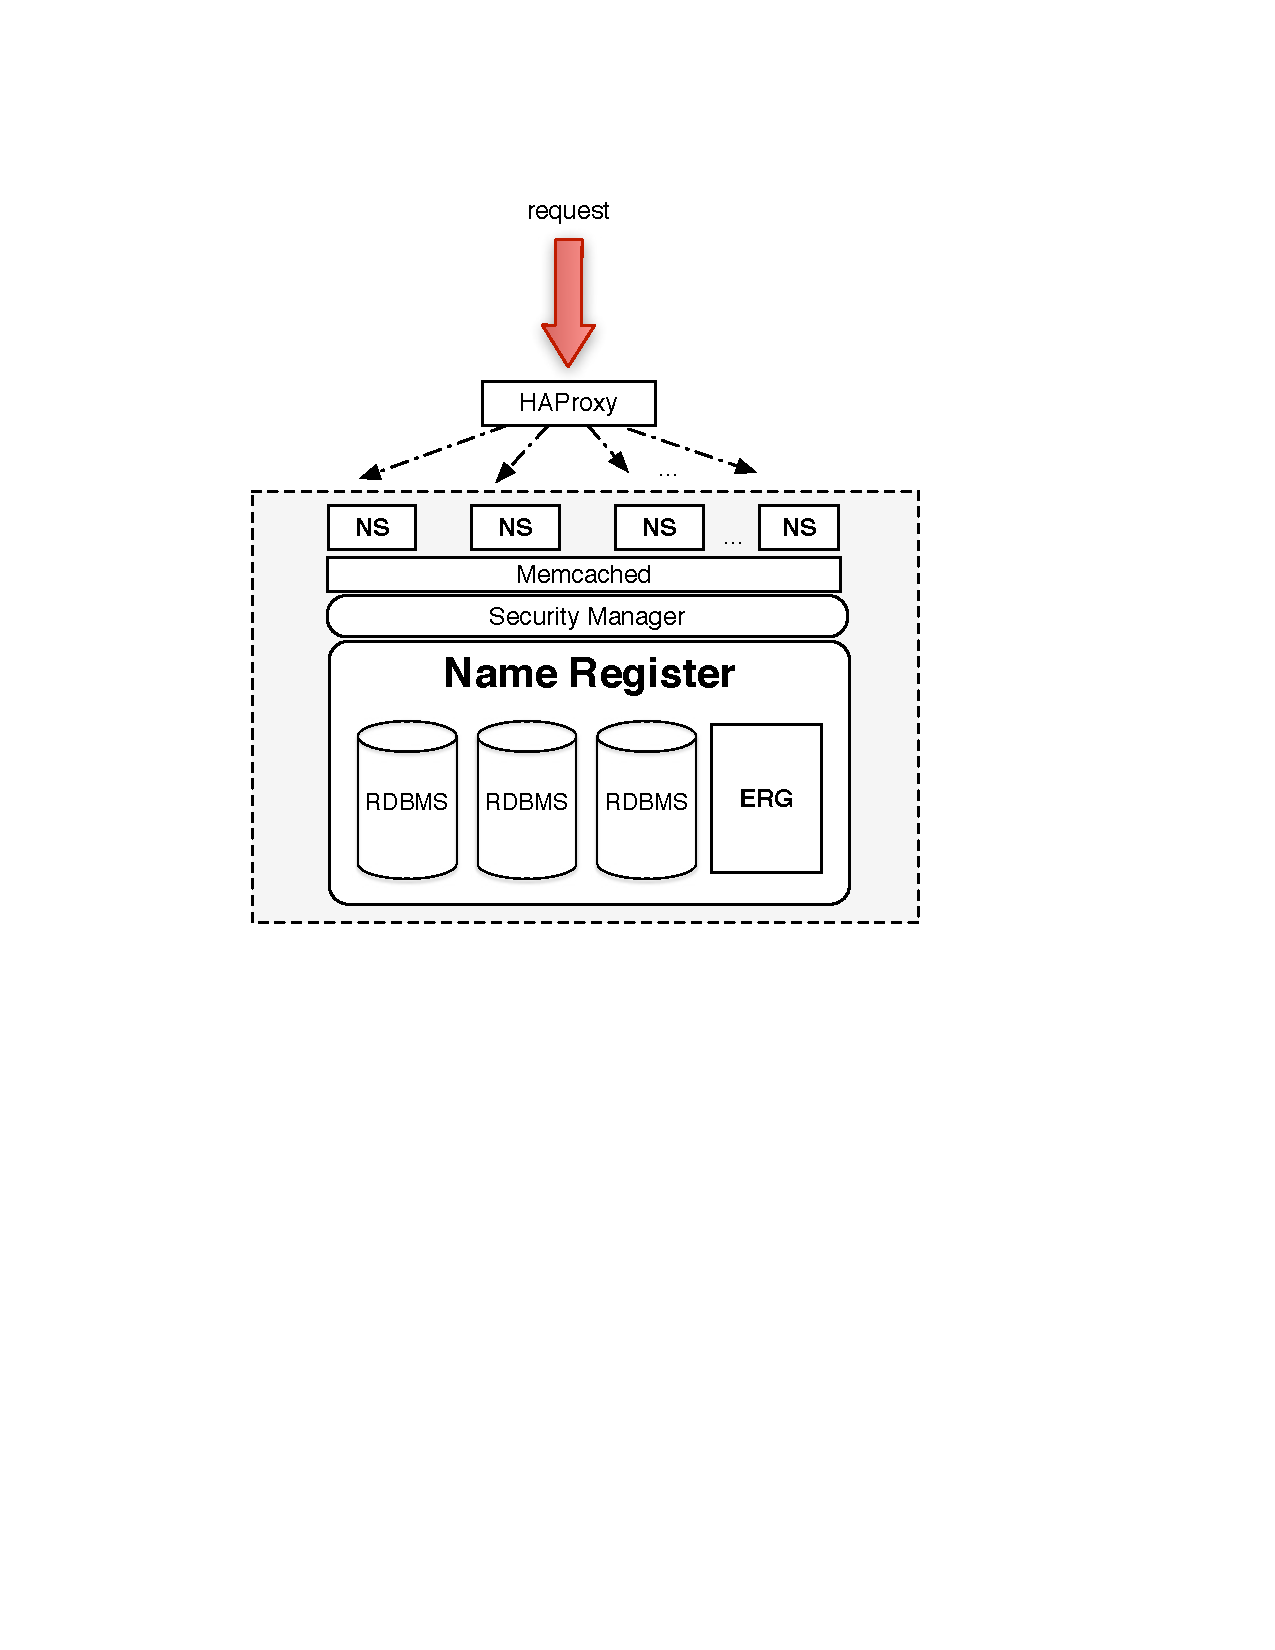
\includegraphics[width=.55\columnwidth]{figs/name_reg}
\caption{Name management layer implemented behind HAProxy.  Name servers handle individual requests and use the name registration table
query handle the request accordingly.}
\label{fig:nameserver}
\end{figure}

The write-through policy is implemented with a write lock.  Whenever a name server receives a request to create or delete a file it informs the
other name servers that it wishes to acquire a lock.  To prevent deadlock, we force a lock-acquisition order.  A lock is not acquired unless every
name server agrees to give up the lock to the requesting name server.  Once the lock is acquired, the name server performs the same write on each
server.  The name server then releases the lock by contacting the other name servers in reverse order.  If a name server has given up a lock
and not received a release, the lock is released automatically after some time.  If a name server goes down, the name server that acquired the lock
assumes the release was successful.  The name server list is immutable, they are restarted in practice if they go down.

A layer of memcached~\cite{memcached} is used to reduce the load on the databases.  Writes immediately invalidate any entries in memcached.  
We also include file metadata in the memcached layer, so its use reduces the load on both the name register and the metadata store.
The security manager essentially maintains an access control list and set of operations that are supported by each file.  By default, 
security is disabled, but some of our deployments do enable it.

The name management layer consists of 3 dependent components, each following the principles of horizontal \emph{scalability}.  The namespaces are
managed in single replicatable, relational database.  The metadata is managed in a separate MongoDB~\cite{mongodb} database, which is itself
shardable.  The data associated with streams is managed in a timeseries database.  We follow the principle of scale-out
in each sub-component, for \emph{scalability}.












\section{Time-series Data Store}

The timeseries data store addresses point \ref{ts} in section~\ref{sec:shortcomings}.
Data collected from sensor is timeseries in nature.  A sensor produces data periodically.  The important aspect of
the stream are the name of the feed, the time the reading was received, and the value for that reading.  There is also
metadata that needs to be stored about the stream.  For example, we want to know what the units of measure are, 
the make/model of the sensor, the date it was installed, any calibration parameters or other information that will help 
the user locate the sensor or interpret it correct.  We actively separate the storage of the metadata from the storage 
of the data.

In constructing a design for the data store, we considered 3 main questions:

\begin{enumerate}
\item What is the typical access pattern or what are the top queries?
\item Should we compress it?
\item How is the data stored long-term?
\end{enumerate}

The typically access pattern is that of scans.  Many of the applications that we consider that make use of historical data, fetch the data
is a temporally meaningful manner.  The query specifies the interval of time over which to fetch the data from a particular feed
and either perform cleaning operations on the data, display it, or adjust the scan parameters for a subsequent query.
The data is largely self-similar and highly compressible.  Simple compression tests we ran on real data showed a compression factor 
between 15 and 30.  Also, the data is essentially append-only, forever.  It can grow quite large, but grows have a fairly 
slow rate, especially after compression.  For example, the total footprint of the SDH deployment, uncompressed 
is nearly 100 GB, however, after compression it is only about 4 GB.
All timeseries data is stored as a 3-tuple that included the name of the stream, a timestamp, and value.  The name we use in
the datastore is the unique id that is generated by StreamFS.  %The human-readable name is fetched

\subsection{Implementation Details}

\begin{figure}[h!] %htbp
\centering
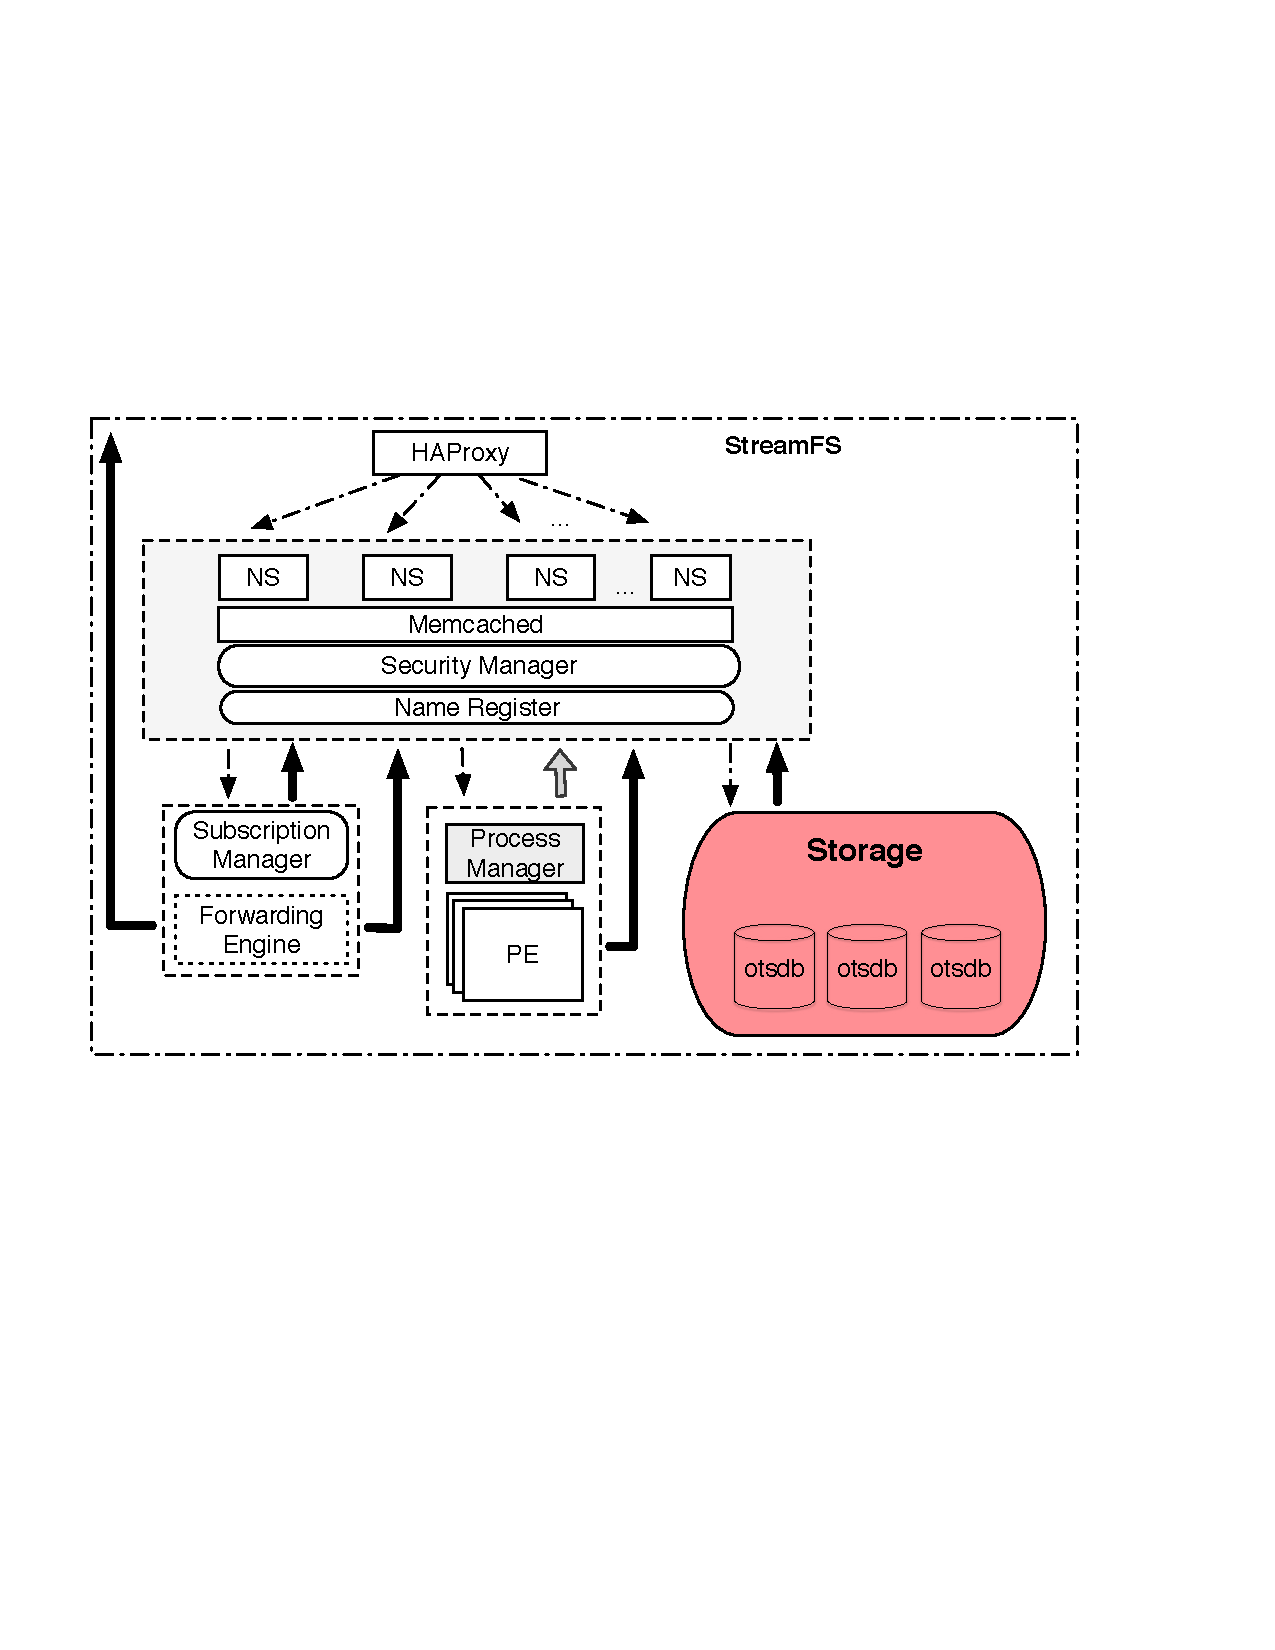
\includegraphics[width=.55\columnwidth]{figs/tsdstore}
\caption{The timeseries data store.  We use OpenTSDB; a timeseries data-store that runs in a cluster setting over
HBase.}
\label{fig:tsdb}
\end{figure}

We use OpenTSDB~\cite{opentsdb} as our primary data store. We enable compression  and index on the name and timestamp 
of the feed.  OpenTSDB is a timeseries data store built on HBase~\cite{HBase}.  HBase is designed to scale horizontally for very
large data sets.  OpenTSDB is a good choice because the compression features keep the footprint small/fast while the append-only 
workload requires a scalable solution.

\section{Publish-Subscribe Subsystem}
\label{sec:ProcMngtSchedMain}

StreamFS uses a flexible construction of the publish/subscribe model in order to support a wide range of applications.
It addresses point \ref{rt} in section~\ref{sec:shortcomings}.  It includes both the process manager and processing
features that support \emph{online analytical processing (OLAP)} processing features.
Publish/subscribe is necessary is physical data application development in order to scale in the number of supported
applications.  The publish/subscribe model used in StreamFS provides mechanisms that enable a flexible combination 
of space and time decoupling that enable StreamFS to support of a wide arrange of application requirements, as described by
Eugster et al.~\cite{eugster}.
Our pub/sub engine is also tightly coupled with the namespaces exposed to users, and this design choice allows an application
to control the space coupling between the publisher and the subscriber (similar to TIBCO~\cite{tibco}).  

\subsection{Space decoupling}
By its very design, space decoupling is achieved.  Publisher do not hold a reference to the subscriber and subscribers do not
hold references to publishers.  However, because of the coupling of a full pathname and an object, subscriptions to topics
expressed as a full pathname refer to the single publisher.  Since we maintain a one-to-one mapping between the
name and an object, only a single stream can fulfill the subscription request.  Space decoupling is achieved when the 
topic is generalized using the star operator in a a regular expression match.  For example, if the user specifies
to obtain all the feeds for \texttt{/soda/4F/*} then all the publishers that have a name that match that prefix will be fowarded
to the subscriber sink.  Space decoupling in achieved because the subscriber and the publishers are unknown.

\subsection{Time decoupling}
Time decoupling is achievable through the timeseries data store.  Publisher push data to StreamFS whether or not subscribers are
online.  Moreover, data may be received at the subscriber even if the publisher becomes disconnected.  Currently, subscribers do
not receive all information that was missed.  In order to achieve fill time-decoupling, we allow the subcription
target to enable or disable the option to buffer all missed readings for an associated subscription target, while the subscription
target it offline.

\subsection{Synchronization decoupling}
Sychronization decoupling is achieved by the publisher and subscribers through StreamFS.  Events are received out of sequence
from their arrival to StreamFS.  This is true even when the subscription target is a processing element.  The thread that buffers
incoming data for each processing element is seperate from the thread where the process is executed.



\subsection{Implementation Details}

\begin{figure}[h!] %htbp
\centering
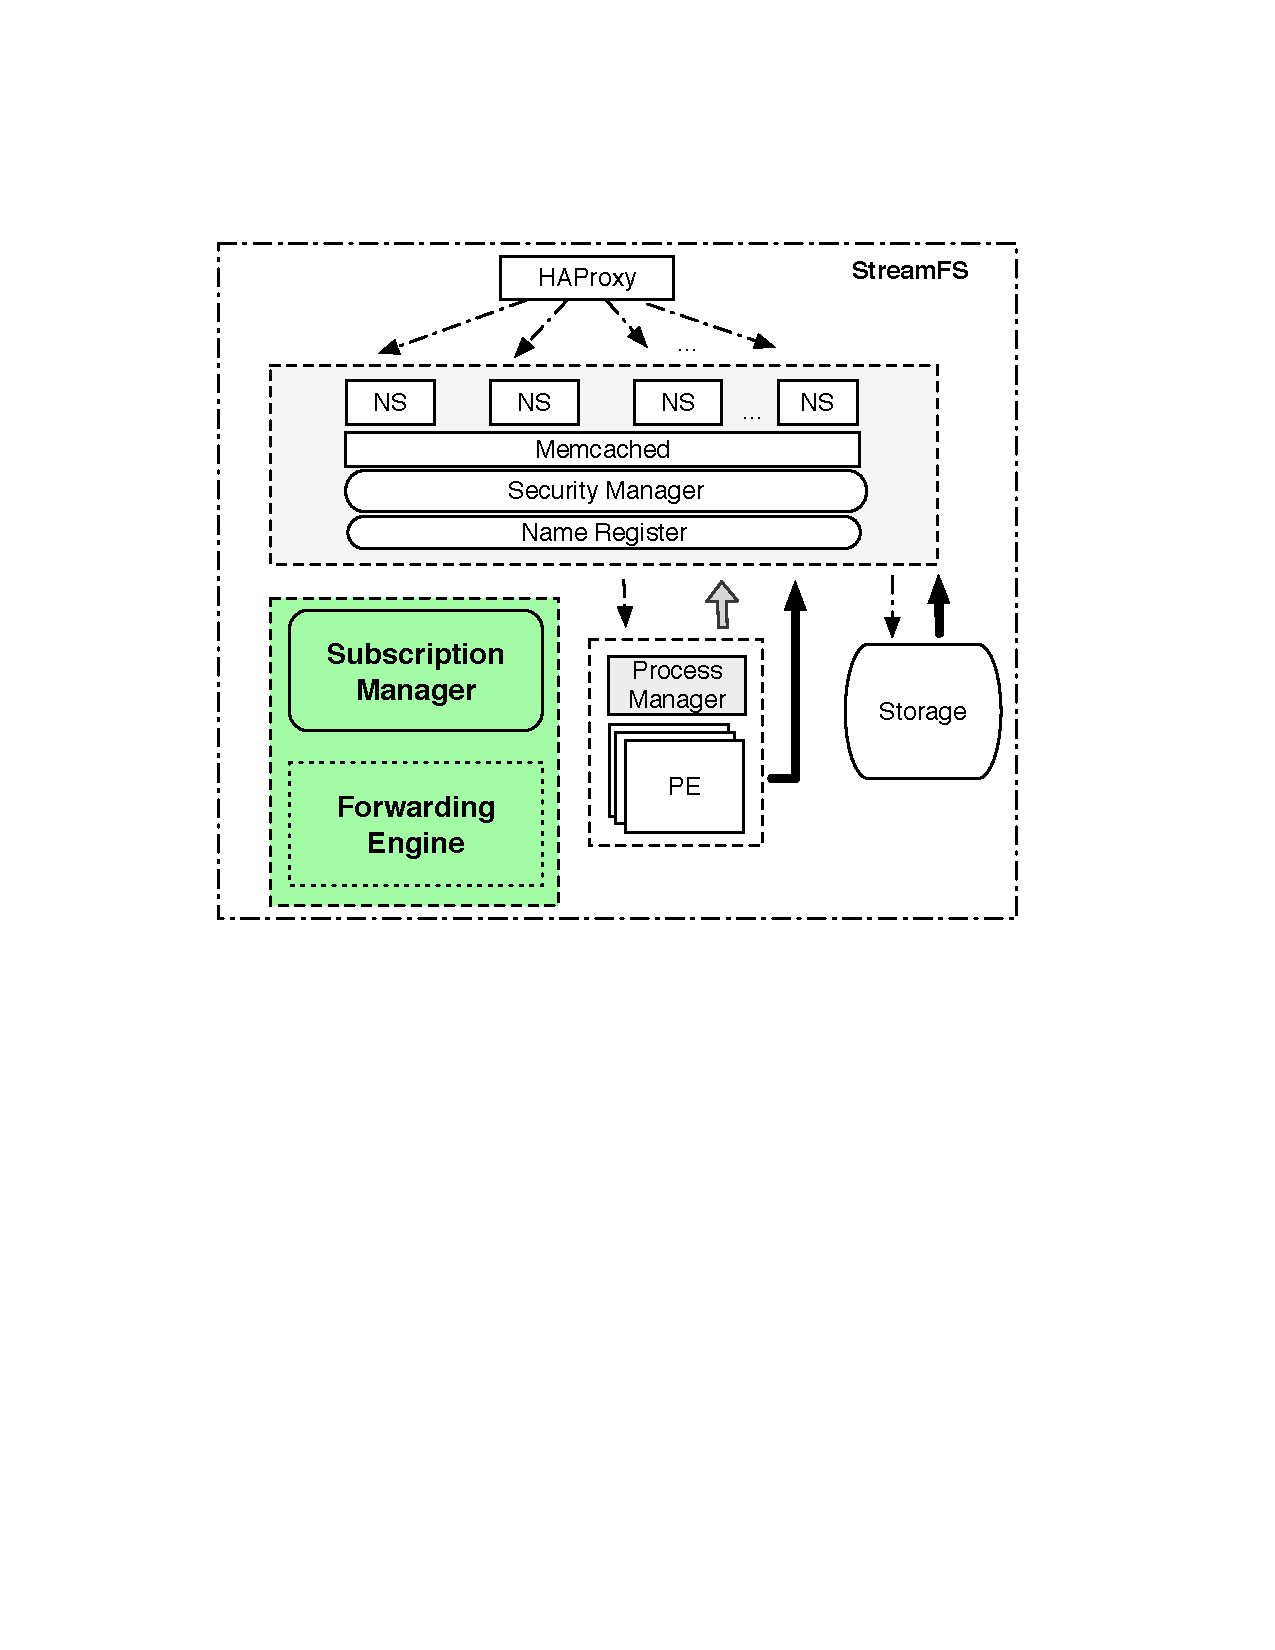
\includegraphics[width=.55\columnwidth]{figs/submngr}
\caption{}
\label{fig:submngr}
\end{figure}

The pub-sub system manager works with the name register to determine where to forward the incoming data.  When data arrives, it arrives
with a tag that contains the name of the publisher.  The subscription manager resolves the name to an object identifier and resolves
all the names for the object.  Then, it scans each of the names and matches them to a subscription.  If the subcription matches \emph{any}
name, the data unit is marked with the subscription id and sends to the forwarding engine.  The forwarding engine then
contact the forwarding sink and send it the data unit.  The subscription sink may be a processing element managed by the process manager.
If so, it is forwarded to the process manager's buffer and the process manager copies it to either an internal buffer for a
process that is running locally or sends it to an external process stub, which copies it in an internal buffer on the client side.
\section{Data Cleaning and Real-time Processing}

Data is coming in at different, independent rate from sensors and is produced asynchronously from internal processing elements.
For certain processes, processing the incoming data as quickly as possible is key, however, this is challenging for several reasons:
1) a process may subscribe to multiple, independent streams with asychronized report schedules and 2) interpolated values
should be avoided to minimize prediction inaccuracies in interpolated values.  Therefore, a process actually wants all the freshest
data from all the streams they are subscribing to, while minimizing the average time that the data for each respective stream has 
been waiting in the buffer.

Sensor data is fundamentally challenging to deal with because much of it must be cleaned before it can be processed.  For example,
it is not uncommon to receive readings that is out of operational range, that is erroneous with respect to the previous observed trend,
or to stop receiving readings altogether.  This implies the need for processing jobs to provide a level of filtering over the raw streams.
Once the data is cleaned, it is typically consumed more sophisticated processes that aggregate the information or use it for control
of the space or equipment.  We provide the mechanisms for handling both classes of processing jobs with our process management layer.
In the next section we will discuss our process management layer and how users can both submit jobs to StreamFS for management or link
their own external processing elements so that they can be managed through StreamFS but run outside of StreamFS.

We also discuss how we deal with the fundamental challenges that come with sensor data.  Specifically, we 
address \emph{re-sampling} and \emph{processing models}.  The incoming data does not have a common
time source, so combining the signals meaningfully involves interpolation.  There are various options that we
provide for performing the interpolation, chosen by the user depending on the units of the data.  For example,
temperature data may involve fitting a heat model with the data to attain missing values in time.  In addition,
aggregation is done as a function of the underlying constituents: they can be combined arbritarily, by adding
subtracting, multiplying or dividing corresponding values.  We provide an interface to the user that
allows them to specify how to combine the aggregate signals as a function of the child nodes in the entity-graph.
Futhermore, they can filter the data by unit.  This kind of flexibility useful for visualizing
energy consumption over time.



\section{Entity-relationship Model}

StreamFS supports symbolic links, which allows the user to specify non-hierarchical relationships.  Indeed, they can 
be used to express relationships which form a directed graph.  We find that many applications, such as control 
applications and applications that perform aggregation, precede their timeseries queries with multiple queries
to determine indirect relationships between streams.  Fundamentally, the queries were use to ascertain a multiple-hop
relationship between streams and could be easily and efficiently answered with a single graph query.
StreamFS maintains an entity-relationship graph (ERG) that uses the names and symbolic links to construct a queryable 
graph.

The ERG is used throughout our architecture; for answering graph queries by the user and for subscription topic-matching.
The latter is slightly different from the topic-matching mechanism traditionally available in pub-sub systems. 
We discuss the details of our approach in section~\ref{sec:ProcMngtSchedMain}.


\subsection{ERG to OLAP}
\label{sec:erg2olap}

Many of the operations that users perform are OLAP-style (online analytical processing) operations\cite{Gray1996}. 
OLAP databases build a logical hypercube along multiple dimensions.  The values in the cells are called 
measures.  Queries makes use of the cube to aggregate data along those dimensions.
We provide OLAP-style queries using the ERG.  This is similar to the work proposed by Chen et al.~\cite{Chen2008_olapgraph}.
The time dimension is fixed, the categorical dimension is determined by the hierarchy, and the unit are specified
by the user.

\begin{figure}[h!] %htbp
\centering
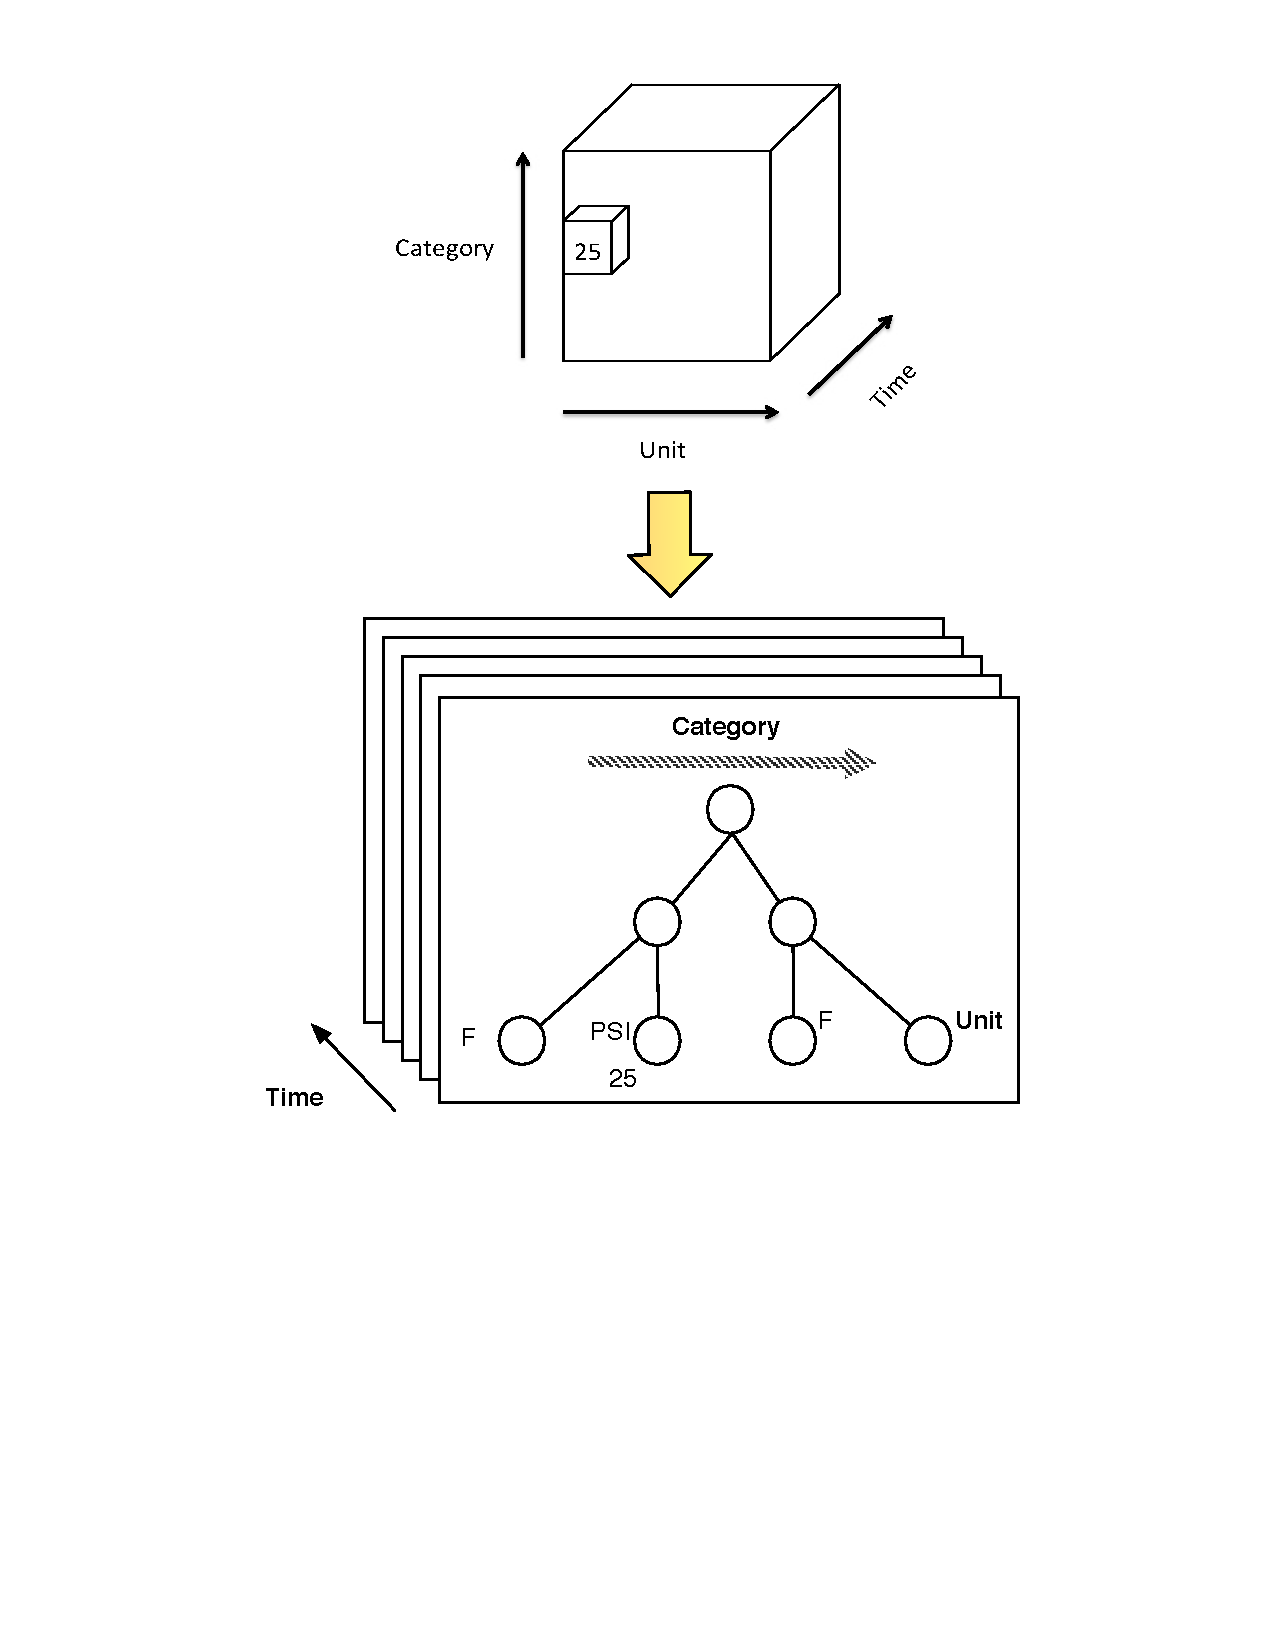
\includegraphics[width=.55\columnwidth]{figs/olaptoerg}
\caption{This figure shows how we translate the OLAP cube to a hierarchical ERG.  Note how the dimensions of the cube translate
to the graph.  The level of the subtree is the category, the unit is specified at the node, and there are values at each node
for every time slice.}
\label{fig:olap2erg}
\end{figure}

% where it can be used more effectively, and how to change the operation of the building -- through better equipment or activity scheduling -- 
% in order to optimize and reduce its energy consumption.
% For building-oriented energy analytics applications the building manager and occupants typically want answers
% to the following set of questions:
Below is a typical list of questions that can be answered efficiently with OLAP-style queries.  

\begin{enumerate}
\item How much energy is consumed in this room/floor/building?  On average?
\item What is the current power draw by this pump? cooling tower? heating sub-system?  Over
		the last month?
% \item How much power is this device currently drawing? Over the last hour?
%\item What percentage of the total building power is being drawn by the plug-load devices? 
% \item How much energy have I consumed today?  Versus yesterday?
\item How much energy does the computing equipment in this building consume?
%\item {\bf For all queries:} What's the trend over time?
\end{enumerate}
\vspace{0.08in}

% Notice, these question span space and time and require aggregation along a dimension, such as power.  
These questions require the ability to answer a series of questions
about energy flow -- energy data aggregated across multiple categories to determine how, where, and the amount used.  
The ability to \emph{slice and dice} the data allows the analyst to gain better insight into how the energy is being used.
Notice how questions translate into categorical and spatio-temporal queries.
There is also a hierarchical grouping characteristic to them.  For example, to answer the first question we must 
aggregate the data from the individual rooms up to the whole building (if the whole building data is not available)
% This hierarchical relationship
% is not as evident in the HVAC sub-components specified in the second question.  However,
% local hierarchically relationships do exist.  For example, 
Also, the cooling system consists of the set of pumps, cooling towers, and condensers in the HVAC system that push condenser
fluid and water to remove heat from spaces in the building.  We can model this as a set of objects and inter-relationships which inform how
to \emph{drill-down}, \emph{roll-up}, and \emph{slice and dice} the data -- traditional OLAP operations.
Figure~\ref{fig:olap2erg} shows how we translate an OLAP cube to a hierarchical arrangement of 
nodes in the ERG.  Time-range queries on any node translates to a slice in the cube along the time dimension.
\emph{Pivoting} along any dimension can be done by taking slices along the ``cube'' in the bottom of that
figure.
% The dynamic aggregation processing model accommodates many common situations where aggregation of feeds is the primary
% objective.  For example, consider a power meter attached to a fan running in a variable air-volume (VAV) unit.
% There can be several hundred VAV units throughout the entire building, one in each space that is controlled by 
% the HVAC system.  An energy auditor may want to determine the energy consumption with respect to either a space 
% or a system or by category.  If these three ``views'' are of interest, there would be three sub-trees in the namespace, 
% rooted at the building: \texttt{/hvac/}\dots\texttt{/vav/fan}, \texttt{/zones/}\dots\texttt{/vav/fan}, 
% and \texttt{/loads/}\dots\texttt{/fans}.  The first is the 
% sub-tree that represents the HVAC sub-components and their inter-connection, the second one describes the set 
% of zones, and the third one is a categorical partitioning of the loads in the building.  With dynamic aggregation,
% as data is received from the each fan stream, it continues up-stream to the aggregation points.
% So, for the total power consumption of the hvac system, you query \texttt{/hvac} (which includes the fans),
% for the total energy consumed in a particular space you query \texttt{/zone/4F/410} for example (which include the fan
% feeding that specific zone), and for a categorical aggregate, you could simple query 
% \texttt{/loads/}\dots\texttt{/fans}.

Unlike a typical OLAP cube, our ``cube'' is dynamic.  As new data comes in, it is immediately used.  Its arrival triggers
the aggregator to interpolate values for all other related streams at that point in time, aggregate them, and update all
the measures in the cube.  We find that many applications that require analytics, typically require OLAP style queries.
% For example, consider the problem of tracking the operational energy consumption of a building.  
We describe how this functionality is useful in performing energy audits and describe its use in
a mobile energy auditing applications presented in Section~\ref{sec:mobileaudit}.



% The main difference between this setup and traditional OLAP is the underlying dynamics of the
% inter-relationships: objects, particularly those meant to represent physical entities, are added and removed and 
% their inter-relationships change over time.  \emph{The natural evolution of buildings and activities 
% within them makes tracking energy-flow fundamentally challenging}.

The entity-relationship model helps simplify these problems, both as an interface to the user and a data structure for the aggregation processes.  
We argue that using the ERG in the building context is reduces the cognitive load and makes the formulation
of such queries easier.  The inter-relationships are explicitly specified and this allows users to 
maintain a structure that is more natural.  Also, it has been shown that a relational model loses this 
information~\cite{SenkoDB}.


% We argue that the 
% use of this model is a cleaner
% fit for this application scenario because it captures important semantic information about the real-world;
% facts critical for picking which questions to ask and how to answer them.  In contrast, it has been shown 
% that a relational model loses this information~\cite{SenkoDB}.

% Lets examine the requirements for answering the first question.
% A building is unware that there are rooms. Typically spaces in a building are called \emph{zones} and, 
% at construction time, walls are added to make rooms within zones.  This makes rooms an abstract
% entity, used to group associated items with respect to it.  It also means
% %The basic control unit for the Heating, Ventilation, and Air conditioning (HVAC) system as well as the electrical 
% %panels and plugs, is a zone, not a room.  
% we typically do not have a single meter that is measuring the energy of a room; it
% must be calculated from the set of energy-consuming constituents.

% What are the energy consuming constituents of a typical room?  It is the set of energy-consumers that
% are active within or onto the room.  Broadly, it consists of three things:

% \begin{itemize}
% \item Plug-loads
% \item Lights
% \item HVAC
% \end{itemize}
% \vspace{0.08in}

% For simplicity of demonstration, lets consider only plug-loads.  In our construction of an entity-relationship
% graph lets assume there are nodes for each plug-load item and each room.  For the room in question, the relationship
% between the plug-loads and the room is child to parent, respectively.  The total energy consumed by
% the plug-loads can be aggregated at the parent node, the room, so the user can query the room for
% the total.  Over time, plug-loads are removed and added to/from the room, but the relationship does not
% change.  This simplifies the query; to obtain the total consumption over time, the query need only
% go to the room node.  The parent-child relationship informs which constituents to aggregate over time
% to calculate the total.

% To realize this design we need to maintain the entity-relationship graph, present it to the user in a meaningful
% way; allowing them to update it directly to capture physical state and relationship changes.  We also need to
% use this graphical structure to direct data flow throughout the underlying network.  This allows us
% to accurately maintain the running aggregates as the deployment and activities churn.

% We present the graph to the user through a filesystem-like naming and linking mechanisms.  The combination of a
% hierarchical naming scheme and support for symbolic links allows the user to access and manipulate underlying objects
% and relationships.  Moreover, the underlying graph structure is overloaded with upstream communication mechanisms
% and buffering to allow data to flow from the data-producing leave nodes to the aggregation-performing
% parent nodes.  Furthermore, the buffering lets us deal with the streaming nature of data flow from the physical
% world to StreamFS and lets us maintain a real-time view of energy flow in the system.
% Traversing the graph provides a natural way for the user to implicitly execute the OLAP operations necessary 
% to give the user the kind of insight into energy usage in the building necessary to understand, optimize and 
% reduce it.

\subsection{Implementation Details}
The graph is maintained in memory.  A typical deployment contains about 10k nodes, so the memory footprint is not that large. 
In our deployments we kept the unit on its own machine with 4 GB of memory.  The footprint is typically several hundred to
about 1 GB in size.  We used a JUNG graph library~\cite{jung} to maintain the graph.

To achieve horizontal scalability, we propose that each ERG unit should be separated into distinct nodes in
a cluster and graph queries should be answered across the cluster.  This is a topic for future work, however, since a typical
building deployment does not require that level of scale.  A collection of buildings, managed through
a single instance of StreamFS, would likely require a clustered implementation of the ERG.



















\section{Related work}

%\begin{itemize}
% \item dashboard
% \item andrew's lightin control work
% \item Kamin's hvac control work
% \item BEMs
% \item sMAP stuff
%\item Buildsys 2010 work~\cite{hbci}
%\item distributed consistency management: COPS
%\item mobility: tracking things with RFID~\cite{rfid_gonz2006}
%\item mobility: tracking of people, wifi indoor localization
%\item entity-relationship graphs
%\item homeOS [microsoft]
%\item HP Cooltown~\cite{cooltown}
%\end{itemize}
Our work touches on several areas from smart home research to logistics.  In the building space, there has been
some interest in building various kinds of energy-related visual and control applications.
This work focuses on the object definition, tracking, and management component of the architecture proposed by 
Hsu et al.~\cite{hbci}.  Their work stratefied the set of challenges that one could potentially face if the application 
were deployed at scale.  Our
work, in constrast, bases its design rationale on a \emph{real deployment} that is taking place at scale in a building 
on our campus.  We focus on solving fundamental systems challenges in dealing with intermittent connectivity
and conflict resolution in tracking people and things over time.  We also focus on leveraging gestures to minimize
the cost of interaction for users, while maximizing the information we can attain about the state of the world.

% Tracking people/indoor localization
An important aspect of the Energy Lens is determining when people and things have moved.  This requires some form 
of indoor localization.  There's a large body of literature in the area of indoor localization with mobile phones ranging from 
using wifi~\cite{radar}, to sonar~\cite{cricket}, to ambient noise~\cite{abs}, and a combination of sensors on the 
phone~\cite{surroundsense, darwinphone}.  Dita~\cite{dita} uses acoustic localization of mobile phones and also uses the infrastructure 
to determine gestures in free-space that are classified into pre-defined control actions.  Each of these require relatively complex 
software and/or infrastrure.  
We take a radically different, simple approach.  We use cheap, easy to re/produce tags (QR codes), place them on things in the 
environment over incrementally and use the natural \emph{swiping gesture} that users make, when interacting with the Energy Lens 
application, to track when they have moved or when the objects around them have moved.  The working principal is to attain as much 
information from their gesture to determine when something/one has moved.  We discuss our heuristics in section~\ref{sec:swipes}.

% context-aware apps
ACE~\cite{ACE} uses various sensors on the phone to infer a user's context.  The context domain consists of a set of user activities
and semantic locations.  For example, if ACE can distinguish between {\tt Running, Driving, AtHome, or InOffice}.  ACE also infers 
the one from the others, so if the user is {\tt AtHome} then they are not {\tt InOffice}.  Energy Lens uses inference to determine
when a person or thing has moved.  Certain swipe combinations give us information about whether they moved and where they moved to or
whether an item moved and where it moved to.  The main difference is that we only infer context when a user is actively swiping, rather
than a continuous approach.  Pretching is a fundamental technique used in many domains.  However, the cost of a prefetch for mobile
application outways the benefits if the prefetched data is not useful.  Informed mobile pretching~\cite{IMP} uses cost-benefit analysis 
to determine when to prefetch content for the user.  In the Energy Lens context, we prefetch data based on their location swipes.
We also rely on pretching to anticipate loss of connectivity, not just to improve preformance.

% Tracking things
Logistic systems focus on the tracking of objects as the move through distribution sites to warehouses, stores, shelves,
and purchase.  Items are tracked through bar code or RFID readers.  However, the workload is very structured and well
defined.  The authors of~\cite{rfid_gonz2006} describe this structure and leverage it to minimize storage
requirements and optimize query-processing performance.  Energy Lens uses the QR codes as the tag and the phone as an active
reader.  As objects move, users scan those items to their new location.  However, objects may belong to one or
many people, they can be metered by multiple meters a day, and their history in the system
is on-going.  In contrast, a typical logistics workload has a start (distribution site) and end point (leaving the store
after a sale).  In our workload, relationship semantics are important; we need to know whether the meter is \emph{bound-to}
rather than simple \emph{attached-to} an item.  We discuss the difference later in the paper.
% In addition to traditional logistics-style queries -- \emph{What is the average time that it took coffee-makers to move from the 
% warehouse to the shelf and finally to the checkout counter in January of 2004?} -- energy-analytics requires queries to group
% partial traces from meter data by tracking what meters the item attached to over the specified time-frame.
% The Energy Lens system collects and manages this kind of information to enable such queries.
Furthermore, we take advatange of natural gestures the user makes with the phone while scanning QR codes to extract
information about the current location of the user or things.

% Tagging items, virtual services
The key idea in the HP Cooltown~\cite{bridgingphysical,cooltown} work is to web-enable `things' in the world, grouped-by
`place', and accessed by `people' via a standardized acquisition protocol (HTTP) and format (HTML, XML).  
Cooltown creates a web presence for things in the world either directly (embedded web server) or indirectly 
(URL-lookup tag) as a web page page that display the services it provides.  Many of the core concepts in Cooltown 
also show up in Energy Lens.  The main overlap is the use of tags in the world that contain a reference to a virtual 
resource, accessible via HTTP through
a network connection.  Cooltown, however, explicitly chooses not maintain a centralized relationship
graph, it leverages the decentralized, linking structure of the web to group associated web pages together.
Furthermore, things are assumed to not move.  People are the main mobile entities.  The kind of applications
we wish to support must track where things are and their specific inter-relationships.  We imposed a richer set of 
semantics on our, centrally maintained, relationship graph and use it to provide detailed energy information.


\section{Summary}

% StreamFS consists of over 20,000 lines of code and was implemented in mostly Java.  It was deployed across multiple
% buildings and several applications were built on top of it over a 2 years period.

In this chapter we gave an overview of the main components in StreamFS.  Each of the components addresses the concerns stated in 
section~\ref{sec:shortcomings}.  The filesystem name server expose a uniform namespace for access sensors and actuators in 
deployed throughout the building.  The timeseries database serve to store data streaming physical information and 
is optimized for the scan-style queries posed by applications.  These address points \ref{nw} and \ref{ts}.
We also include a pub-sub system which serves multiple purposes.  It provides real-time data forwarding for external
applications and forwards data internally to processing units that are specified or linked by the user.
This addresses points \ref{rt}.  Finally, we introduce processing elements, both internal and external to address
point \ref{proc}.  We also introduce an entity-relationship graph to deal with indirect relationships that are
expressed in the construction of names in the system.

In the next chapter we talk more about processing and discuss the details in the scheduler that help enable applications
that have certain delivery requirement.



\chapter{Process Management and Scheduling}

Data is coming in at different, independent rate from sensors and is produced asynchronously from internal processing elements.
For certain processes, processing the incoming data as quickly as possible is key, however, this is challenging for several reasons:
1) a process may subscribe to multiple, independent streams with asychronized report schedules and 2) interpolated values
should be avoided to minimize prediction inaccuracies in interpolated values.  Therefore, a process actually wants all the freshest
data from all the streams they are subscribing to, while minimizing the average time that the data for each respective stream has 
been waiting in the buffer.

Sensor data is fundamentally challenging to deal with because much of it must be cleaned before it can be processed.  For example,
it is not uncommon to receive readings that is out of operational range, that is erroneous with respect to the previous observed trend,
or to stop receiving readings altogether.  This implies the need for processing jobs to provide a level of filtering over the raw streams.
Once the data is cleaned, it is typically consumed more sophisticated processes that aggregate the information or use it for control
of the space or equipment.  We provide the mechanisms for handling both classes of processing jobs with our process management layer.
In the next section we will discuss our process management layer and how users can both submit jobs to StreamFS for management or link
their own external processing elements so that they can be managed through StreamFS but run outside of StreamFS.

% \input{ProcessMngt}
\section{Internal Processes}
Internal processes are jobs submitted to StreamFS that are written in Javascript and managed within a StreamFS cluster.

StreamFS distinguishes between nodes that represent streaming data sources in the real-world
and those that do not.  Those that do not, however, can be tagged as aggregation points.  As part of the 
tagging processes, a user specifies the units of aggregation, with additional options for cleaning
and processing.  Our contributions are:  

\begin{itemize}
\item Use of the entity-relationship graph to provide OLAP \emph{roll-up}, \emph{drill-down},
		and \emph{slice and dice} operations.
\item Show how sliding-window operations can be used on real-time data in combination with the entity-relationship
		graph to maintain accurate aggregates as the underlying objects and inter-relationships change.
\end{itemize}


% \subsection{Mapping OLAP to ERG}
\subsection{OLAP-style Aggregation}

% \begin{itemize}
% \item Introduction to OLAP.
% \item Explanation of ERG in StreamFS.
% \end{itemize}
Online analytical processing (OLAP) is a processing layer that provides summurization of data
from a set of underlying data repository (date warehouses).  Traditionally, OLAP is used to process
business data.  Business data summurization allows an analyst ask targetted questions about aggregates 
and trends in their data.  The data is typically multidimensional in nature and operations can be performed with
respect to those dimensions and their inter-relationship.

\subsubsection{Measures, Dimenions, and Levels}
Measures are the value, dimensions are the units of measure as well as time, and levels/hierarchy are 
explicit in the naming structure.

\subsubsection{Operations: drill-down and roll-up}
Drill-down and roll-up are made explicit in the structure.  You can drill down to individual readings or roll them
up into an aggregation point at a particular level in the hierarchy.

\subsubsection{Operations: slice and dice}
Slice and dice operations 

\subsubsection{Operations: pivoting}
\subsection{Dynamic Aggregation}
\label{sec:dynagg}
Dynamic aggregation combines the underlying entity-relationship graph with in-network aggregation.  It treats
each node in the graph as a potential point of aggregation on a particular data type.  For example,
if we need to compute aggregates of \emph{KW} data and we declare the node for a particular room as
the point of aggregation, we accept data from all children of that node that, whose units are in \emph{KW},
and add the streams together over pre-defined window size or pre-defined timeouts.

The scheme is hiearchical, so a node only accepts data from its children and only sends data to its parent.
StreamFS checks for cycles when before node insertion and prevents double-counting errors by only allowing 
aggregation-points that are roots of a tree that is a sub-graph of the entity-relationship graph.  In our deployment,
each view is a managed as an independent hierarchy.  So the hierarchy of \emph{spaces} is separate from
the \emph{inventory} hierarchy or the \emph{taxonomy} hierarchy.  This allows us to ask questions with a particular
view in mind, without conflict, and is a natural fit for our aggregation scheme.

% \subsubsection{How it works}
Although there are different semantics applied to different node types at the application layer, StreamFS only knows
about two types of nodes: (1) default nodes and (2) stream nodes.  The main difference is that \emph{default} nodes
are not explicitly associated with data coming from a sensor and \emph{stream} nodes are.  Furthermore, default
nodes can have children, while stream nodes cannot.  In our application, meters are represented by default nodes
and each stream of data they produce is a stream node.

When an aggregation point is chosen and enabled, dynamic aggregation places a buffer at the node for the type
of data that should be aggregated.  If we want to aggregate \emph{KW} data, we specify the type and send an enable-aggregation
request to the node through an HTTP {\texttt POST} to the path for that node.  The flow of data starts at the leaves when
a stream node received data from a sensor through HTTP {\texttt POST}.  As data arrives it is immediately
forwarded upstream to the parent(s).  If a node that receives data from its children is an aggregation point it buffers
the data, otherwise it fowards it to its parent.

Ignoring the timeouts for now, lets imagine the parent is a point of aggregation and its buffer is full.  At this point
the parent separates data into bins for each source and cleans it for aggregation through interpolation.  The main
operation is to \emph{stretch} and \emph{fill} that data with linearly interpolated values.  The \emph{stretch}
operation orders all the timestamps in increasing order and for each bin (signal) interpolates the values using the
first (last) pair of data points.  If there is only a single data point, the stretch uses it as the missing value.
The \emph{fill} operation find the nearest timestamps that are less-than and greater-than the missing sampling time, 
uses their values to determine the equation of a line between them and interpolates the missing value using that equation.
Once this is done for each signal, the values are added together for each unqiue timestamp and the aggregated
signal is reported to the parent, where the operation occurs recursively to the root.
Figure~\ref{fig:aggtree} shows an illustration of its operation.  

%problem:  the buffer size has to increase exponentially up the tree, in order to not drop any values.
%solution: chuck the data into default-buffer sized pieces and parallelize the interpolation using the interpolated tasks technique


%FILL IN WITH REAL GRAPH
\begin{figure}[htb!]
\begin{center}
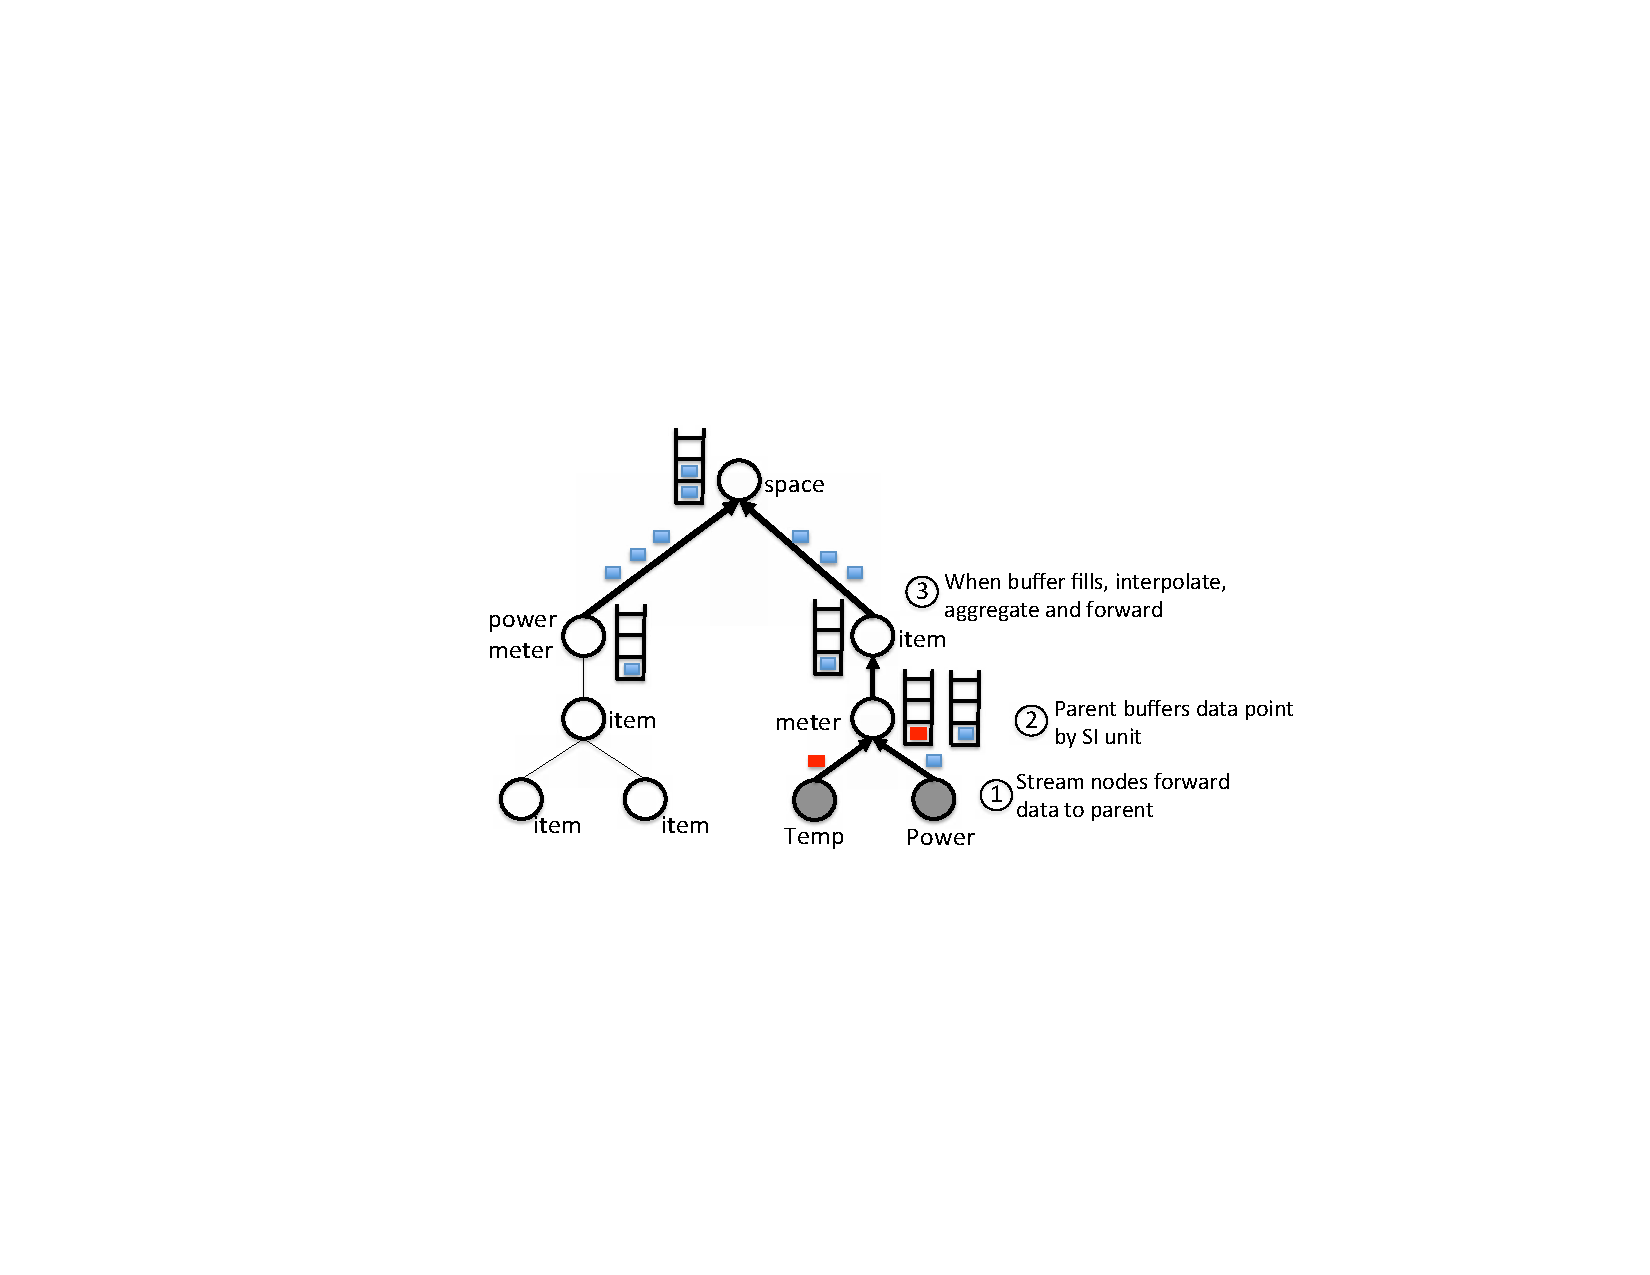
\includegraphics[scale=0.6]{figs/aggtree}
\caption{This shows an illustration of the aggregation tree used by \emph{dynamic aggregation}.  Data flows from 
the leaves to the root through user-specified aggregation points.  When the local buffer is full the streams
are separated by source, interpolated, and summed.  The aggregated signal is foward up the tree.}
\label{fig:aggtree}
\end{center}
\end{figure}

\subsubsection{Dealing with dynamics}
This approach deals with changes in the graph quite naturally.  All aggregation point deal only with local data, so
a node is only concerned about the children that give it data and the parent to send data to.  As objects in the environment
move from place to place and these changes are captured, the entity-relationship graph also changes to reflect the move.
This change in aggregation constituents is naturally accounted for in the aggregate.  If a child is removed,
it no longer forwards data to the old parent, therefore the aggregate will reflect that change.
Note, however, that changes in the entity-relationship graph are indistinguishable from energy-consuming items that have
been turned off.  For the purposes of aggregation, that is okay.

\subsubsection{Two scenarios}
We illustrate dynamic aggregation with a common usage scenario.  Imagine there are a number of people in a building,
each owning a number of plug-load applicances and a laptop.  Assume that when a person is in a room their laptop
is plugged in and when they leave the room they unplug their laptop and take it with them.  People come and go
throughout the day, changing the aggregate power consumption of the room and it happens.  In addition, some
of those people move to other rooms and plug their laptop in the new location.  As this happens, we will assume
all actions are being recorded in StreamFS.

%FILL IN WITH REAL GRAPH
\begin{figure}[htb!]
\begin{center}
\subfloat[Room 1 object and aggregate streams.]{%
            \label{fig:dynaggs1room1}
            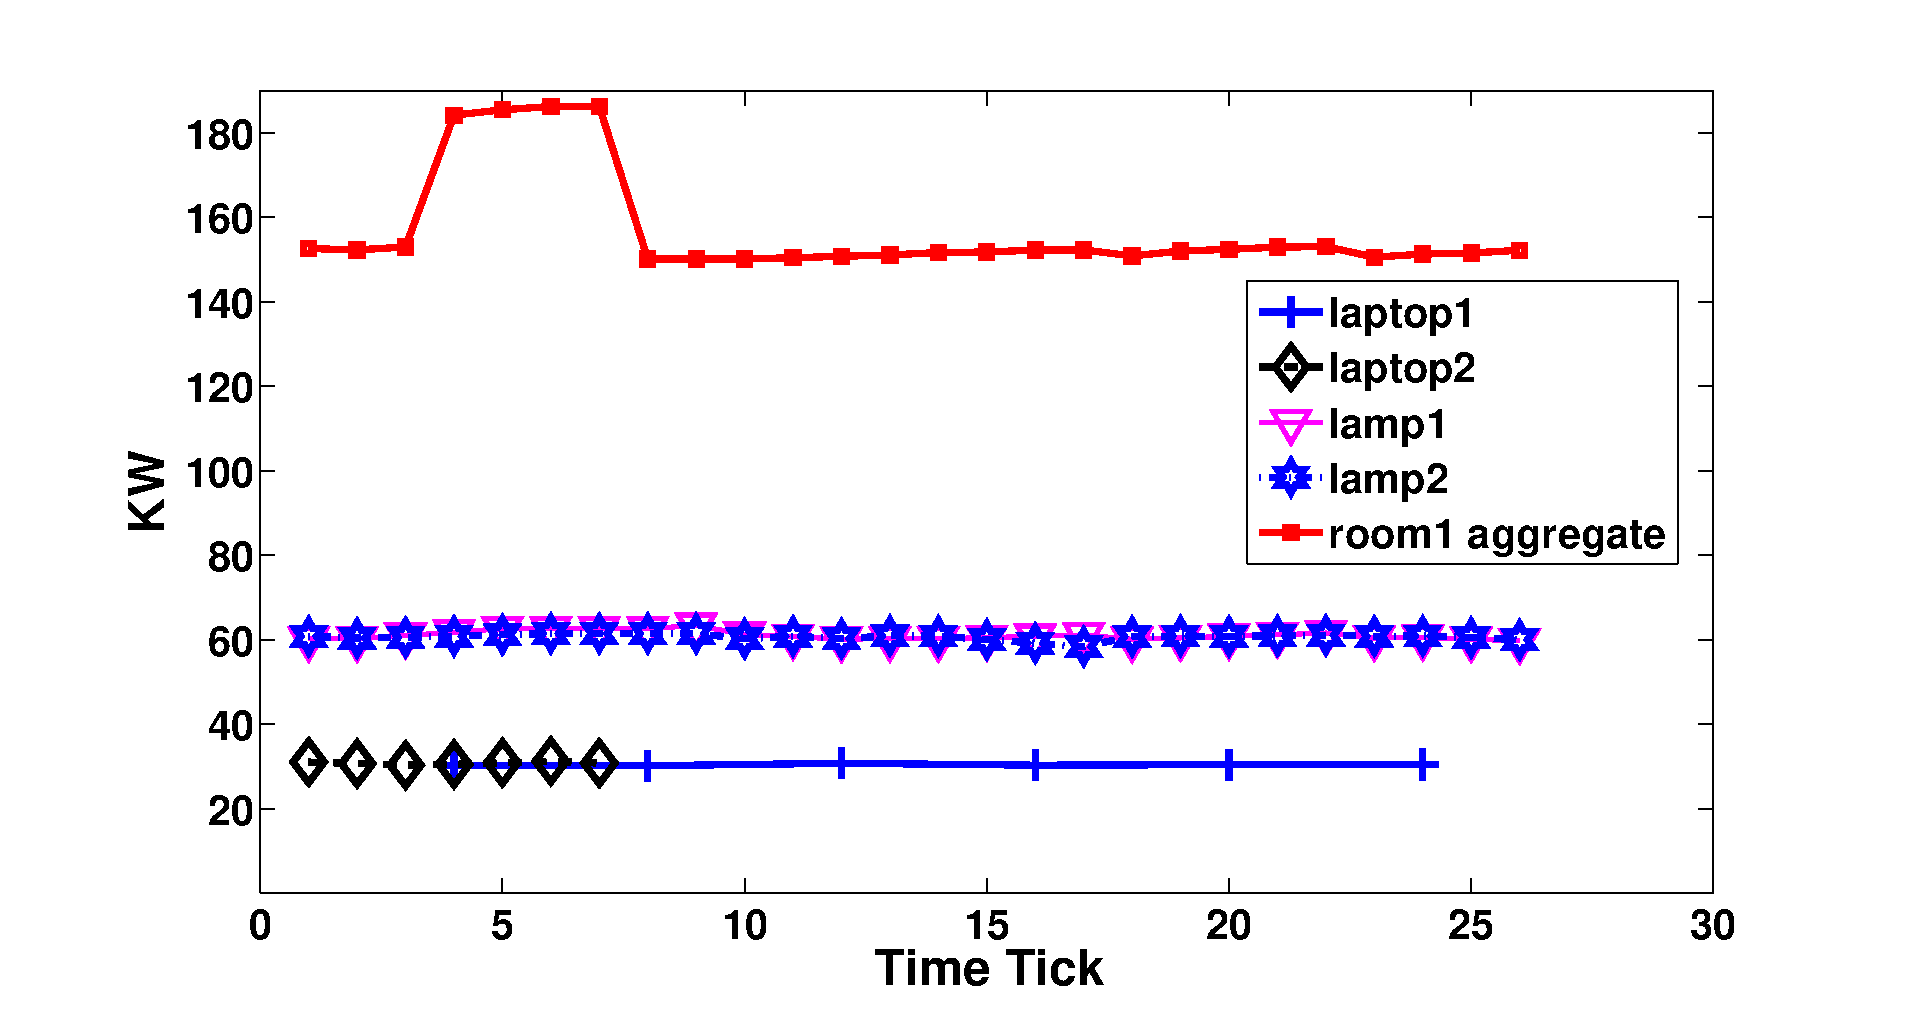
\includegraphics[scale=0.4]{figs/dynagg_scenario1_room1}
        }
\subfloat[Room 2 aggregate.]{%
            \label{fig:dynaggs1room2}
            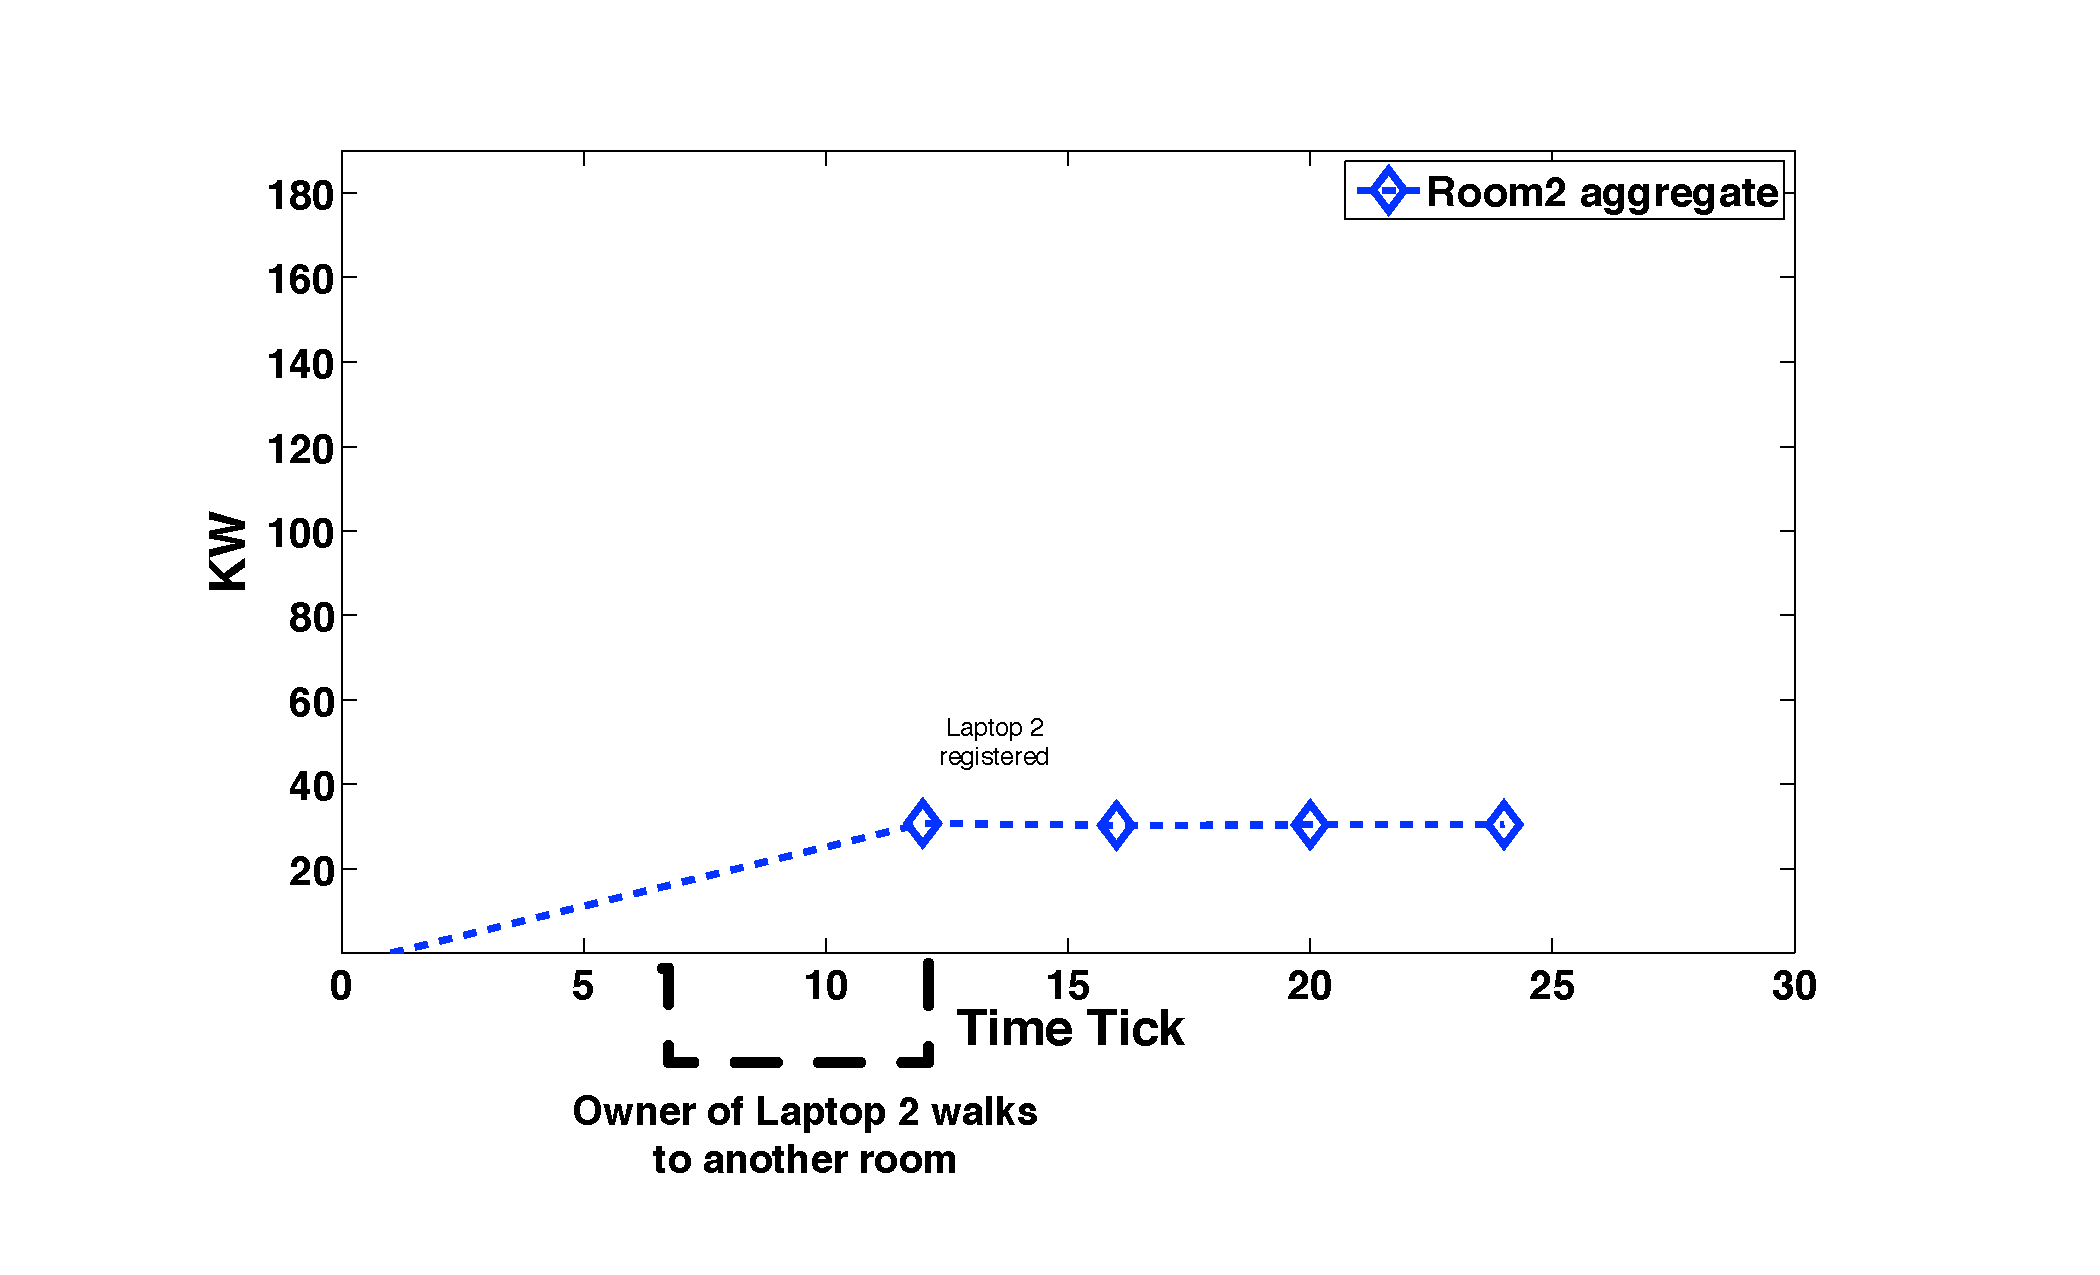
\includegraphics[scale=0.4]{figs/dynagg_scenario1_room2}
        }
\end{center}
\caption{
	The power consumes by a laptop in \emph{room 1} is shifted to \emph{room 2} a time t=7.  Notice the aggregagate drops in room 1
	while it rises in room 2.
     }%
\label{fig:multiroomagg}
\end{figure}

Figure~\ref{fig:multiroomagg} illustrate the aggregation results of that scenario.  Notice how...

% For demonstration lets have the user turn off on of their appliances when they leave as well.  This should cause that total
% room aggregate to drop, the person's personal aggregate to drop, but the other occupant's aggregate to remain
% the same.

% %FILL IN WITH REAL GRAPH
% \begin{figure}[htb!]
% \begin{center}
% 
\includegraphics[scale=0.39]{figs/blankbox}
% \caption{A room with items that belong to many users.  Person leaves with their item, aggregate falls.  Show aggregate.
% Person joins another room, aggregate in that room rises.  Show aggregate in the new room.  Compare before and after.}
% \label{fig:personaltotalagg}
% \end{center}
% \end{figure}

% Figure~\ref{fig:personaltotalagg} illustrate the results of the second sceanrio.  Note how...



\section{External Processes}

External processing jobs can be centrally managed in StreamFS as well.  In real deployments, it is often the case that
users do want to be limited by the particular libraries that are available to them in javascript or they have already made
a signficant investment in time writing and testing their own processing jobs.  We introduce an external client stub that 
re-directs data from standard in/out through a network connection to/from the StreamFS server.  The stub also interprets
process management commands to spawn and kill jobs and associate different subscriptions with different instances of a jobs 
running on the client side.

On startup, the client stub read a local configuration file that specifies the path to the job and metadata that describes
job.  These are used to register the job with StreamFS and set the metadata attributes.  The registration on the StreamFS 
server is exposed through an \emph{external process} file.  The user interact with an external job exactly the same way they
interact with an internal process job.  In order to spawn a job on the client, the user simply ``pipes'' a stream file 
to the external process file.  The creation of the pipe/subcription send a spawn message to the client and starts the associated
job on the client.  Once the process is started, data from the stream(s) is forwarded to the client, which writes it to the 
standard-in of the client job.  Starting a job also creates a stream file the StreamFS server.  Any data that's produced by the job
and written to standard-out is re-directed to the server and made available through the stream file.

This desgin is consistent with the semantics of pipe/subscription management and functionality.  Recall, internal processes
work the same way and this allow us to stay consistent with the file-centric principal whereby \emph{everything is managed
through the filesystem itself as a file}.



\section{Freshness Scheduling}
Process execution parameters are set by the user when a process element is created.  Generally, job scheduling is strictly driven
by these parameters.  However, in our deployments we found there were job pipe sinks that required a \emph{minimum freshness}
property for the set of data points in the buffer upon consumption.  In this section we discuss our scheduling algorithm in
relation to providing this property.% and present some experimental results.


\subsection{Maximizing Data Freshness}
\label{sec:freshness}

Data is coming in at different, independent rate from sensors and is produced asynchronously from internal processing elements.
For certain processes, the freshest
data from all the streams they are subscribing to is necessary; while minimizing the average time that the data for each respective 
stream has 
been waiting in the buffer.


\begin{algorithm}[h!]
 \SetAlgoLined
 Given a full buffer $b[n]$:\\
  \For{all elements in the $b$}{
  (1) Calculate the staleness of element $i$ and add to total staleness, $S_n$\;
  \For{all other elements in the buffer}{
    (1) Determine the next report time $D_i$ for this element\;
    (2) Determine the staleness of all the elements if we wait until $D_i$\;
    (3) If it is the smallest staleness figure calculate, replace minimum cost, $S_l$.
    }
  }
  \If{$S_l$ is less than $S_n$}{
  (1) Wait until later to consume\;
  \Else{
  (1) Consume now}
  }
 \caption{\texttt{min\_buffer} algorithm.}
 \label{alg:min_buffer}
\end{algorithm}


Some streams show lots of variability in its value distribution over time; driven by the underlying dynamics of the system being 
monitored.  For example, the power
consumption of an active server or laptop tends to have a varying power-draw profile over short time scales.  
For jobs doing aggregation of 
streaming data, it is often the case that the time when the last reading was received is very different across streams.  

\begin{figure}[t!] %htbp
\centering
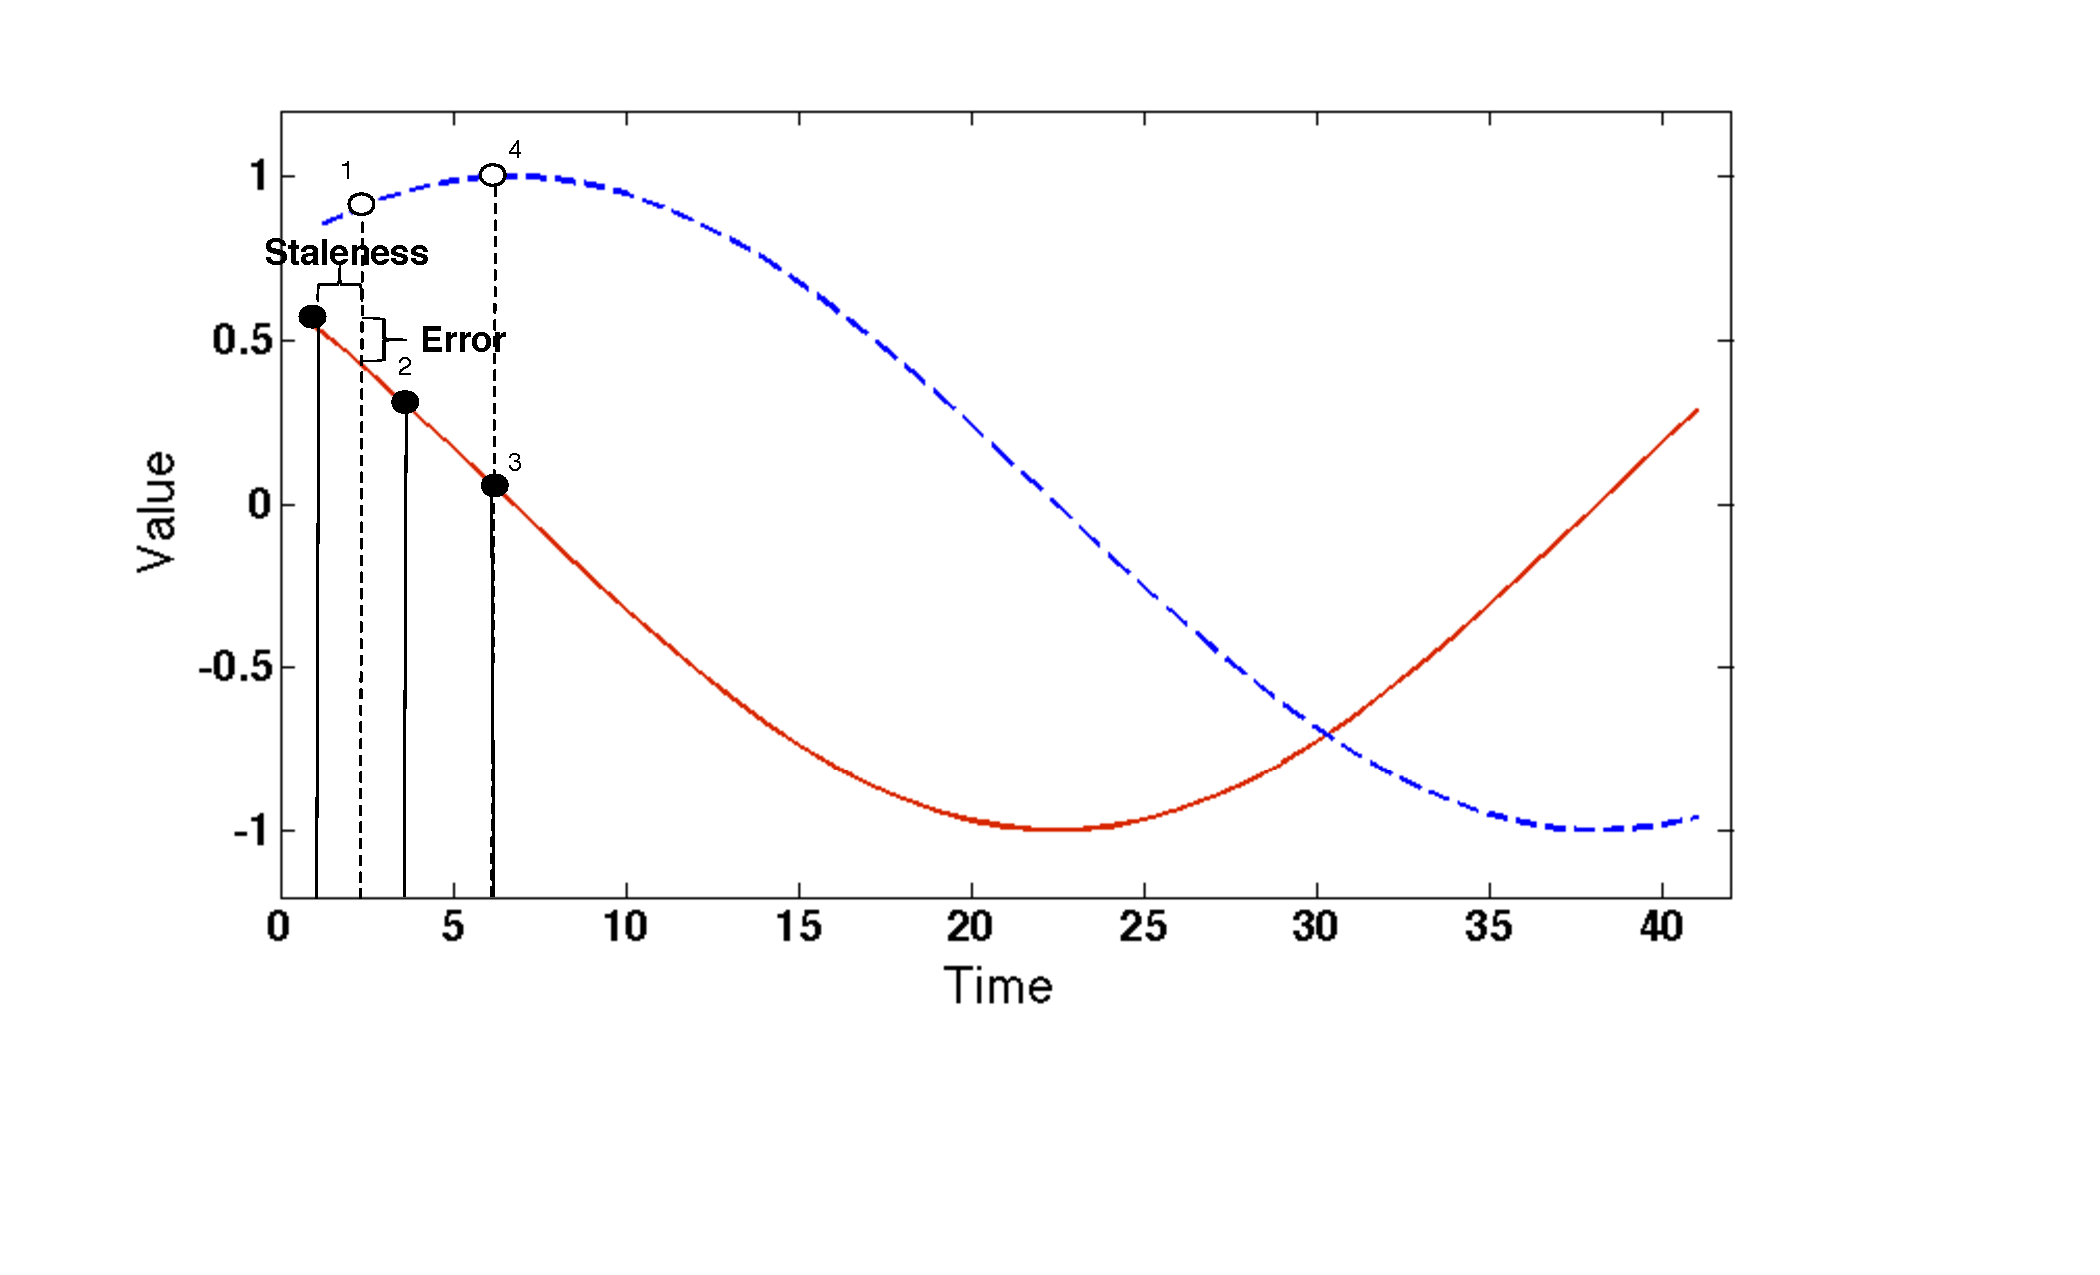
\includegraphics[width=0.75\columnwidth]{figs/sched_example.pdf}
\caption{This figure shows an example of two streams with different sampling frequencies.  Since we do not know the underlying fundamental frequency
of the phenomenon, our algorithm attempts to minimize error by minimizing staleness (or the average time a data point is in the receive buffer).}
\label{fig:sched_example}
\end{figure}

For example, consider two rapidly changing streams, as shown in Figure~\ref{fig:sched_example}.  
Each line represents the fundamental frequency of a different physical phenomenon.  The vertical lines represent reports times, as
observed at the StreamFS server; the time when the data points from those sensors are received.  
The circular dots show the value of the 
measurement that is in the buffer.  Assuming we have a subscriber that subscribes to only these two streams, the point labled with a 
`1' shows the first time that we can aggregate the two readings, `2' shows the second time, etc.
Note, the ideal aggregator \emph{minimizes} aggregation error in the sum, as specified in the figure.  Since a measurement was received 
at time t=2 and t=3, there will be some error associated with the sum -- the difference between the actual
value of the phenomenon at time t=3 and the value in the buffer (received at time t=2).  \emph{The longer we wait to compute the 
aggregate, the higher the error; until it resets when a new reading arrives}.

StreamFS does not know the underlying fundamental frequency of the phenomenon being measured, so it uses the staleness of the measurement to
approximate the error and a running report average for each stream to decide when it is best to compute the aggregate operation.  
Since the fundamental frequency is unknow, the driving assumption is that the more stale the reading, the higher the measurement error.  
Our measurement scheduler attempts to \emph{minimize aggregation error
by minimizing average buffer staleness} -- the time between the when the computation is taken and when the data point was received.  Note again
from the figure, that the best time to take a measurement is at t=6, since both data point come in at the same time and will have an average staleness
of 0.
% The ideal aggregation scenario is to
% combine the streams from the latest readings for both streams.  That way you minimizing the offset difference between during aggregation.
% If stream 1 produces a reading every three seconds and stream two produces a reading every two seconds, and you aggregate the readings every time you
% have at least one reading from both streams, every three seconds.  Sometimes the reading from the two-second stream will be one second old.
% If run the computation \emph{now}, the total staleness of the buffer is 1 second, if we wait on more second the total staleness is still one second, because
% at t=4 seconds, the three-second stream will be one second old.
For applications that wish to display the freshest aggregate (and approximate minimum error) we provide an algorithm
called \texttt{min\_buffer}.

The \texttt{min\_buffer} algorithm discards readings until two conditions are met:

\begin{enumerate}
\item There is at least one data point from each stream in the subscription buffer.
\item The staleness factor is minimized within the immediate time window.
\end{enumerate}

% This is of particular interest to controllers that need to make control decision based on the freshest data possible and can tolerate some variability
% in the completion time of the control task.  It is also useful in analytical jobs that want to process the latest data from multiple streams while also
% allowing some variability in the completion of the processing task.  
Note, there is a fundamental tradeoff
between the staleness factor and variability of consumption.  It is sometimes better to wait for the next incoming data point than it is to use what
is currently in the buffer, as waiting will decrease the overall staleness factor.  Other times, it is better to consume the buffered data immediately.
This causes a certain amount of variability in the delivery period to the control process.  However, for some applications, this is a reasonable tradeoff
to make.  Making use of the freshest data is desirable for minimizing errors, either in the control of a system or the calculation of some aggregate 
state.
Generally, the error grows with staleness, therefore the goal of this mechanism is to continuously minimize the error associated with staleness through
scheduling.


\begin{figure}[t!] %htbp
\centering
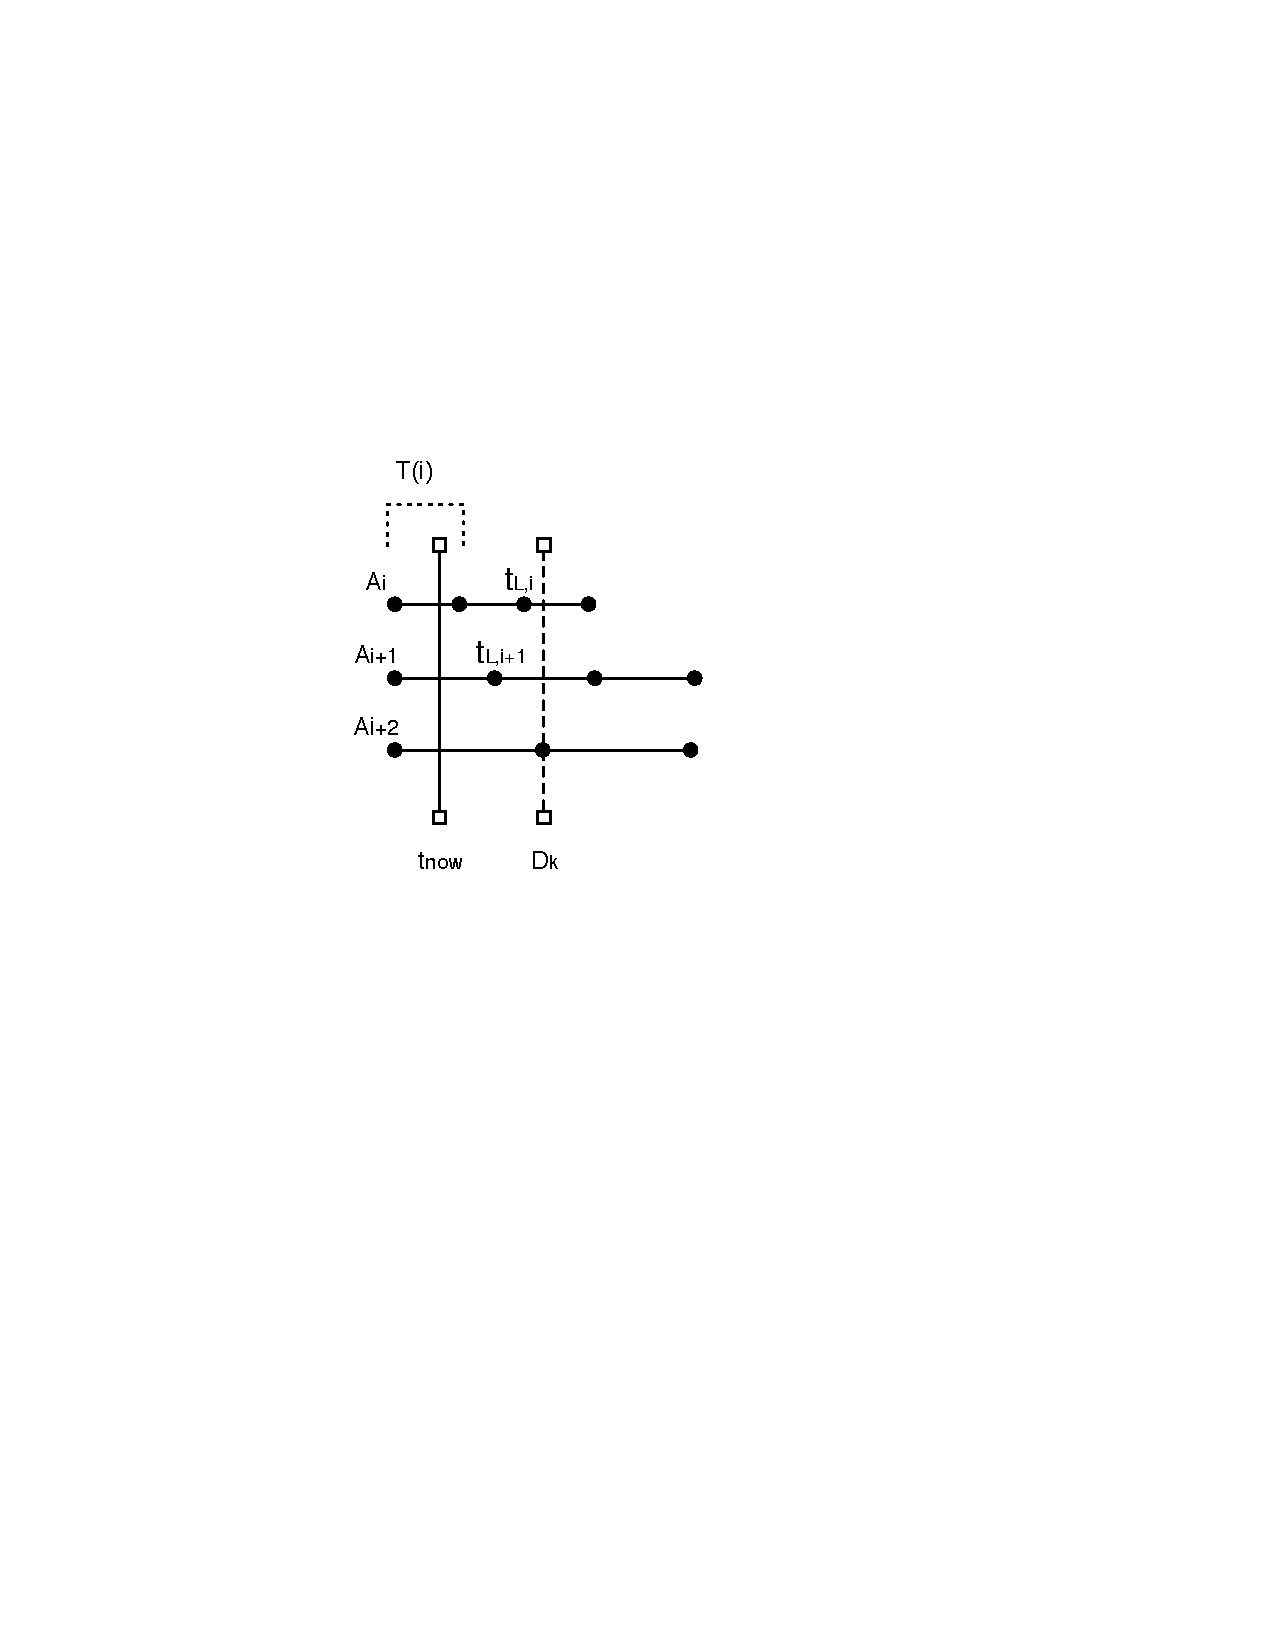
\includegraphics[width=0.75\columnwidth]{figs/min_buffer}
\caption{Multiple streams in a subscription and their associated parameters.}
\label{fig:min_buffer}
\end{figure}

Let $A_{i}$ be the arrival time of the last data point received from stream $i$ and $D_{i}$ be the arrival time for the next data point from stream $i$
and their relationship as described in Equation \ref{eqn:deadline}, where $T(i)$ is the average period between the arrivals from stream $i$.

\begin{equation}
D_{i} = A_{i} + T(i)
\label{eqn:deadline}
\end{equation}


Periodically, our algorithm runs and checks if there is a data point for each stream in the subscription.  If so, the \emph{min\_buffer} algorithm runs 
and effectively decides whether to execute the job on the current buffer immediately or whether to wait until later, when the \emph{staleness factor} of
the buffer will be at a minimum.  This decision is driven by Equation~\ref{eqn:later_better_condition}, whereby we find the next deadline, computed with
Equation~\ref{eqn:last_deadline}, for each stream in the set and determine the staleness factor will be for the entire buffer if we wait until that deadline arrives.

\begin{equation}
t_{L,i} = A_{i} + \Bigl\lfloor \frac{D_{k}-A_{i}}{T(i)} \Bigr\rfloor T(i)
\label{eqn:last_deadline}
\end{equation}

If there is no deadline $D_{k}$ for some stream $k$ such that Equation~\ref{eqn:later_better_condition} holds, then we execute now.  Otherwise we choose to wait
until $D_{k}$ for the stream whose next deadline minimizes the staleness factor of the buffer.


\begin{equation}
\sum_{i=1}^{k-1} D_{k} - t_{L,i} < \sum_{i=1}^{k} t_{now} - A_{i}
\label{eqn:later_better_condition}
\end{equation}

Algorithm~\ref{alg:min_buffer} shows the pseudocode for the \texttt{min\_buffer} algorithm.


\subsection{Results}

We test our hypothesis in this section by using EMD to remove low-frequency trends in the data
and run correlation calculation at overlapping IMF timescales.  We discover that EMD allows us
to find and compare high-frequency instrinsic behavior that is spatially correlated across
sensors.  We begin with a small set of three sensors (EHP, GHP, light) and expand our scope
to include all the sensors in the dataset.



\subsubsection{Initial analysis}
Lets consider the simple example of Section \ref{problem} where we would like to know if the EHP trace is correlated with the two other traces.
Recall that the correlation coefficients of the raw feeds was $0.7715$ and $0.6370$, corresponding to the light 
and GHP, respectively.
As stated in previous section this result is correct but not so meaningful, since most of the traces
display the same diurnal pattern.
Figure \ref{fig:emd} and Figure \ref{fig:emd2} show the EMD decomposition of the three traces.
For each trace, EMD has retrieved three IMFs that highlight the higher frequencies of the traces.

Figure~\ref{fig:emd} shows the normalized raw trace (top) and EMD output IMFs and residual as well as the 
correlation coefficients calculated on the IMFs for the EHP and
light traces.  The correlation coefficients are $0.43909$, $0.49344$ and $0.63469$ corresponding to the IMF1, 
IMF2, and IMF3, respectively.  Notice the high correlation between the high-frequency IMFs.
We know that the light and EHP serve the same room, and their high-frequency IMF correlation corroborates
our prior knowledge.
Figure~\ref{fig:emd2} shows a complementary result, for the EHP and GHP comparison.
The correlation coefficients for the EHP and GHP IMFs suggest that the two may be independent.  In fact, they
\emph{are} indepdent; they serve completely different rooms in the building!

EMD allows us to remove low-frequency trends that add noise to the original analysis.
By comparing IMFs, we see both intrisically correlated and \emph{uncorrelated} behavior.  In the next
section we expand our analysis and show the effectiveness of our methodology. 
% Although promising, these results must be validated across the rest of the
% dataset to confirm their significance.  


\subsubsection{Validation}
To validate the effectiveness of our approach, we analyze the same three-week time span for \emph{all} 674 
sensors deployed in the building.
For each trace $S$ we compute two scores: (1) the correlation coefficient between $S$ and the EHP trace
and (2) the average value of the IMF correlation coefficients.

\begin{figure}[tbh!]
\centering
 \subfloat[Raw traces correlation coefficients]{\label{fig:histo1}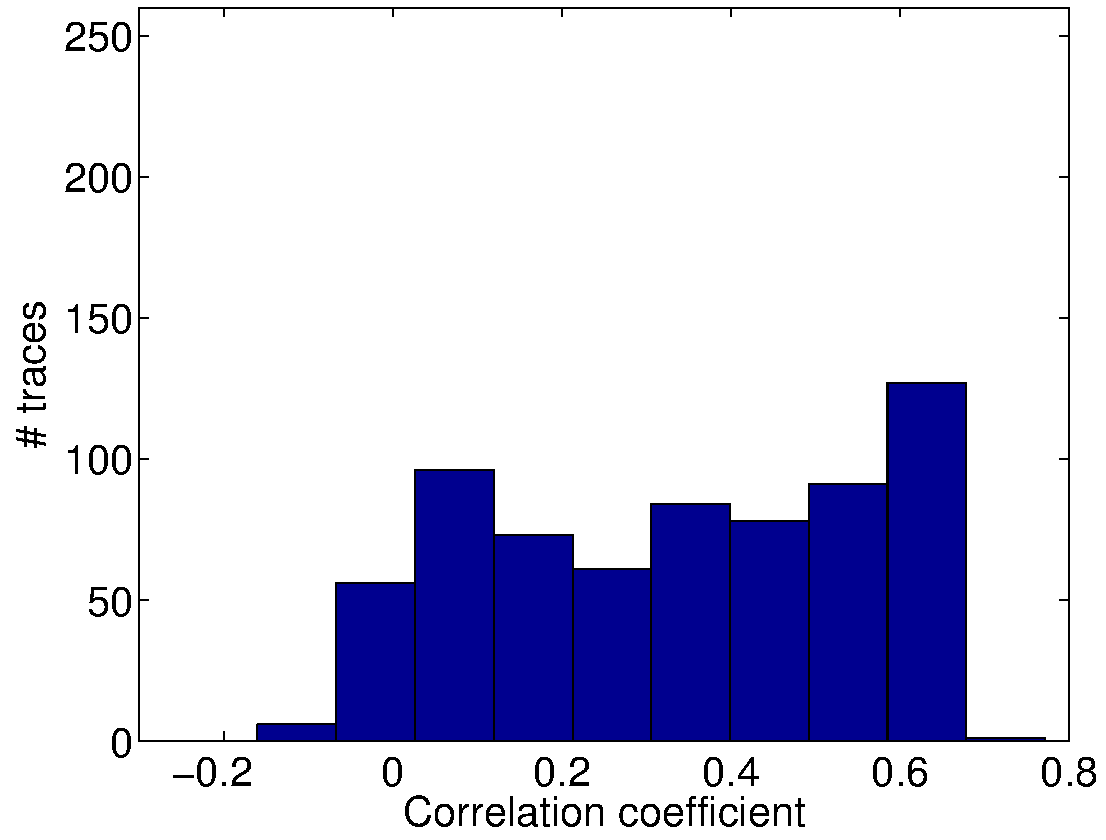
\includegraphics[width=.43\textwidth]{figs/allFloors_week1_week4_corr_abs-eps-converted-to}}
 \subfloat[Average IMFs correlation coefficients]{\label{fig:histo2}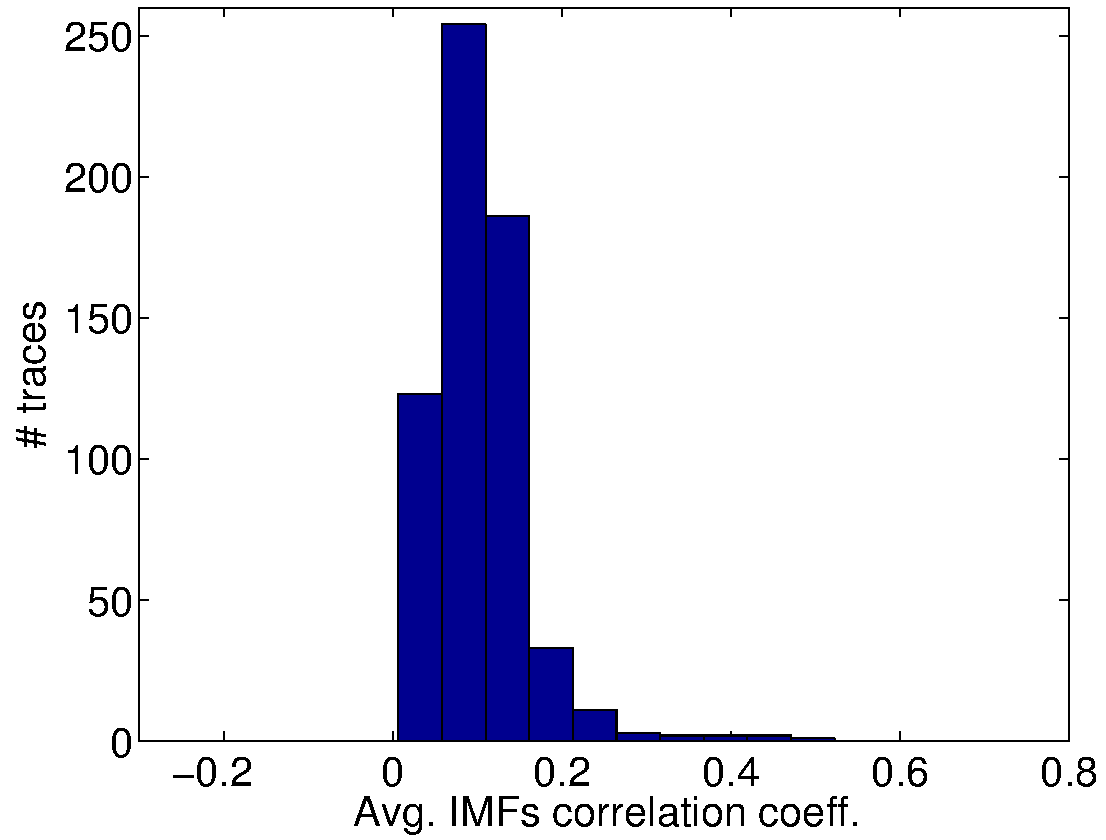
\includegraphics[width=.43\textwidth]{figs/allFloors_week1_week4_emd_abs-eps-converted-to}}
 \caption{Distribution of the correlation coefficients of the raw traces and correlation coefficients average of the corresponding IMFs using 3 weeks of data from 674 sensors.}
\label{fig:histo}
\end{figure}

\begin{figure}
\centering
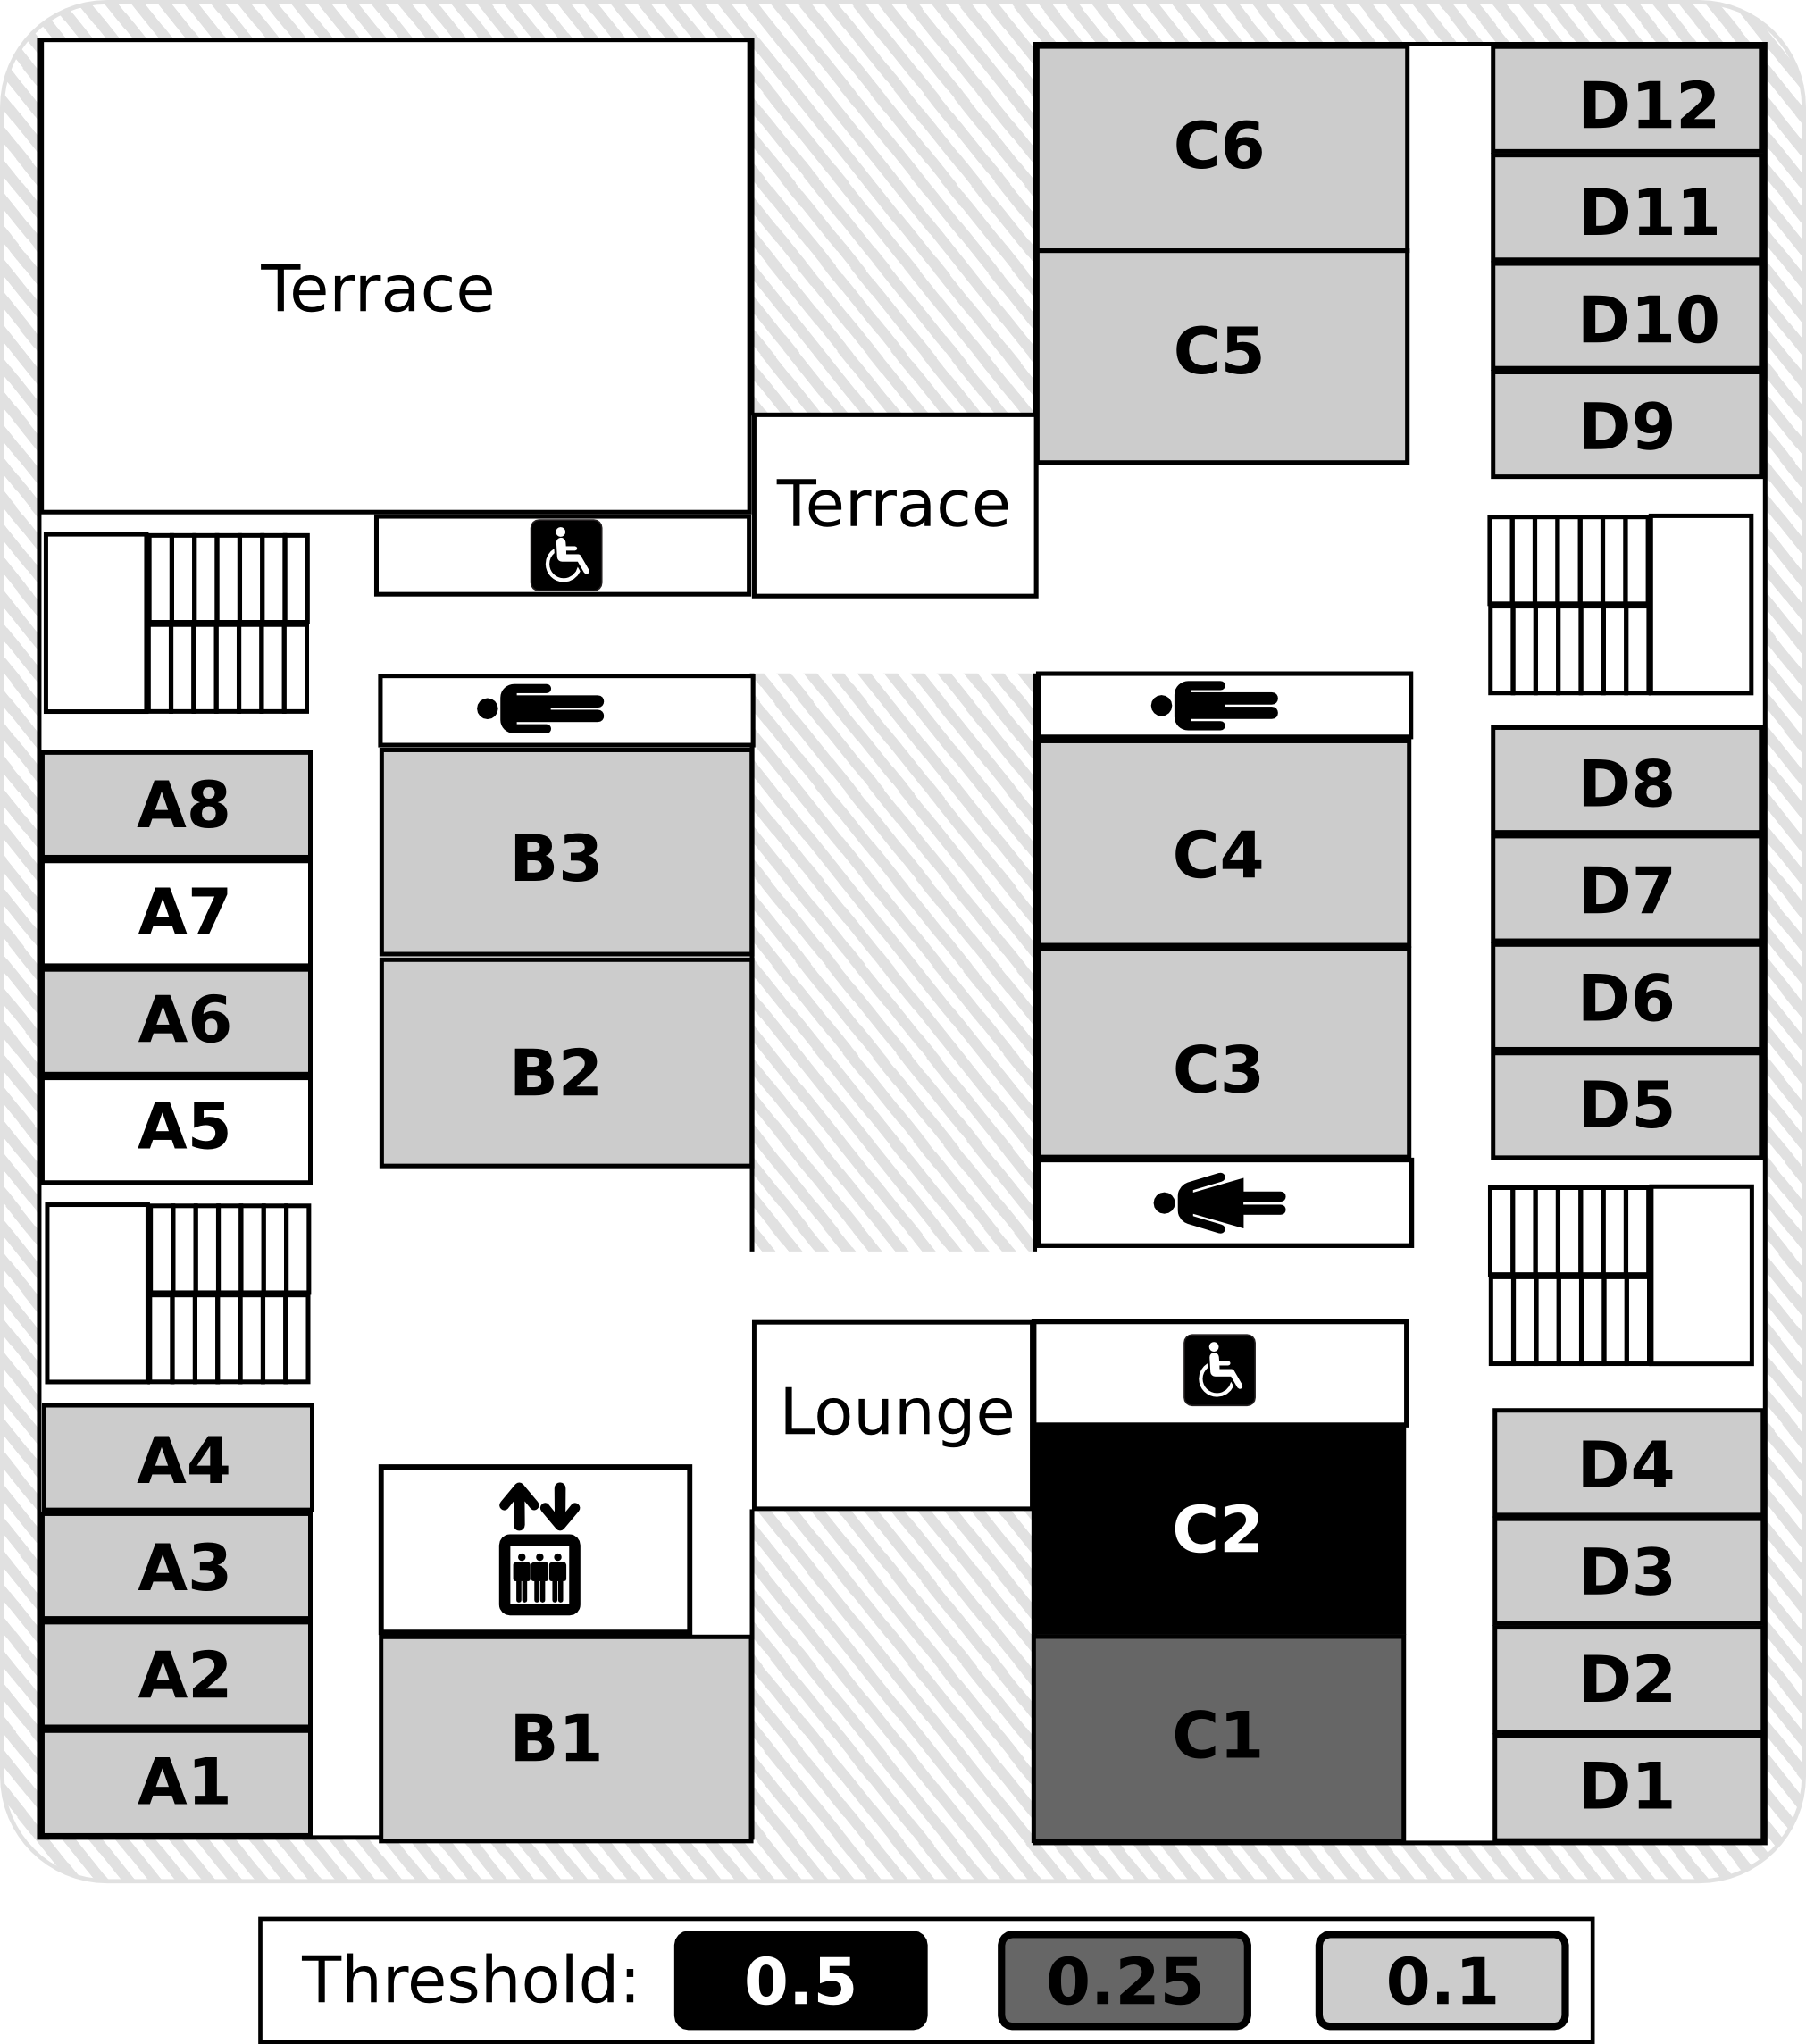
\includegraphics[width=.45\textwidth]{figs/floorMap.png}
\caption{Map of the floor where the analyzed EHP serves (room $C2$). The location of the sensors identified as related by the proposed approach are highlighted, showing a direct relationship between IMF correlation and spatial proximity.}
\label{fig:map}
\end{figure}

Figure \ref{fig:histo1} shows the distribution correlation coefficients.  Notice
that a large fraction of the dataset is correlated with the EHP trace.
\emph{Half} the traces have a correlation coefficient higher than $0.36$.  As expected, the underlying
trend is shared by a large number of device.
Although the highest score (i.e. $0.7715$) corresponds to the light in the same room that the EHP serves,
there are 118 pumps, serving all areas of the building, with a correlation higher than $0.6$.
Using only these results, it is not clear where the threshold should be set.  The distribution is close to 
uniform, making it difficult to 
know of how well your threshold discriminates against unrelated traces.
% Moreover, the distribution of the traces is almost uniform, thus, discriminating correlated traces is a laborious task.

Figure \ref{fig:histo2} shows the distribution of the average correlation value for the IMFs of
each trace and the EHP.  The number of traces correlated in the high frequency IMFs is significantly smaller
than the previous results. It's clear from the distribution that only a small set of devices are
\emph{intrinsically correlated} with the EHP.  In fact, \emph{only 10 traces out of 674} yielded a score higher than 
$0.25$. This allows us to easily rank traces by correlation.

Upon closer inspection of the 10 most correlated IMF traces, we find that there is a spatial relationship
between the EHP and the ten devices.  In fact, there is a direct relationship between score and distance from
the areas served by the EHP.  Figure~\ref{fig:map} shows a map of the floor that contains the rooms served by this
EHP.  The EHP directly serves room $C2$.  We introduce a correlation threshold to cluster correlated traces by score.
We highlight rooms by the threshold setting on the IMF correlation score.
When we set the threshold at $0.5$ we see that the sensors that have a correlation higher fall within room $C2$ --
the room served directly by the EHP.  As we relax the threshold, lowering it to $0.25$ and $0.1$ we see radial expansion from $C2$.  The trace with the highest score, $0.522$, is the trace corresponding to the lighting system \emph{in
the same room}.
The two highest scores for this floor (i.e. $0.316$ and $0.279$) are the light and EHP traces from next door, room $C1$.
Lower values correspond to sensors measuring activities in other rooms that have no specific relationship to the analyzed trace.  The results show a direct relationship between IMF correlation and spatial proximity and \emph{supports our initial
hypothesis}.


% Interestingly, the IMFs correlation coefficients reveal the spatial correlation of the sensors.
% Figure \ref{fig:map} is the map floor where the EHP trace is measured.
% Specifically, the EHP reports heating activity in the room $C2$.
% in the simple scenario the GHP is located in the room A5.



\section{Summary}

% StreamFS consists of over 20,000 lines of code and was implemented in mostly Java.  It was deployed across multiple
% buildings and several applications were built on top of it over a 2 years period.

In this chapter we gave an overview of the main components in StreamFS.  Each of the components addresses the concerns stated in 
section~\ref{sec:shortcomings}.  The filesystem name server expose a uniform namespace for access sensors and actuators in 
deployed throughout the building.  The timeseries database serve to store data streaming physical information and 
is optimized for the scan-style queries posed by applications.  These address points \ref{nw} and \ref{ts}.
We also include a pub-sub system which serves multiple purposes.  It provides real-time data forwarding for external
applications and forwards data internally to processing units that are specified or linked by the user.
This addresses points \ref{rt}.  Finally, we introduce processing elements, both internal and external to address
point \ref{proc}.  We also introduce an entity-relationship graph to deal with indirect relationships that are
expressed in the construction of names in the system.

In the next chapter we talk more about processing and discuss the details in the scheduler that help enable applications
that have certain delivery requirement.




\chapter{Filesystem Metaphore, Naming, and Verifiability}

From our experience with building applications, there are a clear set of requirements that are necessary.  Most applications
construct the notion of context using the naming convention ascribed to a sensor stream.  The name conflates the notion of system,
space, and type information.  At the very least, these three should be supported, however, often other categorical needs must be
met to perform various kinds of aggregate statistical, analytics, and control.  In addition, we need to support the management of
processing jobs that process stream data and provide integrated management facilities for them.

Building applications are essentially monitoring and control applications built on the streams generated by sensors embedded through
the building or distillates of them.  As the number of applications and streams increased, it becomes desireable to manage them 
in a centralized fashion.  Moreover, the centralized apporach allows all applications to make use of a uniform naming convention and
can allow applications to be interoperable.  Systems that wish to support such applications require the following properties:

\begin{enumerate}
\item Logically accessible physical resources.
\item Representation of data producing and data consuming elements.
\item Representation of inter-relationships between elements.
\item Provide uniform naming and access.
\end{enumerate}

This chapter describes the use of the filesystem abstraction for representing streams in space.  The filesystem naming convention
provide a a unified namespace to application, for accessing physical resources and streams.  Moreoever, we support multi-naming through
symbolic links -- an important requirement for building applications.  
% We also discuss the incorporation of a pipe-like mechanism for 
% processing streams and their output.

\section{File Abstraction}

Our naming scheme is hierarchically structured, like traditional filesystem naming, with support
for symbolic links, allowing arbitrary links between sub-trees.  We argue that this naming scheme
is crucial, as it exposes the inter-relationships which inform aggregation semantics intended
by the user.  We introduce a naming scheme for physical objects and their inter-relationship.


% \vspace{0.08in}


Similar requirements to those aforementioned have been addressed in the design and implementation of filesystems.  Filesystems provide
logical access to physical resources through files, with different files and associated semantics, exposed to applications through a shell
or programmtically.  Filesystems representat collections of bits, encapsulated by a file, and grouped with folders.  Symbolic links support
the notion of multi-naming.  A single file or folder could have multiple names that lead to the same underlying object.  Filesystems even
support the notion of streaming data through character and block device files.  Moreover, pipe files allow programs to communite with each
other through a piece of shared memory, where the source application writes to the pipe and the sink application consumes from the pipe.

We assert that these constructs should be directly adopted for supporting applications in the buildings.  Our approach adopts the unix
file philosophy where everthing is represented as a file.  Each object created in StreamFS is assigned two names, by default, one which 
uniquely identifies the object and \emph{not} human-readable and the second which is changeable and human-readable.  Consider
the example shown in Figure~\cite{fig:everythingfile}.


\begin{figure}[t!] %htbp
\centering
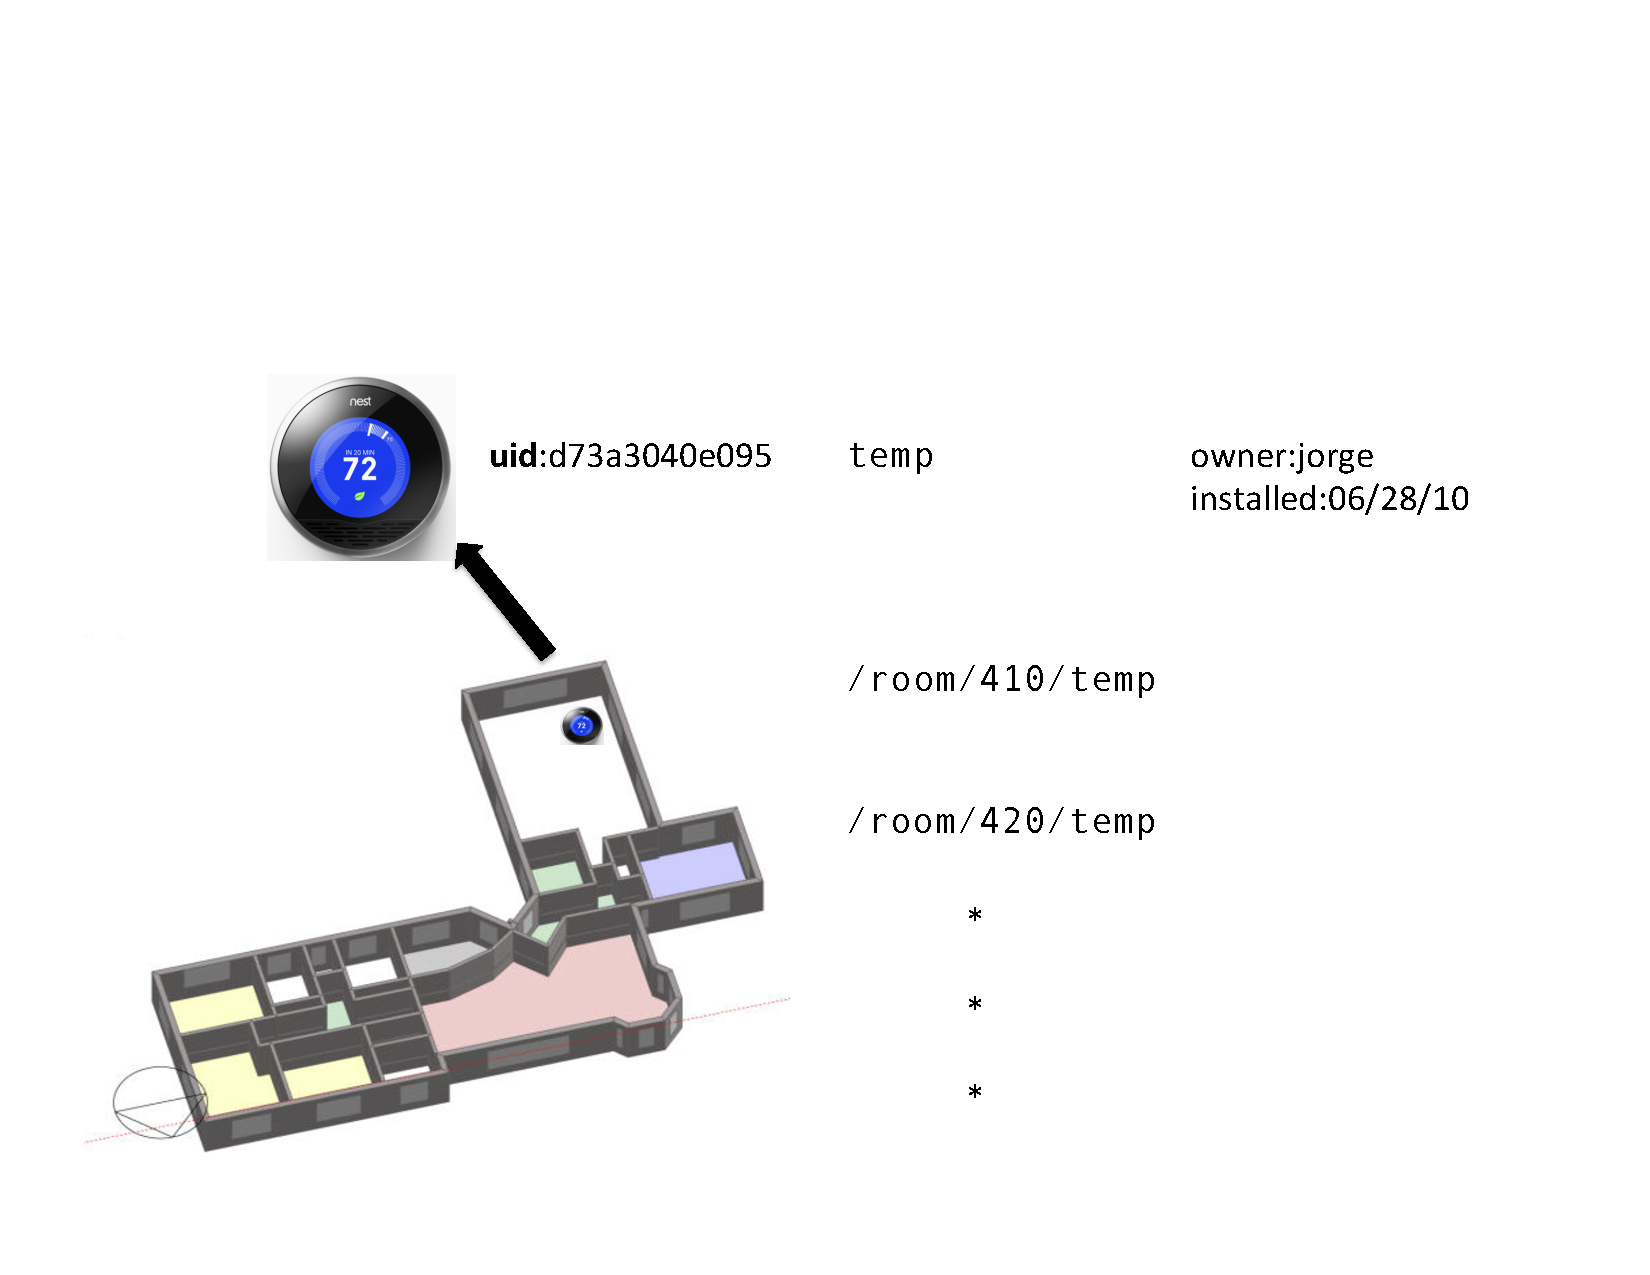
\includegraphics[width=0.65\columnwidth]{figs/everythingfile}
\caption{Everything is a file.  Temperature sensor represented as a file in a folder that contains folders for each room.
Note, the file that represents a temperature sensor producing a stream is given a unique identifer.  The user may also
decorate the file with extra metadata for searching purposes.}
\label{fig:everythingfile}
\end{figure}

In this example, the user is creating a temperature stream file in every room of the building.  The name of the file, given by the user,
is \emph{temp}.  Upon creation, the file is uniquely identified by the system using a unique identifier, as shown.  Like in a unix filesystem, the
file is created within a folder.  Ideally, the name of the folder would encode the placement of the sensor.  In the figure, the 
user is create a temperature stream file in room 410 and room 420.  Note the full filepath for the stream file is /room/410/temp.
During creation, the user may also decorate the file with extra metadata, also shown in the figure.  In this example, they have annotated
the file with information about the owner and when the sensor was installed.   This metadata is used for quickly locating the file
or grouping files that contain similar tags, quickly.

\subsection{File types and operations}
As we map the filesystem abstraction into this problem space, we need to consider the various kinds of files our system will contain,
their semantics, and how our system will expose and manage them.  There are essentially 4 types of files and 6 sub-types.  We summarize
these in Table~\ref{tab:filetypes}.  There are also different kinds of operations that the each file type supports.  Operational semantics
are file dependent.  For example, when you \emph{read} a folder, you obtain the metadata associated with the folder and the name
of its children.  When you \emph{read} a stream, you its metadata and the last timestamp-value it produced.  \emph{Writ}ing to a stream
is a bit different.  You can write to a stream to update its metadata tags and the stream source can write a value to it.  The stream
source is identified with a \emph{publish identifier} (pubid).  The stream source includes the pubid in the write operation for 
the specified stream file.  Without the pubid, the source cannot write to the file.  Any other writer should not be allowed to write to 
a stream file either.  

\begin{table}[h]
\begin{center}
\begin{tabular}{| r | l | l |}
	\hline
	\textbf{type} & \textbf{description} & \textbf{valid operations} \\ \hline
	default/folder & Container file.  Used to group other  & read, write, delete  \\
				   & kinds of files within it.  &  \\ \hline

	stream & Represents a data stream. & read, write, delete, subscribe, \\
			&							&query \\ \hline

	controller & Represents a controller. & read, write, subscribe \\ \hline

	special & There are several kinds of special files for  & read, delete \\
		    & management of jobs and pipes. &  \\ 
	\hline
\end{tabular}
\caption{Summary of the 4 main file types and their valid operations in StreamFS.}
\label{tab:filetypes}
\end{center}
\end{table}

Similar to a traditional filesystem, StreamFS includes \emph{special files}.  There are 6 special files and 5 of them 
are for management purposes.  The only one that is not is the \emph{symbolic link} file, which is essentially used to support
multi-naming and inherents the operational semantics of the file it points to.  The delete operation on a symlink, however,
only deletes the symlink.  A description of these files and the operations they support is given in Table~\ref{tab:filesubtypes}.
A detailed description and examples with be presented in later sections.


\begin{table}[h]
\begin{center}
\begin{tabular}{| r | l | l |}
	\hline
	\textbf{operation} & \textbf{file type} & \textbf{semantics} \\ \hline
	read & folder, stream, ipd, ipi, epd, epi, sub & read the metadata and tags for \\
		 &										   & the associated file. \\ \hline
	write &  stream & Write to stream file, only the \\ 
		  & 		& appropiate stream source is permitted.\\ \hline
	delete & folder, stream, ipd, ipi, epd, epi, sub & Folder must be empty.  \\
		   & 										 & The others can be directly deleted. \\ \hline
	query &  stream, all & streams support time-range queries.  \\
		  &			     & All support metadata-tag queries.\\ \hline
	subscribe & stream & Forwards data from a stream to the\\
			  &		   & specified destination.\\
	\hline
\end{tabular}
\caption{File opertaitons, the file types that support them, and their general semantics.}
\label{tab:semantics}
\end{center}
\end{table}

\subsection{Default, Stream, and Controller Files}
% \subsection{Default/Folder Files}
A default or folder file serve primarily as a container for other kinds of files.  It is used to group together different kinds of file and
to represent a common attribute of the file within it.  For example, a default file is usually used to construct the spatial hierarchy.
Each file at the top level represents a floor, its children are also a set of default file, representing each of the rooms on that floor.
A default file cannot be deleted unless it is empty.

File that represent streams are called stream files.  They are tightly associated with the associated stream data in the timeseries data-store.
A user created a stream file and that associated stream ``writes'' to it in order to have its data saved.  StreamFS also forwards the
data to the \emph{subscription manager} in case any subscription sink has subscribed to this feed.  When a stream file is create an id is 
returned to the user.  This id must be used by the stream that wishes to push its data to StreamFS through this file.  If this id is incorrect
or not include, the write operation is rejected.

Because controllers accpet many kinds of input, we designed the the file that presents a controller similar to the external processing stub discussed
in section~\ref{sec:externalprocs}.  Writes to a controller file and forwarded directly to the control stub running at the controller itself or a proxy
machine that communicates with the controller.  Any reply is set as metadata in the controller file.  Controller files also an associated output stream.
If a controller process wishes to inform the process of internal state at the controller, it does so through the controller file output --
a stream file itself.  Table~\ref{tab:filetypes} lists the files in streamfs and the operations they support.  The operational semantics
are listed in Table~\ref{tab:semantics}.

% \subsection{Stream Files}

% \subsection{Controller Files}

\subsection{Special Files}
There are 6 types of special files.  In chapter~\ref{chap:ProcMngtSchedMain} we eluded to the various kinds of file that are created
when a user creates an internal or external file.  An internal process definition (ipd) file is created when the user
submits a script to StreamFS.  When a (set of) stream(s) is piped through the defintion file, an internal process instance (ipi) file
is created that represents the output of the process.  A subscription instance (sub) file is also created.  The sub file contains
information about which streams are feed the file, a reference to the ipi file, and statistics about the file.  If either
the sub file or the ipi file are deleted, the process ends.  The ipi file is also a stream file.  It can be used to pipe that
output of the process to another processes or to an external \texttt{URL}.

\begin{table}[h]
\begin{center}
\begin{tabular}{| l | l | l |}
	\hline
	\textbf{type} & \textbf{description} & \textbf{valid operations} \\ \hline
	
	internal process  & Javascript process definition.  & read, write, delete  \\ 
	defintion (ipd)   & 							    &	\\ \hline

	internal process  & Management file used for managing & read, delete \\
	instance (ipi)	  & active processing of this script. & \\ \hline

	external process  & Gives information about where an & read, write, delete \\
	definition (epd)  & external process lives. &\\ \hline

	external process  & An active processing stream to an  & read, write, delete \\
	instance (epi)	  & external process. &\\ \hline

	subscription instance & An instance of a subscription.  Contains & read, delete \\
				(sub) 	  & information about the subscription, &\\
								& such as source/sink and related statistics &\\ \hline
								
	symbolic link (symlink) & Similar to a symbolic link in Unix. & \\
	\hline
\end{tabular}
\caption{Summary of the 6 special-file sub-types and their valid operations in StreamFS.}
\label{tab:filesubtypes}
\end{center}
\end{table}

The same set of files are created when an external processes is defined and started.  When the client stub is started on the client
machines it creates an external procrocess definition file for each process that was listed in the configuration file for the stub on 
the client machine.  Similarly, when streams are piped to the defintion files, the client starts the processes on the client
and create their associated external process instance (epi) files.  Those files are also a sub-type of the stream file and can
be used to pipe the output to another process (internal or external) or an external \texttt{URL}.
Any subscription or pipe that is instantiated creates an associated sub file in the \texttt{/sub} directory.  These always contain information
about the subscription and kill the fowarding process when deleted.

Finally, we used symbolic link (symlinks) the same way they are used in a traditional filesystem.  They are also used to generalize
the inter-relationship structure in the ERG.  They are a crucial file in the support of multi-naming.

% \subsection{Special Files}

% \subsubsection{Internal Process Definition}
% \subsubsection{Internal Process Instance}
% \subsubsection{External Process Definition}
% \subsubsection{External Process Instance}
% \subsubsection{Subscription Instance}










\section{Supporting Multiple Names}

One of the goals of the naming scheme in StreamFS is to support multiple names for sensor and actuators.  The inclusion of symlinks 
provides this ability.  A file can be named and linked to from multiple hierarchies.  This allows applications to refer
to the same physical entity with a unique object id through multiple names.  It is also used by our pub-sub system when
the names are resolved and play a crucial role in \emph{dynamic aggregation}.

For example, a temperature sensor may have at least two names that are expose to the end user.  It may have a name that refers to 
it through the context of its spatial placement, such as \texttt{/soda/4F/410R/temp} and it may have a name that refers to it 
through the context of its association with a component in the HVAC system, such as \texttt{/soda/hvac/ahu1/vent1/temp}.  Either
of those are names that should access the same item and that item's associated data.  The underlying stream may actually write
the data to a stream file named \texttt{/strms/temp} and the other two names are just symlinks to this one.  

The pub-sub system uses these names when decided which data streams match a subscription topic.  For example, in a typical pub-sub system,
if a job wanted to subscribe to the temp stream, it would have to know the name \emph{a priori}, or simply pick a single name.
However, we support the notion of multi-topic stream tags.  So, if a subscriber request all the streams with the topic 
\texttt{/soda/4F/410R/*} and a data point is written to \texttt{/strm/temp}, the subscription manager would list all the aliases
for that name, which include \texttt{/soda/4F/410R/temp} and see that it matches the topic request for that subscription.

Notice how naming explicitly affects how we group sensors according to some hiearchical organization.  Some of those groupings
are physical associations with one another that are important to stay accurate.  Let's re-examine the example presented in
Section~\ref{sec:cntxtacc}.  We present the figure from that section again in Figure~\ref{fig:mpc_example2}.

% walk through the example and show how multinaming helps address this and 
% why it's important to get right -- that should lead us right into the next section with no problem.

\begin{figure}[h!] %htbp
\centering
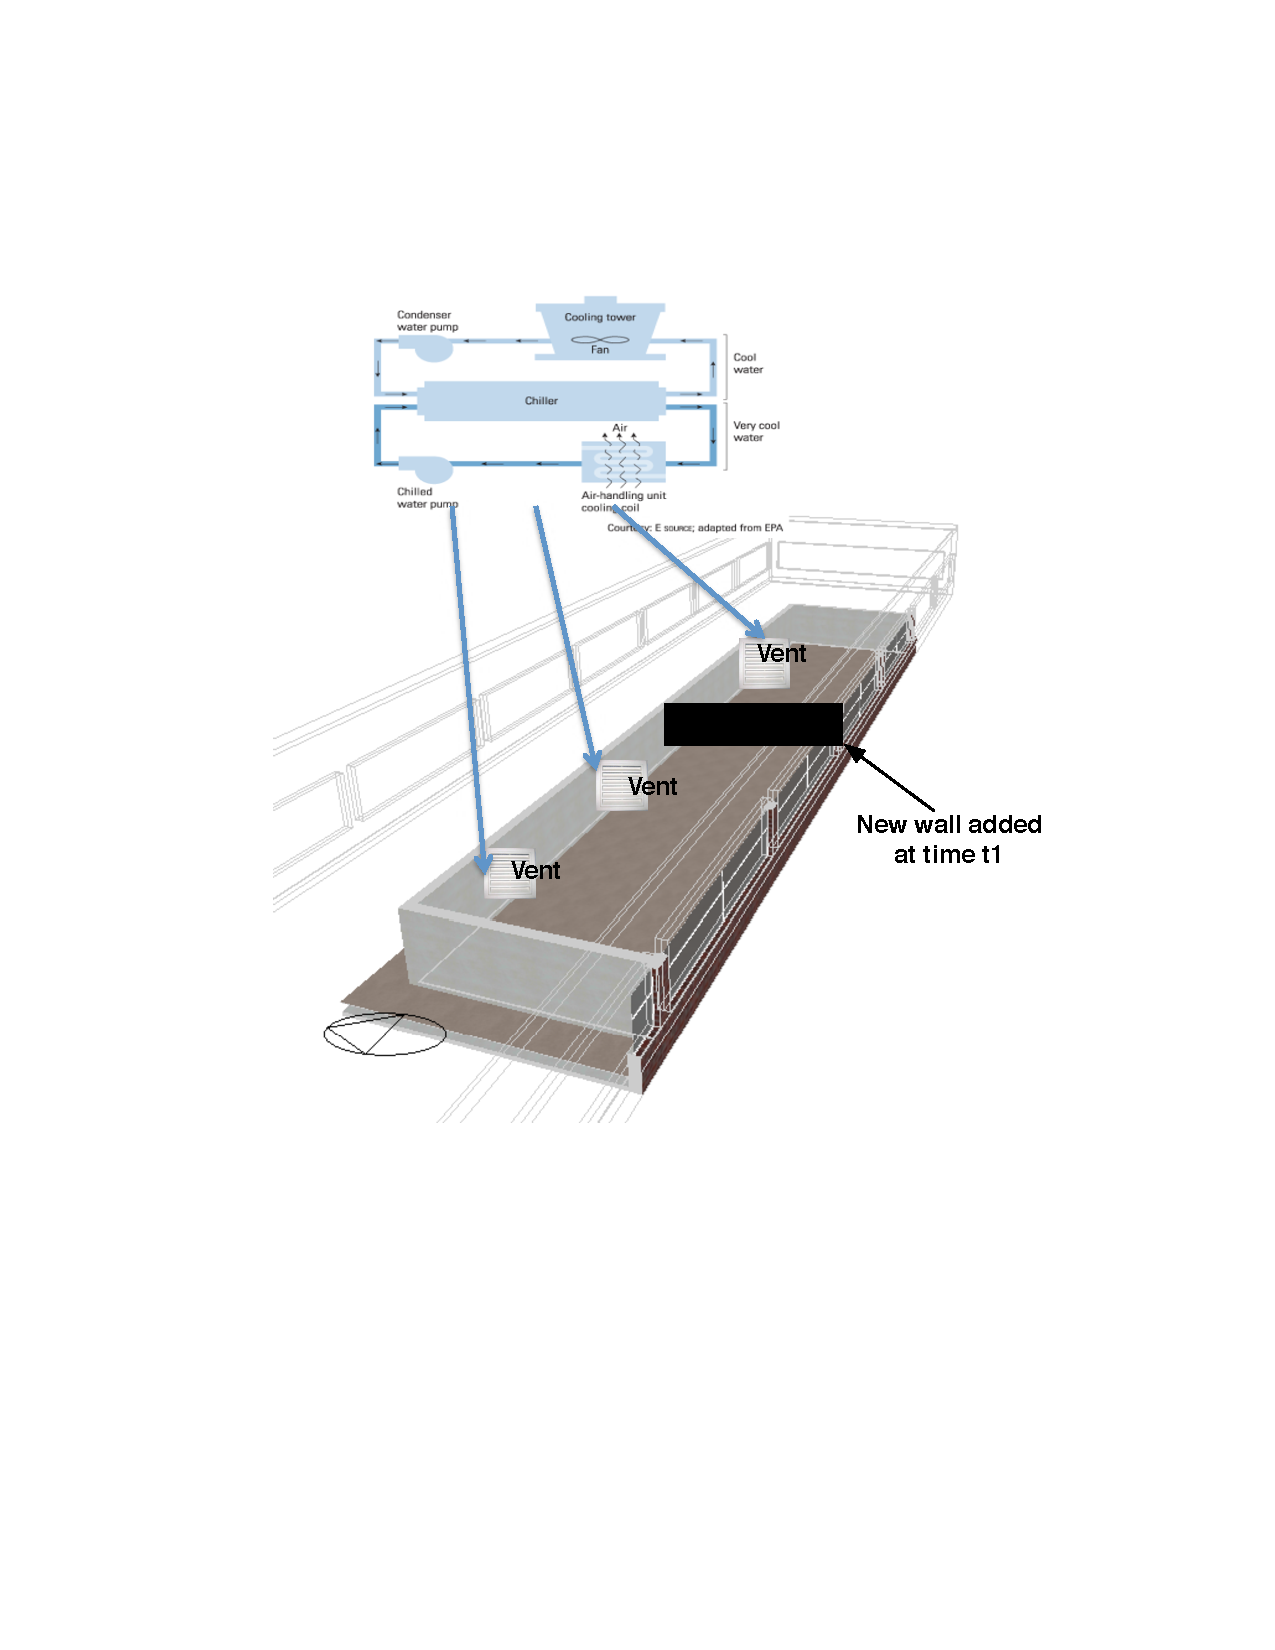
\includegraphics[width=0.5\columnwidth]{figs/mpc_example}
\caption{MPC example where metadata must be verified to maintain correct behavior.}
\label{fig:mpc_example2}
\end{figure}

Recall that the equation that drives the control process depends on knowing the mapping between vents and rooms.  Therefore,
if the room changes and a vent is added or removed, the control algorithm must be updated to account for the change.  The naming
structure would contain a reference to the vent in some group, linked to a sensor that belongs to a certain room, however,
if a wall is put up, we should be able to automatically detect that this has occurred to update the control process.
In summary, the naming scheme is used to express different kinds of organizational patterns for the sensors and their data.
As the building goes through some changes and evolves an automatic scheme or family of schemes are necessary to alert
the user or process of the chance.  In the next
section we discuss the mathematical tools we used to verify that the groups specified by the naming convention are correct.

\section{Verification through Sensor Data}
Verification is a broad topic in buildings that refers to verifying several things about building sensor metadata or through
the sensor data.  Both cases are related to physical states are relationships that are assumed by the user and are either
true and empirically observable or not.  If not, the end user or process should be informed and that inconsistencies should
be immediately addressed.  This is even more of an issues as building begin to reply more and more on software.

In this section we introduce some of the tools that we use for verification as discuss the 4 types of verification
that exists in buildings.  We also present an overview approach for 3 of them.

\subsection{Correlation}
Throughout this work, we make extensive use of the correlation coefficient function defined as: 

\begin{displaymath}
r(X,Y) = r_{X, Y} = \frac{\sum_{i=1}^{n} (X_{i} - \overline{X})(Y_{i} - \overline{Y})}
{\sqrt{\sum_{i=1}^{n} (X_{i} - \overline{X})^2}\sqrt{\sum_{i=1}^{n} (Y_{i} - \overline{Y})^2}}
\end{displaymath}

where $X$, $Y$ are separate sets of values, $n$ is the total number of sample points in 
each set, and $\overline{X}$ is the mean value of $X$ (same for $\overline{Y}$ and Y).  % over the entire sampling period.
For each pair of sensors, we compute the corrcoeff to ascertain the relationship between them.


\subsection{Empirical Mode Decomposition} \label{emd}
Another important tool that we used is empirical mode decomposition.  We use it partition the empiriical data is its constituent
sub-signals and examine what those sub-signals tell us about its behavior.  We also use it to examine how signal behavve between
one another at certain bands of importance that contain important physical information.

Empirical Mode Decomposition (EMD) \cite{huang:emd1998} is a technique that decomposes a signal and reveals intrinsic patterns, 
trends, and noise.
This technique has been widely applied to a variety of datasets, including climate variables~\cite{lee:climateEMD2011}, medical data~\cite{blanco:bioMed2008}, speech signals~\cite{huang:signalProc2006,hasan:ieeeletter2009}, and image processing~\cite{nunes:vision2005}.
% for example, it helped to uncover the global surface temperature trends\cite{}, solar activity patterns and predicts climate variables .
EMD's effectiveness relies on its empirical, adaptive and intuitive approach.
In fact, this technique is designed to efficiently decompose both non-stationary and non-linear signals without requiring any 
a priori basis functions or tuning.  

EMD decomposes a signal into a set of oscillatory components called intrinsic mode functions (IMFs). 
An IMF satisfies two conditions: (1) it contains the same number of extrema and zero crossings (or differ at most by one); (2) the two 
IMF envelopes defined by its local maxima and local minima are symmetric with respect to zero.  Consequently, 
 IMFs are functions that directly convey the amplitude and frequency modulations.

% EMD is an iterative sifting process that extracts IMFs step by step; each step seeks for the IMF with the highest frequency, then the computed IMF is removed from the data and the residual data are used as input for the next step.
EMD is an iterative algorithm that extracts IMFs step by step by using the so-called sifting process \cite{huang:emd1998}; each step seeks for the IMF with the highest frequency by sifting, then the computed IMF is removed from the data and the residual data are used as input for the 
next step.
The process stops when the residual data becomes a monotonic function from which no more IMF can be extracted.

We formally describe the EMD algorithm as follows: 
\begin{enumerate}
\item Sifting process: For a current signal $h_0=X$, let $m_0$ be the mean of its upper and lower envelopes as determined from a cubic-spline interpolation of local maxima and minima.
\item The estimated local mean $m_0$ is removed from the signal, giving a first component: $h_1 = h_0-m_0$
\item The sifting process is iterated, $h_1$ taking the place of $h_0$. Using its upper and lower envelopes, a new local mean $m_1$ is computed and $h_2 = h_1-m_1$.
\item The procedure is repeated $k$ times until $h_k=h_{k-1}-m_{k-1}$ is an IMF according to the two conditions above.
\item This first IMF is designated as $c_1 = h_k$, and contains the component with shortest periods. We extract it from the signal to produce a residual: $r_1 = X - c_1$.  Steps 1 to 4 are repeated on the residual signal $r_1$, providing IMFs $c_j$ and residuals $r_j  = r_{j-1}-c_j$, for $j$ from $1$ to $n$.
\item The process stops when residual $r_n$ contains no more than 3 extrema.
\end{enumerate}

The result of EMD is a set of IMFs $c_i$ and the final residue $r_n$, such as: \[X=\sum^{n}_{i=1}c_i+r_n\]
where the size of the resulting set of IMFs ($n$) depends on the original signal $X$ and $r_n$ represents the trend of 
the data (see \emph{IMFs} in Figure~\ref{fig:diagram1}).

For this work we implemented a variant of EMD called Complete Ensemble EMD~\cite{torres:icassp2012}.
This algorithm computes EMD several times with additional noise, it allows us to efficiently analyze signals that have 
flat sections (i.e. consuming no electricity in our case). % and permits us to solve the \emph{EMD mode mixing problem}.

\subsection{Reaggregation of Intrinsic Mode Functions} \label{methodo:corr}
By applying EMD to energy consumption signals we obtain a set of IMFs that precisely describe the devices consumption 
patterns at different frequency bands.  Therefore, we can focus our analysis on the smaller time scales, ignoring the dominant 
patterns that prevent us from effectively analyzing raw signals.

However, comparing the IMFs obtained from different signals is also not trivial,
 because EMD is empirically uncovering IMFs from the data there is no guarantee that the two IMFs $c_i^1$ and $c_i^2$ obtained from two distinct signals $S^1$ and $S^2$ represent data at the same frequency domain.
Directly comparing $c_i^1$ and $c_i^2$ is meaningless unless we confirm that they belong to the same frequency domain.

There are numerous techniques to retrieve IMF frequencies~\cite{huang:aada2009}.  
In this work we take advantage of the Generalized Zero Crossing (GZC)~\cite{huang:patent2006} because it is a simple and robust 
estimator of the instantaneous IMF frequency \cite{huang:aada2009}.
GZC is a direct estimation of IMF instantaneous frequency using critical points defined as the zero crossings and local extrema 
(round dots in Figure~\ref{fig:gzc}).
Formally, given a data point $p$, GZC measures the quarter ($T_4$), the two halves ($T_2^x$), and the four full periods ($T_1^y$), $p$   
belong to (see Figure~\ref{fig:gzc}) and the instantaneous period is computed as:
\[T=\frac{1}{7}\{4T_4+(2T_2^1+2T_2^2)+(T_1^1+T_1^2+T_1^3+T_1^4)\}\]

\begin{figure}
\begin{center}
 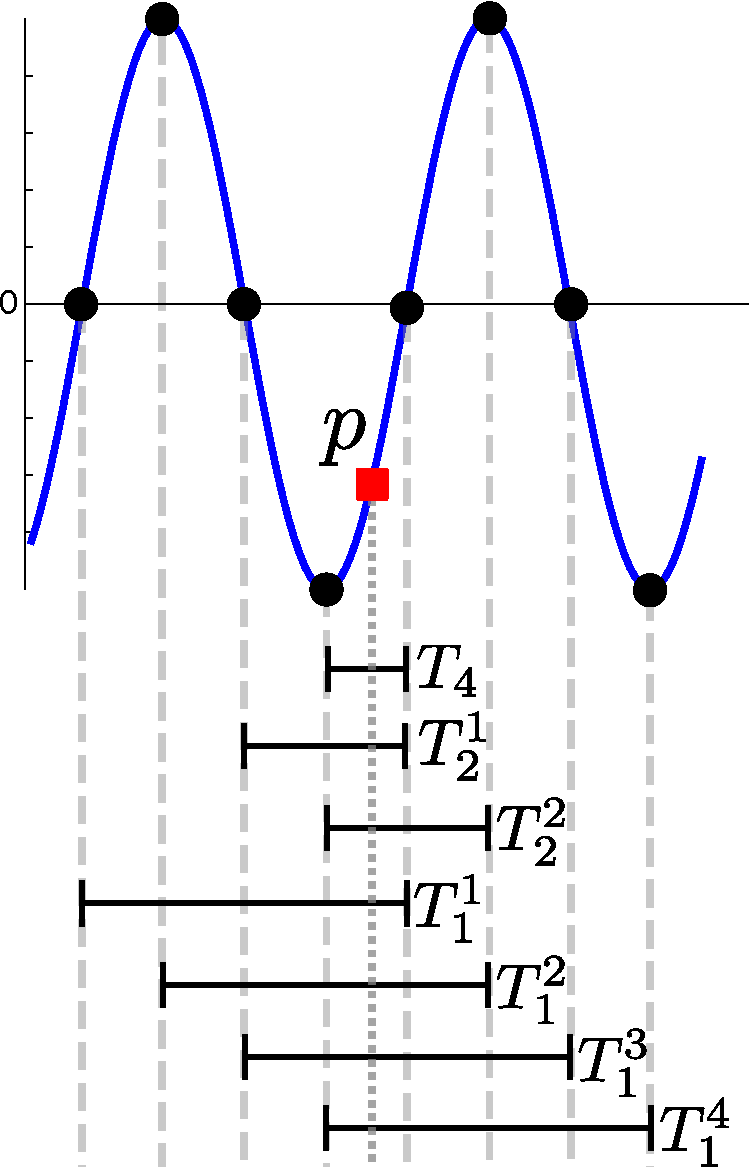
\includegraphics[width=.25\textwidth]{figs/gzc.pdf}
 \end{center}
 \caption{Generalized Zero Crossing: the local mean period at the point $p$ is computed from one quarter period $T_4$, two half periods $T_2^x$ and four full periods $T_1^y$ (where $x=1, 2$, and, $y=1,2,3,4$).}
 \label{fig:gzc}
\end{figure}

Since all points $p$ between two critical points have the same instantaneous period GZC is local down to a quarter period.
Hereafter, we refer to the time scale of an IMF as the average of the instantaneous periods along the whole IMF.
Because the time scale of each IMF depends on the original signal, we propose the following to efficiently compare IMFs from different signals.
We cluster IMFs with respect to their time scales and partially reconstruct each signal by aggregating its IMFs from the 
same cluster.  Then, we directly compare the partial signals of different devices.

EMD yields distinct components in different time scales and we compute the instantaneous frequencies \cite{IF} of IMFs using Generalized Zero-Crossing \cite{GZC}.  We break the time scales into four frequency bands:
\begin{itemize}
\item High Frequency: a time scale smaller than 30 minutes, mainly reflecting the operation characteristics of devices and noise in system. 
\item Medium Frequency: a time scale between 30 minutes and 6 hours, which is within the time span of daily activities inside a building.
\item Low Frequency: a time scale between 6 hours and 7 days. %This category usually captures patterns repeated in a longer cycle, say, days. 
\item Residue: everything has a time scale longer than 7 days and shows long-term patterns, such as seasonal changes.
\end{itemize}

Later in this thesis we will explain how we use the medium-frequency band for both spatial verification and functional verification.  We discuss
the 4 types of verification in the next section.






\section{Types of Verification}
There are 3 kinds of verification that we discuss in this section.

\begin{enumerate}
\item \emph{Functional}: verifying whether the behavior of the components in changing.
\item \emph{Spatial}: 	verifying the spatial relationship between components.
\item \emph{Categorical}: verifying the unit of measure and phenomenon being observed.
% \item Value
\end{enumerate}

Before we discuss the details and approach for each, let us first examine the mathematical tools that we
use in our solutions.  Then we discuss each type of verification in more detail.  We give a detailed description 
of the methodology for each and present the results of our analysis.

\subsection{Correlation}
Throughout this work, we make extensive use of the correlation coefficient function defined as: 

\begin{displaymath}
r(X,Y) = r_{X, Y} = \frac{\sum_{i=1}^{n} (X_{i} - \overline{X})(Y_{i} - \overline{Y})}
{\sqrt{\sum_{i=1}^{n} (X_{i} - \overline{X})^2}\sqrt{\sum_{i=1}^{n} (Y_{i} - \overline{Y})^2}}
\end{displaymath}

where $X$, $Y$ are separate sets of values, $n$ is the total number of sample points in 
each set, and $\overline{X}$ is the mean value of $X$ (same for $\overline{Y}$ and Y).  % over the entire sampling period.
For each pair of sensors, we compute the corrcoeff to ascertain the relationship between them.


\subsection{Empirical Mode Decomposition} \label{emd}
Another important tool that we used is empirical mode decomposition.  We use it partition the empirical data is its constituent
sub-signals and examine what those sub-signals tell us about its behavior.  We also use it to examine how signals behave between
one another at certain bands of importance that contain important physical information.

Empirical Mode Decomposition (EMD) \cite{huang:emd1998} is a technique that decomposes a signal and reveals intrinsic patterns, 
trends, and noise.
This technique has been widely applied to a variety of datasets, including climate variables\cite{climate}, medical 
data\cite{blanco:bioMed2008}, speech signals\cite{huang:signalProc2006,hasan:ieeeletter2009}, and image processing~\cite{nunes:vision2005}.
% for example, it helped to uncover the global surface temperature trends\cite{}, solar activity patterns and predicts climate variables .
EMD's effectiveness relies on its empirical, adaptive and intuitive approach.
In fact, this technique is designed to efficiently decompose both non-stationary and non-linear signals without requiring any 
a priori basis functions or tuning.  

EMD decomposes a signal into a set of oscillatory components called intrinsic mode functions (IMFs). 
An IMF satisfies two conditions: (1) it contains the same number of extrema and zero crossings (or differ at most by one); (2) the two 
IMF envelopes defined by its local maxima and local minima are symmetric with respect to zero.  Consequently, 
 IMFs are functions that directly convey the amplitude and frequency modulations.

% EMD is an iterative sifting process that extracts IMFs step by step; each step seeks for the IMF with the highest frequency, then the computed IMF is removed from the data and the residual data are used as input for the next step.
EMD is an iterative algorithm that extracts IMFs step by step by using the so-called sifting 
process \cite{huang:emd1998}; each step seeks for the IMF with the highest frequency by sifting, then 
the computed IMF is removed from the data and the residual data are used as input for the 
next step.
The process stops when the residual data becomes a monotonic function from which no more IMF can be extracted.

We formally describe the EMD algorithm as follows: 
\begin{enumerate}
\item Sifting process: For a current signal $h_0=X$, let $m_0$ be the mean of its upper and lower envelopes as determined from a cubic-spline interpolation of local maxima and minima.
\item The estimated local mean $m_0$ is removed from the signal, giving a first component: $h_1 = h_0-m_0$
\item The sifting process is iterated, $h_1$ taking the place of $h_0$. Using its upper and lower envelopes, a new local mean $m_1$ is computed and $h_2 = h_1-m_1$.
\item The procedure is repeated $k$ times until $h_k=h_{k-1}-m_{k-1}$ is an IMF according to the two conditions above.
\item This first IMF is designated as $c_1 = h_k$, and contains the component with shortest periods. We extract it from the signal to produce a residual: $r_1 = X - c_1$.  Steps 1 to 4 are repeated on the residual signal $r_1$, providing IMFs $c_j$ and residuals $r_j  = r_{j-1}-c_j$, for $j$ from $1$ to $n$.
\item The process stops when residual $r_n$ contains no more than 3 extrema.
\end{enumerate}

The result of EMD is a set of IMFs $c_i$ and the final residue $r_n$, such as: \[X=\sum^{n}_{i=1}c_i+r_n\]
where the size of the resulting set of IMFs ($n$) depends on the original signal $X$ and $r_n$ represents the trend of 
the data (see \emph{IMFs} in Figure~\ref{fig:diagram1}).

For this work we implemented a variant of EMD called Complete Ensemble EMD~\cite{torres:icassp2012}.
This algorithm computes EMD several times with additional noise, it allows us to efficiently analyze signals that have 
flat sections (i.e. consuming no electricity in our case). % and permits us to solve the \emph{EMD mode mixing problem}.

\subsection{Reaggregation of Intrinsic Mode Functions} \label{methodo:corr}
By applying EMD to energy consumption signals we obtain a set of IMFs that precisely describe the devices consumption 
patterns at different frequency bands.  Therefore, we can focus our analysis on the smaller time scales, ignoring the dominant 
patterns that prevent us from effectively analyzing raw signals.

However, comparing the IMFs obtained from different signals is also not trivial,
 because EMD is empirically uncovering IMFs from the data there is no guarantee that the two IMFs $c_i^1$ and $c_i^2$ obtained from two distinct signals $S^1$ and $S^2$ represent data at the same frequency domain.
Directly comparing $c_i^1$ and $c_i^2$ is meaningless unless we confirm that they belong to the same frequency domain.

There are numerous techniques to retrieve IMF frequencies~\cite{IF}.  
In this work we take advantage of the Generalized Zero Crossing (GZC)~\cite{GZC} because it is a simple and robust 
estimator of the instantaneous IMF 
frequency\cite{IF}.
GZC is a direct estimation of IMF instantaneous frequency using critical points defined as the zero crossings and local extrema 
(round dots in Figure~\ref{fig:gzc}).
Formally, given a data point $p$, GZC measures the quarter ($T_4$), the two halves ($T_2^x$), and the four full periods ($T_1^y$), $p$   
belong to (see Figure~\ref{fig:gzc}) and the instantaneous period is computed as:
\[T=\frac{1}{7}\{4T_4+(2T_2^1+2T_2^2)+(T_1^1+T_1^2+T_1^3+T_1^4)\}\]

\begin{figure}
\begin{center}
 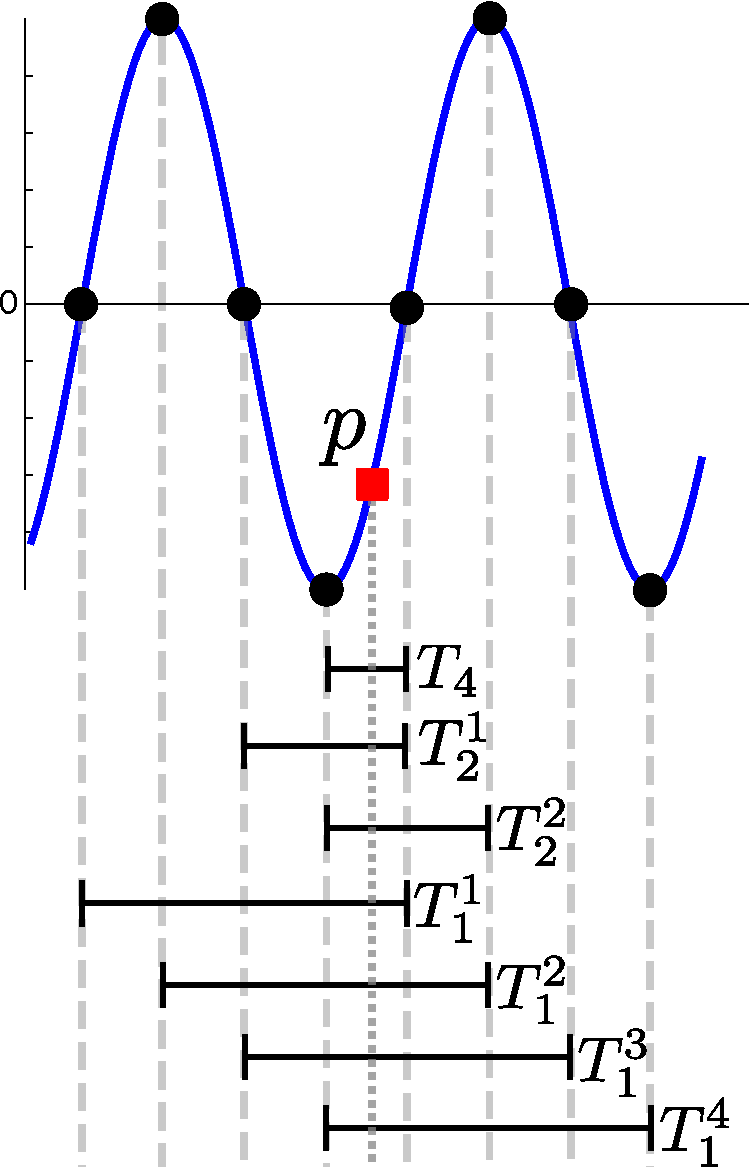
\includegraphics[width=.25\textwidth]{figs/gzc.pdf}
 \end{center}
 \caption{Generalized Zero Crossing: the local mean period at the point $p$ is computed from one quarter period $T_4$, two half periods $T_2^x$ and four full periods $T_1^y$ (where $x=1, 2$, and, $y=1,2,3,4$).}
 \label{fig:gzc}
\end{figure}

Since all points $p$ between two critical points have the same instantaneous period GZC is local down to a quarter period.
Hereafter, we refer to the time scale of an IMF as the average of the instantaneous periods along the whole IMF.
Because the time scale of each IMF depends on the original signal, we propose the following to efficiently compare IMFs from different signals.
We cluster IMFs with respect to their time scales and partially reconstruct each signal by aggregating its IMFs from the 
same cluster.  Then, we directly compare the partial signals of different devices.

EMD yields distinct components in different time scales and we compute the instantaneous frequencies \cite{IF} of IMFs using Generalized Zero-Crossing \cite{GZC}.  We break the time scales into four frequency bands:
\begin{itemize}
\item High Frequency: a time scale smaller than 30 minutes, mainly reflecting the operation characteristics of devices and noise in system. 
\item Medium Frequency: a time scale between 30 minutes and 6 hours, which is within the time span of daily activities inside a building.
\item Low Frequency: a time scale between 6 hours and 7 days. %This category usually captures patterns repeated in a longer cycle, say, days. 
\item Residue: everything has a time scale longer than 7 days and shows long-term patterns, such as seasonal changes.
\end{itemize}

Later in this thesis we will explain how we use the medium-frequency band for both spatial verification and functional verification.  We discuss
the 4 types of verification in the next section.







\subsection{Functional Verification}% With Strip, Bind, and Search}
% A typical large building contains thousands of sensors, monitoring the HVAC system, lighting, and other operational sub-systems.
With an increased push for operational efficiency, operators are relying more on historical data processing to uncover opportunities for energy-savings.
However, they are overwhelmed with the deluge of data and seek more efficient ways to identify potential problems.
In this thesis, we present an approach called the Strip, Bind and Search (SBS); a method for uncovering abnormal 
equipment behavior and in-concert usage patterns.
SBS uncovers relationships between devices and constructs a model for their usage pattern relative to other devices.
It then flags deviations from the model. 
% Unlike other approaches, SBS requires no a priori knowledge about the building.


The intuition behind the proposed approach is that each service provided by the building requires a minimum subset of devices.
The devices within a subset are used at the same time when the corresponding service is needed and a savings opportunity is characterized by the partial activation of the devices.
For example, office comfort is attained through sufficient lighting, ventilation, and air conditioning.
These are controlled by the lighting and HVAC (Heating, Ventilation, and Air Conditioning) system.
%controlled by the lighting system and air conditioner.% the light and air conditioning.
Thus, when the room is occupied both the air conditioner (heater on a cold day) and lights are used together and should be turned off 
when the room is empty.
In principle, if a person leaves the room and turns off \emph{only} the lights then the air conditioner (or heater) is a source of electricity waste.

Following this basic idea we propose \emph{Strip, Bind and Search} (SBS), an unsupervised methodology that systematically detects electricity waste.
Our proposal consists of two key components:
% \begin{enumerate}
%  \item The strip and bind method (SBM) mines raw sensor data, identifying devices that are used in concert.
%  It uncovers the devices relationships by looking at the correlation of their activities. 
%  Therefore it allows us to differentiate the devices that are used all together (high correlation), devices used independently (no correlation) and the mutually exclusive usages of devices (negative correlation).
%  \item The anomaly detector monitors devices relationships over time and reports misbehaving devices.
%  It learns the devices normal usages using a robust and longitudinal analysis of the building data and detect anomalous usages that stand for electricity wastes.
% \end{enumerate}

\begin{description}
 \item[Strip and Bind] The first part of the proposed method mines the raw sensor data, identifying inter-device usage patterns. % that are typically used in concert to provide a service.
We first \emph{strip} the underlying traces of occupancy-induced trends.  Then we \emph{bind} devices  whose underlying behavior is highly correlated. %, by placing them into a correlated device set.
 %  Then
 % It uncovers the devices relationships by looking at the correlation of their activities. 
 This allows us to differentiate between devices that are used together (high correlation), used independently (no correlation), and used mutually exclusively (negative correlation).
 \item[Search] The second part of the method monitors devices relationships over time and reports deviations from the norm.  % misbehaving devices.
 It learns the normal inter-device usage using a robust, longitudinal analysis of the building data and detect anomalous usages.  Such abnormalities usually present an opportunity to reduce electricity waste or events that deserve careful attention (e.g. faulty device).
 % that may represent that stand for electricity wastes.
\end{description}

SBS overcomes several challenges.  First, 
%The main challenge we overcame with our approach is uncovering the device relationships from numerous, 
noisy sensor traces that all share a similar trend, making direct correlation analysis non-trivial.
%The main difficulty in this approach is to uncover the devices relationship from the numerous and noisy sensor traces. 
Device energy consumption is mainly driven by occupancy and weather, all the devices display a similar daily pattern, in 
roughly overlapping time intervals and phases.
%and seem to be used all at once.
Therefore, one of the main contributions of this work is uncovering the intrinsic device relationships by filtering out the 
dominant trend.  For this task we use 
%% Romain
%This is achieved using a signal processing technique that exhibit the inherent characteristics of time series data, the 
Empirical Mode Decomposition \cite{huang:emd1998}, a known method for de-trending time-varying signals.
%% Romain

Another key contribution of this work is in using SBS to practically monitor building energy consumption.
Moreover, the proposed method is easy to use and functions in any building, as it does not require prior knowledge of the building nor extra sensors.  
It is also tuned through a single intuitive parameter.  %which parameter?

% In the rest of this paper, we detail the mechanisms of SBS (Section \ref{methodo}) before evaluating it with real data (Section \ref{eval}) then we discuss different outcomes of the proposed methodology (Section \ref{discussion}) and conclude.


\subsection{Spatial Verification}

Typically, placement information is embedded in the name or associated metadata for each sensor in the building.
These are used to group sensors by location.  For example, in our building data, all sensors that contain the string
 `410' in their name are in room 410.  Processes typically group streams in this fashion: using regular-expression matching 
or field-matching queries on the characters in the sensor name or metadata.  If these are not updated to reflect changes
then such group-by query results will not accurately represent true spatial relationships.  
% Fontugne et al.~\cite{IOT}
We observe that spatial associations can be derived empirically.  We start with this approach in our 
work and explore, more deeply, the extent to which it can be used 
as a verification tool for corroborating the groups constructed from character-matching queries.  We refer
to this process as \emph{spatial verification}.


\begin{figure*}[ht!]
\centering
    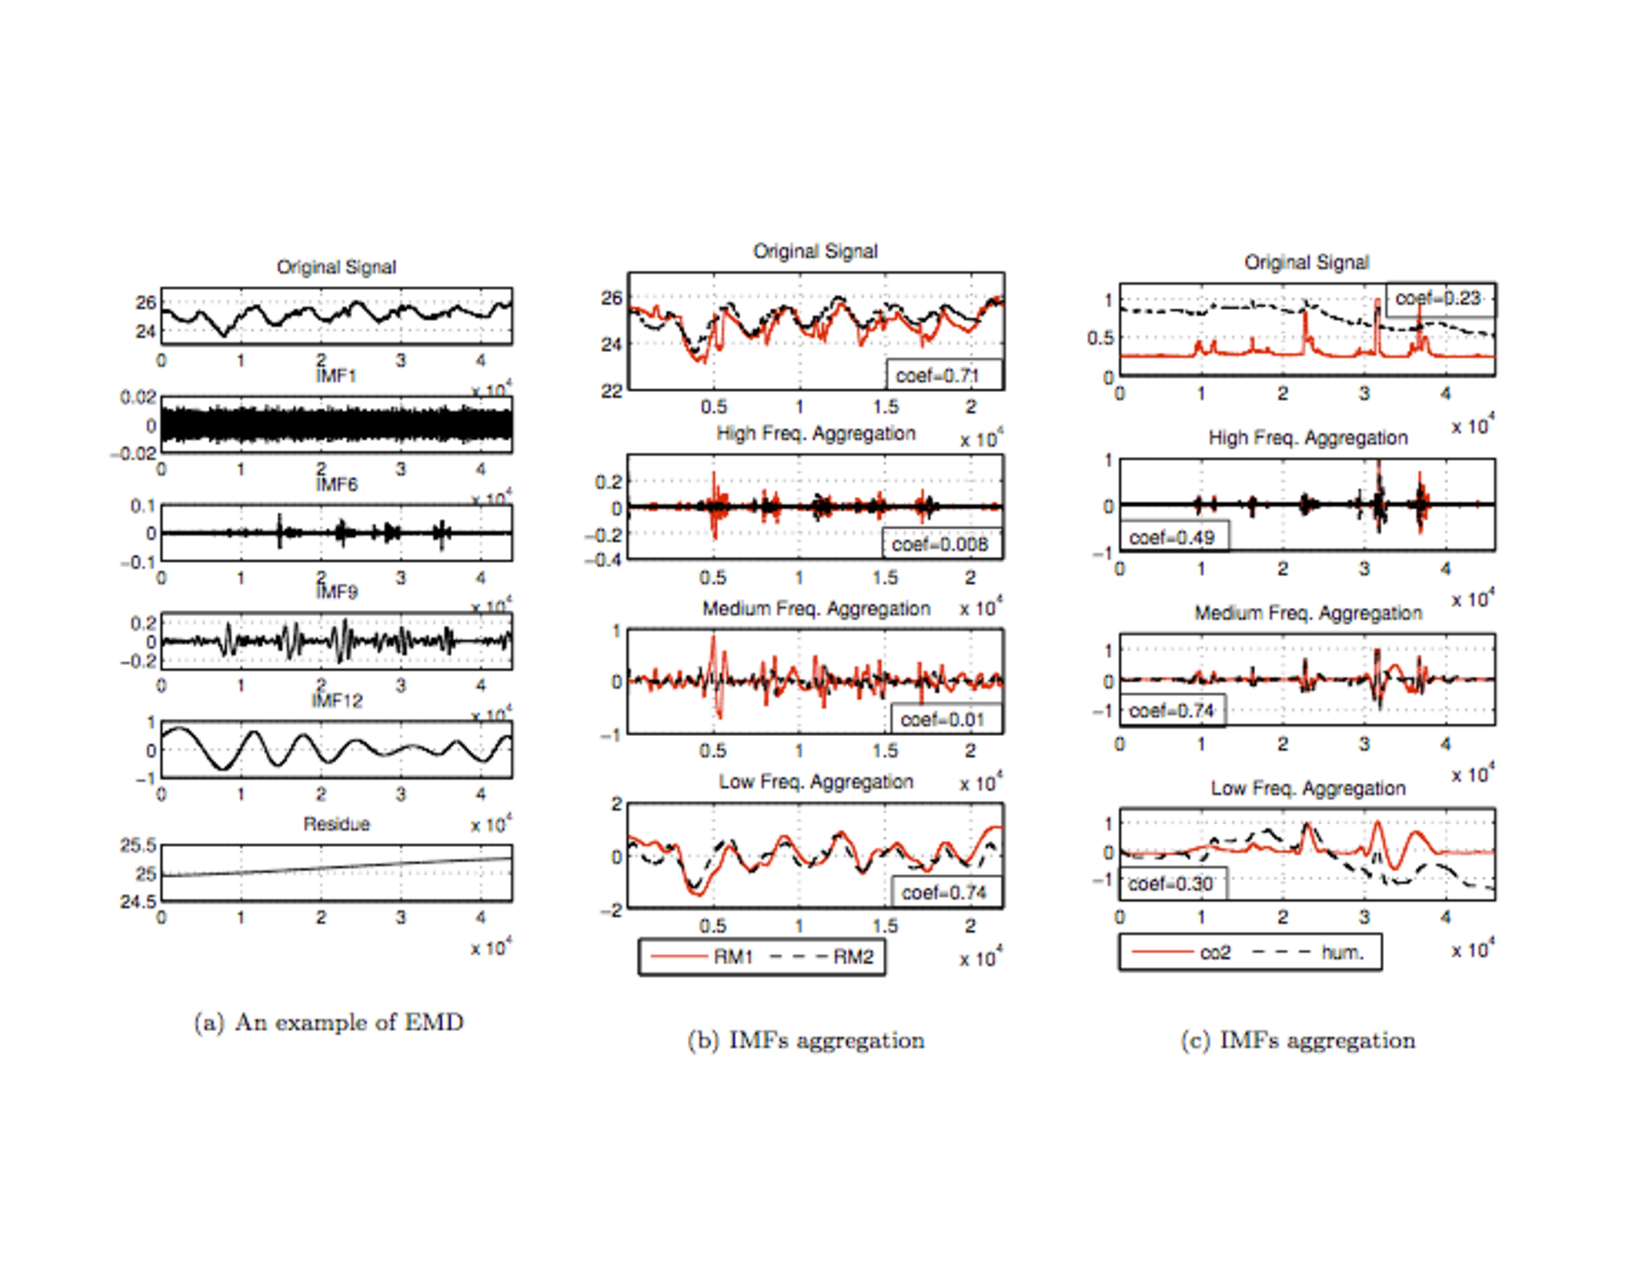
\includegraphics[width=0.95\textwidth]{figs/IMFReAggExample}
\caption{(a) EMD decomposes a signal and exposes intrinsic oscillatory components; (b) Aggregation of IMFs within a pre-defined frequency range makes seemingly similar signals from different locations more distinguishable; (c) IMF aggregation makes seemingly distinct signals of different sensors in the same room show high correlation.}
\end{figure*}

% We investigate the utility of empirical mode decomposition (EMD) to identify intrinsically
% correlated usage patterns among sensors in a large deployment.  We use data collected from almost $700$
% sensors in a 12-story building measuring power, pressure, temperature, and other physical
% phenomena.  We discover that doing a correlation analysis on the raw traces does not discriminate well enough
% to identify meaningful relationships between sensors.  We correlate the trace from a pump with the rest of
% the sensor traces and find that simple correlation filters only $50\%$ of the sensors as being correlated
% with the behavior of the pump. 
% In contrast, by running the correlation analysis on the constituent frequencies extracted by
% the EMD process, we filter out over $99\%$ of the sensors as being correlated -- with the highest correlation coming 
% from sensors that serve the same room as the pump.  We believe our approach can be used to 
% construct inter-device correlation models that can help understand and identify misbehaving or inefficient
% usage patterns.

% We present results for correlating usage patterns across a large number of sensors
% in a single deployment.  We analyze data from a 12-story office building at the University of Tokyo.  
% The deployment consists of almost 700 sensors monitoring a broad range of devices inside and outside 
% the building.  Our initial observations and results include the following:

% \begin{enumerate}
% \item Raw-trace correlation analysis is too strongly influenced by the common low-frequency trends in the data
% 	to identify meaningful relationships.
% \item Using a technique called empirical model decomposition (EMD)~\cite{huang:emd1998} removes this 
% 		 trend and helps identify truly correlated sensor traces.
% \item We can construct clusters of correlated sensors that are spatio-temporally correlated, \emph{without
% 		a priori knowledge of their placement}.
% \end{enumerate}



% Prior work~\cite{IOT} makes use of a technique called Empirical Mode Decomposition (EMD)~\cite{EMD} to statistically cluster correlated
% usage patterns.  Sensors close to each other show strong statistical correlations while sensors further apart show weaker correlations.  
% The main parameter in their approach, the correlation threshold, is explored to demonstrate how it relates to characteristic spatial patterns
%  in the sensor feeds.  However, they do not characterize the threshold as it relates to physical configuration.
% Fontugne et al.~\cite{SBS} expand the work by applying EMD to uncover functional device patterns.  They develop
% an unsupervised learning method to model normal usage patterns and apply an anomaly detection algorithm to alert when patterns
% have deviated from the norm.  The methodology used in their work divides raw signals into four separate frequency bands
% and shows the medium band to carry the most spatial information.

% In this section, we explore the threshold parameter in~\cite{IOT} more deeply, in order to move towards automatic spatial clustering, 
% to be used as a form of verification. We use EMD and the intrinsic mode function (IMF) re-aggregation methodology described in~\cite{SBS}, with some modifications, to statistically analyze the threshold parameter
% and its relationship to spatial separation in a building.  We explore the hypothesis that \emph{a statistical boundary, analogous to a physical one,
% exists and is empirically discoverable}.
% We conduct an empirical analysis on the data collected from 15 sensors in 5 rooms over a one-month period.  Our study makes the following contributions:

% \begin{itemize}
% \item We corroborate the results in~\cite{IOT}, verifying the spatial correlation pattern in a very different building.
% \item We characterize the correlation coefficient (corrcoeff) distribution of sensors in the same room and different rooms and validate our existence hypothesis for this preliminary sample.
% \item We demonstrate that the statistical boundary between sensors in various rooms converges to a similar value and this value generalizes across rooms in this study.
% \item We show the tradeoff between the true and false positive rate inherent to threshold selection. We also show that our method improves the classification accuracy from 80\% to 93.3\%.
% \end{itemize}

% Our results are promising yet preliminary.  We are able to find a statistical separation across a small number of rooms, quite well.
% Our study, however, does not explore the extent to which the physical separation affects the results.  Certainly for rooms that
% are far apart we observe a statistical distinction using our methodology.  However, we also find that in some cases, our approach
% does not work as well.  We discuss the approach and results in the rest of the paper, followed by a short discussion and future work.


We start our analysis by extending the methodology used for functional verification, based on empirical mode decomposition (EMD).  
In our analysis, we collect traces from several sensors and run EMD on them.  This produces a set of 
``intrinsic mode functions'' (IMF), which we separate by frequency range and re-aggregate them into distinct bands.
Then, we inspect the relationship between the sensors by computing the corrcoeff within a particular band, which 
gives us the spatial information we are interested in. 
Finally, we separate the result set into sub-sets, and closely examine their statistical characteristics. 
% Before describing our methodology in detail, we introduce some definitions and notation.



\subsection{Categorical Verification}
Categorical verification is the ability to cluster sensor traces by the type of sensor that it (i.e. its unit of measure) and the thing it is measuring.
Ideally we should be able to separate feeds that are measuring different physical attributes and/or are placed in different parts of the building.
For example, if there are sensors measuring temperature in a pipe and temperature in a room we should be able to separate them from one another as well
as separate them from sensor pressuring pressure in a valve.  We will show that this can be by examining their distribution and for 
small data sets with different sensor our approach works quite well, however we present some challenges in a large, more realistic deployment
data set and we discuss why it is so challenging to deal with.


% \subsection{Value Verification}
% Value verification used a physical model to verify that the value observed in the given context is producing values that agree with the model
% that is based on first-principles.  We do not explore this problem in this thesis and leave it for future work.


\section{Building Datasets}

In this thesis, we run all of our experiments and analysis on data from the four buildings.  They serve as 
the main sites for experiemental data collection and/or sites from which we obtained data dumps from their building
management system.

% In addition, we expect the anomaly detector to identify discontinuities in these relationships that represent obvious electricity saving opportunities (e.g. a room HVAC left on during night while the room lights have been turned off).

% Due to privacy concern this dataset is not publicly available on the Internet but accessible upon request.


\subsection{Engineering Building 2 - Todai}\label{data:engbldg2}
%The data from building 1 is collected at the Engineering Building 2 of the Hongo campus. 
Engineering building 2, at the University of Tokyo (Todai), is a 12-story building completed in 2005.  It contains
classrooms, laboratories, offices and server rooms.  
The electricity consumption of the lighting and HVAC systems of 231 rooms is monitored by 135 sensors.
Rather than a centralized HVAC system, small, local HVAC systems are set up throughout the buidling.  
The HVAC systems are classified into two categories, EHP (Electrical Heat Pump) and GHP (Gas Heat Pump).
The GHPs are the only devices that serve numerous rooms and multiple floors.  The 5 GHPs in the dataset serve 154 rooms.
The EHP and lighting systems serve only pairs of rooms and which are directly controlled by the occupants.
In addition, the sensor metadata provides device-type and location information (room number), 
therefore, the electricity consumption of each pair of rooms is separately monitored.


\section{Related work}

%\begin{itemize}
% \item dashboard
% \item andrew's lightin control work
% \item Kamin's hvac control work
% \item BEMs
% \item sMAP stuff
%\item Buildsys 2010 work~\cite{hbci}
%\item distributed consistency management: COPS
%\item mobility: tracking things with RFID~\cite{rfid_gonz2006}
%\item mobility: tracking of people, wifi indoor localization
%\item entity-relationship graphs
%\item homeOS [microsoft]
%\item HP Cooltown~\cite{cooltown}
%\end{itemize}
Our work touches on several areas from smart home research to logistics.  In the building space, there has been
some interest in building various kinds of energy-related visual and control applications.
This work focuses on the object definition, tracking, and management component of the architecture proposed by 
Hsu et al.~\cite{hbci}.  Their work stratefied the set of challenges that one could potentially face if the application 
were deployed at scale.  Our
work, in constrast, bases its design rationale on a \emph{real deployment} that is taking place at scale in a building 
on our campus.  We focus on solving fundamental systems challenges in dealing with intermittent connectivity
and conflict resolution in tracking people and things over time.  We also focus on leveraging gestures to minimize
the cost of interaction for users, while maximizing the information we can attain about the state of the world.

% Tracking people/indoor localization
An important aspect of the Energy Lens is determining when people and things have moved.  This requires some form 
of indoor localization.  There's a large body of literature in the area of indoor localization with mobile phones ranging from 
using wifi~\cite{radar}, to sonar~\cite{cricket}, to ambient noise~\cite{abs}, and a combination of sensors on the 
phone~\cite{surroundsense, darwinphone}.  Dita~\cite{dita} uses acoustic localization of mobile phones and also uses the infrastructure 
to determine gestures in free-space that are classified into pre-defined control actions.  Each of these require relatively complex 
software and/or infrastrure.  
We take a radically different, simple approach.  We use cheap, easy to re/produce tags (QR codes), place them on things in the 
environment over incrementally and use the natural \emph{swiping gesture} that users make, when interacting with the Energy Lens 
application, to track when they have moved or when the objects around them have moved.  The working principal is to attain as much 
information from their gesture to determine when something/one has moved.  We discuss our heuristics in section~\ref{sec:swipes}.

% context-aware apps
ACE~\cite{ACE} uses various sensors on the phone to infer a user's context.  The context domain consists of a set of user activities
and semantic locations.  For example, if ACE can distinguish between {\tt Running, Driving, AtHome, or InOffice}.  ACE also infers 
the one from the others, so if the user is {\tt AtHome} then they are not {\tt InOffice}.  Energy Lens uses inference to determine
when a person or thing has moved.  Certain swipe combinations give us information about whether they moved and where they moved to or
whether an item moved and where it moved to.  The main difference is that we only infer context when a user is actively swiping, rather
than a continuous approach.  Pretching is a fundamental technique used in many domains.  However, the cost of a prefetch for mobile
application outways the benefits if the prefetched data is not useful.  Informed mobile pretching~\cite{IMP} uses cost-benefit analysis 
to determine when to prefetch content for the user.  In the Energy Lens context, we prefetch data based on their location swipes.
We also rely on pretching to anticipate loss of connectivity, not just to improve preformance.

% Tracking things
Logistic systems focus on the tracking of objects as the move through distribution sites to warehouses, stores, shelves,
and purchase.  Items are tracked through bar code or RFID readers.  However, the workload is very structured and well
defined.  The authors of~\cite{rfid_gonz2006} describe this structure and leverage it to minimize storage
requirements and optimize query-processing performance.  Energy Lens uses the QR codes as the tag and the phone as an active
reader.  As objects move, users scan those items to their new location.  However, objects may belong to one or
many people, they can be metered by multiple meters a day, and their history in the system
is on-going.  In contrast, a typical logistics workload has a start (distribution site) and end point (leaving the store
after a sale).  In our workload, relationship semantics are important; we need to know whether the meter is \emph{bound-to}
rather than simple \emph{attached-to} an item.  We discuss the difference later in the paper.
% In addition to traditional logistics-style queries -- \emph{What is the average time that it took coffee-makers to move from the 
% warehouse to the shelf and finally to the checkout counter in January of 2004?} -- energy-analytics requires queries to group
% partial traces from meter data by tracking what meters the item attached to over the specified time-frame.
% The Energy Lens system collects and manages this kind of information to enable such queries.
Furthermore, we take advatange of natural gestures the user makes with the phone while scanning QR codes to extract
information about the current location of the user or things.

% Tagging items, virtual services
The key idea in the HP Cooltown~\cite{bridgingphysical,cooltown} work is to web-enable `things' in the world, grouped-by
`place', and accessed by `people' via a standardized acquisition protocol (HTTP) and format (HTML, XML).  
Cooltown creates a web presence for things in the world either directly (embedded web server) or indirectly 
(URL-lookup tag) as a web page page that display the services it provides.  Many of the core concepts in Cooltown 
also show up in Energy Lens.  The main overlap is the use of tags in the world that contain a reference to a virtual 
resource, accessible via HTTP through
a network connection.  Cooltown, however, explicitly chooses not maintain a centralized relationship
graph, it leverages the decentralized, linking structure of the web to group associated web pages together.
Furthermore, things are assumed to not move.  People are the main mobile entities.  The kind of applications
we wish to support must track where things are and their specific inter-relationships.  We imposed a richer set of 
semantics on our, centrally maintained, relationship graph and use it to provide detailed energy information.


\section{Summary}

% StreamFS consists of over 20,000 lines of code and was implemented in mostly Java.  It was deployed across multiple
% buildings and several applications were built on top of it over a 2 years period.

In this chapter we gave an overview of the main components in StreamFS.  Each of the components addresses the concerns stated in 
section~\ref{sec:shortcomings}.  The filesystem name server expose a uniform namespace for access sensors and actuators in 
deployed throughout the building.  The timeseries database serve to store data streaming physical information and 
is optimized for the scan-style queries posed by applications.  These address points \ref{nw} and \ref{ts}.
We also include a pub-sub system which serves multiple purposes.  It provides real-time data forwarding for external
applications and forwards data internally to processing units that are specified or linked by the user.
This addresses points \ref{rt}.  Finally, we introduce processing elements, both internal and external to address
point \ref{proc}.  We also introduce an entity-relationship graph to deal with indirect relationships that are
expressed in the construction of names in the system.

In the next chapter we talk more about processing and discuss the details in the scheduler that help enable applications
that have certain delivery requirement.



\chapter{Architectural Evaluation}
\label{chap:ArchEvalMain}

\section{API Overview}

In this section we give an overview of the application programming interface.  We provide a description of
function calls and the corresponding HTTP/REST version.  A full tutorial of the HTTP/REST interface can be found 
in Appendix~\ref{appendix:tutorial}.

\begin{table}[h]
\begin{center}
\begin{tabular}{| r | l |}
	\hline
	\textbf{function} & \textbf{description} \\ \hline
	create & Create a file. Overlaps with several other calls.    \\ \hline

	delete & Delete a file. \\ hline

	register & Join as data source.    \\ \hline

	push & Write to associated stream file.  \\ \hline

	label & Add an attribute-value pair.  \\ \hline

	rlabel & Remove an attribute-value pair.  \\ \hline
\end{tabular}
\caption{Overview of StreamFS file-related API calls.  Library written in Java, PHP, and C.}
\label{tab:api_calls1}
\end{center}
\end{table}

Table~\ref{tab:api_calls1} gives and overview of API calls that are available through the standard library, available in several
languages.  It provides functions for creating and deleting files as well as decorating them with attribute-value pairs.
The Energy Lens application makes extensive use of this library interface for dealing with consistency-management
features and ``atomic'' update operations.  Applications that run on the phone, typically use the HTTP/REST
interface.


\begin{table}[h]
\begin{center}
\begin{tabular}{| r | l |}
	\hline
	\textbf{callback} & \textbf{description} \\ \hline
	search & General search of terms through file name and content.  Similar to grep.    \\ \hline

	filter & Used to filter the returned list by attribute-value pair or path.    \\ \hline

	query & Timeseries query.    \\ \hline

\end{tabular}
\caption{Summary of control interface callbacks in StreamFS.  Library written in Java, PHP, and C.}
\label{tab:api_calls2}
\end{center}
\end{table}

The search API is simple (summarized in Table~\ref{tab:api_calls2}).  It includes three main calls, depending 
on what kind of data you are searching for.  
If the application wishes to make a general search based on the name of the file or the metadata it is decorated with, 
the \texttt{search} call allows you to specify 
a set of terms to look for or to specify specific attribute-value pairs.  It performs the search as a \emph{filter-forward}.
It uses provides a general \texttt{path} sub-option where you can specify that the path match a regular expression.
For example, \texttt{search(type:plug-load).path(/410/*)} returns all the files that contain the ``type:plug-load''
attribute-value pair in their metadata and \texttt{/410/} as a prefix for any of their names.  This example 
AND's the search criteria. 
The filter call can be combined with the search call to filter on metadata values returned from the \texttt{path} search.
For example, \\ \texttt{search(type:plug-load).path(/410/*).filter(owner:jorge)} 
fetches the same files as before but filters those that contain the attribute-value pair ``owner:jorge''.
Finally, the \texttt{query} call runs a timeseries query on a specified path or all stream files
that match a regular expression specified by through the \texttt{path} option.

The pub-sub library is used extensively in all our applications.  It is specifically used in 
the Energy Lens for initiating aggregation processing.  Table~\ref{tab:api_calls3} summarizes
the two main API calls for dealing with subscriptions and pipes.


\begin{table}[h]
\begin{center}
\begin{tabular}{| r | l |}
	\hline
	\textbf{callback} & \textbf{description} \\ \hline
	pipe & Pipes the list of specified streams to \\
		 & either an active process or a process \\
		 & definition file.    \\ \hline

	subscribe & Create an subscription from a 		 \\
			  & set of streams to an external target \\
			  & through a callback function. 		 \\ \hline

\end{tabular}
\caption{Summary of control interface callbacks in StreamFS.  Library written in Java, PHP, and C.}
\label{tab:api_calls3}
\end{center}
\end{table}

Internally, the mechanism for dealing with both is similar, however, the semantics of each call is differe.t % two calls implies that
Pipes direct streams to user-defined internal/external processing elements, while subscriptions are
for external sinks running on the client.  Subscriptions are managed through an \texttt{HTTP POST}
operation.  If the user is using a client stub, the \texttt{POST} is unmarshalled and a callback
is triggered with the body of the \texttt{POST} submission.

% \begin{table}[h]
% \begin{center}
% \begin{tabular}{| r | l |}
% 	\hline
% 	\textbf{callback} & \textbf{description} \\ \hline
% 	ctrlRcv & Function that handles the reception of control data.    \\ \hline

% 	remove & Informs device of removal.    \\ \hline

% 	suspend & Tells device to stop sending data.  \\ \hline

% 	resume & Tells device to resume sending data.  \\ \hline
% \end{tabular}
% \caption{Summary of control interface callbacks in StreamFS.  Library written in Java, PHP, and C.}
% \label{tab:api_calls2}
% \end{center}
% \end{table}

% Full RESTful tutorial is in the Appendix, 
\section{Deployment Viewer Application}

\begin{figure}[htb!]
\begin{center}
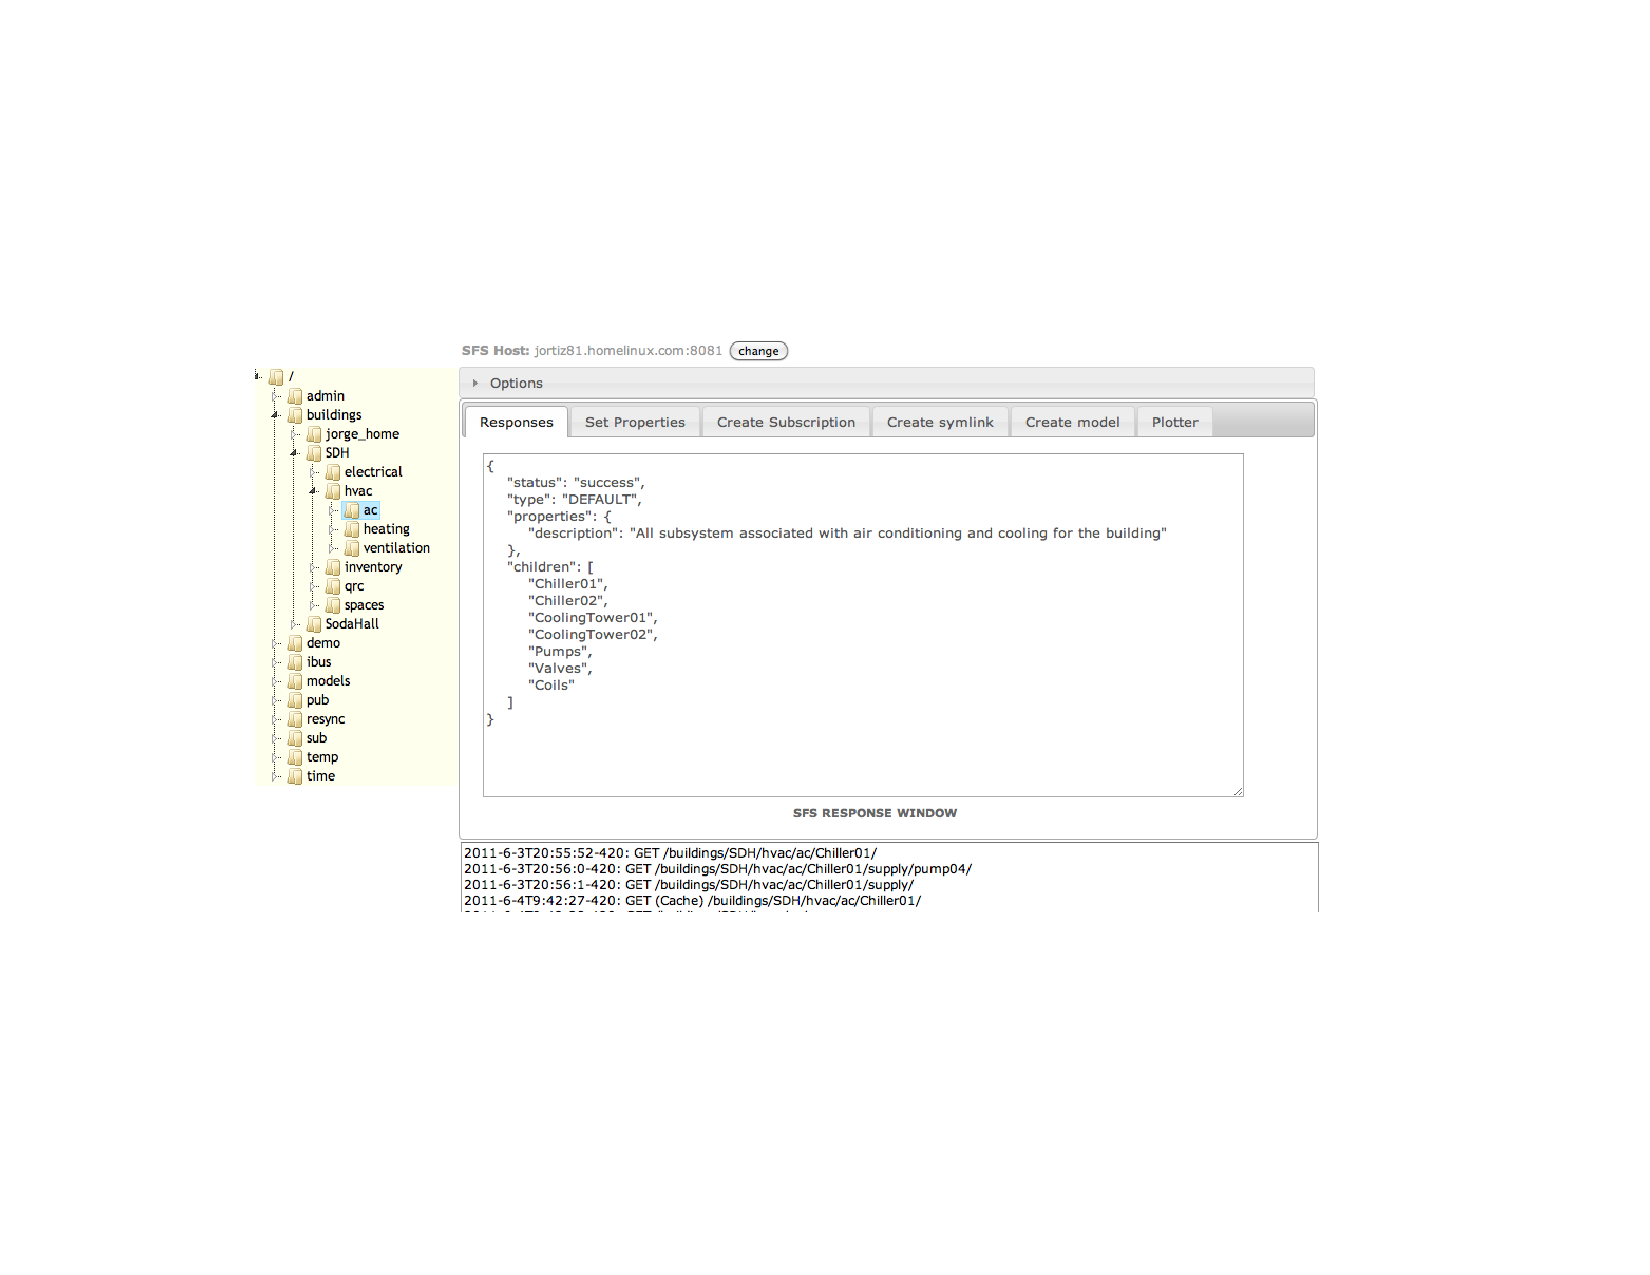
\includegraphics[scale=0.6]{figs/sfs_console}
\caption{StreamFS console.  The tool allows the user to view the namespace as a set of files, interact with the system, and 
view stream data.}
\label{fig:aggtree}
\end{center}
\end{figure}
\input{ArchitecturalEvaluation/MountedFSandMatlab}
\section{Visualization and Analysis of Streaming Data}



\section{Energy Auditing With Mobile Phones} 

Mobile phone penetration continues to rise and is predicted to reach 50 billion by 2020~\cite{mobile2020}.  As such, it is a ubiquitous,
powerful tool to serve as an interface between occupants and the built environment.  Mobile phones are constantly connected, 
are personal devices that can serve as a proxy for the individual, and provide large viewing screen for display of critical information
to its owner.  By combining the data streams available in the building with mobile phone, we could provide a way to
do in-situ diagnosis of opertional problem in the building, monitor personal energy consumption, and share information about
the building with our neighbors in the building.

There are several systems challenges that must be overcome in order to achieve this vision.
%One of the 
% We need to place live metering on plug loads.  We need to integrate data from the BMS with plug load and other
% meter data.  We need to be able to approximate the attribution algorithms and tailor them for real-time processing.
We examine those dealing capturing and maintaining a view of the physical world.  We must record which things belong to whom, 
where people
and things are over time, how to deal with the mobile phone as the main interactive modality, and how to do this at the scale of 
hundreds to thousands of users and meters.  We argue that \emph{without addressing these systems issues, this
vision cannot be achieved}.  In our work, we start by deploying a network of wireless power meters and use the mobile
phone to re-create a model of people, things, and locations in the building.  We also use it to assist in tracking of 
people and things over time.

% \subsection{Approach With StreamFS and Mobile Phones}
We use mobile phones to construct an entity-relationship 
graph of the physical world and combine it with streaming sensor data in order to perform detailed energy-attribution.
We limit the scope of the world to a single building domain.  We have designed and implemented a real-time, mobile energy auditing
application, called the `Energy Lens', that allows us to collect information about 
things throughout the building and how they are related to each other.  For example, computer X is inside 
room Y and connected to meter Z.  Then, we use these relationships to guide our data look-up and analytical
calculations.  For example, the load curve of room Y consists of the sum of all the power traces for loads
inside room Y.  We use the mobile smartphone as the main input tool.  Our work examines \emph{three main challenges} in setting up and 
deploying a real, whole-building infrastructure to support real-time, 
fined grained energy analytics.  

The first challenge is related to tracking and mobility.
The use of mobile phones presents classical, fundamental challenges related to mobility.  Typically, mobility
refers to the phone, as the person carrying it moves from place to place.  However, in the energy-attribution
context, we are also referring to the movement of energy-consuming objects.  Tracking their relationships to spaces 
and people is as important as tracking people.  We describe how we deal with \emph{both moving people and 
moving objects} and show that these historically difficult problems can be addressed relatively easily, if the proper infrastructure is 
in place.  %We provide evidence that the approach is simple, incrementally deployable, and scalable.

The second challenge is about capturing the inter-relationship semantics and having these inform our  analytics.
We adopt the general notion of physical tags that identify objects in the world.  Our system uses \emph{QR codes} to tag things and locations 
in the physical world.  However, \emph{any tag that provides a unqiue identifier for an object could serve the same purpose}.
Once tagged, there are three types of interactions -- 
registration, linking, and scanning -- which establish important relationships.  Registration is the act of creating a virtual object 
to represent a physical one.  Linking captures the relationship between pairs of objects.  Scanning is the act of performing an item-lookup.
Each of these interactions requires a set of swiping gestures.  Linking requires two tag swipes while the other two actions
require a single tag swipe.  Internally, we maintain a \emph{entity-relationship graph (ERG)} of things, people, and locations, that gets
updated through these sets of gestures.

The third challenge is about indoor network connectivity and access.
In order to connect these components, we rely on having `ubiquitous' network connectivity.  However, in practice, network
\emph{availability} is intermittent and our system must deal with the challenges of intermittency.  We discuss how caching
and logging are used to address these challenges.  Moreover, when connectivity is re-established, we must deal with
applying updates to the ERG, as captured by the phone while disconnected.  

Conflicts can also occur during an update.  For example, the two updates may disagree about which items are attached
to which meters.  We implement a very simple conflict resolution scheme, described in section~\ref{sec:conflicts}.
Finally, certain physical-state transitions are represented as a set of updates to the ERG that must be applied 
atomically.  We implement transactions in the log-replay and transaction manager.
Our `Energy Lens' system is deployed in a building on our campus.  We discuss
its architecture and our design choices.  
  
We also discuss novel strategies for tracking moving people/things and describe how we implement these in our system.  In summary, our work
makes the following contributions:

\begin{itemize}
\item We design and implement a system that captures and combines physical entities, their inter-relationships, and real-time sensor data 
		in buildings.% using mobile phones, qr code, and a cloud-based infrastructure.
\item We observe that certain combinations of swipes give us useful information to set the location of people and things over time.
		We codify this observation in our \emph{context-tracker} and use it to maintain consistency between the entity-relationship graph and the 
		state of the physical world.  To the best of our knowledge, this is radically different from the approaches in standard 
		localization techniques.  However, we argue that it can be used to \emph{enhance} their accuracy and overall performance.
\item We implement a prefetching algorithm to obtain context-dependent information to both improve performance and
		enable disconnected operation.  We also design and implement a log-replay and transaction manager over our data management layer.  We describe how different conflict-resolution policies can be implemented and our rationale for the policies we chose.
\end{itemize}

\vspace{0.08in}

In the next sections we go through a motivating scenario.  We then discuss some related work, followed 
by the system architecture, evaluation, and future directions.


\section{EnergyLens Architecture and System Challenges}
The Energy Lens application aims to approximate the vision described in section~\ref{sec:mobile}.  For our initial
attempt, we tagged items in a building with QR codes and allowed users to 1) tag and register new items, 
2) tell us which meters are atextttached to which items, and 3) scan individual items to view their load curve over a 
24-hour period.

The architecture consists of three layers: the sensing and tag layer, the data management and processing layer, and the application
layer.  In this section we discuss how aspects of each layer address the aforementioned challenges.
In deploying the application in a real building, 
we ran into various issues that informed our design.  

For example, \emph{QR code reading times vary substantially across phones
and lighting conditions}.  You must design for the least-common denominator in terms of camera quality and lighting.

Another aspect to consider is network access.  Within our building, although connectivity is mostly ubiquitous, network
access can be intermitextttent.  Network access may be unavailable for several reasons, including disassociation from an access point due
to idleness, dead spots in the building where connectivity to both wifi and 3G/4G are unavailable, multipath-induced
destructive interference, and various other reasons.  Dealing with these throughout the data collection and update phase is
especially troublesome.  We discuss various mechanisms and algorithms for dealing with disconnected operation.


\subsection{Challenge 1: Tracking People and Things}
\label{sec:tracking}

The Energy Lens app consists of a web application that displays timeseries data and an Android-based smartphone
app.
%Figure~\ref{fig:mobileapp} shows a few of screen shots from the application.  
The android app is relatively simple; consisting of a menu with only two options: Update deployment state, scan to view services.
Swipe gestures manipualte a local portion of the entity-relationship graph -- local with respect to a user's current location.
Since each location (room, floor) has a QR code atextttached to it and items are associated with those locations, we
can identify the location by name ({\texttt /buildings/SDH/spaces/4F/toaster}).  
Figure~\ref{fig:swipes} goes through the various sets 
of swipes.

\begin{figure*}[htb!]
\begin{center}
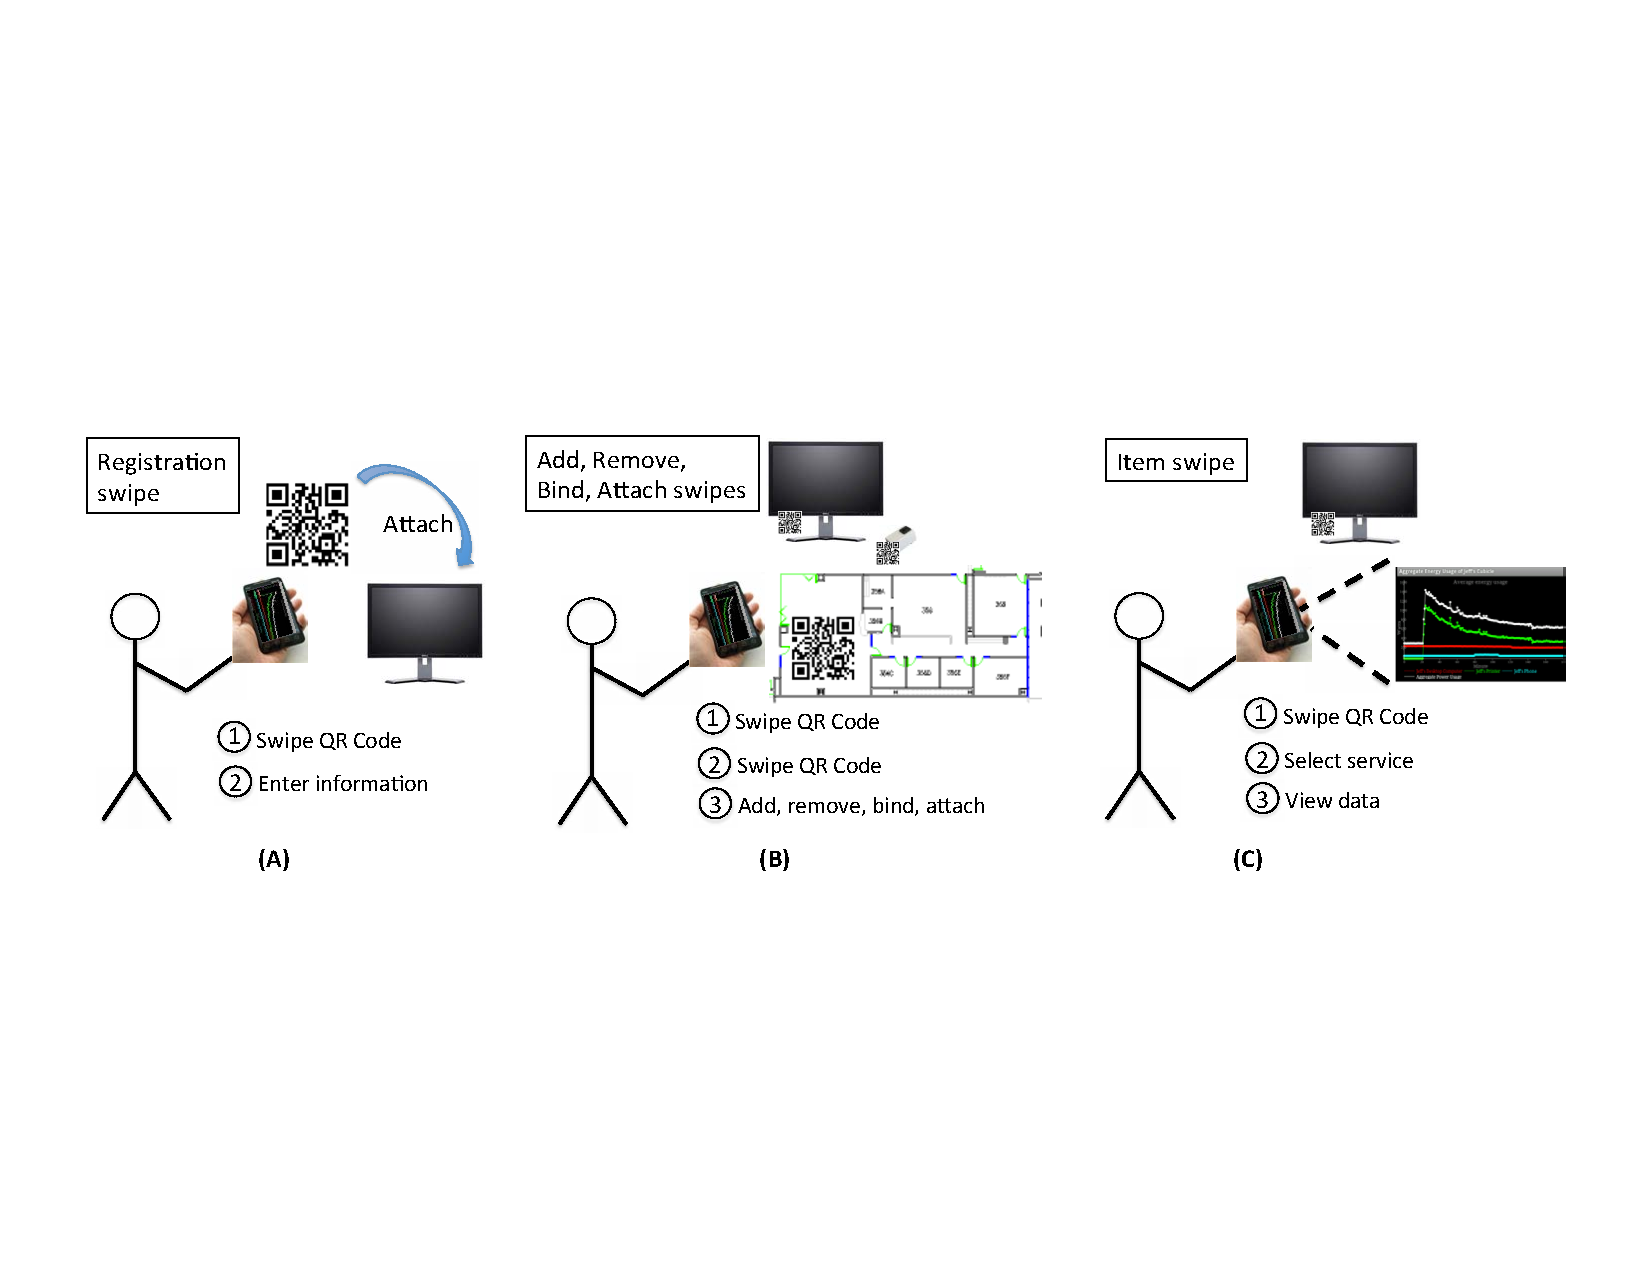
\includegraphics[width=0.8\textwidth]{figs/swipes}
\caption{Swiping gestures in the mobile application.  The registration swipe requires on a single swipe.  The 
linking and registration gestures require two swipes, and the look-up requires a single swipe.}
\label{fig:swipes}
\end{center}
\end{figure*}

The first set is called a `registration' swipe and we use it to register new items.  The user scans a QR code and the item it is atextttached
to.  This creates an `atextttached-to' link between them.  Adding, removing, binding, and atextttaching items is done with a pair of swipes.
A lookup is done with by swiping the QR code atextttached to an item.
% There are three major components in our architecture: QR codes, mobile phones, and StreamFS.

% How do we evaluate our ability to track people and things?
% This is a description evaluation.  We need to describe how the pieces interact.  What will fall out of the description is our strong dependence on occupants/users to give us information about the state of the physical world.  It’ll also fall out that what allows these pieces to fit together is network infrastructure.
We have designed a set of heuristics for setting the location during an update, that piggybacks on the swipe gesture.
The following is a list of rules for automatically setexttting the location of people and things:

\begin{itemize}
\item When a user swipes at a location L, they are presumed to be at L for fixed period $\tau$.  An ``association timer'' is set to 
        release this association after $\tau$ seconds.
\item If the user swipes anything that is associated with a location $l$ at time $t \le \tau$, and $l(t)\ne$ L, 
        then we set the new location of the \emph{thing} they swiped to l(t) and reset the association timer.
\item If the user swipes anything at location l at time $t \ge \tau$, we set the location of the \emph{person} to l(t).
        We reset the association timer to $\tau$.
\item If a user registers a new location, they are presumed to be at that location.
\end{itemize}
\vspace{0.08in}


For each of these, we provide an interactive option to ask for location-change confirmation from the user.  So if we think the
user/item has moved but they have not, the preset action can be overridden.  The guiding principal we follow in our design
is to leverage the swipe gesture for as much contextual information as possible.  Furthermore, we do not explicitly track users.
Context is only set on the phone and used in operations sent to the server.  
We then construct an entity relationship graph through 
naming in StreamFS.  StreamFS uses filesystem constructs, such as hierarchical naming and symbolic
links, which we use to express an acyclic relationship-graph structure.

 which you are either editing directly or
adding creating/destroying a relationship link in the graph.

Because location swipes give us direct confirmation of a user's location, it can be coupled with wifi localization mechanisms
and supervised learning algorithms to adjust the localization model as the user interacts with their environment. 
For future work we intend to experiment with this mechanism.% to enable supervised-learning-based indoor wifi localization.


\subsubsection{QR code design}
\label{sec:qrc}
Our choice to use QR codes is important, since the \emph{only way to scale -- in deployment size and management complexity -- is to
involve building occupants}. QR codes are cheap to produce.  They can be printed and atextttached to items with tape or sticky paper.  
Figure~\ref{fig:qrcexsecond} shows an example QR code used in our deployment.  These are placed on physical
objects and spaces throughout the building to link between the physical world and our virtual representation of it.

With the number of physical objects and places in a building, \emph{we must rely on the occupants
to scale our deployment and manage it over}. Because QR codes are easy to produce, we provide occupants with a webpage that
that produces them.  They print them out, place them on items or places they want to interact with and register them.

Since occupants are our target users, we must make the application easy to use.  For QR code usage, varied lighting conditions, 
phone-specific camera quality, and shaky hand movements can make scanning cumbersome; ultimately de-motivating continued use.  
QR codes must be designed to minimize scanning time.  In our initial deployment and experiments we observe
that complex QR code code not only have an longer average scanning time but also experience a larger variance in scanning time.  
The more complex the pixel design in the QR code, the harder it is for the camera to focus and capture it. 


We scanned each QR code shown in Figure~\ref{fig:qrcexcomp}, under light and dark lighting conditions.  
Each experiment was run 10 times and Table~\ref{tab:qrscans} shows a statistical summary.  Scanning the simple QR code under well-lit 
conditions performed the best.  The complex QR code under  the same condition takes about 28-36\% longer to scan.
Perhaps even more important is the variance.  Notice that the variance with the simple QR code is smaller.
QR code image complexity increases with the amount of information you encode on it.  Therefore, it was important to decrease the
amount of information we encoded, \emph{placing the complexity in the lookup rather than the tag.}

% \begin{figure}[htb!]
% \begin{center}
% \subfigure[Long QR Code.]{%
%             \label{fig:qrcexfirst}
%             
\includegraphics[scale=0.148]{figs/qrcexlong}
%         }
% \subfigure[Minimized QR Code.]{%
%             \label{fig:qrcexsecond}
%             
\includegraphics[scale=0.35]{figs/qrcex}
%         }
% \end{center}
% \caption{
% 	The QR code on the left resolves to the same {\texttt URL} at the right one, after resolution and
% 	redirection is complete. 
% 	The short label resolves to {\texttt htextttp://tinyurl.com/6235eyw}.  The second encodes about half
% 	the characters as the first.
% 	We used tinyUrl to reduce the QR code image complexity and scan time.
%      }%
% \label{fig:qrcexcomp}
% \end{figure}


\begin{figure}[h!]
\begin{center}

\includegraphics[scale=0.148]{figs/qrcexlong}
\caption{\ref{fig:qrcexfirst} resolves to the same {\texttt URL} as the ~\ref{fig:qrcexsecond}, after resolution and
	redirection is complete. 
	The short label resolves to {\texttt htextttp://tinyurl.com/6235eyw}.  \ref{fig:qrcexsecond} encodes about half
	the characters as the \ref{fig:qrcexfirst}.
	We used tinyUrl to reduce the QR code image complexity and scan time.}
\label{fig:qrcexfirst}
\end{center}
\end{figure}

\begin{figure}[h!]
\begin{center}

\includegraphics[scale=0.35]{figs/qrcex}
\caption{\ref{fig:qrcexfirst} resolves to the same {\texttt URL} as the ~\ref{fig:qrcexsecond}, after resolution and
	redirection is complete. 
	The short label resolves to {\texttt htextttp://tinyurl.com/6235eyw}.  \ref{fig:qrcexsecond} encodes about half
	the characters as the \ref{fig:qrcexfirst}.
	We used tinyUrl to reduce the QR code image complexity and scan time.}
 \label{fig:qrcexsecond}
\end{center}
\end{figure}

\begin{table}
\label{tab:qrscans}
\begin{center}
  \begin{tabular}{| r | c  c | }
    \hline
    			 & {\textbf Average (sec) } & {\textbf Variance (sec)} \\ \hline
    Short,light & 1.66 & 0.33 \\ \hline
    Short, dark & 2.08 & 0.35 \\ \hline
    Long, light & 2.26 & 0.71 \\ \hline
    Long, dark & 2.82 & 0.50 \\
    \hline
  \end{tabular}
\caption{Shows the time to scan a long QR code versus a short QR code in light and dark conditions (loosely defined).
Notice that short QR codes scan faster and with less variance that long ones.}
\end{center}

\end{table}

Table~\ref{tab:qrscans} shows the results of some simple scanning experiment between the two tags
shown above.  We scanned each QR code under light and dark lighting conditions, off the screen of my laptop.
Each experiment was run 10 times and the table shows the statistical
overview of the results. 
Clearly, scanning the simple QR code under well-lit conditions
performed the best.  The complex QR code under the same condition takes about 28-36\% longer to scan.
On a generic QR code scanner, as used here, there is a portion of the
scan time that is independent of the code complexity.  As these are
more heavily used, this is expected to be reduced substantially and
the difference is acquisition complexity will be even more pronounced.
Perhaps even more important is the variance.  Notice that the variance with the simple QR code is much smaller and
more stable under either condition.  In our experience, {\textbf large variance in scan time is a major
problem for complex QR codes}.  Thus we decided to re-design our codes and push more information in the lookup
processes, as network access was more reliable than the focus of the camera on various mobile devices.
Tags are placed on all types of devices in all kinds of locations with varying degrees of lighting.
Simple QR codes are vital for widespread use.

The design choice forced us to examine others that were related.  Not being able to encode much information on 
our QR codes means we are more reliant on the network to provide the bulk of the information, to be very reliable,
and to be widespread enough that disconnection is not problematic.  Moreover, there are a number of clients
that can be used to access and display the information and the tag has to be meaningful for both.
In order to meet these criteria we (1) shrunk {\texttt URL}'s using tinyURL~\cite{tinyurl} as a level of 
indirection and 
(2) designed two classes of applications: \emph{shallow} applications, and \emph{deep-inspection} applications.  Shallow
applications interact with the web-application directly while deep-inspection application use
the {\texttt URL} of the web application to extract a unique identifier and provide deeper inspection
and update capabilities of the entity-relationship graph.

This is an example {\texttt URL} we used in our deployment: {\texttt htextttp://tinyurl.com/6235eyw}.
When resolved, we get an empty response in the body, but we use the header to identify the QR code identifier 
that we associate with the item.  The response header is down in Figure~\ref{fig:tinyurlhdr}.

\begin{figure}[htb!]
\begin{center}
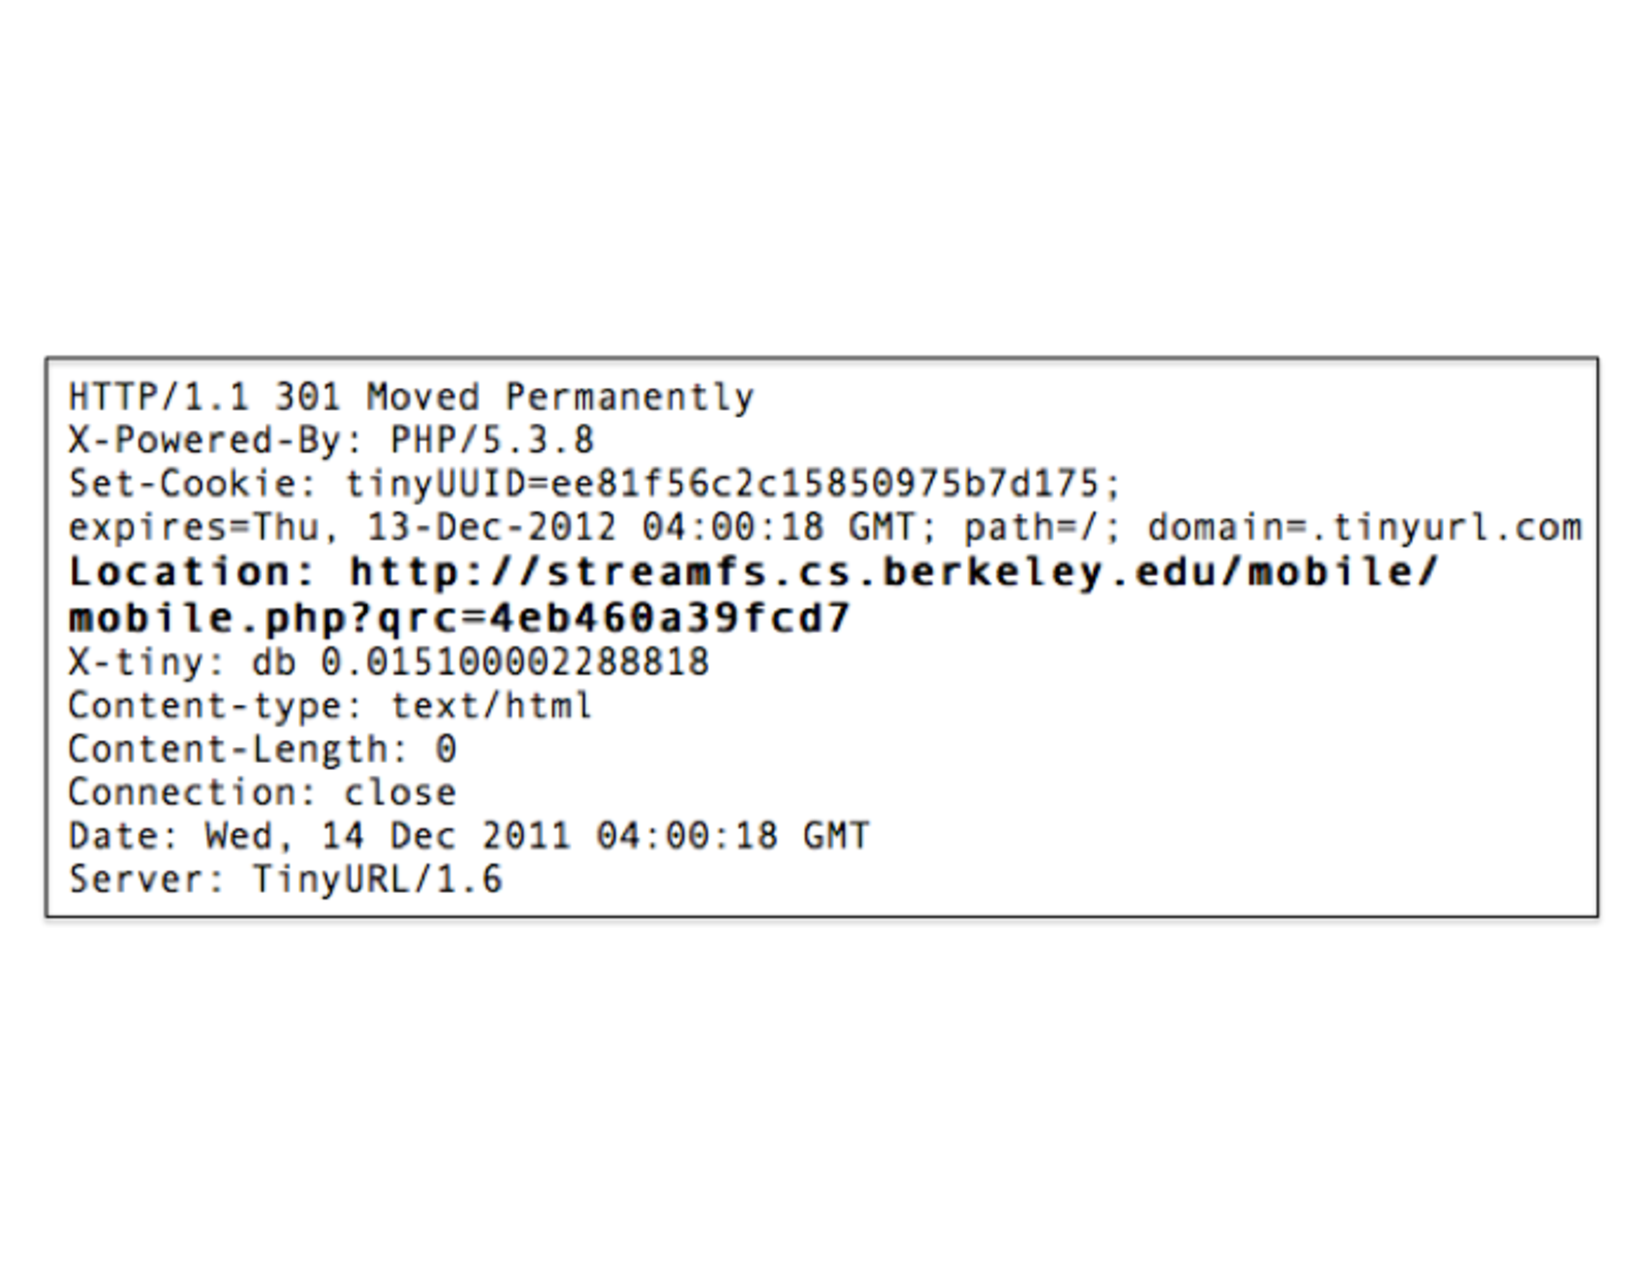
\includegraphics[scale=0.30]{figs/tinyurlhdr}
\caption{The header of the response from the {\texttt tinyUrl} when resolving a QR code.  The `Location' atextttribute
is used to extract the unique identifier for the object this QR code tags.  It is also used to re-direct
users without the phone application to a meaningful web address for the object.}
\label{fig:tinyurlhdr}
\end{center}
\end{figure}


Notice the `Location' atextttribute in the header.  This is the location of the re-direct.  This approach gives us
flexibility in several ways:

\begin{enumerate}
\item It allows us to encode less information in the QR code, decreasing its visual complexity; making it more
		robust across phones with different camera quality, poor lighting conditions, and shaky hands.
\item It allows the added layer of indirection to serve two versions of the applications:  the native application,
		where users can \emph{deeply explore} and edit the entities and their relationships and the \emph{shallow lookup}, 
		which re-directs the mobile phone to a read-only view of the item that was scanned -- such as a power trace or 
		a description.
\end{enumerate}


It provides a web address for users to re-direct to and find information and various read-only services for the object.  However, because
the {\texttt URL} also contains a unique identifier \emph{qrc}, it can be used to provide for sophisticated services and capabilities.
An example is the ability to change the virtual structure of inter-relationship between this object and other objects.  This
is demonstrated in our energy auditing application discussed in detail in section~\ref{sec:eaudit}.
Once items are tagged, they can be added and removed by swiping the tag and pressing the butexttton for what you want to do with
the item.  You also check into locations either explicit with a location-tag swipe or implicitly with an item swipe.

\emph{Shallow} applications
use the {\texttt URL} directly.  The \emph{qrc} {\texttt URL} is unqiue identifier for the item that this tag is atextttached to.
A shallow application can obtain mostly read-only service through our web applications.  For example, we'll see how
to get either item-specific data or item-aggregated data with respect to the user making the request (i.e. the total
energy consumed by \emph{my} devices).  \emph{Deep-inspection} applications are native to the phone, so we can do much
more with the tag.  Our energy auditing application allows you to related the item to other items by maintaining state of swipe
history.  This is more difficult with the web-applicaiton.  We can also use the tag and item information to couple it with
sensor information coming from sensors on the phone itself.  For example, we could determine the direction an object
is pointing by using the phone's directional sensor and negating their direction (i.e. phone is facing east, tag on item must
be facing west).

\begin{figure*}[htb!]
\begin{center}
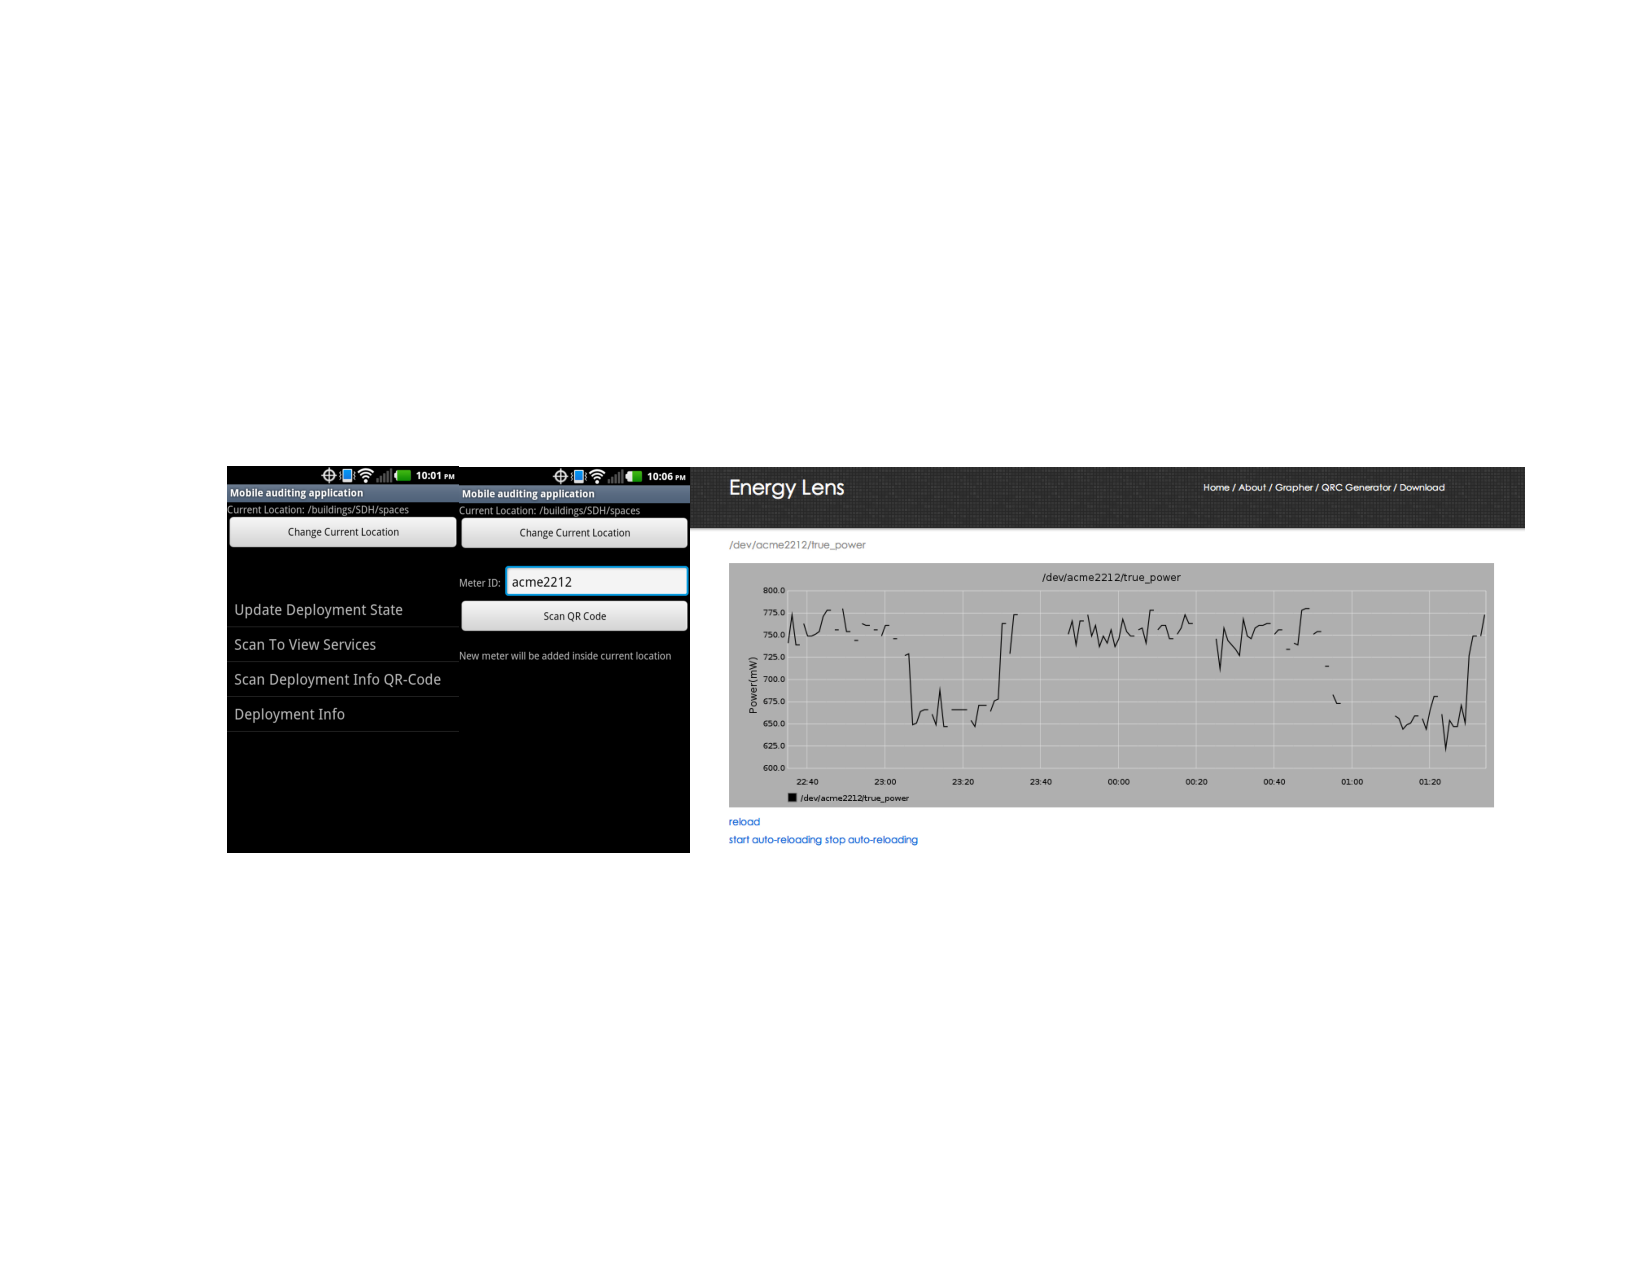
\includegraphics[width=\textwidth]{figs/mobileapp}
\caption{Screen shots of the mobile application.  The screens on the left are for editing the state of the deployment.
The graph on the right shows a live feed of a the sensor that's atextttached to the item that was scanned with the `Scan To
View Services' option in the mobile application.  It can also be resolved by scanning the QR code and following the re-direct
to the URL.}
\label{fig:mobileapp}
\end{center}
\end{figure*}

ACme meters are IP-enabled and forward their data through a router that runs sMAP.  sMAP then forwards the incoming data
to StreamFS, running in a machine in Amazon's EC2.  StreamFS is a web service that organizes streaming data and metadata using
a hierarchical naming convention.  It also provide a pub/sub facility for streaming data.  We construct 
a canonical naming convention within StreamFS to express the entity relationships between people, things, and meters.  The pub/sub
mechanism allows us to combine the ERG with streaming data, and feeds our timeseries data viewers.

\subsubsection{Entity-Relationship graph}
We construct the entity relationship graph through naming in StreamFS.  StreamFS uses filesystem constructs, such as symbolic
links and hierarchical naming which are useful for expressing an acyclic graph structure (StreamFS checks for cycles when symlinks 
are created).  
The following general path-naming text patterns are used to express different portions of the ERG.
$/path/to/device\_or\_item$, 
$/path/to/qrc$, $/path/to/space$, $/path/to/taxonomy$, $/path/to/users$.  
Registered meters are placed in the device path, {\texttt /dev}.  Items are stored in {\texttt /inventory}.  QR codes are stored 
in {\texttt /qrc}.  When an item is registered a 
symbolic link is created from the specific qr code directory to the item.  {\texttt /spaces} contains a hierarchy of floors, rooms, 
and sub-spaces.  {\texttt /users} contains the list of usernames.  We also have a {\texttt /tax} directory, where we construct an
device hierarchy for access by plug-load category.  Placement (location) is also captured with symbolic links. 

\subsection{Challenge 2: Consistency Management}
We use an eventual-consistency model for maintaining the ERG over time.  Naturally, the spatial inter-relationships
change over time as items are moved and replaced.  In order to deal with this we offer two options: 1) we periodically
re-scan the items and their locations, essentially re-capturing the inventory collection portion of the audit or
2) we allow building occupants to participate as auditors, capturing their own personal items and shared items.
This should provide at least as much value as a periodic energy audit and can be completed in a fraction of the 
time~\cite{aceee_mobileaudit}.

Placement (location) is captured with symbolic links as well.
Node types inform the application of the nature of the relationship.  We define five distinct types: item, meter, 
location, category, and tag.  The following relationships are constructed with symlinks between different node types:

\begin{itemize}
\item {\textbf Owned-by}: When a meter/item/location is tagged as belonging to a user.
\item {\textbf Bound-to}: When a meter is atextttached to an item and taking physical measurements associated with that 
		device, we say that the meter is ``bound-to'' the device.
\item {\textbf Atextttached-to}: When a meter/qr code/item is atextttached to another meter/qr code/item but \emph{not} taking any 
		physical measurements for that item, we say that the meter/item is ``attached-to'' the other meter/qr 
		code/item.  QR codes cannot not be atextttached to each other.
\item {\textbf Is-in}: When a meter/item is inside a location, we say that the meter/item ``is-in'' that location.
\item {\textbf Type-of}: When an item is labeled by as a known, specific, type, we say that the item is a ``type-of'' thing 
		specified by the its label.
\end{itemize}

All symlinks are interpreted based on these rules of association.  As items move, symlinks are removed and re-created
in a different folder.  We know your current location by following the path from the QR code directory, across a symlink, 
to a file in the space directory.  Items associated with a space have a floor or room folder point to the item
via a symlink.  This is how we record the location of things throughout the building.

\begin{figure}[htb!]
\begin{center}
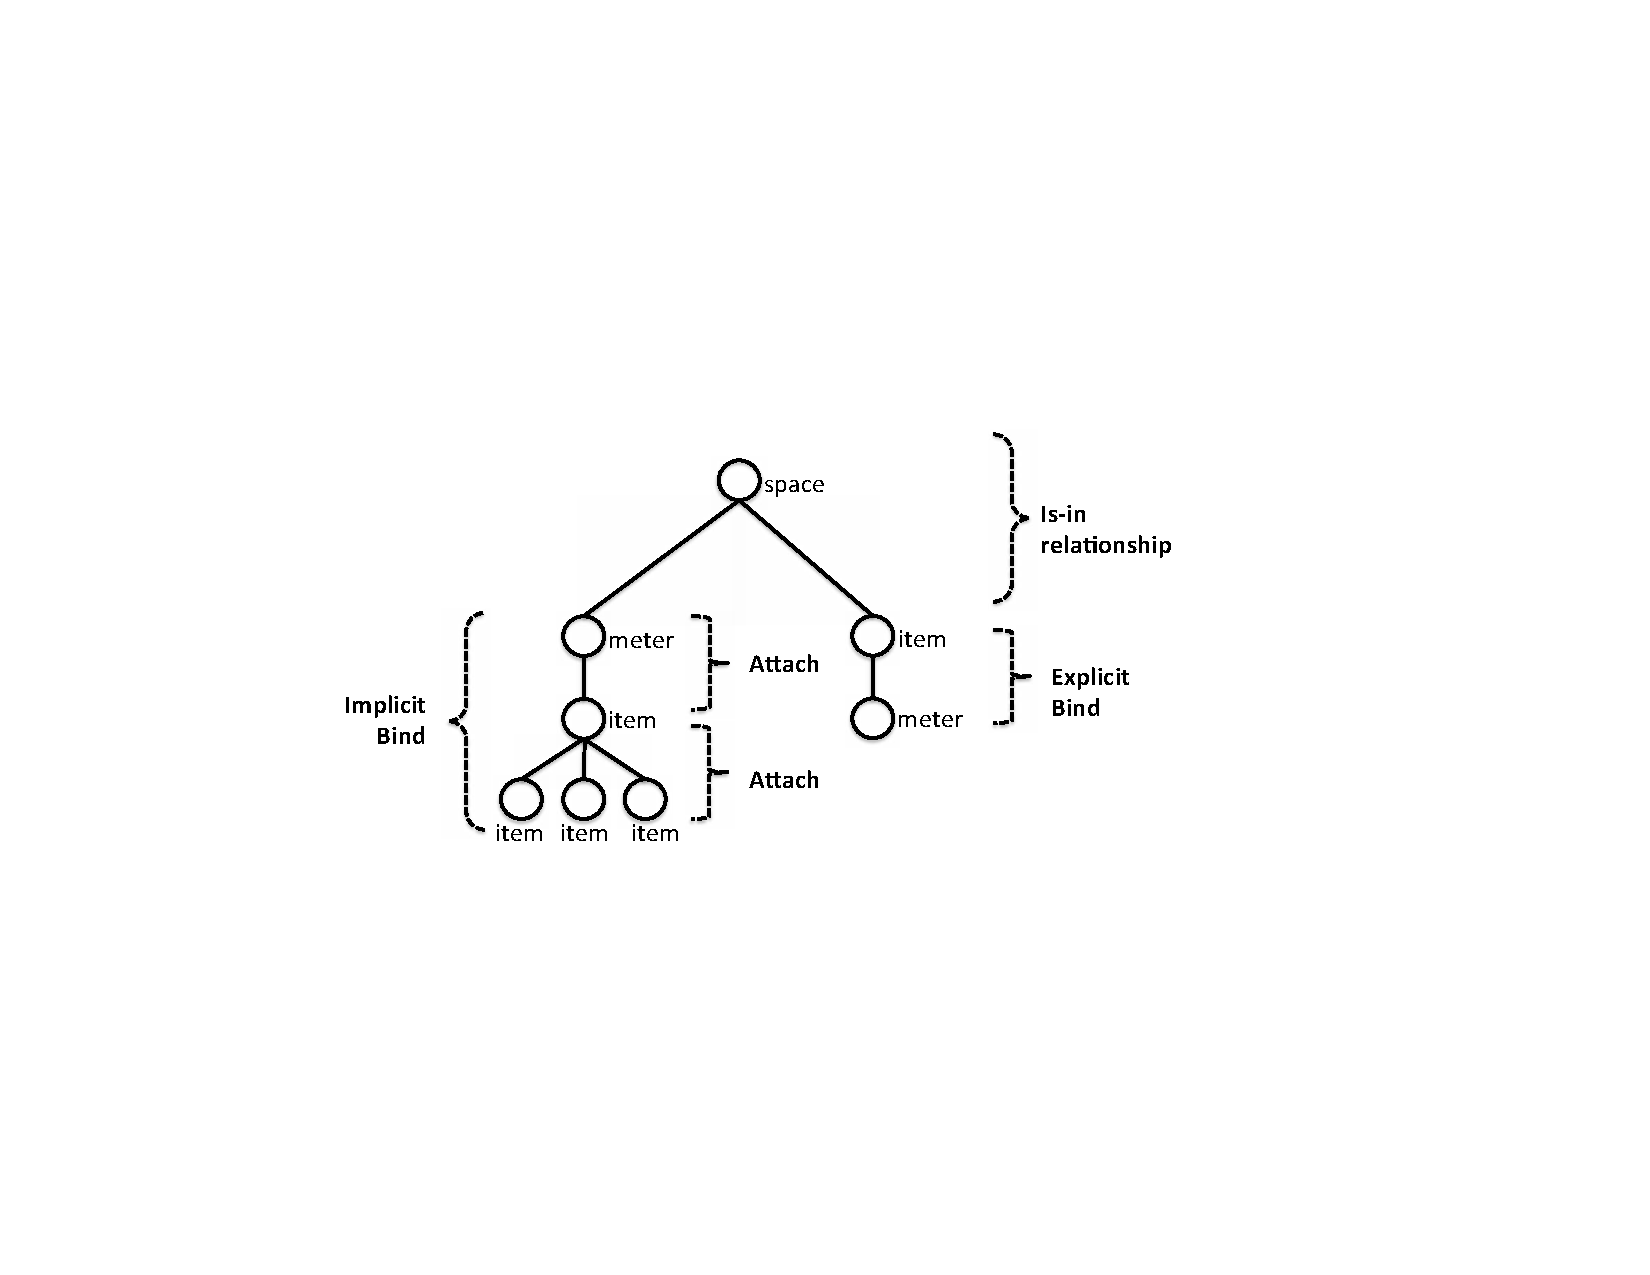
\includegraphics[scale=0.55]{figs/bindattachstructs}
\caption{This diagram shows the relationship capture between the objects and locations in the building for the 
energy audit application.  Children of a space node have an ``is-in'' relationship with the space.  An item
with another item as a child have a ``is-attached'' relationship and meters atextttached to items are bound to each other.
Note, this is a \emph{subset} of the relationship diagrams generated across our three applications.}
\label{fig:atextttachandbind}
\end{center}
\end{figure}


\subsection{Application layer}

\begin{figure}[htb!]
\begin{center}
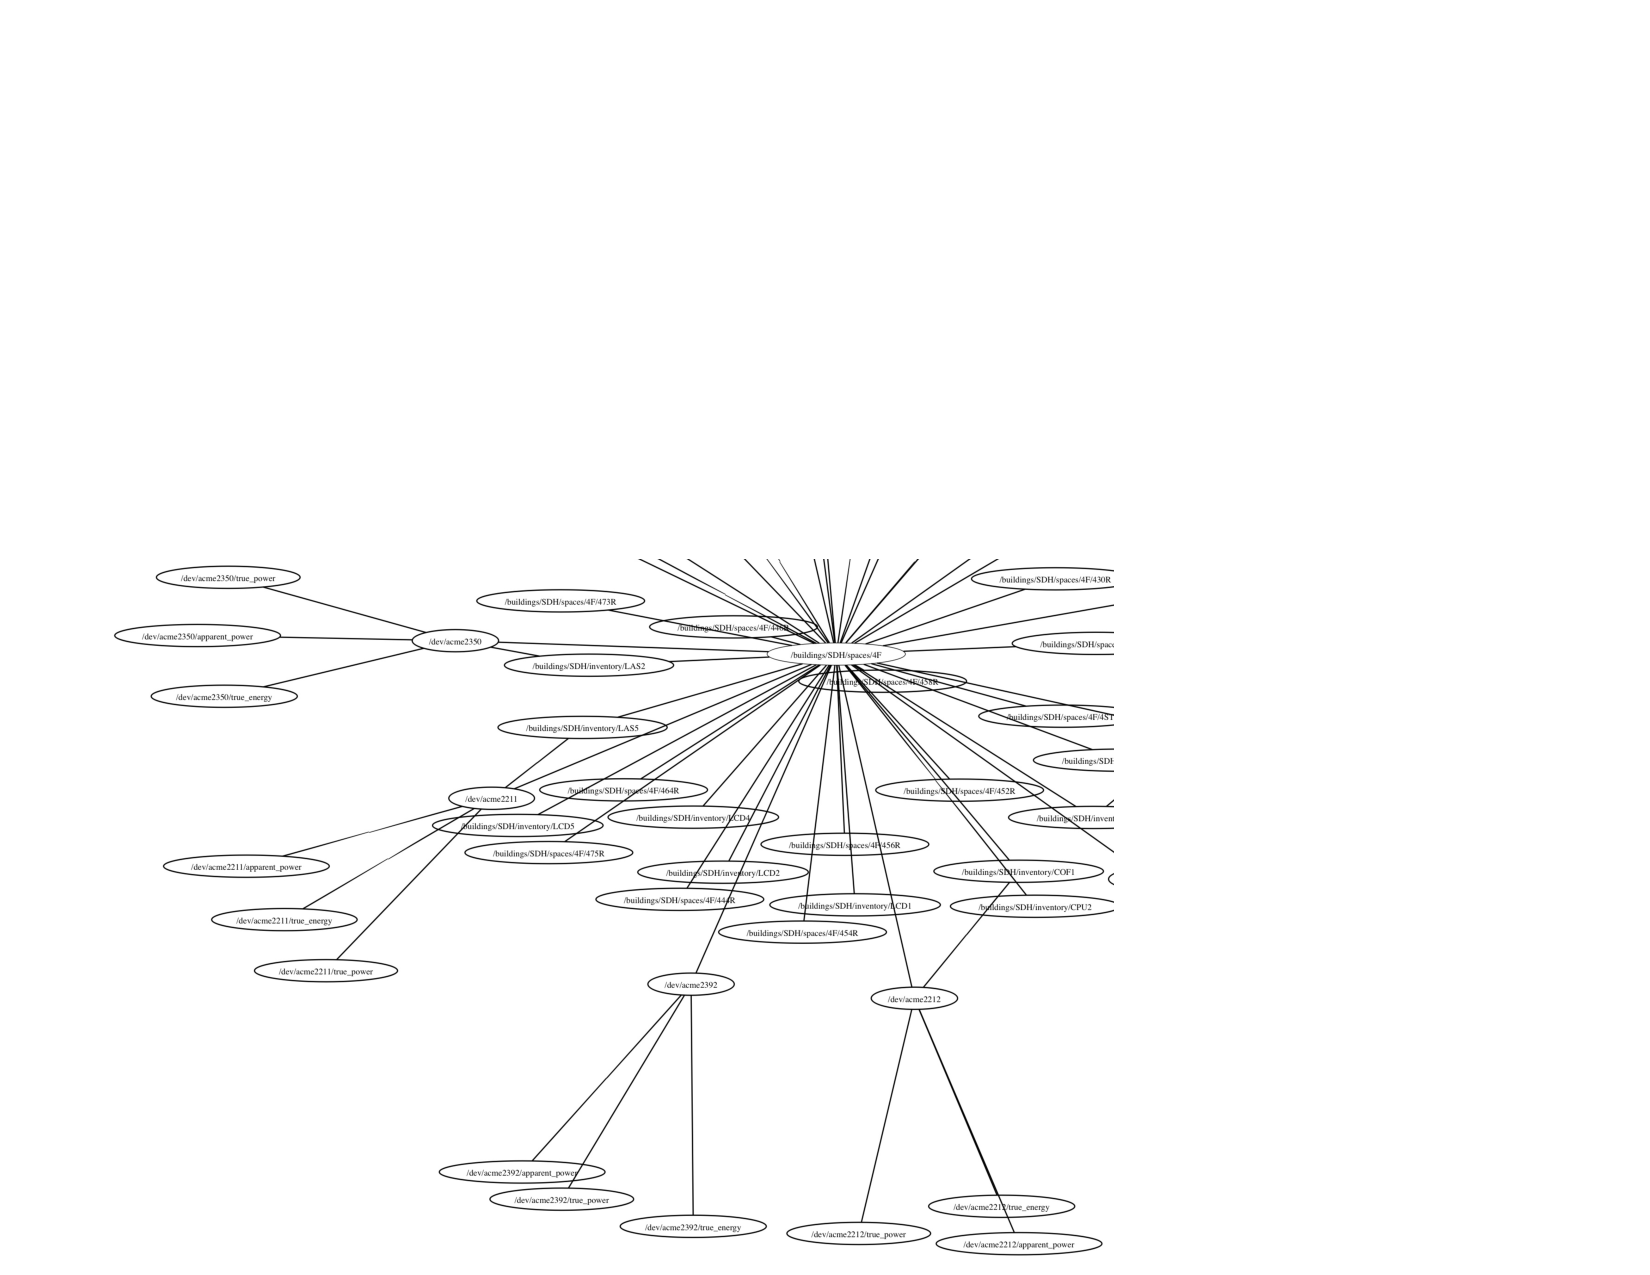
\includegraphics[scale=0.45]{figs/SDH_4F_ERG_closeup}
\caption{A portion of the prefetched entities on the a single floor in our building.  This shows a snapshot of the entity-relationship
graph for that floor.  Each node, link, and associated content is prefetched when the user swipes the floor
tag or anything on that floor.}
\label{fig:sdh_4f_erg}
\end{center}
\end{figure}




\subsection{Challenge 3: Disconnected Operation}
Although connectivity is ubiquitous, network access is not.  This occurs due to dead zones, 
idle-disconnect and failed hand-off between access points.  When encountered in practice, especially while editing
deployment state, it can be quite frustrating and discourage use of the application.  We designed a
mechanism that does smart caching, not only to improve performance, but also to allow for disconnected operation.

The Energy Lens application downloads a portion of the ERG when a user enters a new floor.  The application fetches the portion
of the graph rooted at the floor.  
Figure~\ref{fig:sdh_4f_erg} shows just a small portion of that entity-relationship graph for the floor we are monitoring in
our deployment.  
A prefetch populates the cache with all entity nodes on that floor, their associated metadata,
and 30 minutes of data from the stream entities.  The full fetch of the 4th floor data set includes
176 nodes and about 1 MB of meter data.  In total, the app downloads ~1.2 MB of data upon re-connection.
Prefetching allows users to continue interacting with the application as if they were still connected (as long as they remain on
the same floor).  Without it, the application is not functional until a network connection is established.

% \begin{algorithm}
% \caption{Prefetch Loop}
% \label{alg:prefetch}
% 	\begin{algorithmic}
% 	\While {true}
% 	\If {connected and active}
% 	    \State $req\gets [t_{i-n}, OP_R]$
% 	    \State $resp\gets $ send($req$)=$[t_{i-k}, OP_R],\dots, [t_{now}, OP_R]; $ 
% 	    \State $n >= k$
% 	    \For {$j = 1 \to size(resp)}$
% 	    	\State $op \gets$ $resp[j]=[t_{i-k+e}, OP_R]$
% 	    	\State apply($op$)
% 	    \EndFor
% 	\EndIf
% 	\If {active}
% 		\State Sleep for 10 minutes
% 	\Else
% 		\State Sleep for 1 hour
% 	\EndIf
% 	\EndWhile
% 	\end{algorithmic}
% \end{algorithm}

\begin{algorithm}[h!]
 \SetAlgoLined
  \While{1}{
	  \If{connected and active}{
	  	(1) $req\gets [t_{i-n}, OP_R]$\;
	  	(2) $resp\gets $ send($req$)=$[t_{i-k}, OP_R],\dots, [t_{now}, OP_R] $\;
	  	(3) $n >= k$\;
	  	\For{$j = 1 \to size(resp)$}{
	  		(1) $op \gets$ $resp[j]=[t_{i-k+e}, OP_R]$\;
	  		(2) apply($op$)\;
		}
	  }

	  \If {active}{
		(1) Sleep for 10 minutes\;
	 \Else{
		(1) Sleep for 1 hour}\;
	}
  }
 \caption{Prefetch Loop.}
 \label{alg:prefetch}
\end{algorithm}


The Energy Lens periodically syncs with StreamFS to obtain updates to the ERG and maintain a locally consistent view.  
Let $OP_R$ be an operation performed on the node rooted at node $R$ and $t_i$ be the current time on the phone.  
% Algorithm~\ref{alg:prefetch} shows the pseudo code for the prefetch process.  
After a set period, the phone sends the server
its last performed operation and the time that operation was performed.  The server responds with any operations that have
take place since then.  The client applies those operations internally to the cached version of the the ERG in order to 
maintain consistency.  The ``\emph{active}'' parameter-check, is for energy savings.  If the phone application is active, the
check occurs every 10 minutes, otherwise it occurs ever hour.

The process is demonstrated in Figure~\ref{fig:interactions}.  The components shown are the \emph{ERG cache}, the \emph{operation
log (OpLog)}, and the \emph{prefetcher}.  We separate the steps in the figure as a READ sequence and a WRITE sequence.
All reads go to the cache (steps 1 and 2 on the left hand side of the figure).  Writes go through the OpLog (steps 1 - 5 on the right
side of the figure).  For writes, 
the application makes a write request (1) and it is forwarded to StreamFS (2).  If StreamFS is reachable and the write is
successful (3), the operation is applied to the ERG cache (4) and the response is sent the application (5).
If the operation is not successfuly, step 4 is skipped.  If StreamFS could not be reached, step 3 is skipped, and the operation
is writexttten to the OpLog.  The OpLog is flushed to the server, by the prefetcher, upon re-connection. 

The OpLog contains records of operations that are eventually applied to StreamFS.  Some of those operations
are actually groups of operations that need to be applied atomically.  For example, 
when a bind or atextttach operation occurs, we append the timestamp to the item(s) that are being connected, as well as create
a link between them in the graph.  The application uses both the link and the added metadata to fetch the appropriate
graph for display.  These operations must be applied atomically or not be applied at all.
When the log is dumped, the global transaction manager (GTXM) -- the layer that handles log dumps and transaction processing --
atextttempts to apply the log in timestamp order.


\begin{figure}[htb!]
\begin{center}
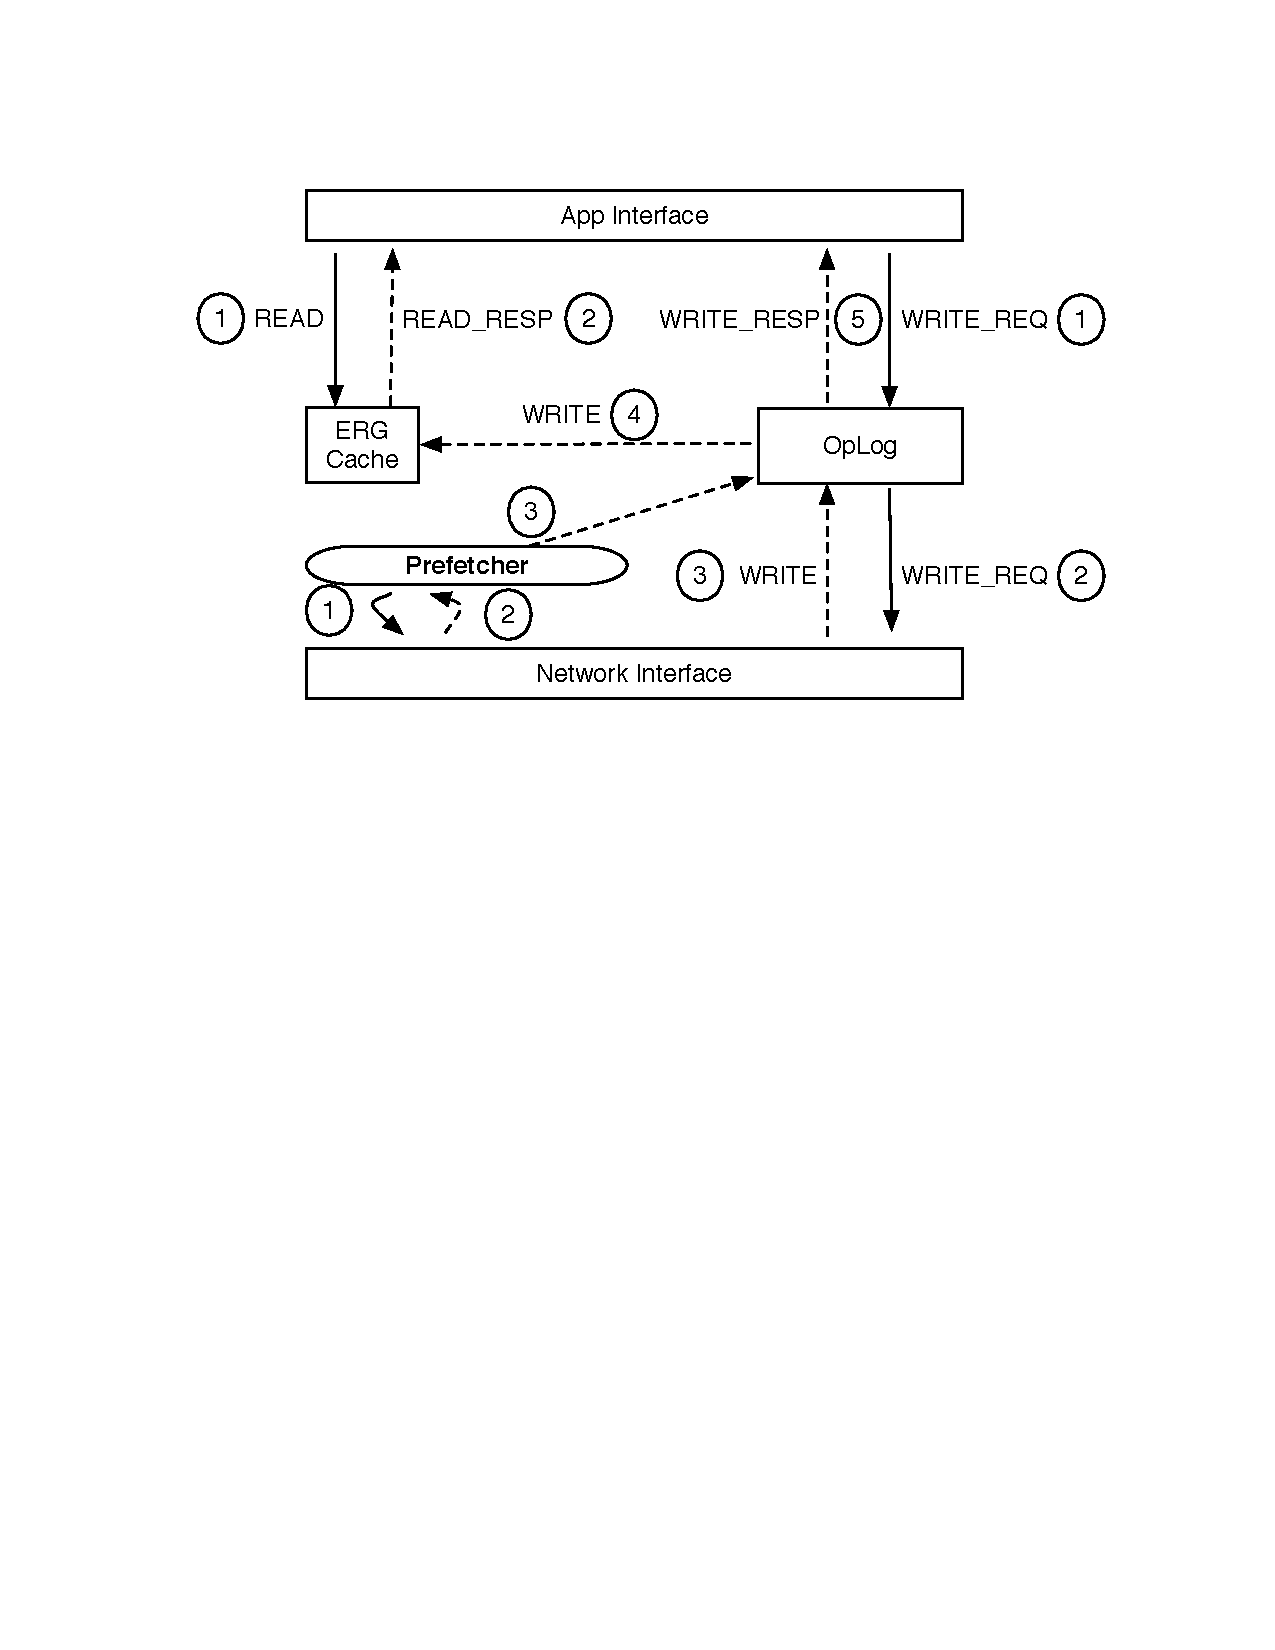
\includegraphics[scale=0.50]{figs/standard_interaction}
\caption{Standard mechanisms for consistency management on the phone.  All READ request go to the local
cached version of the ERG.  All WRITES must go through the OpLog.
They are eventually applied to the cache
if successful and logged if the StreamFS is unreachable.}
\label{fig:interactions}
\end{center}
\end{figure}

\subsubsection{Log dumps and conflict resolution}
\label{sec:conflicts}
When the Energy Lens application is started it contacts the server and atextttains the server's local clock time. 
It notes its local time as being equal to the timestamp of the server and calculates all subsequent timestamps
using its local clock.  When an operation or transaction is added to the OpLog, a timestamp is appended.  Let $t_s$ be the timestamp 
on the server, $t_l$ be the timestamp on the phone when $t_s$ is recorded, and $t_{now}$ be the current time on the phone.  
Each operation/transaction is timestamped with $t_{approx}$ where:

\begin{equation}
t_{approx} = t_s + (t_{now} - t_l)
\end{equation}

This timestamp is a general approximation of when the operation should be applied on the server.  The server applies 
these is ascending timestamp order.

Generally, a conflict occurs if there is any operation or transaction that was applied after the timestamp of the current operation
being processed.  A typical transaction manager must rollback the state of the database, apply the operation, and replay
the log.  However, conflict resolution is much simpler in this context.  \emph{The latest operations reflect the state of the
world because they are updates induced by direct interaction with the world at that point in time.}  Therefore, if there is a conflict
between a set of operations, the old ones can all be discarded.

Operations that are discarded are done so silently.  We make failures silent for two reasons: 1) There is no way to contact the app when 
failure occurs.  Mobile phones
do not often have reversably reachable addresses.  2) Failure assumes the operation was based on a false assumption about the state
of the world.  



\subsection{Real-time analytics}

Figure~\ref{fig:tsdata} shows three screen shots of power traces obtained from the ACme deployment, and displayed
through the Energy Lens.  Notice that there is
some data missing in the graph.  This occurs because of in the network transmission, reboots on the data management layer,
or failed scripts that are automatically restarted.  In all cases we get holes in the data.  To compute aggregates, interpolation 
is necessary.  StreamFS offers a real-time processing facility, whereby javascript operaters can be applied
to streaming data.  This allows us to clean it as it comes in and compute the aggregate traces.  We are currently experimenting
with various aggregation models to give occupants deeper insights.  


\subsection{Deployment Experience}
\label{sec:eval}

We deployed 20 ACme power meters~\cite{acme} on a single floor of a building on campus.  The data was made available through
sMAP~\cite{smap} and forwarded to our processing and data management layer, StreamFS~\cite{streamfs}.  We distributed
the ACmes throughout a single floor in our building and registered various plug loads as being measured by them.  We also tagged
hundreds of items and locations throughout the entire building.  In total we tagged 20 meters, 20 metered items, 351 un-metered items,
 and 139 rooms over 7 floors.  Figure~\ref{fig:tsdata} shows three screen shots of power traces obtained from the ACme deployment, and displayed
 through the Energy Lens. 

\begin{figure}[htb!]
\begin{center}
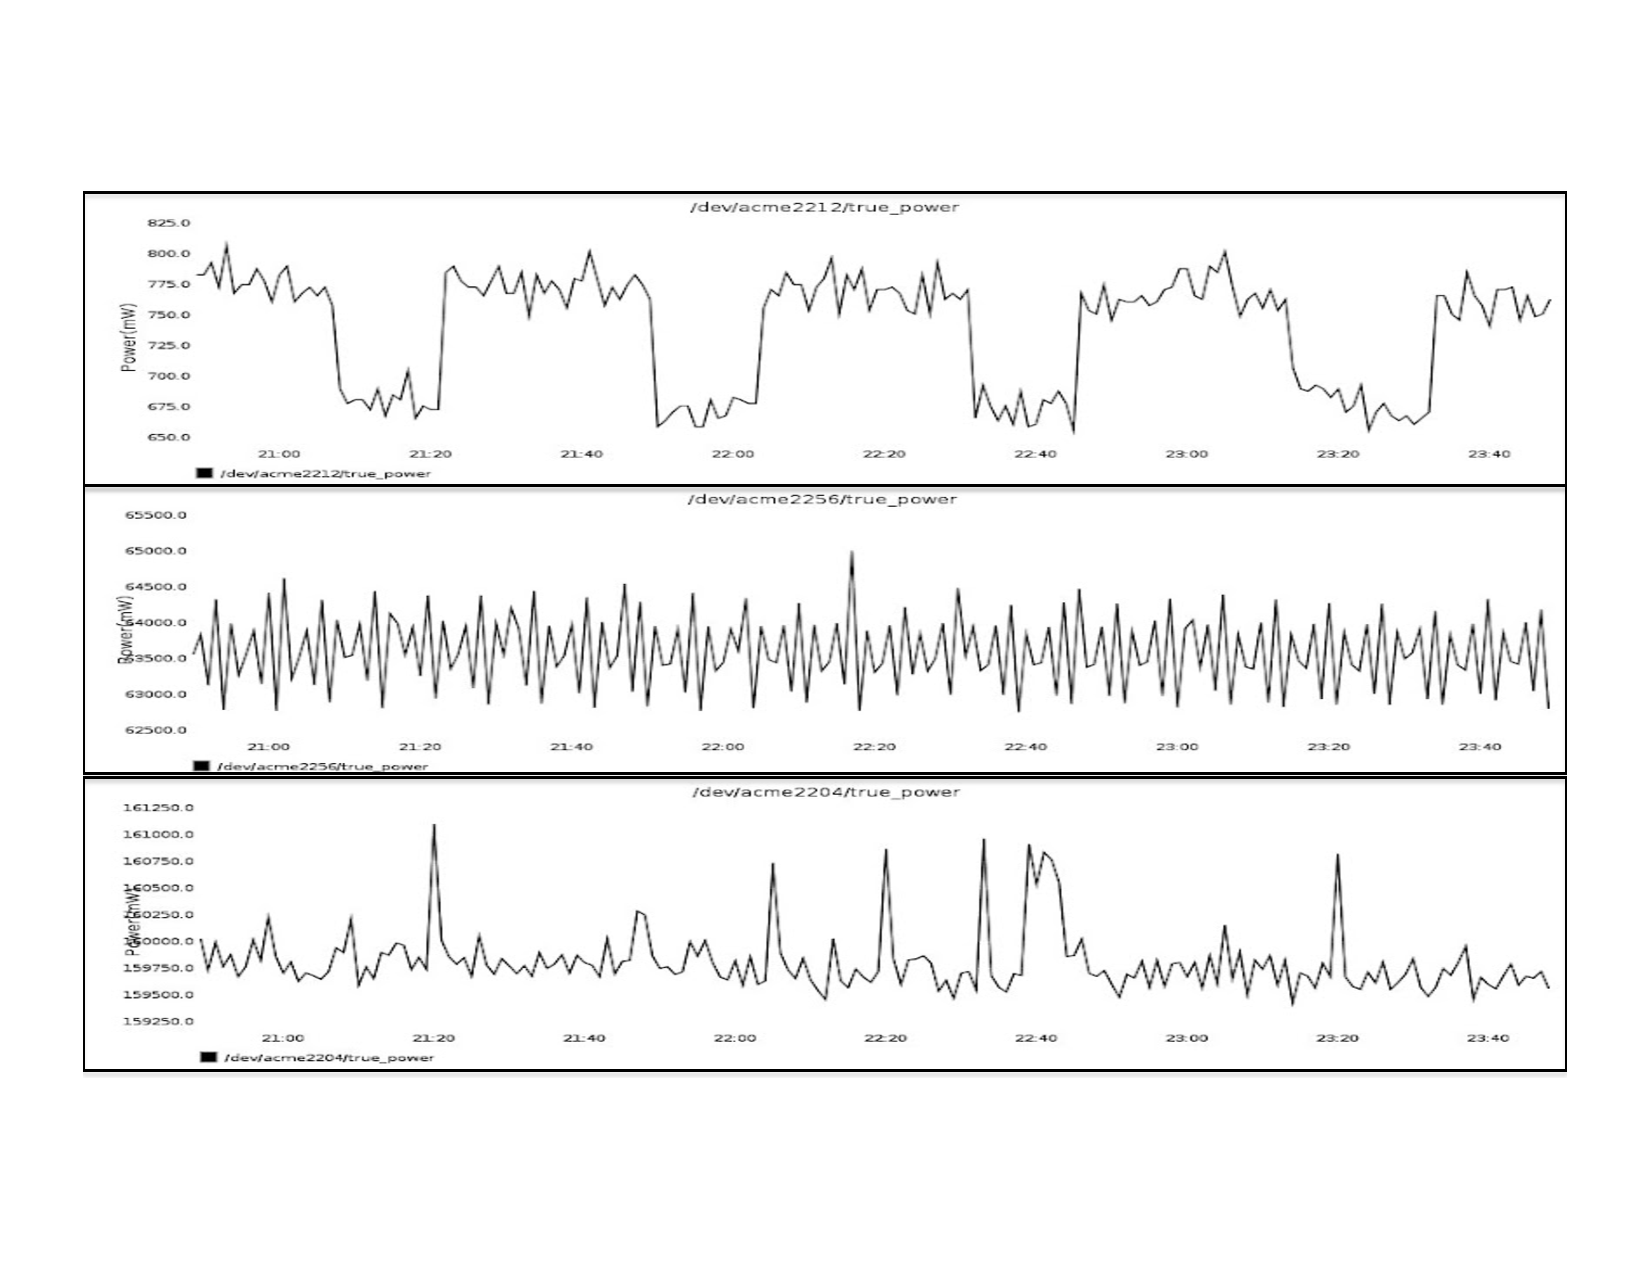
\includegraphics[scale=0.33]{figs/graphs_screen}
\caption{Power traces obtained from power meters atextttached to various plug load on one of the floors of
a building on campus.  These show screen shots of the Energy Lens timerseries data display.}
\label{fig:tsdata}
\end{center}
\end{figure}

In our initial deployment we found that the use of our tracking scheme to be effective, especially in conjunction with
interactive confirmation.  The ERG was effective at capturing deployment state, although highly mobile items, such as laptops,
were particularly difficult to keep track of.  Finally, our disconnected operation mechanism was effective at masking 
intermitextttent connectivity.  For future work we will baseline the floor's energy consumption before and after the deployment 
and measure if more visibility and analytics indeed motivates occupants to use less.

% \section{Acknowledgements}
% This work is support by the LoCal NSF Grant \#CPS-0932209 and ActionWebs NSF Grant \#CPS-0931843.  We would also like
% to thank Albert Goto for deployment help and Amazon for providing our computing infrastructure.

% Pub/sub architecture
% time decoupling
% variable time-decoupling achieved through the datastore as a buffer
% synchronization decoupling
% Either the publisher or subscriber run asynchronously.
% space decoupling
% The subscriber doesn’t have an explicit reference to the publisher.
% Programming model for real-time data
% Naming/tagging streams
% Dealing with dynamism through tagging
% Built-in functions for physical data
% heat modeling
% electrical modeling
% mathematical modeling

% Security and privacy
% Discussion.  Various topics related to StreamFS here.  Also some topics related to managing security in StreamFS for doing control.  Include another half page, perhaps.


% * Experiment that we need to run.\\
% ** Code that needs to be writexttten and experiment that needs to be run


\section{EnergyLens Evaluation}
\label{sec:eval}


In this section we measure prefetch download times and discuss strategies for providing scalability.  We also
look at the transaction manager and discuss conflict resolution.

\begin{figure}[htb!]
\begin{center}
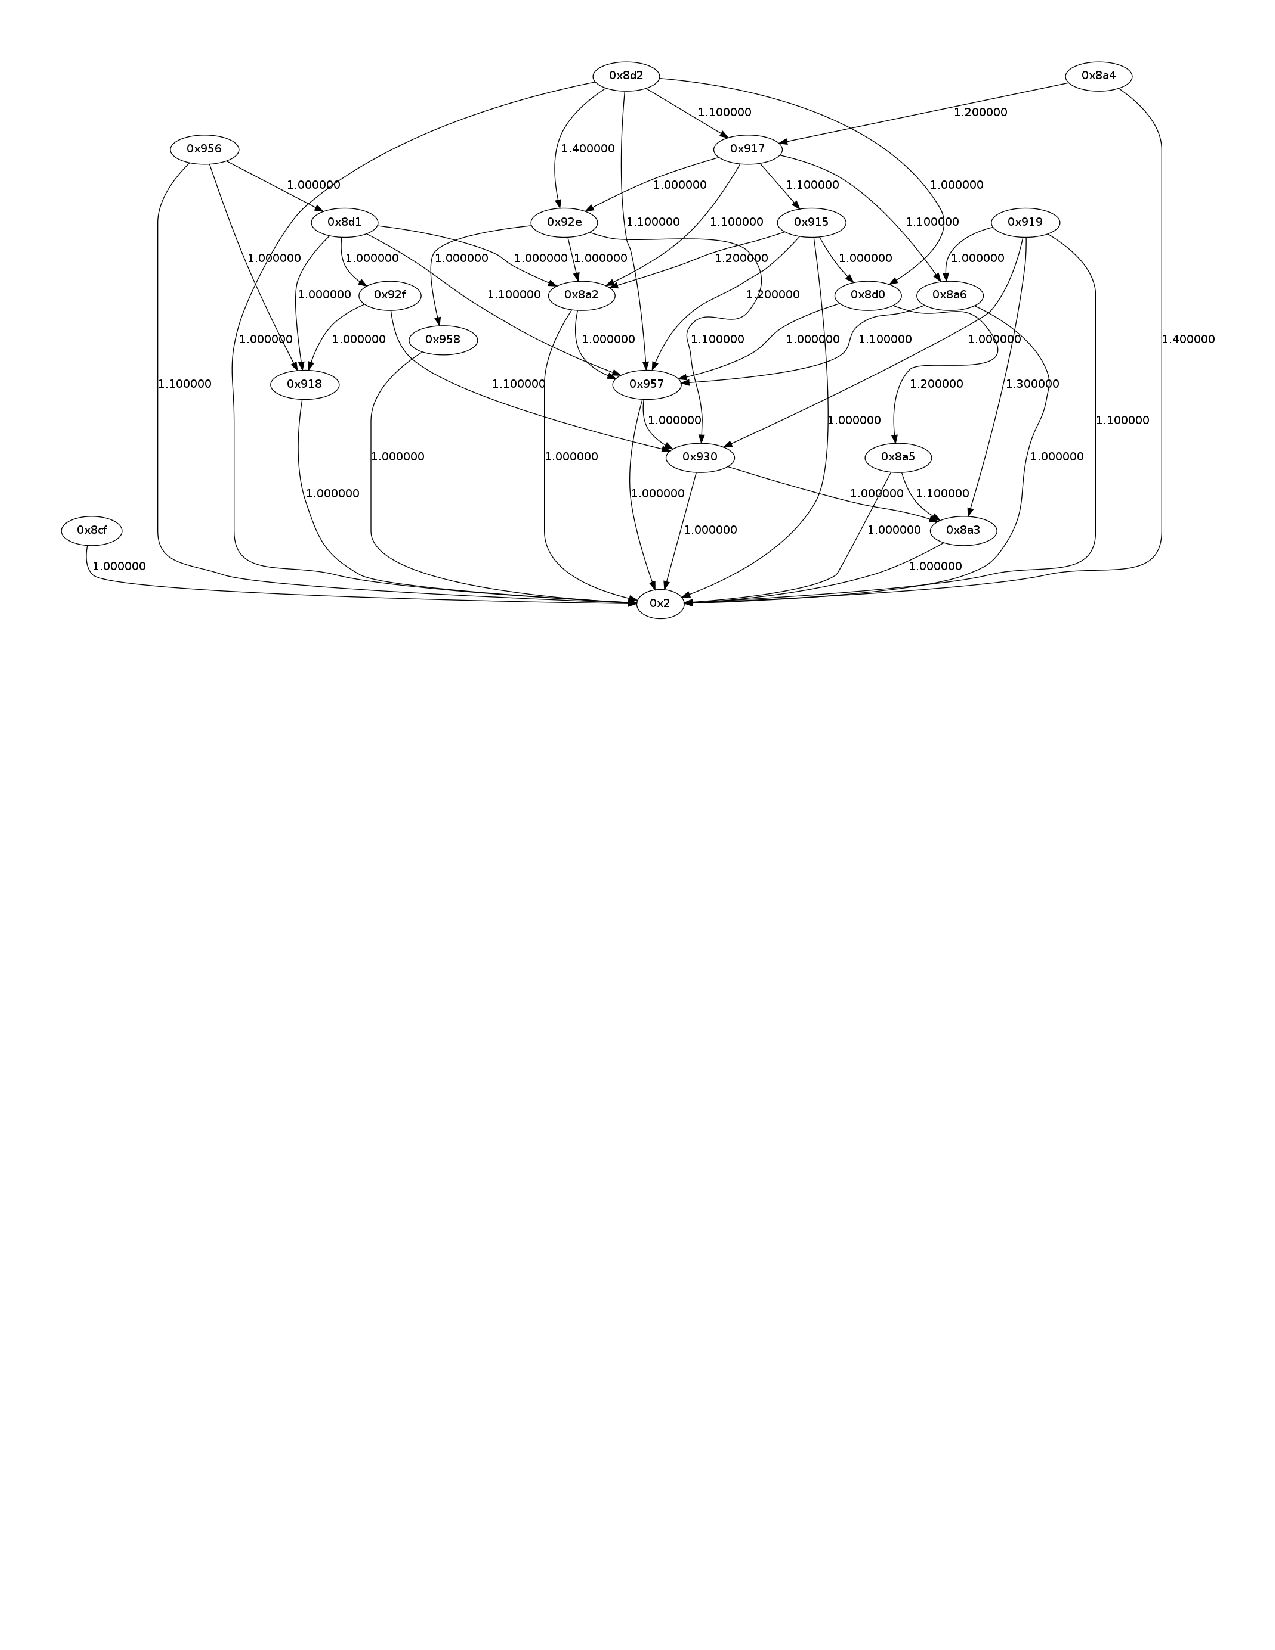
\includegraphics[scale=0.4]{figs/acmenetwork_SDH_4F}
\caption{}
\label{fig:acmenetwork_SDH_4F}
\end{center}
\end{figure}
\subsubsection{Sensing and tag layer}
We deployed 20 ACme power meters~\cite{acme} on a single floor of a building on campus.  The data was made available through
sMAP~\cite{smap} and forwarded to our processing and data management layer, StreamFS~\cite{streamfs}.  We distributed
the ACmes throughout a single floor in our building and registered various plug loads as being measured by them.  We also tagged
hundreds of items and locations throughout the entire building.  In total we tagged 20 meters, 20 metered items, 351 un-metered items,
 and 139 rooms over 7 floors.

\subsubsection{Prefetching}
Prefetching occurs when a user enters a new floor, as detected by a floor scan or an item
scan.  Table~\ref{tab:prefetchtimes} shows that the prefetch times scale linearly with the number of
items (and data) to prefetch.  Each node holds approximate 100 bytes or information and for
a 20-node deployment of power meters, producing 100 bytes of data per stream (three streams per ACme) every 20 seconds, we fetch 
approximately 1 MB of data.

These prefetch times are non-trivial to deal with, especially since they cause the phone application to slow down
until the data is received and loaded into the local cache.  The overhead is dominated by the query in StreamFS that 
constructs the entire sub graph to send to the application.  For future work,  we are will implement a
callback facility and pass the application a reference to it.  The app can then periodically check back until
the query completes and the data is ready to be downloaded.  We can also include partial responses to the query
in the prefetch-loop response.  This also allows users to continue using the application without any frustrating waits.

\subsection{Log dump measurements}
\begin{table}
\begin{center}
  \begin{tabular}{| r | c  c | }
    \hline
    {\textbf No. nodes } & {\textbf Fetch time (sec) } & {\textbf Std. Error (sec)} \\ \hline
    1 & 0.8902 & 0.0756 \\ \hline
    10 & 5.7342 & 1.7087 \\ \hline
    100 & 52.3145 & 14.1146 \\ 
    \hline
  \end{tabular}
\caption{Shows the time to fetch nodes based on the size of the fetch.  The fetch time
increased linearly with the number of nodes.  Caching maintain fetch time near
that of fetching a single node.  A callback is used when cache is invalidated.}
\label{tab:prefetchtimes}
\end{center}
\end{table}


\subsubsection{Log replay latency}
Table~\ref{tab:optimes} shows the  operations that the transaction manager calls on the StreamFS server.
Log replay and transaction processing is entirely dependent on the time to execute these operations on StreamFS.
There are five types of transactions, a \emph{move}, a \emph{un/bind}, \emph{un/attach}.  A move is a combination
of a `delete' and a `create link', a bind is a `create link' and an `update tags', an unbind and unattach is a
`delete' and `update tag'.  The transaction latency is the sum of these operations.  By far the most expensive
operation is a `create node' operation.  This occurs when a user adds a new item/space/person to the graph.
The time to apply the operation also scales linearly with the size of the logs.  

All logs dumps are processed sequentially.  However, for future work we look to parallelize processing into
parallel processes updating different portions of the graph.  For example, log updates rooted at different floors
could occur simultaneously.

The global transaction manager implements three main high-level operations -- rollback, apply, and replay.  Our current implementation
is limited by the time is takes to perform an operation on StreamFS.  Table~\ref{tab:optimes} shows the three 
main operation that the transaction manager needs to do on the server.
% Maybe we include another table that talks about the trace we ran through and the conflict times, etc.

Usually rollbacks consist of \emph{delete} operation and applies consist of \emph{creates}.  In a worst-cases analysis
of performance we expect the total conflict resolution time to be roughly bounded by
$rollback\_time + apply\_time + replay\_time$, since $replay\_time=3 X rollback\_time$ and apply\_time is negligible, 
the total time is approximately $4 X rollback\_time$.  Therefore the overhead is driven by how many new links were created
that have to be deleted and then re-created.  As an optimization, we limit the scope of a rollback.  The naive
approach is to blindly undo all operations up to a certain time.  However, we can use the location of the node
in the ERG to limit the conflict-scope to a sub graph, rather than the entire graph.  The simplest approach is to check if the operation
on a node either shares an immediate parent with the node that will have an operation undone on it or it the operation
is on the same node.  By limiting conflict-scope we minimize the number of operation that get execute and, hence, minimize the 
cost of resolution.



\begin{table}
\begin{center}
  \begin{tabular}{| l | c  c | }
    \hline
    {\textbf Operation } & {\textbf Avg. exec. time (ms) } &\\ \hline
    fetch & 250 &\\ \hline
    delete & 326  &\\ \hline
    update tags & 267  &\\ \hline
    create link & 250  &\\ \hline
    create node & 1036  &\\ 
    \hline
  \end{tabular}
\caption{Average operation execution time in StreamFS.}
\label{tab:optimes}
\end{center}
\end{table}

% \begin{itemize}
% \item Forwarding
% \item Conflict resolution
% \end{itemize}




% The main driver for the EnergyLens work is to explore the fundamental challenges related to:

% \begin{enumerate}
% \item Tracking people and objects.
% 	\begin{itemize}
% 	\item Through local crowd-sourcing of the tasks to building occupants
% 	\end{itemize}
% \item Maintaining consistency between the relationship between physical items and the entity-relationship graph that represents it.
% \item Providing real-time statistics, information, and processing of energy data related to the building environment.

% 	\begin{itemize}
% 	\item With respect to the occupants
% 	\item with respect to spaces
% 	\item Maintaining security and privacy
% 		\begin{itemize}
% 		\item specifically with respect to personal data and control
% 		\end{itemize}
% 	\end{itemize}

% \end{enumerate}







\section{Related work}

%\begin{itemize}
% \item dashboard
% \item andrew's lightin control work
% \item Kamin's hvac control work
% \item BEMs
% \item sMAP stuff
%\item Buildsys 2010 work~\cite{hbci}
%\item distributed consistency management: COPS
%\item mobility: tracking things with RFID~\cite{rfid_gonz2006}
%\item mobility: tracking of people, wifi indoor localization
%\item entity-relationship graphs
%\item homeOS [microsoft]
%\item HP Cooltown~\cite{cooltown}
%\end{itemize}
Our work touches on several areas from smart home research to logistics.  In the building space, there has been
some interest in building various kinds of energy-related visual and control applications.
This work focuses on the object definition, tracking, and management component of the architecture proposed by 
Hsu et al.~\cite{hbci}.  Their work stratefied the set of challenges that one could potentially face if the application 
were deployed at scale.  Our
work, in constrast, bases its design rationale on a \emph{real deployment} that is taking place at scale in a building 
on our campus.  We focus on solving fundamental systems challenges in dealing with intermittent connectivity
and conflict resolution in tracking people and things over time.  We also focus on leveraging gestures to minimize
the cost of interaction for users, while maximizing the information we can attain about the state of the world.

% Tracking people/indoor localization
An important aspect of the Energy Lens is determining when people and things have moved.  This requires some form 
of indoor localization.  There's a large body of literature in the area of indoor localization with mobile phones ranging from 
using wifi~\cite{radar}, to sonar~\cite{cricket}, to ambient noise~\cite{abs}, and a combination of sensors on the 
phone~\cite{surroundsense, darwinphone}.  Dita~\cite{dita} uses acoustic localization of mobile phones and also uses the infrastructure 
to determine gestures in free-space that are classified into pre-defined control actions.  Each of these require relatively complex 
software and/or infrastrure.  
We take a radically different, simple approach.  We use cheap, easy to re/produce tags (QR codes), place them on things in the 
environment over incrementally and use the natural \emph{swiping gesture} that users make, when interacting with the Energy Lens 
application, to track when they have moved or when the objects around them have moved.  The working principal is to attain as much 
information from their gesture to determine when something/one has moved.  We discuss our heuristics in section~\ref{sec:swipes}.

% context-aware apps
ACE~\cite{ACE} uses various sensors on the phone to infer a user's context.  The context domain consists of a set of user activities
and semantic locations.  For example, if ACE can distinguish between {\tt Running, Driving, AtHome, or InOffice}.  ACE also infers 
the one from the others, so if the user is {\tt AtHome} then they are not {\tt InOffice}.  Energy Lens uses inference to determine
when a person or thing has moved.  Certain swipe combinations give us information about whether they moved and where they moved to or
whether an item moved and where it moved to.  The main difference is that we only infer context when a user is actively swiping, rather
than a continuous approach.  Pretching is a fundamental technique used in many domains.  However, the cost of a prefetch for mobile
application outways the benefits if the prefetched data is not useful.  Informed mobile pretching~\cite{IMP} uses cost-benefit analysis 
to determine when to prefetch content for the user.  In the Energy Lens context, we prefetch data based on their location swipes.
We also rely on pretching to anticipate loss of connectivity, not just to improve preformance.

% Tracking things
Logistic systems focus on the tracking of objects as the move through distribution sites to warehouses, stores, shelves,
and purchase.  Items are tracked through bar code or RFID readers.  However, the workload is very structured and well
defined.  The authors of~\cite{rfid_gonz2006} describe this structure and leverage it to minimize storage
requirements and optimize query-processing performance.  Energy Lens uses the QR codes as the tag and the phone as an active
reader.  As objects move, users scan those items to their new location.  However, objects may belong to one or
many people, they can be metered by multiple meters a day, and their history in the system
is on-going.  In contrast, a typical logistics workload has a start (distribution site) and end point (leaving the store
after a sale).  In our workload, relationship semantics are important; we need to know whether the meter is \emph{bound-to}
rather than simple \emph{attached-to} an item.  We discuss the difference later in the paper.
% In addition to traditional logistics-style queries -- \emph{What is the average time that it took coffee-makers to move from the 
% warehouse to the shelf and finally to the checkout counter in January of 2004?} -- energy-analytics requires queries to group
% partial traces from meter data by tracking what meters the item attached to over the specified time-frame.
% The Energy Lens system collects and manages this kind of information to enable such queries.
Furthermore, we take advatange of natural gestures the user makes with the phone while scanning QR codes to extract
information about the current location of the user or things.

% Tagging items, virtual services
The key idea in the HP Cooltown~\cite{bridgingphysical,cooltown} work is to web-enable `things' in the world, grouped-by
`place', and accessed by `people' via a standardized acquisition protocol (HTTP) and format (HTML, XML).  
Cooltown creates a web presence for things in the world either directly (embedded web server) or indirectly 
(URL-lookup tag) as a web page page that display the services it provides.  Many of the core concepts in Cooltown 
also show up in Energy Lens.  The main overlap is the use of tags in the world that contain a reference to a virtual 
resource, accessible via HTTP through
a network connection.  Cooltown, however, explicitly chooses not maintain a centralized relationship
graph, it leverages the decentralized, linking structure of the web to group associated web pages together.
Furthermore, things are assumed to not move.  People are the main mobile entities.  The kind of applications
we wish to support must track where things are and their specific inter-relationships.  We imposed a richer set of 
semantics on our, centrally maintained, relationship graph and use it to provide detailed energy information.


\section{Summary}

% StreamFS consists of over 20,000 lines of code and was implemented in mostly Java.  It was deployed across multiple
% buildings and several applications were built on top of it over a 2 years period.

In this chapter we gave an overview of the main components in StreamFS.  Each of the components addresses the concerns stated in 
section~\ref{sec:shortcomings}.  The filesystem name server expose a uniform namespace for access sensors and actuators in 
deployed throughout the building.  The timeseries database serve to store data streaming physical information and 
is optimized for the scan-style queries posed by applications.  These address points \ref{nw} and \ref{ts}.
We also include a pub-sub system which serves multiple purposes.  It provides real-time data forwarding for external
applications and forwards data internally to processing units that are specified or linked by the user.
This addresses points \ref{rt}.  Finally, we introduce processing elements, both internal and external to address
point \ref{proc}.  We also introduce an entity-relationship graph to deal with indirect relationships that are
expressed in the construction of names in the system.

In the next chapter we talk more about processing and discuss the details in the scheduler that help enable applications
that have certain delivery requirement.



\chapter{Empirical Verification of System Functionality and Metadata}
\label{chap:VerificationMain}

\section{Functional Verification Methodology}

% \subsection{Problem description}
% \subsection{Dominant patterns}
\begin{figure}
\begin{center}
\includegraphics[width=.5\textwidth]{figs/heatMap_raw_201106-eps-converted-to.pdf}
\caption{Correlation coefficients of the raw traces from the Building 1 dataset (Section \ref{data:engbldg2}).
The matrix is ordered such as the devices serving same/adjacent rooms are nearby in the matrix.}
\label{fig:heatmap:raw}
\end{center}
\end{figure}

%The first step of the proposed approach is to uncover from the raw data the devices that are used all together.
The primary objective of SBS is to determine \emph{how} device usage patterns are correlated across all pairs of sensors and 
discover when these relationships change.  
%The basic tool that allows us to compare device energy consumption is the correlation coefficient.
%Classical approaches would run correlation analyses across pairs of power-draw signals between distinct devices, summarized by a correlation coefficient.
The naive approach is to run correlation analysis on pairs of sensor traces, recording their correlation coefficients over time and 
examining when there is a statistically-significant deviation from the norm.  
However, this approach does not yield any useful information when applied to \emph{raw data traces}.
%However, during our experiments we found that it provides poor help when it is directly applied to the raw signals.
For example, the two raw signals shown in Figure~\ref{fig:diagram1} are from two independent HVAC systems,
 serving different rooms on different floors.
Since each space is independently controlled, we expect their power-draw signals to be uncorrelated (or at least distinguishable 
from other signal pairs).  However, their correlation coefficient ($0.57$), is not particularly informative -- it is statistically
similar to the correlation between itself and other signals in the trace.  
% however, their correlation coefficient (i.e. $0.5675$) indicates the opposite.
%Another example, with 135 devices, is depicted in Figure \ref{fig:heatmap:raw}.

% Another example, depicted in Figure \ref{fig:heatmap:raw}, shows a correlation matrix with 135 distinct locations, each containing a number of devices.  
Using a larger set of devices, Figure \ref{fig:heatmap:raw} shows a correlation matrix with 135 distinct lighting and HVAC systems serving numerous rooms in a building (described later on in Section \ref{data:engbldg2}).
The indices are selected such that their index-difference is indicative of their relative spatial proximity.  
For example, a device in location 1 is closer in the building to a device in location 2 than it is to 
a device in location 135. 
% We do not account for obstructions between them, such as walls.  %?
The color of the cell is the average pairwise correlation coefficient for devices in the row-column index.  The higher the value, the lighter the color.
%the devices serving the same (or adjacent) room are close
%to one another in the matrix.  
Devices serving the same room are along the diagonal.  Because these devices are used simultaneously, we expect
high average correlation scores, lighter shades, along the diagonal figure.
%and because they are used simultaneously by the room users we expect them to feature the highest correlation scores.
However, we observe no such pattern.  %structure is unseen in the Figure.  
Most of the signals are correlated with all the others and we see no discernible structure.
% thus this metric prevents us from finding devices that are used in concert.

\begin{figure}[t!]
\begin{center}
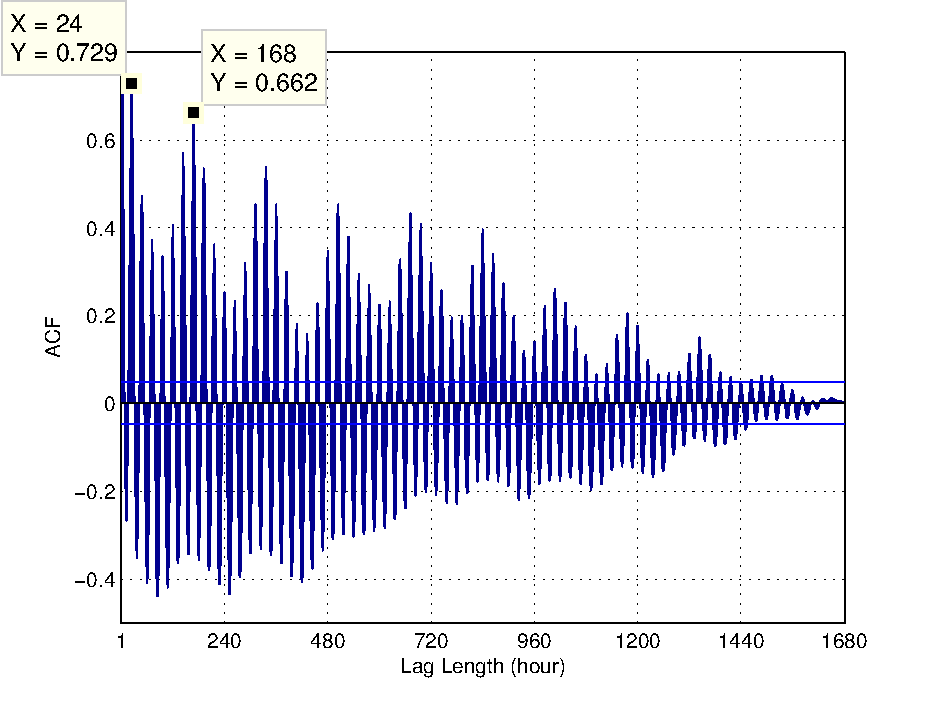
\includegraphics[width=.5\textwidth]{figs/acf_101A1_GHP-eps-converted-to.pdf}
\caption{Auto-correlation of a usual signal from the Building 1 dataset.
The signal features daily and weekly patterns (resp. $x=24$ and $x=168$).}
\label{fig:autocorr}
\end{center}
\end{figure}

An explanation for this is that the daily occupant usage patterns %office hours, 
drive these results.
Figure \ref{fig:diagram1} demonstrates this more clearly.  It shows two 1-week raw signals traces which feature the same 
diurnal pattern.  
This trend is present in almost every sensor trace, and, it hides 
the smaller fluctuations providing more specific patterns driven by local occupant activity.  Upon deeper inspection, we uncovered several
 dominant patterns, common among energy-consuming devices in buildings~\cite{wrinch:pes2012}.  Figure~\ref{fig:autocorr} depicts the 
 auto-correlation of a usual electric power signal for a device.  The two highest values in the figure correspond to a lag of 24 hours and 168 hours (one week).  
 Therefore, the signal has some periodicity and similar (though not equal) values are seen at daily and weekly time scales.
The daily pattern is due to daily office hours and the weekly pattern corresponds to weekdays and weekends.  
%Indeed, thorough inspection of the data reveals that the 
Correlation analysis on \emph{raw} signals cannot be used to determine meaningful 
inter-device relationships because periodic components act as non-stationary trends for high-frequency phenomenon, 
 making the correlation function irrelevant.  %metric is insufficient with raw signals containing the same dominant pattern.
Such trends must be removed in order to make meaningful progress towards our aforementioned goals.  

In the next section we describe SBS.  
We discuss \emph{strip and bind} in section~\ref{methodo:est}, which addresses de-trending and
relationship-discovery.  Then, we describe how we \emph{search} for changes in usage patterns, 
in section~\ref{methodo:ano}, to identify potential savings opportunities.

%One of the major challenges in this work is to discard these patterns and uncover devices intrinsic relationships.
% This difficulty is overcome by the first part of the method (Strip and Bind) presented in Section \ref{methodo:est}.
% Then, the second part of the method (Search) monitors over time the devices relationships and detect abnormal device behavior changes (Section \ref{methodo:ano}).


% \subsection{Methodology}\label{methodo}

\subsubsection{Strip and Bind} \label{methodo:est}

\begin{figure}[t!]
\begin{center}
 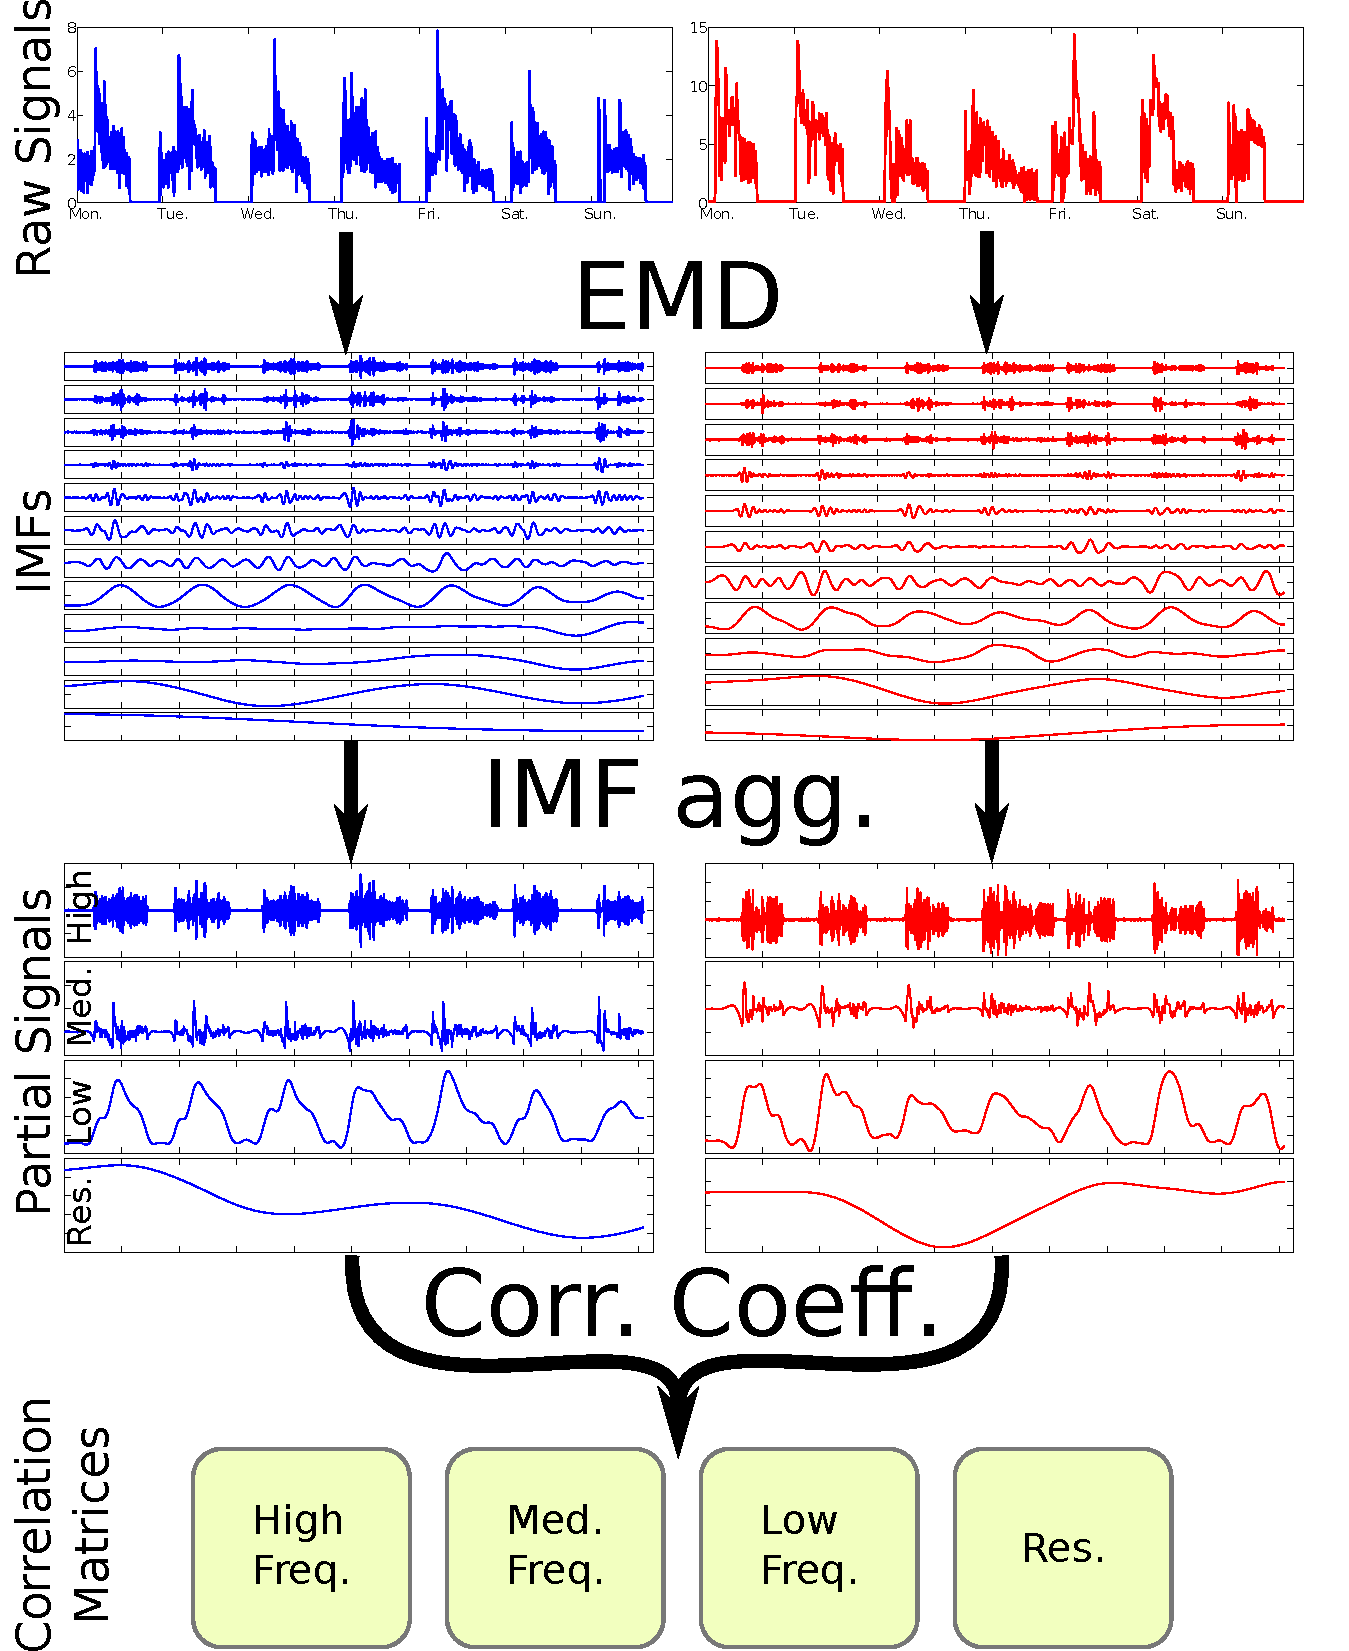
\includegraphics[width=.5\textwidth]{figs/estimator.pdf}
 \caption{\emph{Strip and Bind} using two raw signals standing for one week of data from two different HVACs. (1)~Decomposition of the signals in IMFs using EMD (top to bottom: $c_1$ to $c_n$); (2)~aggregation of the IMFs based on their time scale; (3)~comparison of the partial signals (aggregated IMFs) using correlation coefficient.}
 \label{fig:diagram1}
 \end{center}
\end{figure}

%As shown in the previous section, discovering the devices that are used in concert is particularly difficult.
Discovering devices that are used in concert is non-trivial.  
SBS decomposes each signal into an additive set of components, called Intrinsic Mode Functions (IMF), 
that reveals the signal patterns at different frequency bands.  IMFs are obtained using 
%that reveal the signal structures at different time scales.
Empirical Mode Decomposition (see Figure~\ref{fig:diagram1} and Section~\ref{emd}).
%Then, we filter out the IMFs that interfere with our goal and keep only those standing for time scales shorter than the unwanted daily pattern.
%We then remov out IMFs with time scales 
We only consider IMFs with time scales shorter than a day, since we are interested in capturing short-scale usage patterns.
Consequently, SBS aggregates the IMFs that fall into this specific time scale (see \emph{IMF agg.} in Figure \ref{fig:diagram1}).
%The resulting partial signals of different devices are compared pairwise to identify the devices intrinsic relationships (see \emph{Corr. Coeff.} in Figure\ref{fig:diagram1}). 
The resulting partial signals of different device power traces are compared, pairwise, to identify the devices that show un/correlated usage patterns (see \emph{Corr. Coeff.} in Figure~\ref{fig:diagram1}).


% These intrinsic relations are uncovered by comparing the sensors data at certain meaningful frequency bands.
% Namely, looking at high frequency allows to compare short-term variations representing the instantaneous devices change of state, however, the low frequency highlights long-term fluctuations revealing long devices usage pattern.
% 
% ..... the similarity estimators analyzes the readings from several sensors and reports scores standing for the similarity of the sensors at different frequency bands.
% First, the similarity estimator takes advantage of EMD to decompose the sensors signals into a set of components called intrinsic mode functions (IMFs).
% Second, it constructs band-limited signals by aggregating the IMFs whose mean frequencies fall in a certain frequency band.
% Thereby the pairwise comparison of band-limited signals provides the sensors correlations at different frequency bands. 
% 
% The advantages of the proposed intrinsic-correlation estimator are adaptive approach, ... 

% These two steps are described by the two following sections.



The IMFs are clustered using four time scale ranges: 
\begin{itemize}
 \item The \emph{high frequencies} are all the IMFs with a time scale lower than 20 minutes. These IMFs capture the noise.
 \item The \emph{medium frequencies} are all the IMFs with a time scale between 20 minutes and 6 hours. These IMFs convey the detailed devices usage.
 \item The \emph{low frequencies} are all the IMFs with a time scale between 6 hours and 6 days. These IMFs represent daily device patterns.
 \item The \emph{residual data} is all data with a time scale higher than 6 days. This is mainly residual data obtained after applying EMD.  Also, it highlights the main device trend.
\end{itemize}

These time scale ranges are chosen based on our experiments and goal.
The 20-minute boundary relies on the sampling period of our dataset (5 minutes) and permits us to capture IMFs with really short periods.
The 6-hour boundary allows us to analyze all patterns that have a period shorter than the usual office hours.
The 6-day boundary allows us to capture daily patterns and weekday patterns.

Aggregating IMFs, within each time scale range, results in 4 partial signals representing different characteristics of the device's
 energy consumption (see \emph{Partial Signals} in Figure~\ref{fig:diagram1}).
We do a pairwise device trace comparison, calculating the correlation coefficient of their partial signals.
In the example shown in Figure~\ref{fig:diagram1}, the correlation coefficient of the raw signals suggests that they are highly correlated ($0.57$). 
However, the comparison of the corresponding \emph{partial signals} provides new insights;
the two devices are poorly correlated at high and medium frequencies (respectively $-0.01$ and $-0.04$) but highly correlated at low frequencies ($0.79$) meaning that these devices are not ``intrinsically'' correlated.  They only share a similar daily pattern.

All the devices are compared pairwise at the four different time scale ranges.
Consequently, we obtain four correlation matrices that convey device similarities at different time scales.
Each line of these matrices (or column, since the matrices are symmetric) reveals the behavior of a device -- its relationships with the 
other devices at a particular time scale.
The matrices form the basis for tracking the behavior of devices and to search for misbehavior.


\subsection{Search}\label{methodo:ano}
\emph{Search} aims at identifying misbehaving devices in an unsupervised manner.
Device behavior is monitored via the correlation matrices presented in the previous section.
Using numerous observations SBS computes a specific reference that exhibits the normal inter-device usage pattern.
Then, SBS compares the computed reference with the current data and reports devices that deviate from their usual 
behavior.

\subsection{Reference Matrix}
We define four reference matrices, which capture normal device behavior at the four time scale ranges defined in 
Section~\ref{methodo:corr}.
The references are computed as follows: (1) we retrieve the correlation matrices for $n$ consecutive time bins. (2) For each pair of devices we compute the median correlation 
over the $n$ time bins and obtain a matrix of the median device correlations.

Formally, for each time scale range the computed reference matrix for $d$ devices and $n$ time bins is:
\[R_{i,j} =  \median(C^1_{i,j},...,C^n_{i,j})\]
where $i$ and $j$ ranges in $[1,d]$.

% Assuming that device-usage predominantly behaves normally and the anomalies are exceptional 
% events, the reference matrices exhibit the normal device behaviors.
% Our model assumes anomalies are rare and the majority of the data is normal.
% This is a common assumption in unsupervised anomaly detection.
Because anomalies are rare by definition, we assume the data used to construct the reference matrix
is an accurate sample of the population; it is unbiased and accurately captures the range of normal behavior.
% We assume that normal behavior is not truly anomalous.
Abnormal correlation values, that could appear during model construction, %in the analyzed time bins 
are ignored by the median operator thanks to its robustness to outlier (50\% breakdown point).  
However, if that assumption does not hold (more than 50\% of the data is anomalous), our model will flag the opposite -- labeling abnormal as normal and vice-versa.
From close inspection of our data, we believe our primary assumption is sound.
% Normal behavior occurs most frequently, therefore detected anomalies should be meaningful.



\subsection{Behavior change}
% SBS consists in identifying the devices that significantly deviate from their normal behaviors as defined in the reference matrices.
% Consequently, 
We compare each device behavior, for all time bins, to the one provided by the reference matrix.  
Consider the correlation matrix $C^t$ obtained from the data for time bin $t$ ($1 \leq t \leq n$).  
Vector $C^t_{i,*}$ is the behavior of the $i^{th}$ device for this time bin.
Its normal behavior is given by the corresponding vector in the reference matrix $R_{i,*}$.
We measure the device behavior change at the time bin $t$ with the following Minkowski weighted distance:
\[ l^t_{i} = \left(\sum_{j=1}^d  w_{ij}\left(C^t_{i,j} - R_{i,j}\right)^p\right)^{1/p} \]
where $d$ is the number of devices and $w_{ij}$ is:
\[ w_{ij} = \frac{R_{i,j}}{\sum_{k=1}^d R_{i,k}}. \]
The weight $w$ enables us to highlight the relationship changes between the device $i$ and those highly correlated to it in the reference matrix.
In other words, our definition of behavior change is mainly driven by the relationship among devices that are usually used in concert.
We also set $p=4$ in order to inhibit small differences between $C^t_{i,j}$ and $R_{i,j}$ but emphasize the important ones.

By monitoring this quantity over several time bins the abnormal device behaviors are easily identified as the outlier values.
In order to identify these outlier values we implement a robust detector based on median absolute deviation (MAD), a dispersion measure commonly used in anomaly detection \cite{huber:wiley2009,chan:springer2005}.
It is a measure that robustly estimates the variability of the data by computing the median of the absolute deviations from the median of the data.
 Let $l_{i} = [l_i^1,...,l_i^n]$ be a vector representing the behavior changes of device $i$ over $n$ time bins, then its MAD value is defined as:
\[ \mad_i = b \median(\lvert l_{i} - \median(l_{i})\rvert)\]
where the constant $b$ is usually set to $1.4826$ for consistency with the usual parameter $\sigma$ for Gaussian distributions.
Consequently, we define anomalous behavior, for device $i$ at time $t$, such that the following equation is satisfied:%of the device $i$ at the time bin $t$ that satisfies the following equation:
\[l^t_{i} > \median(l_{i}) + \tau  \mad_i\]
Note, $\tau$ is a parameter that permits to make SBS more or less sensitive.

The final output of SBS is a list of alarms in the form $(t,i)$ meaning that the device $i$ has abnormal behavior at the time bin $t$.
The priority of the alarms in this list is selected by the building administrator by tuning the parameter $\tau$.





We evaluate SBS using data collected from buildings in two different geographic locations.  
One is a new building on main campus of the University of Tokyo and the other is an older building at 
the University of California, Berkeley.

Data pre-processing is not generally required for the proposed approach.  
Nevertheless, we observe in a few exceptional cases that sensors reporting excessively high values (i.e. values higher than the device actual capacity) that  greatly alter the performance of SBS by inducing a large bias in the computation of the correlation coefficient.
Therefore, we remove values that are higher than the maximum capacity of the devices, from the raw data.




The Todai dataset we use contains 10 weeks of data starting from June 27, 2011 and ending on September 5, 2011.
This period of time is particularly interesting for two reasons: 1) in this region, the summer is the most energy-demanding 
season and 2) the building manager actively works to curtail energy usage as much as possible due to the 
Tohoku earthquake and Fukushima nuclear accident.

Furthermore, this dataset is a valuable ground truth to evaluate the Strip and Bind portions of SBS.
Since the light and HVAC of the rooms are directly controlled by the room's occupants, we expect SBS to uncover verifiable devices 
relationships.  


The Cory Hall dataset we use consists of 8 weeks of energy consumption traces measured by 70 sensors starting on April $5^{th}$, 2011.
In contrast to the other dataset, a variety of devices are monitored, including, electric receptacles on certain floors, most of the HVAC components, 
 power panels and whole-building consumption.

These two building infrastructures are fundamentally different.  
This enables us to evaluate the practical efficacy of the proposed, unsupervised method in two very different environments.


\begin{figure*}[t!]
% \subfloat[Raw signals]{\includegraphics[width=.48\textwidth]{img/heatMap_raw_201106-eps-converted-to.pdf}}\\
\subfloat[High Frequencies\label{fig:heatmap:high}]{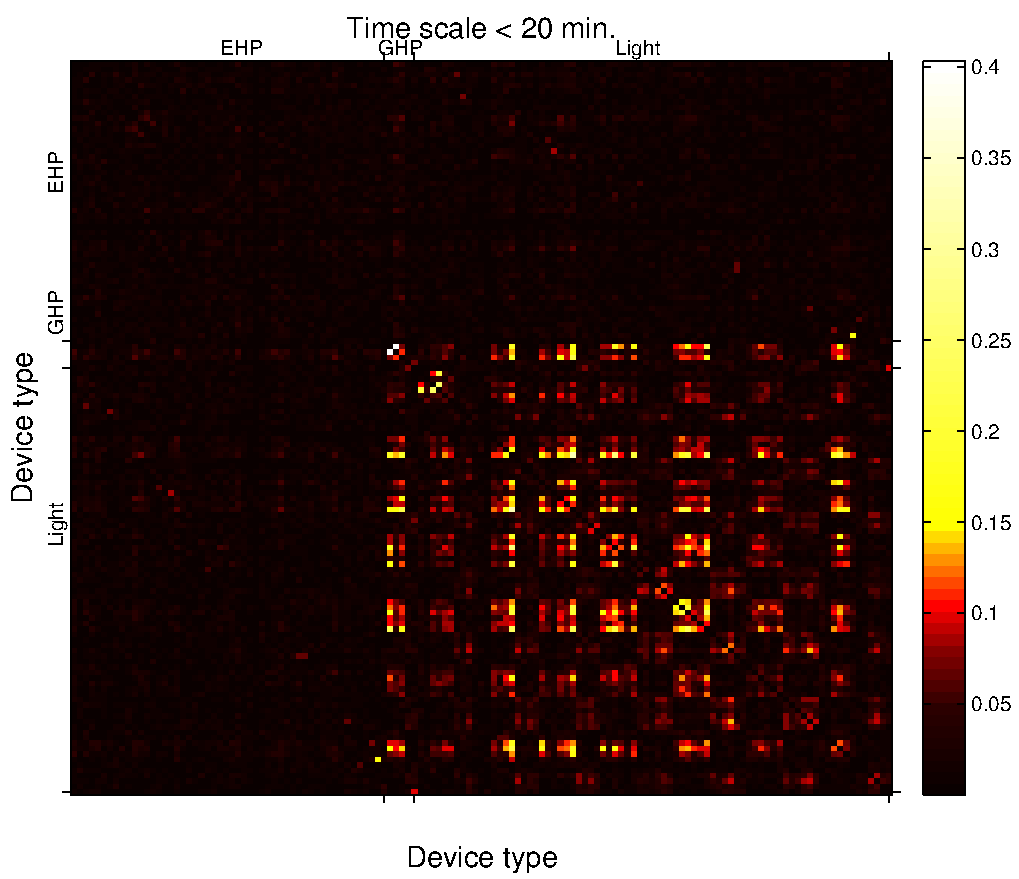
\includegraphics[width=.48\textwidth]{figs/heatMap_1_201106-eps-converted-to.pdf}}\hfill
\subfloat[Medium Frequencies\label{fig:heatmap:med}]{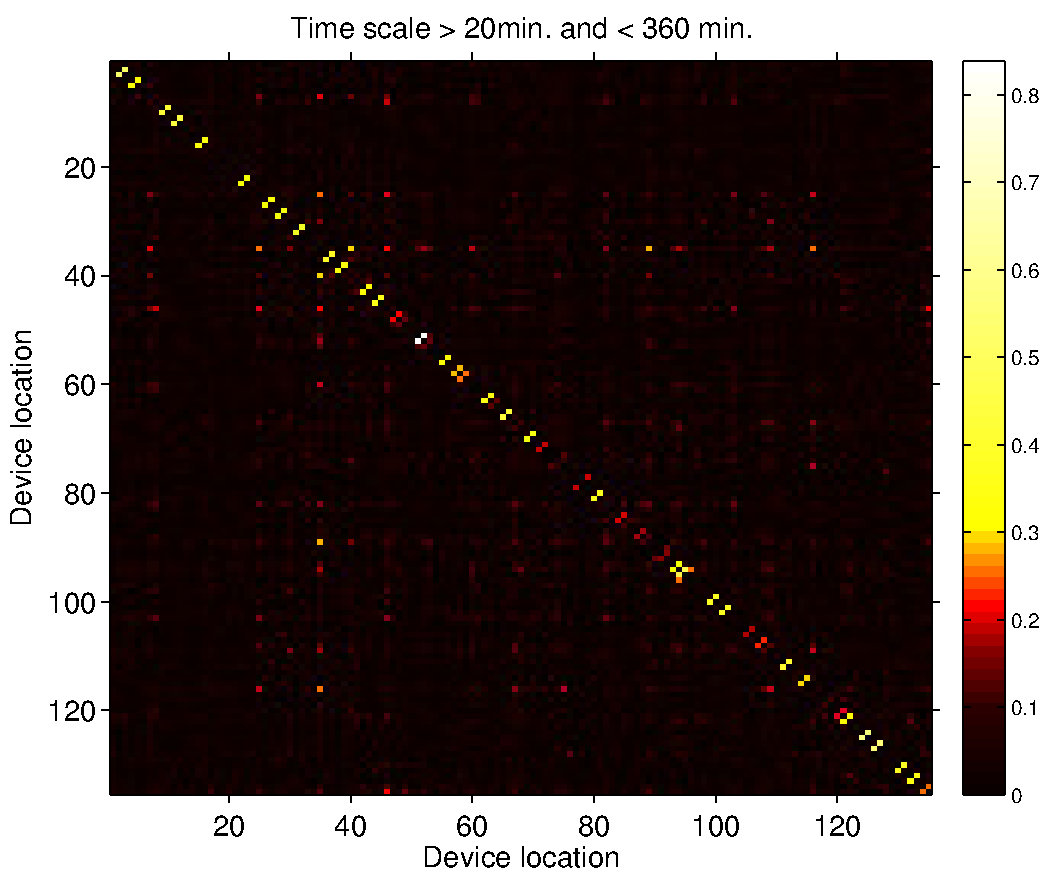
\includegraphics[width=.48\textwidth]{figs/heatMap_2_201106-eps-converted-to.pdf}}\\
\subfloat[Low Frequencies\label{fig:heatmap:low}]{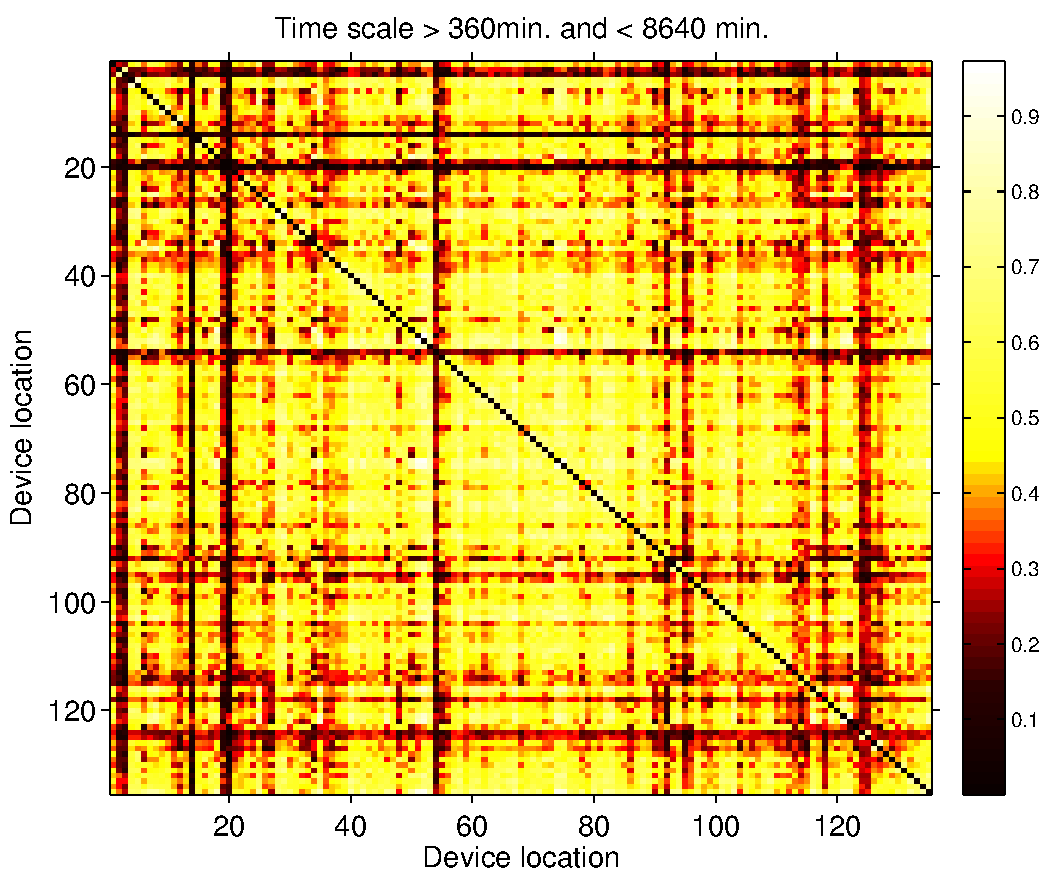
\includegraphics[width=.48\textwidth]{figs/heatMap_3_201106-eps-converted-to.pdf}}\hfill
\subfloat[Residual data\label{fig:heatmap:res}]{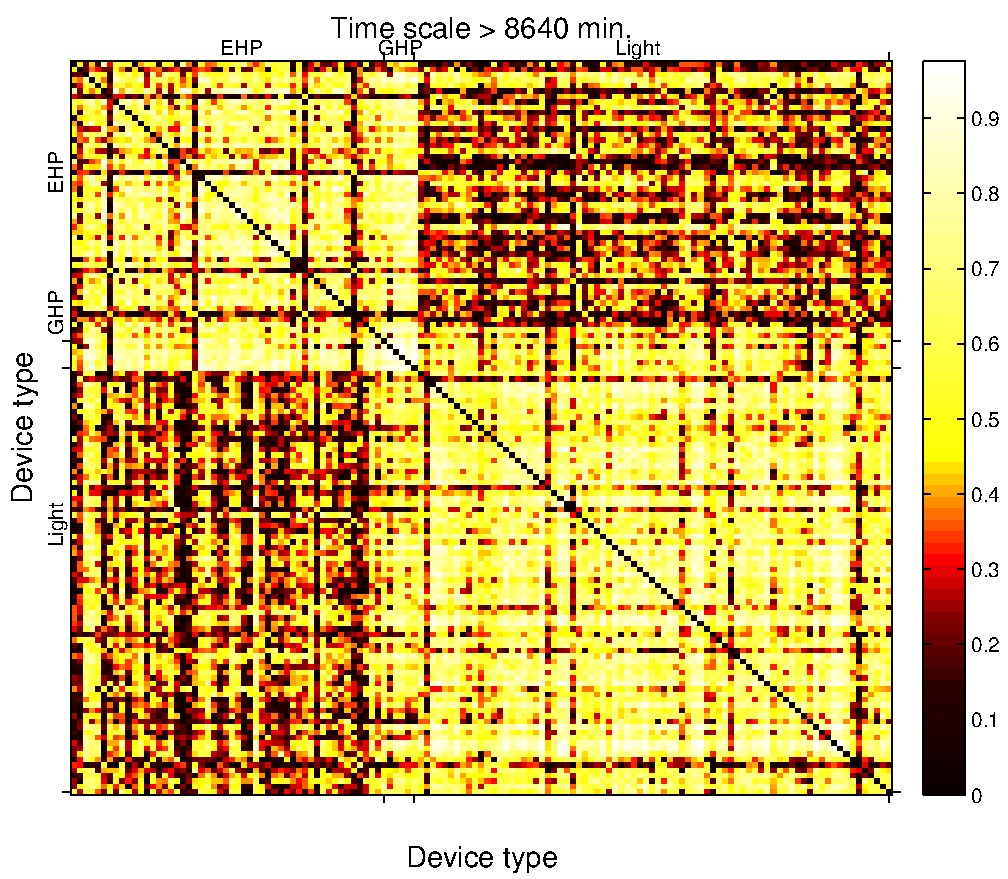
\includegraphics[width=.48\textwidth]{figs/heatMap_4_201106-eps-converted-to.pdf}}
\caption{Reference matrices for the four time scale ranges (the diagonal $x=y$ is colored in black for better reading). The medium frequencies highlight devices that are located next to each other thus intrinsically related. The low frequencies contains the common daily pattern of the data. The residual data permits to visually identify devices of the similar type.}
\label{fig:heatmap}
\end{figure*}

In this section we evaluate SBS on our building traces.  We demonstrate
 the benefits of striping the data by monitoring patterns captured at different time scales.
Then, we thoroughly investigate the alarms reported by SBS.  

\subsection{Device behavior at different time scales}
The Strip and Bind part of SBS is evaluated using the data from Eng. Bldg 2. %, since we can verify how items are being used and use it as ground truth.
This dataset is appropriate to measure SBS's performance, since lighting and HVAC systems serving the same room are usually used 
simultaneously.
Consequently, we analyze this data using SBS and verify that the higher correlations at medium frequencies correspond to devices located in the same room. % and the unwanted data is captured at the other frequencies.

The dataset is split into 10, one-week bins and each bin is processed by SBS.
Using the 10 correlation matrices at each time scale range, SBS uncovers the four reference matrices depicted in 
Figure~\ref{fig:heatmap}.

\paragraph{High frequencies}
In this work the high frequencies correspond to the signals \emph{noise}, 
therefore, we do not expect any useful information from the corresponding matrix (Figure \ref{fig:heatmap:high}).
Indeed, the corresponding reference matrix does not provide any help to determine a device's relative location.
Thus, we emphasize that high frequency data should be ignored for uncovering device relationships (in contrast to \cite{romain:iotapp12}).
Interestingly, we find that the sensors monitoring the lights generate consistent noise. % and could help one to cluster this type of sensor.
  
\paragraph{Medium frequencies}
Our main focus is on the medium frequencies as it is designed to capture the intrinsic device relationships.
Figure \ref{fig:heatmap:med} shows the correlation matrix at medium frequencies.
It is significantly different from the one obtained with the raw signals (Figure \ref{fig:heatmap:raw}): high correlation coefficients are concentrated along the matrix diagonal. 
Since devices serving the same or adjacent rooms are placed nearby in the matrix it validates our hypothesis: \emph{high correlation scores within the medium frequency band shows strong inter-device relationships}.

Considering this reference matrix as an adjacency matrix of a graph, in which the nodes are the devices, we identify the clusters of 
correlated devices using a community mining algorithm~\cite{blondel:unfolding}.
As expected we obtain mainly clusters of only two devices (light and HVAC serving the same room), but we also find clusters that are composed of more devices.
For example a cluster contains 3 HVAC systems serving the three server rooms. Although these server rooms are located on
 different floors, SBS shows a strong correlation between these devices.  Coincidentally, they are managed similarly.
Interestingly, we also observe a couple of clusters that consist of independent devices serving adjacent rooms belonging to the same lab.
The bigger cluster contains 33 devices that are 2 GHP devices and the corresponding lights.
This correlation matrix and the corresponding clusters 
highlight the ability for SBS to identify such hidden inter-device usage relationships.
 
\paragraph{Low frequencies}
Low frequencies capture daily patterns, embedded in all the device traces.  
Figure \ref{fig:heatmap:low} depicts the corresponding reference matrix which is similar to the one of raw signal traces (Figure \ref{fig:heatmap:raw}) 
and it shows no particular structure.% (daily patterns account for the coefficients high values).  
% Since this matrix contains mainly high values, most of the partial signals at low frequencies features similar characteristics (i.e. daily patterns).
These partial signals are discarded as they do not help us in identifying inter-device usage patterns.
 
\paragraph{Residual data}
The residual data shows the weekly trend, which gives us no information about device relationships.
But, surprisingly, by reordering the correlation matrix based on the type of the devices (Figure \ref{fig:heatmap:res}) 
we can visually identify two major clusters.
The first cluster consists of HVAC devices (see EHP and GHP in Figure \ref{fig:heatmap:res}) and the second one contains only lights. 
An in-depth examination of the data reveals that long-term trends are inherent to the device types. 
For example, as the consumption of both the EHP and GHP devices is driven by the building occupancy and the outside temperature, these two types of devices follow the same trend. 
However, the use of light is independent from the outside temperature thus the lighting systems follow a common trend different from the EHP and GHP one.

We conduct the same experiments by splitting the dataset in 70 bins of 1 day long and observe analogous results at high and medium frequencies but not at lower frequencies.  This is because the bins are too short to exhibit daily oscillations and the residual data captures only the daily trend.

% TODO add some info about the reference matrix for the Building 2?










\subsection{Methodological Shortcomings}
Because our analysis is done on historical data, some of the faults found by SBS could not be fully
corroborated.  In order to fully examine the effectiveness of our approach, we must run it in real time and
physically check that the problem is actually occurring.  When a problem is detected
in the historical trace, months after it has occurred, the current state of the building may no longer reflect
what is in the traces.  Some of the anomalies discussed in this section uncover interpretable patterns 
that are difficult to find in practice.  For example, simultaneous heating and cooling is a known, recurring problem
 in buildings, but it is very hard to identify  when it is occurring.  Some of the anomalies we could not interpret
might be interpretable by a building manager, however, we did not consult either building manager for this study.
Therefore, the results of this study do not examine the true/false positive rate exhaustively.

The true/false negative rate is impractical to assess.  It may be examined through synthetic stimulation of
the building via the control system.  However, getting cooperation from a building manager to hand over control of the building
for experimentation in non-trivial.  Therefore, we forgo a full true/false negative analysis in our evaluation.

Because of these challenges, the evaluation of SBS focuses on comparing the output with known fault
signatures.  We examine anomalies, in either building, where the anomaly is easily interpretable but
difficult to find by the building manager.  We forego a comparison of SBS with competing algorithms because
 related algorithms require detailed knowledge of the building, \emph{a priori}.  The advantage of SBS is that it 
requires no such information to provide immediate value.
\section{Functional Verification Experimental Results}
\label{eval}



% \subsection{Anomalies}
We evaluate the \emph{search} performance of SBS using the traces from the Eng. Bldg 2 and Cory Hall.
%% Romain
Due to the lack of historical data, such as room schedule or reports of energy waste, the evaluation is non-trivial.
Furthermore, getting ground truth data from a manual inspection of the hundreds traces of our data sets is impractical.
The lack of ground truth data prevents us from producing a systematic analysis of the anomalies missed by SBS (i.e. false negatives rate).
Nevertheless, we exhibit the relevance of the anomalies uncovered by SBS (i.e. high true positive rate and low false positive rate) by manually checking the output of SBS.
%% Romain

\paragraph{Anomaly classification}
To validate SBS results we manually inspect the anomalies detected by the algorithm.  
For each reported alarm $(t,i)$ we investigate the device trace $i$ and the devices correlated to it
to determine the reason for the alarm.
Specifically, we retrieve the major relationship change that causes the alarm (i.e. $\max(|w_j(C_{i,j}^t - R_{i,j})|)$, 
see Section \ref{methodo:ano}) and examine the metadata associated to the corresponding device.
% $j$ and the sign of the relationship change $C_{i,j}^t - R_{i,j}$.
% A positive value of relation change means the devices correlation at the time bin $t$ is abnormally high, whereas negative value means that the relationship between the two devices is broken.
This investigation allows us to classify the alarms into five groups:
\begin{itemize}
 \item \emph{High power usage}: alarms corresponding to electricity waste.
 \item \emph{Low power usage}: alarms representing the abnormally low electricity consumption of a device.
 \item \emph{Punctual abnormal usage}: alarms standing for short term (less than 2.5 hours) raise or drop of the electricity consumption.
 \item \emph{Missing data}: alarms raised due to a sensor failure.
 \item \emph{Other}: alarms whose root cause is unclear.
\end{itemize}

% However, the exhaustive enumeration of the true negatives (i.e. saving opportunities that are not detected) is impractical because of the size of the analyzed datasets (number of devices and traces length).
% Instead we exhibit the detector sensitivity by varying $\tau$, the threshold value.

\begin{figure}
\begin{center}
 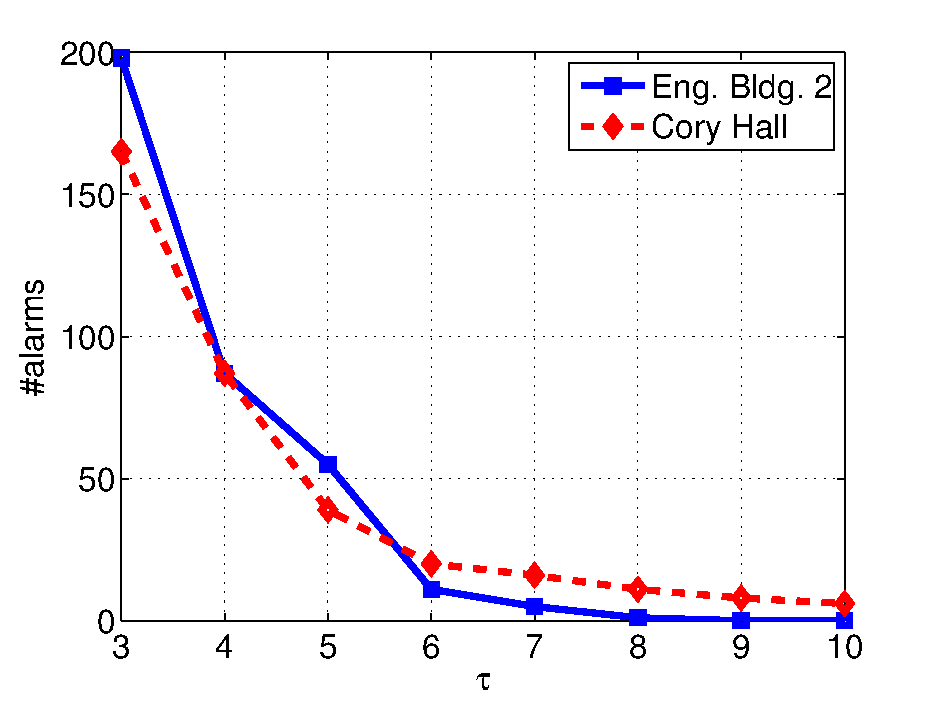
\includegraphics[width=.49\textwidth]{figs/threshold-eps-converted-to.pdf}
 \caption{Number of reported alarms for various threshold value ($\tau=[3,10]$).}
 \label{fig:thres}
 \end{center}
\end{figure}

\begin{table}
\begin{center}
\begin{tabular}{|l||c|c|c|c|c|}
\hline
&High&Low&Punc.&Missing&Other\\ \hline \hline
Eng. Bldg 2 & 9 (5) & 6 (5) & 1 (1) & 36 (1) & 3 (3) \\ \hline
Cory Hall & 25 (7) & 7 (3) & 4 (4) & 0 (0) & 3 (3) \\ \hline
\end{tabular}
\end{center}
\caption{Classification of the alarms reported by SBS for both dataset (and the number of corresponding anomalies).}
\label{tab:classif}
\end{table}

\paragraph{Experimental setup}
For each experiment, the data is split in time bins of one day, starting from 09:00 a.m. -- which is approximately 
the office's opening time.
We avoid having bins start at midnight since numerous anomalies appear at night and they are better highlighted if they are 
not spanning two time bins.
Only the data at medium frequencies are analyzed, the other frequency bands are ignored, and the reference matrix is computed from all time bins.


The threshold $\tau$ tunes the sensitivity of SBS, hence, the number of reported alarms.  
Furthermore, by plotting the number of alarms against the value of $\tau$ for both datasets (Figure \ref{fig:thres}) we observe an 
elbow in the graph around $\tau=5$.
With thresholds lower than this pivot value ($\tau<5$), the number of alarms significantly increases, causing less important anomalies 
to be reported.  
For higher values ($\tau>5$), the number of alarms is slowly decreasing, providing more conservative results that consist of the 
most important anomalies.
This pivot value provides a good trade off for either data set.

\begin{figure*}
  \subfloat[High power usage where the HVAC (EHP) is turned on at night\label{fig:res:eng1}]{\includegraphics[width=.32\textwidth]{figs/0sig20_sig31alarm1-eps-converted-to.pdf}} \hspace{.015\textwidth} %EHP turned on at night!?
  \subfloat[High power usage where the light is left on at night\label{fig:res:eng2}]{\includegraphics[width=.32\textwidth]{figs/0sig123_sig134alarm65-eps-converted-to.pdf}} \hspace{.015\textwidth}  %Light left on during night
 \subfloat[Low power usage where the HVAC (EHP) is not used during office hours\label{fig:res:eng3}]{\includegraphics[width=.32\textwidth]{figs/0sig24_sig33alarm66-eps-converted-to.pdf}}\\ %Three EHPs that are really correlated
 \subfloat[Long term high power usage partially detected\label{fig:res:eng4}]{\includegraphics[width=\textwidth]{figs/0sig3_sig15alarm7-eps-converted-to.pdf}}\\  
\caption{Example of alarms (red rectangles) reported by SBS on the Eng. Bldg 2 dataset}
\end{figure*}


Table \ref{tab:classif} classifies the alarms reported by SBS on both datasets.
 Anomalies spanning several time bins (or involving several devices) may raise several alarms.  We display these in Table \ref{tab:classif} 
 as numbers in brackets -- the number of anomalies corresponding to the reported alarms.
%Due to page limitation the following sections only present the most typical and interesting anomalies identified by SBS.

\subsection{Alarms in Todai}


SBS reported 55 alarms over the 10 weeks of the Eng. Bldg 2 dataset.
However, 36 alarms are set aside because of sensor errors; one GHP has missing data for the first 18 days.
Since this device is highly correlated to the GHP in the reference matrix, their relationship is broken for the 18 first bins and 
for each bin one alarm per device is raised.

\begin{figure*}
  \subfloat[Low power usage due to a chiller failure\label{fig:res:cory1}]{\includegraphics[width=.32\textwidth]{figs/1sig37_sig55alarm16-eps-converted-to.pdf}} \hspace{.015\textwidth}
 \subfloat[High power usage highlighted by the elevator usage\label{fig:res:cory21}]{\includegraphics[width=.32\textwidth]{figs/1sig7_sig49alarm19-eps-converted-to.pdf}}
 \hspace{.015\textwidth}
 \subfloat[Normal power and elevator usage\label{fig:res:cory22}]{\includegraphics[width=.32\textwidth]{figs/1sig7_sig49alarm-eps-converted-to.pdf}}\\ 
 \subfloat[Long term high power usage due to competing heating and cooling\label{fig:res:cory3}]{\includegraphics[width=\textwidth]{figs/1sig34_sig54alarm27-eps-converted-to.pdf}} 
\caption{Example of alarms (red rectangles) reported by SBS on the Cory Hall dataset}
\end{figure*}

In spite of the post-Fukushima measures to reduce Eng. Bldg 2's energy consumption, 
SBS reported nine alarms corresponding to high power usage (Table \ref{tab:classif}).
Figure \ref{fig:res:eng1} depicts the electricity consumption of the light and EHP in the same room where two alarms are raised.
Because the EHP was not used during daytime (but is turned on at night, when the light is turned off) the relationship between the two devices 
is ``broken'' and an alarm is raised for each device.
Figure \ref{fig:res:eng2} shows another example of energy waste.  The light is on at night and the EHP is off.
The top-priority anomaly reported by SBS is caused by the 10 days long constant use of an EHP (Figure \ref{fig:res:eng4}) and this 
waste of electricity accounts for 165 kWh.
SBS partially reports this anomaly but lower values of $\tau$ permits us to identify most of it.


We observed six alarms corresponding to abnormally low power use.  Upon further inspection we notice that it corresponds to energy saving
 initiatives from the occupants -- likely due to electricity concerns in Japan.
This behavior is displayed in Figure \ref{fig:res:eng3}.  The room is occupied at the usual office hours (indicated by light usage)  but the 
EHP is not on in order to save electricity.

\subsection{Alarms in Cory Hall}
SBS reported 39 alarms for the Cory Hall dataset (Table \ref{tab:classif}).
 Seven are classified as low power usage, however, our inspection revealed that the root causes are different than for the Eng. Bldg 2 dataset.
We observe that the low power usage usually corresponds to device failures or misconfiguration.  
For example, Figure \ref{fig:res:cory1} depicts the electricity consumption of the $2^{nd}$ floor chiller and a power riser that comprises the consumption of multiple systems, including the chiller.
As the chiller suddenly stops working, the correlation between both measurements is significantly altered and an alarm for each device is raised.

SBS also reports 25 alarms corresponding to high power usage. 
One of the identified anomalies is particularly interesting.
We indirectly observe abnormal usage of a device from the power consumption of the elevator and a power panel for equipment from 
the $1^{st}$ to the $4^{th}$ floor.
Figure~\ref{fig:res:cory21} and~\ref{fig:res:cory22} show the electricity consumption for both devices. 
SBS uncovers the correlation between the these two signals, as the amount of electricity going through the panel fluctuates along with the elevator power consumption (Figure \ref{fig:res:cory22}).
In fact, the elevator is a good indicator of the building's occupancy.
Anomalous energy-consumption is identified during a weekend as the consumption measured at the panel is independently fluctuating from the elevator usage.
These fluctuations are caused by a device that is not directly monitored.  Therefore, we could not identify the root cause more precisely. 
 Nevertheless, the alarm is worthwhile for building operators to start investigating.

The most important anomaly identified in Cory Hall is shown in Figure \ref{fig:res:cory3}.
This anomaly corresponds to the malfunctioning of the HVAC heater serving the $4^{th}$ and $5^{th}$ floors. 
The heater is constantly working for 18 consecutive days, regardless of the underlying occupant activity.
Moreover, in order to maintain appropriate temperature this also results in an increase of the $4^{th}$ floor HVAC chiller power consumption 
and several fans, such as the one depicted in Figure \ref{fig:res:cory3}.
This situation is indicative of simultaneous heating and cooling -- whereby heating and cooling systems are competing -- and it 
is a well-know problem in building management that leads to significant energy waste.
For this example, the electricity waste is estimated around 2500 kWh for the heater.
Nevertheless, as the anomaly spans over 18 days, it is hidden in the building's overall consumption, thus, it is difficult to detect 
by building administrators without SBS.

\section{Spatial Verification Methodology}

\begin{figure*}[tb]
\hspace{-2cm}
\includegraphics[width=1.2\textwidth]{figs/emd_25_26-eps-converted-to}
\vspace{-1cm}
\caption{Decomposition of the EHP and light trace using bivariate EMD. IMFs correlation coefficients highlight the intrinsic relationship of the two traces.}
\label{fig:emd}
\end{figure*}

For this investigation, we focus on a three-week span in the summer of 2011 (from July 4th to July 24th).
The dataset captures regular work days, weekends, and one holiday (July 18th).  This timeframe captures
the typical usage of the equipment, triggered by occupant activity.  For the initial
analysis, we focus on three sensors; two water pumps and a light feed.  The first pump is an 
``electric heat pump'' and is labled as EHP, the second  is a ``gas heat pump''
and labeled as GHP.  The room lighting system serves the same room as the EHP.  The GHP
serves a different room on the same floor.  The expanded portion of our analysis pivots around the EHP
and does a pairwise comparison between it and all other sensors in the building.
Computationally, this approach does not scale to a large number of sensors.  For future work, we will
examine various heuristics to narrow the search space before running pairwise comparisons.

We use EMD to detrend each of the traces and pay particularly close attention to the high-frequency IMFs.  Our 
hypothesis is that correlating at the higher frequencies will yield more meaningful comparisons.
In buildings, metadata is poorly and unsystematically managed within a single system domain.  Moreover, 
with the ever growing number of additional sub-meters, it is important to quickly integrate
sensor data from multiple systems to understand the full state of the building.  It is also important to 
understand how sensors are used in concert.  Anomalies in usage may indicate underlying problems with 
the equipment or inefficient/incorrect usage.  

Figure \ref{fig:raw} shows the raw traces for the three devices discussed in 
the previous section (EHP, GHP, light). All three exhibit a diurnal usage pattern.  On weekends, each
draw less power.   For our initial analysis, we calculated the pairwise 
correlation coefficient for all sensors in the set.  The correlation coefficient for 
 the EHP and light is $0.7715$ and the correlation coefficient for the EHP and GHP is $0.6370$.
Running correlation across them yields high correlation coefficients, mostly
due to their underlying daily usage pattern.


% \begin{figure}[t!]
% \centering
%  \subfigure[EHP trace]{\label{fig:raw_ehp}\includegraphics[width=.4\textwidth]{figs/25.png}}
%  \subfigure[Light trace]{\label{fig:raw_light}\includegraphics[width=.4\textwidth]{figs/26.png}}
%  \subfigure[GHP trace]{\label{fig:raw_ghp}\includegraphics[width=.4\textwidth]{figs/41.png}}
%  \caption{Traces from three different sensors captured in 2011 from July 4th to July 24th. Data is normalized and aggregated into 30 minutes time bins.}
%  \label{fig:raw}
% \end{figure}

\begin{figure}[ht!]
\centering
	\includegraphics[width=.4\textwidth]{figs/25.png}
\caption{Trace from an Electric Heat Pump (EHP) captured in 2011 from July 4th to July 24th. Data is 
normalized and aggregated into 30 minutes time bins.}
\label{fig:raw_ehp}
\end{figure}

\begin{figure}[ht!]
\centering
	\includegraphics[width=.4\textwidth]{figs/26.png}
\caption{Light traces from captured in 2011 from July 4th to July 24th. Data is 
normalized and aggregated into 30 minutes time bins.}
\label{fig:raw_light}
\end{figure}

\begin{figure}[ht!]
\centering
	\includegraphics[width=.4\textwidth]{figs/41.png}
\caption{Traces from a Gas Heat Pump (EHP) captured in 2011 from July 4th to July 24th. Data is 
normalized and aggregated into 30 minutes time bins.}
\label{fig:raw_ghp}
\end{figure}

\subsection{Distribution}
Let $ts^{i}_{j,t}$ be a time-series for sensor $j$ in room $i$ observed over some time interval $t$.  For simplicity, we ignore
$t$ in defining subsequent functions and re-introduce it where necessary.
For each trace we run EMD and obtain a set of $n$ IMFs, denoted as follows:
 % and applying EMD on such a trace will produce,
\begin{displaymath}
\Phi^i_j = EMD(ts^i_j) = \left \{ IMF_{1\sim n} \right \}
\end{displaymath}

IMFs are traces themselves, so we divide and re-aggregate them into the four bands, $B$,
further described in Section~\ref{sec:aggr}.
\begin{displaymath}
B = \left \{ H(igh), M(edium), L(ow), R(esidue) \right \}
\end{displaymath} 

Let the re-aggregation of the bands be denoted as:
\begin{displaymath}
Aggr(\Phi^i_j) = \left \{ IMF^i_{f,j} \right \}
\end{displaymath} 

where $f \in B$.  We pick the \emph{medium} frequency band ($M$) to compute the pairwise corrcoeff of the sensor traces. 
In order to understand and characterize the boundary between sensors we consider two sets of corrcoeffs for each room; the ``intra"-room set and 
``inter"-room set, as defined:
\begin{displaymath}
R^{i}_{intra,t} = \left \{ r(IMF^{i}_{M,j,t}, IMF^{i}_{M,k,t}) \right \}, \,
s.t.\, \forall j,k \in S_i
\end{displaymath}

The intra set only contains pairs of sensors in the same room, so both $ts^{i}_{j,t}$ and $ts^{i}_{k,t}$ are traces from 
sensors in room $i$.
\begin{displaymath}
R^{i}_{inter,t} = \left \{ r(IMF^{i}_{M,j,t}, IMF^{i'}_{M,k,t}) \right \},
\end{displaymath}
\begin{displaymath}
s.t. \, \forall j \in S_i, \, \forall k \in S_i', \, i \neq i' 
\end{displaymath}

By contrast, the \emph{inter} set contains pairs across rooms, meaning $ts_{j,t}$ is a trace from a sensor in room $i$ and 
$ts_{k,t}$ is a sensor trace from some other room $i'$.  %, and $t$ is the time span of the sensor trace the IMFs are derived from.
Note the use of $t$ in the definitions.  We re-introduce $t$ here to denote that the construction of each set is performed with respect to a specific time interval.

Finally, we examine populations, $R^i_{intra}$ and $R^i_{inter}$, across multiple time intervals (in days):%which are defined as,
\begin{displaymath}
R^{i}_{intra} = \bigcup_{\forall t}^{} R^i_{intra, t}, \; s.t. \; t \in \left \{ 1,3,5,7,14,21,28\right \}
\end{displaymath}

\begin{displaymath}
R^{i}_{inter} = \bigcup_{\forall t}^{} R^i_{inter, t}, \; s.t. \; t \in \left \{  1,3,5,7,14,21,28\right \}
\end{displaymath}

We generate a CDF for each of the two populations with respect to each room.  
This allows us to closely examine the statistical characteristics 
of the relationship between sensors in the same space and those in different spaces.  Each room offers a potentially different 
perspective on this relationship.


\subsection{Threshold Analysis}
In order to understand the statistical properties, we generate two corrcoeff distributions by computing the corrcoeff between pairs of traces within and across each room, as detailed in the previous section.
Figure~\ref{fig:group} shows how we divide the corrcoeff values into two sets.
The figure shows two intra and two inter sets. Specifically, we examine how a choice in cut-off threshold affects the ability
to separate the sets, when their separation is not known a priori, relative to each room.
Our hypothesis is that there exists a computable, statistical boundary between sensors in different rooms.

To test our hypothesis, we choose a threshold value relative to the distribution of corrcoeffs.  
All pairs with a corrcoeff larger than the threshold will be classified as being in the same room.  To closely analyze the threshold parameter, 
we generate a receiver operating characteristic (ROC) curve by varying the threshold value.  Then, we look for a good tradeoff point between the true-positive and false-positive rate; one that maximizes the difference between TPR and FPR.  We compare the ROCs generated 
for our ``medium'' frequency band IMFs against raw-signal, cross-correlation values, in order to ascertain the extent to which 
the SBS~\cite{SBS} methodology is advantageous for discovering a statistical separation, analogous to a physical one.
We also examine whether there is a uniform boundary between clusters across all the rooms. 


\begin{figure*}[ht!]
\centering
	 \includegraphics[width=0.95\textwidth]{figs/ROCgraphs}
\caption{The ROC curves depict the sensitivity of the raw signal and mid-frequency IMFs to the threshold value. We choose the 0.2 FPR point as the boundary threshold for each room. }
\label{fig:roc}
\end{figure*}



\section{Spatial Verification Results}

Our initial results on the Todai dataset were not surprising.  The diurnal pattern dominates the comparison between the sensors.
Weather is the main driver for this behavior and it affects the readings in almost all of the
sensors in our dataset.  Cross-correlation on raw sensor data is insufficient for filtering intrinsically related
behavior.  Upon closer examination of the data we assess the following:

\begin{itemize}
\item The main underlying diurnal trend occurs in almost all the traces.
\item Occupancy and room activities occur at random times during the day and change 
		at a higher frequency than weather patterns.
\item Sensors that serve the same location observe the same activities.  Therefore, their underlying
		measurements should be correlated.
\end{itemize}

In order to uncover these relationships we must remove low-frequency trends in the traces and
compare the readings at high frequencies.

\begin{table}
\begin{center}
\begin{tabular}{|l|l|l|l|l|l|}
\hline
× & Raw trace & 1st IMF & 2nd IMF & 3rd IMF & Residual\\ \hline
EHP, Light & 0.7715 & 0.43909 & 0.49344 & 0.63469 & 0.82132 \\ \hline
EHP, GHP & 0.6370 & 0.0060274 & 0.063546 & 0.16764 & 0.79378 \\ \hline
\end{tabular}
\caption{Correlation coefficients of the analyzed trace and their IMFs uncovered by EMD}
\label{tab:corr}
\end{center}
\end{table}


% \subsection{Simple Scenario}
We test our hypothesis in this section by using EMD to remove low-frequency trends in the data
and run correlation calculation at overlapping IMF timescales.  We discover that EMD allows us
to find and compare high-frequency instrinsic behavior that is spatially correlated across
sensors.  We begin with a small set of three sensors (EHP, GHP, light) and expand our scope
to include all the sensors in the dataset.







\subsection{Initial analysis}
Lets consider the simple example of Section \ref{problem} where we would like to know if the EHP trace is correlated with the two other traces.
Recall that the correlation coefficients of the raw feeds was $0.7715$ and $0.6370$, corresponding to the light 
and GHP, respectively.
As stated in previous section this result is correct but not so meaningful, since most of the traces
display the same diurnal pattern.
Figure \ref{fig:emd} and Figure \ref{fig:emd2} show the EMD decomposition of the three traces.
For each trace, EMD has retrieved three IMFs that highlight the higher frequencies of the traces.

Figure~\ref{fig:emd} shows the normalized raw trace (top) and EMD output IMFs and residual as well as the 
correlation coefficients calculated on the IMFs for the EHP and
light traces.  The correlation coefficients are $0.43909$, $0.49344$ and $0.63469$ corresponding to the IMF1, 
IMF2, and IMF3, respectively.  Notice the high correlation between the high-frequency IMFs.
We know that the light and EHP serve the same room, and their high-frequency IMF correlation corroborates
our prior knowledge.
Figure~\ref{fig:emd2} shows a complementary result, for the EHP and GHP comparison.
The correlation coefficients for the EHP and GHP IMFs suggest that the two may be independent.  In fact, they
\emph{are} indepdent; they serve completely different rooms in the building!

EMD allows us to remove low-frequency trends that add noise to the original analysis.
By comparing IMFs, we see both intrisically correlated and \emph{uncorrelated} behavior.  In the next
section we expand our analysis and show the effectiveness of our methodology. 
% Although promising, these results must be validated across the rest of the
% dataset to confirm their significance.  







\subsection{Validation}
To validate the effectiveness of our approach, we analyze the same three-week time span for \emph{all} 674 
sensors deployed in the building.
For each trace $S$ we compute two scores: (1) the correlation coefficient between $S$ and the EHP trace
and (2) the average value of the IMF correlation coefficients.

\begin{figure}[tbh!]
\centering
 \subfloat[Raw traces correlation coefficients]{\label{fig:histo1}\includegraphics[width=.43\textwidth]{figs/allFloors_week1_week4_corr_abs-eps-converted-to}}
 \subfloat[Average IMFs correlation coefficients]{\label{fig:histo2}\includegraphics[width=.43\textwidth]{figs/allFloors_week1_week4_emd_abs-eps-converted-to}}
 \caption{Distribution of the correlation coefficients of the raw traces and correlation coefficients average of the corresponding IMFs using 3 weeks of data from 674 sensors.}
\label{fig:histo}
\end{figure}

\begin{figure}
\centering
\includegraphics[width=.45\textwidth]{figs/floorMap.png}
\caption{Map of the floor where the analyzed EHP serves (room $C2$). The location of the sensors identified as related by the proposed approach are highlighted, showing a direct relationship between IMF correlation and spatial proximity.}
\label{fig:map}
\end{figure}

Figure \ref{fig:histo1} shows the distribution correlation coefficients.  Notice
that a large fraction of the dataset is correlated with the EHP trace.
\emph{Half} the traces have a correlation coefficient higher than $0.36$.  As expected, the underlying
trend is shared by a large number of device.
Although the highest score (i.e. $0.7715$) corresponds to the light in the same room that the EHP serves,
there are 118 pumps, serving all areas of the building, with a correlation higher than $0.6$.
Using only these results, it is not clear where the threshold should be set.  The distribution is close to 
uniform, making it difficult to 
know of how well your threshold discriminates against unrelated traces.
% Moreover, the distribution of the traces is almost uniform, thus, discriminating correlated traces is a laborious task.

Figure \ref{fig:histo2} shows the distribution of the average correlation value for the IMFs of
each trace and the EHP.  The number of traces correlated in the high frequency IMFs is significantly smaller
than the previous results. It's clear from the distribution that only a small set of devices are
\emph{intrinsically correlated} with the EHP.  In fact, \emph{only 10 traces out of 674} yielded a score higher than 
$0.25$. This allows us to easily rank traces by correlation.

Upon closer inspection of the 10 most correlated IMF traces, we find that there is a spatial relationship
between the EHP and the ten devices.  In fact, there is a direct relationship between score and distance from
the areas served by the EHP.  Figure~\ref{fig:map} shows a map of the floor that contains the rooms served by this
EHP.  The EHP directly serves room $C2$.  We introduce a correlation threshold to cluster correlated traces by score.
We highlight rooms by the threshold setting on the IMF correlation score.
When we set the threshold at $0.5$ we see that the sensors that have a correlation higher fall within room $C2$ --
the room served directly by the EHP.  As we relax the threshold, lowering it to $0.25$ and $0.1$ we see radial expansion from $C2$.  The trace with the highest score, $0.522$, is the trace corresponding to the lighting system \emph{in
the same room}.
The two highest scores for this floor (i.e. $0.316$ and $0.279$) are the light and EHP traces from next door, room $C1$.
Lower values correspond to sensors measuring activities in other rooms that have no specific relationship to the analyzed trace.  The results show a direct relationship between IMF correlation and spatial proximity and \emph{supports our initial
hypothesis}.

EMD is useful for finding underlying behavioral relationships between traces of sensor data.  However,
when we set the timescales smaller than a day, the results were not as strong.
The trace has to be long enough to capture the trend.  For this data set, the underlying
trend is daily, therefore it requires there to be a significant number of samples over many days.
%  to
% for this method to be effective.
Although this was a limitation for this dataset, it really depends on the underlying phenomenon that
the sensors are measuring.  Its underlying trend is ultimately what EMD will be able to separate
from the intrinsic modes of the signal.


Figure~\ref{fig:aggr1} shows a comparison of two temperature sensor feeds from different rooms and their respective
decomposition.  Despite strong correlation in the raw time series, the medium frequency IMF shows little correlation.
Only the low frequency diurnal pattern is correlated.  Alternatively,  Figure~\ref{fig:aggr2} shows a $CO_{2}$ trace and a humidity trace.

While the raw signals appear to be very different, and indeed have modest correlation, the medium frequency components
are strongly correlated.  We conjecture that the medium frequency band ``records'' local activity.  Occupants
and movement in the space affect the levels of various physical phenomenon, namely temperature, humidity, $CO_{2}$ levels, etc.
Over shorter time spans, noise in the system hides the effects of local activity.  Longer time-spans capture long-term trends 
related to weather or building operation schedules.  The medium frequency band
captures activities such as meetings and office occupation times.  
These examples illustrate the basis for an automated process.  By isolating a particular component of the signal
we seek to strip away common diurnal factors and also eliminate differences in the response of various sensors to environmental factors.
We combine this observation with a simple classifier to derive colocation.






\subsection{Spatial Clustering Experimental Results}
We conduct two sets of experiments. First, we quantify the sensitivity of our method for different threshold values 
and examine the effect of different time spans on the threshold. We then cluster the traces based on our threshold analysis 
and compare it with a baseline approach using multidimensional scaling and k-means.
% as well as with an approach combining multidimensional scaling and k-meas. 
% Last, we validate the usefulness of the proposed method in a case study.


\subsection{Baseline and Metrics}
% We exploit a simple approach as baseline to compare with our proposed approach: instead of computing the correlation coefficients between re-aggregated IMFs of sensor feeds, we directly use the raw sensor data to do the correlation analysis and generate the two distributions for thresholding approach evaluation similarly to what described previously.

% As a baseline, we perform correlation analysis on the raw data. We generate two distributions, as previously described, and observe the effects of the choice of threshold on the true/false positive rate.
As a baseline, after we generate the two distributions described previously, we apply multidimensional scaling (MDS) to the corrcoeff matrix, in order to transform the original high-dimensional relative space to a 3-D space with an absolute origin, and run the k-means clustering algorithm.
We choose the true-positive rate (TPR, also known as recall rate) and false-positive rate (FPR) as metrics to evaluate the performance of our method versus the naive approach, which correlates the raw traces. A true-positive (TP) is when a sensor pair in a room is classified as being co-located 
while a false-positive (FP) is when a sensor that is not in room is classified as being so.
%is that a sensor not in room A is clustered as in room A.

\begin{figure}[h!]
\centering
	\includegraphics[width=0.65\textwidth]{figs/Inter_intra_relationships}
\caption{Two populations are examined for our threshold analysis.  A solid line connects sensors in the same room while a dotted line connects
 to a pairs in different rooms.}
\label{fig:group}
\end{figure}

\begin{figure}[h!]
\centering
	\includegraphics[width=1.0\textwidth]{figs/corrcoeff_cdf_in_out}
\caption{CDF of correlation coefficients between IMFs of sensor feeds: the dotted lines point to some threshold which divides
 the distribution and produces a TPR and FPR.
}
\label{fig:cdf}
\end{figure}

\subsection{Characterizing the Boundary}
To corroborate our boundary-existence hypothesis, we first need to characterize the boundary between sensors in different rooms. 
We compute the pairwise correlation coefficients (corrcoeffs) between sensor traces in both of populations depicted in Figure~\ref{fig:group}, 
over different time spans -- ranging from one day to one month.
After generating points over different time 
spans for each room, we accumulate the corrcoeffs to obtain distributions as shown in Figure~\ref{fig:cdf}, for each of the five rooms. 

The dashed vertical lines in Figure~\ref{fig:cdf} 
represent an arbitrary threshold that partitions the distribution into two sets.  Pairs of sensors to the right of the line
are classified as being in the same room.  Pairs of sensors to the left are classified as being in different rooms.
The CDFs on the left column show the distribution of corrcoeffs for pairs known to be in the same room and the CDFs on the right
show the distribution of corrcoeffs in different rooms.
Note in the figure, we set the threshold to the same value to both the left and right side, in order to observe the effect of the true/false positive
rates.
By adjusting the threshold, we get different TPRs/FPRs parameterized by the threshold. Figure~\ref{fig:roc} captures the range tradeoff in a corresponding ROC curve.


Figure~\ref{fig:roc} illustrates the TPR/FPR sensitivity to different threshold values for our method and the naive approach. A good cluster achieves a high TPR and a low FPR. 
As we vary the threshold, we see that our approach 
achieves a TPR between 52\%--93\% and a FPR between 5\%--59\%.  %The baseline, mostly remains along the diagonal, meaning it is practically random. 
We can see that the average TPR for the ROC graph on the right is higher than the 
ROC graph on the left.  Moreover, the corresponding average FPR is lower on the right than on the left.
In general, as the TPR rises, the FPR also goes up -- \emph{a tradeoff exists between maximizing TPR and maintaining a lower FPR}.


 The ``boundary'' is represented as the corrcoeff that produces a ``good" TPR with an ``acceptable" FPR.  In Figure~\ref{fig:rocA}, 
  we choose 0.2 FPR as the boundary threshold.  This point represents the largest difference between TPR and FPR -- an acceptable tradeoff point. 
Looking at Figure~\ref{fig:cdf}, the 0.2 FPR corresponds roughly to the 80th-percentile correlation coefficient, on the ``inter''
set (the set of CDFs on the right).
  The recall rate for each room -- using a 80th-percentile corrcoeff threshold value -- ranges between 62\%-86\% and the 
  threshold value falls into a narrow interval between 0.1 to 0.12. This shows that \emph{we are able to choose a uniform value 
  for all the rooms regardless of the sensor type.}

\subsection{Convergence over Time}
\begin{figure}[h!]
\centering
	\includegraphics[width=0.48\textwidth]{figs/lengtheffect.eps}
\caption{The threshold values all converge to a similar value and we can derive the optimal value with as minimal as 14 days data.}
\label{fig:leneff}
\end{figure}

Using the threshold the roughly 80th-percentile corrcoeff corresponds to in the distribution, we examine how it affects the classification rate across traces
that span different lengths of time.  Convergence and consistency across different time spans is critical to automate the parameter selection
process.
Observe how the  threshold values differ quite significantly in Figure~\ref{fig:leneff}.  However, 
the threshold values 
gradually converge, as the length of training data increases from one day to one month.  The values derived after 14 days of data
are approximately the same as the final convergence value (around 0.07).  In other words, we can determine a threshold from two weeks of data.


\subsection{Clustering Results}
We cluster the sensor traces over the entire one-month period, and use the roughly 80th percentile corrceff (0.07) as the boundary threshold. 
A sensor is classified into the cluster with the largest corrcoeff. The clustering result is shown in Table~\ref{tab:cluster}.  A ``1" means the sensor is classified as inside the corresponding room. 
In general, after obtaining the sensor clusters, we don't know which room each cluster corresponds to without further information such as the metadata of sensors. The labels ``A-E" in Table~\ref{tab:cluster} are used to indicate the ground truth of where each sensor is physically placed since we have such information. Overall, the classification accuracy 
is 93.3\%.  We do not cluster on the corrcoeffs obtained among raw signals because the 80\%-percentile corrcoeff values do not converge across rooms.
The reason that we are able to get such a high accuracy, which is seemingly different from the statistics in Figure~\ref{fig:cdf} and Figure~\ref{fig:roc}, is because the statistics in the two figures are generated out of the corrcoeffs accumulated over different time spans (the same intervals in Figure~\ref{fig:leneff}) while the clustering here is performed on the corrcoeffs from the entire one-month period. 
% vary a lot and it doesn't make much sense to use different threshold for each room individually.

\begin{table}[h!]\footnotesize
 \begin{center}
	\begin{tabular}{ r|c|c|c|c|c|c }
	\multicolumn{1}{r}{}
	 &  \multicolumn{1}{c}{$A$}
	 & \multicolumn{1}{c}{$B$}
	 & \multicolumn{1}{c}{$C$}
	 & \multicolumn{1}{c}{$D$}
	  & \multicolumn{1}{c}{$E$} \\
	\cline{2-6} 
	$SensorA_{1}$ & 1 & 0 & 0 & 0 & 0 & \checkmark\\
	\cline{2-6}
	$A_{2}$ & 1 & 0 & 0 & 0 & 0 & \checkmark\\
	\cline{2-6}
	$A_{3}$ & 1 & 0 & 0 & 0 & 0 & \checkmark\\
	\cline{2-6}
	$B_{1}$ & 0 & 1 & 0 & 0 & 0 & \checkmark\\
	\cline{2-6}
	$B_{2}$ & 0 & 1 & 0 & 0 & 0 & \checkmark\\
	\cline{2-6}
	$B_{3}$ & 0 & 1 & 0 & 0 & 0 & \checkmark\\
	\cline{2-6}
	$C_{1}$ & 0 & 0 & 1 & 0 & 0 & \checkmark\\
	\cline{2-6}
	$C_{2}$ & 0 & 0 & 1 & 0 & 0 & \checkmark\\
	\cline{2-6}
	$C_{3}$ & 0 & 0 & 1 & 0 & 0 & \checkmark\\
	\cline{2-6}
	$D_{1}$ & 0 & 0 & 0 & 1 & 0 & \checkmark\\
	\cline{2-6}
	$D_{2}$ & 0 & 0 & 0 & 1 & 0 & \checkmark\\
	\cline{2-6}
	$D_{3}$ & 0 & 0 & 1 & 0 & 0 & $\times$\\
	\cline{2-6}
	$E_{1}$ & 0 & 0 & 0 & 0 & 1 & \checkmark\\
	\cline{2-6}
	$E_{2}$ & 0 & 0 & 0 & 0 & 1 & \checkmark\\
	\cline{2-6}
	$E_{3}$ & 0 & 0 & 0 & 0 & 1 & \checkmark\\
	\cline{2-6}
	\end{tabular}
 \end{center}
 \caption{Clustering result using the thresholding method: a ``1" means the sensor is classified as inside the room. We get the ``\checkmark" and ``$\times$" by comparing the clustering results with ground truth.}
 \label{tab:cluster}
\end{table}

\begin{figure*}[ht!]
\centering
	\includegraphics[width=1.0\textwidth]{figs/Space_KmeanClustering}
\caption{Clustering with k-means on the corrcoeff matrix after applying multidimensional scaling (MDS): The EMD-based set achieves an accuracy of 80\% while the results with raw-trace is only 53.3\% classification accuracy.}
\label{fig:mds}
\end{figure*}

To compare with our threshold-based method, we also cluster using a baseline approach. The pairwise corrcoeff for sensors in different rooms can be interpreted as a ``distance" between them.
A larger coefficient indicates a closer ``distance", and vice versa.  However, since the distances between pairs is relative, we use
multidimensional scaling~\cite{MDS} to find a common basis in three dimensions, re-map the relative distance metric (feature vector) into 
this three-dimensional grid and use k-means to classify the traces. % assuming the value of k is known a priori, which is the number of rooms.
We set k to equal the number of rooms, since the goal of the approach is to verify spatial placement at room-level granularity.  Generally, 
we believe that k should equal the number of rooms you wish to classify the sensors into. 
The clustering results are shown in Figure~\ref{fig:mds}.  Ground truth is shown through different markers (x, o, +, star, box). Each marker stands for one room. 
The cluster each sensor assigned to is denoted with a number. The classification accuracy of the baseline approach on corrcoeffs matrix of re-aggregated IMFs is 80\%. 
For raw traces, the baseline approach achieves an accuracy of only 53.3\%.







\section{Categorical Verification Methodology}
For categorical classification we took a use a very simple approach.  For every trace, we partition the range into 10 bins
and take the average.  We sort the bins and take the top 2 and the combine it with the average.  This combination forms
our feature vector with three components.

We run our type analysis on three data sets from separate buildings.  The first is a from the University of Tokyo.  It contain 
six types of sensors measuring power, pressure, temperature, CO2, light, and occupancy.
The other is a deployment in Sutardja Dai Hall at UC Berkeley which measures four different type that include lumens, CO2, 
temperature, and humidity.
Finally, we used a data set from Soda hall at UC Berkeley which contains 23 different types.

These data sets were chosen in such a way that we could use their categorical information to verify our approach for classifying them
according to statistical markers of categorical difference.  All the data either comes from sensors embedded in a space or a sub-system taking
a physical reading or represents a set-point setting for an actuators that control the environment.
In some cases, we are easily able to separate the stream categorically, using simple statistical summaries, while other stream -- particularly,
the ones \emph{not} actually be generated by a physical phenomenon (i.e. temperature set point) -- are statistical indistinguishable
from their physical-measurement counterpart; their differences are semantic, not behavioral.  We present our analysis and results
in this section.

\section{Type Verification Results}

\begin{figure}[t!] %htbp
\centering
\includegraphics[width=0.75\columnwidth]{figs/KETI413_co2_light_raw}
\caption{}
\label{fig:co2_light_raw}
\end{figure}

\begin{figure}[t!] %htbp
\centering
\includegraphics[width=0.75\columnwidth]{figs/EMD_LF_PCA_413_co2_light}
\caption{}
\label{fig:EMD_LF_PCA}
\end{figure}

\begin{figure}[t!] %htbp
\centering
\includegraphics[width=0.75\columnwidth]{figs/KETI413_6h_light_3IMF}
\caption{}
\label{fig:light_3IMF}
\end{figure}

\begin{figure}[t!] %htbp
\centering
\includegraphics[width=0.75\columnwidth]{figs/KETI413_co2_6h_3IMFs}
\caption{}
\label{fig:co2_3IMFs}
\end{figure}


\begin{figure}[t!] %htbp
\centering
\includegraphics[width=1.0\columnwidth]{figs/ASOvsAGN}
\caption{}
\label{fig:asovsagn}
\end{figure}

\begin{figure}[t!] %htbp
\centering
\includegraphics[width=1.0\columnwidth]{figs/temperature_streams}
\caption{}
\label{fig:tstreams}
\end{figure}


\begin{figure}[t!] %htbp
\centering
\includegraphics[width=1.0\columnwidth]{figs/VR}
\caption{}
\label{fig:tstreams}
\end{figure}

\begin{figure}[t!] %htbp
\centering
\includegraphics[width=1.0\columnwidth]{figs/gmm_centers}
\caption{}
\label{fig:tstreams}
\end{figure}

\section{Related Work}

The research community has addressed the detection of abnormal energy-consumption in buildings in numerous ways \cite{katipamula:1review2005,katipamula:2review2005}.
% Detecting abnormal energy-consumption in buildings has recently received the attention of the research community and different approaches have been studied.
% 

The rule-based techniques rely on a priori knowledge, they assert the sustainability of a system by identifying a set of undesired behaviors.
Using a hierarchical set of rules, Schein et al.\ propose a method to diagnose HVAC systems \cite{schein:hvacr2006}.
In comparison, state machine models take advantage of historical training data and domain knowledge to learn the states and transitions of a system.
The transitions are based on measured stimuli identified through a domain expertise.
State machines can model the operation of HVAC systems \cite{patnaik:toist2011} and permit to predict or detect the abnormal behavior of HVAC's components \cite{bellala:buildsys2012}.
However, the deployment of these methods require expert knowledge and are mostly applied to HVAC systems.

In~\cite{seem:energybldg2007}, the authors propose a simple unsupervised approach to monitor the average and peak daily consumption of a building and uncover outlier, nevertheless, the misbehaving devices are left unidentified.

Using regression analysis and weather variables the devices energy-consumption is predicted and abnormal usage is highlighted.
The authors of~\cite{brown:buildperf2012} use kernel regression to forecast device consumption and devices that behave differently from the predictions are reported as anomalous.
Regression models are also used with performances indices to monitor the HVAC's components and identify inefficiencies \cite{zhou:wiley2009}.
The implementation of these approaches in real situations is difficult, since it requires a training dataset and non-trivial 
parameter tuning.

Similar to our approach, previous studies identify abnormal energy-consumption using frequency analysis and unsupervised anomaly detection methods.
The device's consumption is decomposed using Fourier transform and outlier values are detected using clustering 
techniques \cite{Bellala_buildsys11,wrinch:pes2012,chen:aaaiw2011}. %jakkula
However, these methods assume a constant periodicity in the data and this causes many false positives in alarm reporting.  %, thus, they report devices usages happening at unusual times although they may not correspond to a faulty operation.
We do not make any assumption about the device usage schedule.  We only observe and model device relationships.
% We take advantage of a recent frequency analysis technique that enables us uncover the inter-device relationships~\cite{romain:iotapp12}.
% The identified anomalies correspond to devices that deviate from their normal relationship to other devices.

Reducing a building's energy consumption has also received a lot of attention from the research community.
% Since HVACs are one of the major electricity consumer in the buildings, several researchers have mainly focused on reducing the consumption of HVACs.
The most promising techniques are based on occupancy model predictions as they ensure that empty rooms are not over conditioned needlessly.
Room occupancy is usually monitored through sensor networks \cite{agarwal:ipsn2011,erickson:ipsn2011} or the computer network traffic \cite{kim:buildsys2010}.
These approaches are highly effective for buildings that have rarely-occupied rooms (e.g. conference room) and studies show that such approaches
 can achieve up to 42\% annual energy saving.
% However, these occupancy model predictions track human activity through sensor networks that usually imply the extra cost and privacy concerns.
SBS is fundamentally different from these approaches.  SBS identifies the abnormal usage of any devices rather than optimizing the normal usage of specific devices.
Nevertheless, the two approaches are complementary and energy-efficient buildings should take advantage of the synergy between them.

Recently, there has been increased interest in minimizing building energy consumption.  Our approach
differs quite substantially from related work.
Agarwal et al.~\cite{occmodels_buildsys11} present a parameter-fitting 
approach for a Gaussian model to fit the parameters of an occupancy model to match the occupancy data 
with a small data set.  
The model is then used to drive HVAC settings to reduce energy consumption.  We ignore occupancy entirely 
in our approach.  It appears as a hidden factor in the correlation patterns we observe.

Kim et al.~\cite{kim:buildsys2010} use branch-level energy monitoring and IP traffic from user's PCs to determine the
causal relationships between occupancy and energy use.  Their approach is most similar to ours.  Understanding how IP 
traffic, as a proxy for occupancy, correlates with energy use can help determine where inefficiencies may lie.

%{\bf Anomaly Detection Using Projective Markov Models in a Distributed Sensor Network~\cite{buildanomaly}}

%{\bf Duty-cycling buildings aggressively: The next frontier in HVAC control}~\cite{AgarwalBDGW11}

In each of these studies and others~\cite{kaminthermo, buildanomaly}, occupancy is used as a trigger
that drives efficient resource-usage policies.  Efficiency
when unoccupied means shutting everything off and efficiency when a space is occupied means anything
can be turned on.  There is no question that this is an excellent way to identify savings opportunities, however, we
take a fundamentally different approach.  We are agnostic to the underlying cause or driver for efficient
policies to be implemented.  More generally, we look to understand \emph{how the equipment is used in
concert}.  This may help uncover unexpected underlying relationships and can be used in an anomaly detection application
to establish ``(in)efficient'', ``(ab)normal'' usage patterns.  The latter 
should identify savings opportunities in cases where the space is unoccupied as well 
as occupied, because it has to do with the underlying behavior of the machines and how they generally work
together.  Our approach could help achieve both generality and scale for such an application.
This article focuses on the first step of this application, the identification of correlated devices.
% Our approach is flexible to be helpful when the assumption does not hold by either allowing the
% user to specify what efficient usage is or through the discovery of efficient usage over various time scales.
% In either case, the flexibility of our approach is its strength from the perspective of generality and scale.







SBS is a practical method for mining device traces, uncovering hidden relationships and abnormal behavior. 
In this paper, we validate the efficacy of SBS using the sensor metadata (i.e. device types and location), however, these 
tags are not needed by SBS to uncover devices relationships.
Furthermore, SBS requires no prior knowledge about the building and deploying our tool to other buildings requires no human intervention --
neither extra sensors nor a training dataset is needed. 

%best effort
SBS is a best effort approach that takes advantage of all the existing building sensors.
For example, our experiments revealed that SBS indirectly uncovers building occupancy through device use (e.g. the elevator in the Building 2). 
The proposed method would benefit from existing sensors that monitor room occupancy as well (e.g. those deployed in~\cite{agarwal:ipsn2011,erickson:ipsn2011}).  % albeit they are no needed.
Savings opportunities are also observable with a minimum of 2 monitored devices and building energy consumption can be better understood after using SBS.

% good=bad..
SBS constructs a model for normal inter-device behavior by looking at the usage patterns over time, thus, we run the risk that
a device that constantly misbehaves is labeled as normal.  % is considered as normal by SBS.
Nevertheless, building operators are able to quickly identify such perpetual anomalies by validating the clusters of correlated devices uncovered by SBS.
The inspection of these clusters is effortless compare to the investigation of the numerous raw traces.  
Although this kind of scenario is possible it was not observed in our experiments.
%Note, that this type of anomaly is unseen in our experiments and is expected to be rare.

%EMD
%Striping sensor data with EMD is beneficial for other work.
In this paper, we analyze only the data at medium frequencies, however, we observe that data at the high frequencies and residual data (Figure \ref{fig:heatmap}) also permits us to determine the device type.  % as well.
This information is valuable to automatically retrieve and validate device labels -- a major challenge in building metadata
management.

There has been much research work on sensor stream clustering and trace analysis. Chen and Tu~\cite{DStream} investigate 
how to cluster data streams in real-time using a density-based approach with a two-tiered framework. The first tier captures 
the dynamics of a data stream with a density decaying technique and then maps it to a grid.  The second tier computes a grid 
density based on how it clusters the grid. Their approach differs from ours in that they focus on decreasing algorithm 
complexity for real-time sensor stream clustering.  We run our analysis on historical traces and use correlation analysis
in our clustering algorithm.

Kapitanova et al.~\cite{failure} describe a technique to monitor sensor operations in the home and identify sensor failures. 
The classifier is trained on historical sensor data to obtain the relationship between sensors, assuming the number and location of 
sensors is known.  When a failure or removal of a sensor occurs, the classifier's behavior deviates and the event is captured. Our method does not require any prior knowledge and instead tries to cluster feeds to discover their relative placement.

Lu and Whitehouse~\cite{blueprints} formulate a new algorithm, particularly leveraging the semantic constraints interpreted from sensor 
data to determine sensor locations. The algorithm identifies how many rooms are present using motion sensors and determines room position based on physical constraints. Finally, it maps each sensor into the associated room. Our efforts focus on using intrinsic patterns typically pre-existing in building system sensor feeds to uncover physical relationships.

Fontugne et al.~\cite{romain:iotapp12} propose a new method to decompose sensor signals with EMD.
They extract the intrinsic usage pattern from the raw traces and show that sensors close to each other have higher intrinsic correlation. However, they do not explore the observation more deeply by answering whether there is a statistically discoverable boundary between sensor clusters in different rooms, or if there is a uniform threshold in the correlation coefficients able to be generalized to different rooms.

Fontugne et al.~\cite{SBS} carry on the work and propose an unsupervised method to monitor sensor behavior in buildings. They constructed 
a reference model out of the underlying pattens, obtained with EMD,  and use it to compare future activity against it.  They report an anomaly whenever a device deviates from the reference. This work exploits EMD as a method to detrend the signals and capture the inter-device relationships.

Much work utilizes EMD on medical data~\cite{ecg}, speech analysis~\cite{huang:signalProc2006}, image processing~\cite{ip} 
and climate analysis~\cite{climate}. Our method adopts EMD to determine whether a discoverable statistical boundary exists in sensors traces
from sensors in different rooms and whether such a boundary
 can be generalized across rooms with various kinds of sensors.
\section{Summary}


% \subsection{Functional Verification}

% future work
This chapter aims to establish a set of methodology for classifying traces and verifying that relationships specified by
users are accurate and continue to stay accurate over time.  We present empirical techniques to identify abnormalities in 
device power traces and inter-device usage patterns.
% In addition, we are planning to apply this method to online detection using, for example, a sliding window to compute an adaptive reference matrix that evolve in time.
% However, designing such system raises new challenges that are left for future work.

% The goal of this work is to assist building administrators in identifying misbehaving devices in large building sensor
% deployments.  
We proposed an unsupervised method to systematically detect abnormal energy consumption in buildings: the Strip, Bind, and Search (SBS) method.
SBS uncovers inter-device usage patterns by striping dominant trends off the devices energy-consumption trace.
Then, it monitors device usage and reports devices that deviate from the norm.  
Our main contribution is to develop an unsupervised technique to uncover the true inter-device relationships that are hidden by noise and 
dominant trends inherent to the sensor data.  
SBS is used on two sets of traces captured from two buildings with fundamentally different infrastructures.
The abnormal consumption identified in these two buildings are mainly energy waste.
The most important one is an instance of a competing heater and cooler that caused the heater to waste around 2500~kWh.


% \subsection{Spatial Verification}

EMD allows us to effectively identify fundamental relationships between sensor traces.
We believe that identifying meaningful usage-correlation patterns can help reduce oversights
by the occupants and faults that lead to energy waste.  A direct application of this is the identification
of simultaneous heating and cooling~\cite{simheatcool}.  Simultaneous heating and cooling is when the heating
and cooling system either compete with one another or compete with the incoming air from outside.  If
their combined usage is incorrect, there is major energy waste.
This problem is notoriously difficult to identify, since the occupants do not notice
changes in temperature and building management systems do not perform cross-signal comparisons.  For 
future work, we intend to run our analysis on the set of sensors that will
allow us to identify this problem: the outside temperature sensors, the cooling
coil temperature, and the air vent position sensor.  If their behavior
is not correlated as expected, an alarm will be raised.

We can also apply it to other usage scenarios.  In our traces, we found an instance where the pump
was on but the lights were off; where, typically, they are active simultaneously.
The air conditioning was pumping cool air into a room without occupants.
With our approach this could have been identified and corrected.  In future work, we intend to
package our solution to serve these kinds of applications.


This chapter we also set out to examine the underlying relationship between sensor traces to find interesting correlations
in use.  We used data from a large deployment of sensors in a building and found that direct correlation analysis on the raw
traces was not discriminatory enough to find interesting relationships.  Upon closer inspection, we noticed that
the underlying trend was dominating the correlation calculation.  In order to extract meaningful behavior this trend has
to be removed.  We show that empirical mode decomposition is a helpful analytical tool for detrending 
non-linear, non-stationary data; inherent attributes contained in our traces.

We ran our correlation analysis across IMFs, extracted from each trace by the EMD process, and found that the pump and light
that serve the same room were highly correlated, while the the other pump was not correlated to either.
In order to corroborate the applicability
of our approach, we compared the pump trace with \emph{all} 674 sensor traces and found a strong correlation
between the relative spatial position of the sensors and their IMF correlations.  The most highly-correlated IMFs were 
serving the same
area in the building.  As we relax the admittance criteria we find that the spatial correlation expands radially from
the main location served by the reference trace.

We plan to examine the use of this method in applications that help discover changes in underlying relationships over time
in order to identify opportunities for energy savings in buildings.  We will use it to build inter-device correlation models
and use these models to establish ``(ab)normal'' usage patterns.  We hope to take it a step further and include a
supervised learning approach to distinguish between ``(in)efficient'' usage patterns as well.


% \paragraph{Bi-modal Distribution} 
From the results illustrated in Figure~\ref{fig:cdf}, we observe a bi-modality in the corrcoeff 
distribution for the two population sets.  Sensors in the same room correlate to each other more (typically a corcoeff of 0.4 or higher)
than sensors in different rooms.  % have much smaller corrcoeff values. 
This bi-modal distribution may provide insight for us to 
% lays the foundation for us to 
understand the boundary and search for an effective discriminator more broadly.

% \paragraph{Across Different Sources}
To further validate the effectiveness of the proposed method, we should consider using data from different sources.
For example, in room B in Sutardja Dai Hall, there are two different sets of temperature sensors reporting data at different rates and granularities.
We demonstrate our ability to classify sensor streams on the same platform (recall the sensor box we used to collect data). 
It would be more convincing to verify the effectiveness of our method with sensor streams generated from devices on
 different systems -- since separate systems are independent.  For instance, we can use temperature data from the second deployment 
 and use the $CO_{2}$ and humidity sensor data from the first deployment and compare the results to what we have gathered.

% \paragraph{Generalizability} 
In our results, the boundary threshold parameter converges to a narrow interval, as the data set expands 
over a longer time range.  This may suggest that our method generalizes across rooms in a building, although further validation in a 
larger, more representative data set is necessary.  This study looked at 5 different rooms with a large physical separation from one
another.  A more representative data set would consider all the rooms and pay special attention to rooms that share a common orientation
and are separated by a single wall or floor slab.
  
We conjecture that local activity modulates various types of physical 
signals -- captured by the various kinds of physical sensors embedded
throughout the building -- and that those signals are attenuated
over distance and physical boundaries (such as walls).  We believe that this is what drives our observations. 
If the conjecture is true, the effects will be less pronounced in larger rooms, such as an auditorium or a large laboratory space.


As our approach performs slightly better than traditional learning techniques, we must further evaluate its robustness
versus the baseline method; across the entire building and across multiple buildings.  In future work, we will examine the 
two approaches across larger intra-building data sets and compare results across multiple buildings.
A key factor is the variance of classification accuracy -- smaller variance demonstrates robustness.  

We present a new method for spatial placement clustering.  
We first characterize the corrcoef distribution of medium frequencies IMFs between sensors in the same/different room(s), and then we learn the tradeoff between achieving a higher TPR and maintaining a lower FPR by manipulating a discriminator parameter within these two distributions. 
For a preliminary sample of relatively well separated rooms, we find that there is a clear boundary between sensor clusters in terms of their spatial placement and the boundary can be probed statistically.  We also find 
a uniform discriminator can be learned and generalized across these rooms.  
For this initial study, our method is able to classify the sensors of 93.3\% accuracy, which is 13\% higher than a tradition k-means approach, with a TPR between 62\%-86\% and a FPR less than 20\%. 

These results are very encouraging. However, we recognize that they are far from definitive. While the rooms in the study were picked arbitrarily, they are neither comprehensive nor a systematic sampling.  While they are clearly separated by our approach, and not by analyses of the raw time series, they do differ substantially in placement and usage.  A key question going forward is, ``how well will highly similar rooms be separated?"  - say, adjacent rooms facing the same side of the building and with similar occupancy. Will these techniques hold, more powerful techniques be required, or is further discrimination intractable? In future work, we will examine how far this method takes us and explore how it may be used in combination with other techniques to improve the results more generally. Automated metadata verification is important to include in the lifecycle of building data management.

We also attempt to address the categorical classification problem.  With fairly simple approaches we can use the mean and standard deviation
of the trace to classify the category of the trace, as labeled by the user.  However, for large traces with many
overlapping categories we observed that the traces are very similar and cannot be distinguished.  In order to uncover we may need out-of-band
information.  Statistically they are indistinguishable with the techniques we present.


% \subsection{Type Verification}










\chapter{Lessons Learned and Future Work}
\chapter{Conclusion}

% \appendix
% \chapter{More Monticello Candidates}

\printbibliography

\end{document}
